%%% thesis.tex --- 

%% Author: philipp@pmpc
%% Version: $Id: thesis.tex,v 0.0 2013/04/08 12:19:13 philipp Exp$

%%\revision$Header: /home/philipp/Documents/Uni/masterarbeit/thesis/thesis.tex,v 0.0 2013/04/08 12:19:13 philipp Exp$

\documentclass[letter]{report}

\usepackage[english]{babel}
\usepackage{lmodern}
\usepackage[utf8]{inputenc}
\usepackage{hyperref}
\usepackage{amsmath}
\usepackage{amssymb}
\usepackage{amsthm}
\usepackage{graphicx}
\usepackage{tikz}
\usepackage{suffix}
\usepackage{stmaryrd}
\usepackage{ifthen}
\usepackage[left=2.5cm,right=2.5cm]{geometry}
\usepackage{cite}

\usetikzlibrary{shapes.multipart,chains}
\usetikzlibrary{positioning}
\usetikzlibrary{matrix}
\usetikzlibrary{automata}
\usetikzlibrary{external} 

\newcommand{\todo}[2][]{\textcolor{red}{TODO\ifthenelse{\equal{#1}{}}{}{[#1]}: #2}}
\newcommand{\done}[2][]{\textcolor{green!50!black}{DONE\ifthenelse{\equal{#1}{}}{}{[#1]}: #2}}
\newcommand{\remark}[2][]{\textcolor{red!70!yellow}{REMARK\ifthenelse{\equal{#1}{}}{}{[#1]}: #2}}

\newtheorem{definition}{Definition}[chapter]
\newtheorem{theorem}[definition]{Theorem}
\newtheorem{lemma}[definition]{Lemma}
\newtheorem{corollary}[definition]{Corollary}
\newtheorem{conjecture}[definition]{Conjecture}

\newcommand{\E}[1]{\mathbb{E}\left[ #1 \right]}
\newcommand{\naturals}{\mathbb{N}}

\newcommand{\p}[1]{Pr\left[#1\right]}
\newcommand{\alltasks}{{\mathbb T}}
\newcommand{\neededfor}{\rightarrow}
\WithSuffix\newcommand\neededfor*{\stackrel{*}{\rightarrow}}

\tikzstyle{task_cross}=[
    {path picture={ 
        \draw[black]
        (path picture bounding box.south east) -- 
        (path picture bounding box.north west) 
        (path picture bounding box.south west) -- 
        (path picture bounding box.north east);
      }
    }
]

\tikzstyle{task_scheduled}=[fill=white, draw=black, task_cross]

% \getwidthofnode will measure the width of the node given as its second
% parameter and store it into the first parameter.
\makeatletter
\newcommand\getwidthofnode[2]{%
    \pgfextractx{#1}{\pgfpointanchor{#2}{east}}%
    \pgfextractx{\pgf@xa}{\pgfpointanchor{#2}{west}}% \pgf@xa is a length defined by PGF for temporary storage. No need to create a new temporary length.
    \addtolength{#1}{-\pgf@xa}%
}
\makeatother

\begin{document}

% profiles and stuff
\newcommand{\profile}[1]{\left\llbracket #1 \right\rrbracket}
%\newcommand{\profileones}[1]{\mathbb{1}^#1}
\newcommand{\profilerepeat}[2]{(#1)^{#2}}
\newcommand{\profileones}[1]{\profilerepeat{1}{#1}}

% stuff to draw diagrams levelwise
\newcommand{\leveltop}{0}
\newcommand{\leveltopI}{0}
\newcommand{\leveltopII}{0}
\newcommand{\leveltopIII}{0}
\newcommand{\leveltopIIII}{0}
\newcommand{\leveltopIIIII}{0}
\newcommand{\leveltopIIIIII}{0}
\newcommand{\leveltopIIIIIII}{0}
\newcommand{\leveltopIIIIIIII}{0}
\newcommand{\leveltopIIIIIIIII}{0}
\newcommand{\leveltopIIIIIIIIII}{0}
\newcommand{\leveltopIIIIIIIIIII}{0}
\newcommand{\leveltopIIIIIIIIIIII}{0}
\newcommand{\leveltopIIIIIIIIIIIII}{0}
\newcommand{\leveltopIIIIIIIIIIIIII}{0}
\newcommand{\leveltopIIIIIIIIIIIIIII}{0}
\newcommand{\leveltopIIIIIIIIIIIIIIII}{0}
\newcommand{\leveltopIIIIIIIIIIIIIIIII}{0}
\newcommand{\leveltopIIIIIIIIIIIIIIIIII}{0}
\newcommand{\leveltopIIIIIIIIIIIIIIIIIII}{0}
\newcommand{\leveltopIIIIIIIIIIIIIIIIIIII}{0}
\newcommand{\leveltopIIIIIIIIIIIIIIIIIIIII}{0}
\newcommand{\leveltopIIIIIIIIIIIIIIIIIIIIII}{0}
\newcommand{\leveltopIIIIIIIIIIIIIIIIIIIIIII}{0}
\newcommand{\leveltopIIIIIIIIIIIIIIIIIIIIIIII}{0}
\newcommand{\leveltopIIIIIIIIIIIIIIIIIIIIIIIII}{0}
\newcommand{\leveltopIIIIIIIIIIIIIIIIIIIIIIIIII}{0}
\newcommand{\leveltopIIIIIIIIIIIIIIIIIIIIIIIIIII}{0}
\newcommand{\leveltopIIIIIIIIIIIIIIIIIIIIIIIIIIII}{0}
\newcommand{\leveltopIIIIIIIIIIIIIIIIIIIIIIIIIIIII}{0}

\chapter{Theoretical foundations}
\label{chap:theoretical-foundations}

\section{Probability theory}
\label{sec:some-probability}

As we will see later, we will often be using probability distributions (in particular continuous probability distributions).

\subsection{Exponential distribution}
\label{sec:exponential-distribution}

The well-known exponential distribution is the central distribution we are dealing with in this text. All definitions and theorems within this subsection are along the lines of \cite{schickinger2001diskrete}.

\begin{definition}
  A continuous random variable is \emph{exponentially distributed} with parameter $\lambda$ if it has density 
  \begin{equation*}
    f(x) =
    \begin{cases}
      \lambda \cdot e^{-\lambda x} & \text{ if } x \geq 0 
      \\ 0 & \text{ otherwise}
    \end{cases}
    .
  \end{equation*}
\end{definition}

Note that the above definition also determines the distribution function $F$ of an exponentially distributed random variable as follows:

\begin{equation*}
  F(x) =
  \begin{cases}
    1-e^{\lambda x} & \text{ if } x \geq 0 \\
    0 & \text{ otherwise}
  \end{cases}
\end{equation*}

\begin{theorem}
  Let $X$ be an exponentially distributed random variable. Then, the expectancy of $X$ is $\E{X} = \frac 1 \lambda$.
\end{theorem}

\begin{proof}
  We can compute the expectancy for $X$ as follows:
  \begin{eqnarray*}
    \E{X} 
    &=& \int_{-\infty}^\infty x\cdot f(x)\, dx = \\
    &=& \int_{0}^\infty x\cdot \lambda e^{-\lambda x}\, dx \\
    &=& \left[ - \frac{e^{-\lambda x}\cdot \left( \lambda x + 1 \right)}{\lambda} \right]_{0}^\infty \\
    &=& \frac{1}{\lambda}
  \end{eqnarray*}
\end{proof}

\begin{theorem}[Scalability]
  Let $X$ be an exponentially distributed random variable with parameter $\lambda$ and let $a\in \mathbb{R}^+$. Then, the random variable $aX$ is exponentially distributed with parameter $\frac{\lambda}{a}$.
\end{theorem}

\begin{proof}
  We compute the probability that the random variable $aX$ is less than $x$:
  \begin{eqnarray*}
    \p{aX \leq x} 
    &=& \p{X \leq \frac{x}{a}} = \\
    &=& 1 - e^{-\frac{\lambda}{a} \cdot x}
  \end{eqnarray*}
  This result is equivalent to the density function of an exponentially distributed random variable with parameter $\frac{\lambda}{a}$.
\end{proof}

\begin{theorem}
  Let $X_1,\dots,X_n$ be exponentially-distributed random variables with respective parameters $\lambda_1,\dots,\lambda_n$. Then, the ranvom variable $Z:=\min_{i\in\left\{ 1,\dots,n \right\}} \left\{ X_i \right\}$ is exponentially distributed with parameter $\lambda=\lambda_1+\dots+\lambda_n$.
\end{theorem}

\begin{proof}
  We prove the claim by induction. 

  Suppose, we have two exponentially distributed random variables $X_1$ resp. $X_2$ with parameters $\lambda_1$ resp. $\lambda_2$. We then can compute
  \begin{align*}
    \p{min\left\{ X_1,X_2 \right\} \geq x} & = \p{X_1 \geq x \wedge X_2 \geq x} = \\ 
    & = \p{X_1 \geq x}\cdot\p{X_2 \geq x} = \\
    & = e^{-\lambda_1 x} \cdot e^{-\lambda_2 x} = \\
    & = e^{-\lambda_1 x - \lambda_2 x} = \\
    & = e^{-\left( \lambda_1+\lambda_2 \right) \cdot x},
  \end{align*}
  from which we can conclude that $\min\left\{ X_1,X_2 \right\}$ is exponentially distributed with parameter $\lambda_1 + \lambda_2$. By induction, we obtain our claim.
\end{proof}

\begin{definition}[Memorylessness]
  A random variable $X$ is called \emph{memoryless} if
  \begin{equation*}
    \p{X>t+s \mid X>s} = \p{X > t}
  \end{equation*}
\end{definition}

\begin{theorem}
  \label{sec:exponential-memoryless}
  Let $X$ be an exponentially distributed random variable with parameter $\lambda$. Then, $X$ is memoryless.
\end{theorem}

\begin{proof}
  We start by using the definition of conditional probability and rewrite until we arrive at our goal:
  \begin{eqnarray*}
    \p{X>t+s \mid X>s} &=& \frac{\p{X>t+s \wedge X>s}}{\p{X>s}} = \\
    &=& \frac{\p{X>t+s}}{\p{X>s}} = \\
    &=& \frac{e^{-\lambda \cdot(t+s)}}{e^{-\lambda s}} = \\
    &=& e^{-\lambda t} = \\
    &=& \p{X>t}
  \end{eqnarray*}
\end{proof}

This is a very advantageous property that can be exploited in our considerations to follow.

\emph{Remark:} It can even be shown that any memoryless continuous random variable is exponentially distributed, but theorem \ref{sec:exponential-memoryless} is sufficient for our needs.

\subsection{Uniform distribution}
\label{sec:uniform-distribution}

\begin{definition}
  A continuous random variable is \emph{uniformly distributed} over the interval $\left[ a,b \right]$ if it has density
  \begin{equation*}
    f(x) =
    \begin{cases}
      \frac{1}{b-a} & \text{ if } x\in\left[ a,b \right] \\
      0 & \text{ otherwise}
    \end{cases}.
  \end{equation*}
\end{definition}

The density of a uniform random variable is thus given by
\begin{equation*}
  F(x) = \begin{cases}
    0 & \text{ if } x<a \\
    \frac{x-a}{b-a} & \text{ if } x\in\left[ a,b \right] \\
    1 & \text{ if } x>b
  \end{cases}.
\end{equation*}


\subsection{General stuff}
\label{sec:probability-misc}

\begin{theorem}
  Let $X_1,\dots,X_n$ be independent, identically distributed, continuous random variables and let $i\in\left\{ 1,\dots,n \right\}$. Then 
  \begin{equation}
    \label{eq:probability-that-cont-random-variable-is-smallest-out-of-iid-is-one-over-n}
    \p{X_i = \min_{j\in\left\{ 1,\dots,n \right\}}\left\{ X_j \right\}} = \frac{1}{n}.
  \end{equation}
\end{theorem}

\begin{proof}
  It is clear that 
  \begin{equation*}
    \p{X_1 = \min_{j\in\left\{ 1,\dots,n \right\}}\left\{ X_j \right\}} = \p{X_2 = \min_{j\in\left\{ 1,\dots,n \right\}}\left\{ X_j \right\}} = \dots = \p{X_n = \min_{j\in\left\{ 1,\dots,n \right\}}\left\{ X_j \right\}},
  \end{equation*}
  because all random variables $X_1$ through $X_n$ behave the same. Thus we can deduce equation (\ref{eq:probability-that-cont-random-variable-is-smallest-out-of-iid-is-one-over-n}).
\end{proof}

\section{Graph theory}
\label{sec:foundations-graph-theory}

As we will see later, we will constantly deal with \emph{intrees}. In this section we develop simple notation for such trees. We assume that the reader is familiar with the concept of undirected trees and develop our notation on top of the one for undirected trees. For a more detailed introduction on what trees are, see e.g. \cite{diestel2005graph}.

\begin{definition}[Intree]
  Let $I'$ be a undirected tree. Let $v$ be a vertex within $I'$. Let $I$ be the directed version of $I'$ in such a way that all edges are directed towards vertex $v$. Then we call $I$ an intree or a rooted tree with root $v$.

  If there is an edge $(t_1, t_2)$ in $I$, we call $t_1$ a (direct) predecessor of $t_2$ and $t_2$ a (direct) successor of $t_1$. If there is a path from $t_1$ to $t_2$, we simply speak of predecessor and successor.
\end{definition}

Throughout this book, if not stated otherwise, we use the terms intree and tree interchangeably, because we are dealing only with intrees.

Those intrees can naturally be used to describe dependencies between different tasks, as long as each task is the requirement for at most one other tas. Each vertex in an intree then represents a task and if $t_1$ is a direct (direct) predecessor of $t_2$, this means that the task associated with $t_1$ must be executed before the task associated with $t_2$.

We can draw such intrees in a very straightforward manner: We draw the root at the bottom and its direct predecessors one level above. For each predecessor, we inductively repeat this procedure to obtain a ``top-to-bottom-description'' of the tree.

Figure \ref{fig:intree-example-task-names-directed-edges} shows an intree, where tasks 8 is a requirement for task 6, which itself is -- like task 7, 8 and (indirectly) task 10 -- a requirement for task 3. This figure also illustrates the fact that -- in an intree -- each task is a direct requirement for \emph{at most} one other task.

However, we are mostly interested in the \emph{structure} of the tree, which is why we most of the time omit the labellings of the vertices (i.e. we omit the task names) and rely on a \emph{unlabelled} representation as shown in figure \ref{fig:intree-example-structure-version}.

\begin{figure}[t]
  \centering
  \begin{subfigure}{.45\textwidth}
    \centering{}
    \begin{tikzpicture}[scale=.6, anchor=south]
      \node[circle, scale=0.9, draw] (tid0) at (3,1.5){0};
      \node[circle, scale=0.9, draw] (tid1) at (2.25,3){1};
      \node[circle, scale=0.9, draw] (tid2) at (1.5,4.5){3};
      \node[circle, scale=0.9, draw] (tid7) at (0.15,6){6};
      \node[circle, scale=0.9, draw] (tid9) at (0.15,7.5){9};
      \draw[<-, thick](tid7) -- (tid9);
      \node[circle, scale=0.9, draw] (tid10) at (1.5,6){7};
      \draw[<-, thick](tid2) -- (tid7);
      \draw[<-, thick](tid2) -- (tid10);
      \node[circle, scale=0.9, draw] (tid3) at (3.9,4.5){4};
      \node[circle, scale=0.9, draw] (tid5) at (2.85,6){8};
      \node[circle, scale=0.9, draw] (tid6) at (2.85,7.5){\small 10};
      \draw[<-, thick](tid5) -- (tid6);
      \draw[<-, thick](tid2) -- (tid5);
      \draw[<-, thick](tid1) -- (tid2);
      \draw[<-, thick](tid1) -- (tid3);
      \node[circle, scale=0.9, draw] (tid4) at (5.25,3){2};
      \node[circle, scale=0.9, draw] (tid8) at (5.25,4.5){5};
      \draw[<-, thick](tid4) -- (tid8);
      \draw[<-, thick](tid0) -- (tid1);
      \draw[<-, thick](tid0) -- (tid4);
    \end{tikzpicture}
    \caption{Labelled version with vertex labels and edges drawn as arrows.}
    \label{fig:intree-example-task-names-directed-edges}
  \end{subfigure}
  \quad
  \begin{subfigure}{.45\textwidth}
    \centering{}
    \begin{tikzpicture}[scale=.6, anchor=south]
      \node[circle, scale=0.9, fill] (tid0) at (3,1.5){};
      \node[circle, scale=0.9, fill] (tid1) at (2.25,3){};
      \node[circle, scale=0.9, fill] (tid2) at (1.5,4.5){};
      \node[circle, scale=0.9, fill] (tid7) at (0.15,6){};
      \node[circle, scale=0.9, fill] (tid9) at (0.15,7.5){};
      \draw[](tid7) -- (tid9);
      \node[circle, scale=0.9, fill] (tid10) at (1.5,6){};
      \draw[](tid2) -- (tid7);
      \draw[](tid2) -- (tid10);
      \node[circle, scale=0.9, fill] (tid3) at (3.9,4.5){};
      \node[circle, scale=0.9, fill] (tid5) at (2.85,6){};
      \node[circle, scale=0.9, fill] (tid6) at (2.85,7.5){};
      \draw[](tid5) -- (tid6);
      \draw[](tid2) -- (tid5);
      \draw[](tid1) -- (tid2);
      \draw[](tid1) -- (tid3);
      \node[circle, scale=0.9, fill] (tid4) at (5.25,3){};
      \node[circle, scale=0.9, fill] (tid8) at (5.25,4.5){};
      \draw[](tid4) -- (tid8);
      \draw[](tid0) -- (tid1);
      \draw[](tid0) -- (tid4);
      % level separators
      \draw[dashed] (0, 2.6) -- +(10, 0) node[below left, yshift=-.125cm]{Level 0};
      \draw[dashed] (0, 4.1) -- +(10, 0) node[below left, yshift=-.125cm]{Level 1};
      \draw[dashed] (0, 5.6) -- +(10, 0) node[below left, yshift=-.125cm]{Level 2};
      \draw[dashed] (0, 7.1) -- +(10, 0) node[below left, yshift=-.125cm]{Level 3};
      \draw[      ] (0, 8.6)    +(10, 0) node[below left, yshift=-.125cm]{Level 4};
    \end{tikzpicture}
    \caption{Unlabelled without arrows, edges are implicitly towards the root.}
    \label{fig:intree-example-structure-version}
  \end{subfigure}
  \caption{Graphical representation of an intree with 5 levels (numbered 0 to 4). All edges are implicitly directed towards the root, which is drawn at the bottom of the tree. Most of the time, the \emph{structure} of the tree is enough, so we will omit vertex names most of the time.}
  \label{fig:intrees-introductory-explanation}
\end{figure}

\begin{definition}[Level]
  Let $I$ be an intree. Let $v$ be a vertex within $I$. We define $level(v)$ be number of edges along the (unique) path from $v$ to the root.
\end{definition}

The concept of levels is illustrated in figure \ref{fig:intrees-introductory-explanation}.

\todo{Anzahl der rooted trees angeben.}

%%% Local Variables:
%%% TeX-master: "../thesis.tex"
%%% End: 

\chapter{First thoughts on implementation}
\label{chap:first-thoughts-on-implementation}

\section{Configuration DAG}
\label{sec:configuration-dag}

Initially we are dealing with an intree (i.e. each node has at most one successor) of tasks that have to be processed by a certain number of processors.

We will call the set of \emph{all} tasks $\alltasks$. If task $t_2$ can only be executed if $t_1$ already has been processed, we write $t_1 \neededfor t_2$. Moreover, we introduce a shorthand notation that allows us to ``chain'' several of these symbols: If there exist tasks $s_1,\dots,s_m$ ($m\in\mathbb N$), we write $t_1 \neededfor* t_2$ if we have $t_1 \neededfor s_1$ and $s_1 \neededfor s_2, s_2 \neededfor s_3, \dots, s_{m-1} \neededfor s_m$ and $s_m \neededfor t_2$ or if $t_1\neededfor t_2$ or if $t_1=t_2$.

\begin{definition}
  Let $\alltasks$ be a set of tasks, and $T \subseteq \alltasks$. We call $T$ an intree (of tasks) if there is one designated task $t_0\in\alltasks$ such that the following two conditions hold:
  \begin{eqnarray*}
    \forall  t \in T. & \quad t \neededfor* t_0 \\
    \forall  t \in T. & \quad t\neededfor s \Rightarrow s\in T
  \end{eqnarray*}
\end{definition}

\begin{definition}
  Let $T$ be an intree of tasks. Let $M\subseteq\alltasks$ be a set of tasks such that the following two conditions hold:
  \begin{itemize}
  \item $\forall t\in M.\, t \in T$
  \item $\forall t\in M.\, \nexists u \in T.\, u\neededfor t $
  \end{itemize}
  We then call the tuple $\left( T, M \right)$ a \emph{configuration}.
\end{definition}

\chapter{Drawing trees}
\label{chap:drawing-trees}

This is just a test chapter to see how we can draw the intrees and the snapshot DAGs.
\newsavebox{\nodebox}

\section{P2: A whole intree-DAG and its condensed counterpart}

%\renewcommand{\leveltopI}{-15cm + \leveltop}
\renewcommand{\leveltopII}{-15cm + \leveltopI}
\renewcommand{\leveltopIII}{-15cm + \leveltopII}
\renewcommand{\leveltopIIII}{-15cm + \leveltopIII}
\renewcommand{\leveltopIIIII}{-15cm + \leveltopIIII}
\renewcommand{\leveltopIIIIII}{-15cm + \leveltopIIIII}
\renewcommand{\leveltopIIIIIII}{-15cm + \leveltopIIIIII}
\renewcommand{\leveltopIIIIIIII}{-15cm + \leveltopIIIIIII}
\renewcommand{\leveltopIIIIIIIII}{-15cm + \leveltopIIIIIIII}
\renewcommand{\leveltopIIIIIIIIII}{-15cm + \leveltopIIIIIIIII}
\renewcommand{\leveltopIIIIIIIIIII}{-15cm + \leveltopIIIIIIIIII}
\begin{tikzpicture}[scale=.2, anchor=south]
  \begin{scope}[yshift=\leveltopI cm]
    \matrix (line1) [column sep=1cm] {
      \node[draw=black, rectangle split,  rectangle split parts=3] (sn0x104f980){
        \begin{tikzpicture}[scale=.2]
          \node[circle, scale=0.75, fill] (tid0) at (3.75,1.5){};
          \node[circle, scale=0.75, fill] (tid1) at (2.25,3){};
          \node[circle, scale=0.75, fill] (tid3) at (0.75,4.5){};
          \node[circle, scale=0.75, fill] (tid7) at (0.75,6){};
          \draw[](tid3) -- (tid7);
          \node[circle, scale=0.75, fill] (tid4) at (2.25,4.5){};
          \node[circle, scale=0.75, fill] (tid5) at (3.75,4.5){};
          \draw[](tid1) -- (tid3);
          \draw[](tid1) -- (tid4);
          \draw[](tid1) -- (tid5);
          \node[circle, scale=0.75, fill] (tid2) at (6,3){};
          \node[circle, scale=0.75, fill] (tid6) at (6,4.5){};
          \node[circle, scale=0.75, fill] (tid8) at (5.25,6){};
          \node[circle, scale=0.75, fill, red] (tid10) at (5.25,7.5){};
          \draw[](tid8) -- (tid10);
          \node[circle, scale=0.75, fill, red] (tid9) at (6.75,6){};
          \draw[](tid6) -- (tid8);
          \draw[](tid6) -- (tid9);
          \draw[](tid2) -- (tid6);
          \draw[](tid0) -- (tid1);
          \draw[](tid0) -- (tid2);
        \end{tikzpicture}
        \nodepart{two}
        \footnotesize{6.82812}
        \nodepart{three}
        \footnotesize{$50\:25\:25$}
      };
      & 
      \\
    };
  \end{scope}
  \begin{scope}[yshift=\leveltopII cm]
    \matrix (line2) [column sep=1cm] {
      \node[draw=black, rectangle split,  rectangle split parts=3] (sn0x1050190){
        \begin{tikzpicture}[scale=.2]
          \node[circle, scale=0.75, fill] (tid0) at (3,1.5){};
          \node[circle, scale=0.75, fill] (tid1) at (2.25,3){};
          \node[circle, scale=0.75, fill] (tid3) at (0.75,4.5){};
          \node[circle, scale=0.75, fill, red] (tid7) at (0.75,6){};
          \draw[](tid3) -- (tid7);
          \node[circle, scale=0.75, fill] (tid4) at (2.25,4.5){};
          \node[circle, scale=0.75, fill] (tid5) at (3.75,4.5){};
          \draw[](tid1) -- (tid3);
          \draw[](tid1) -- (tid4);
          \draw[](tid1) -- (tid5);
          \node[circle, scale=0.75, fill] (tid2) at (5.25,3){};
          \node[circle, scale=0.75, fill] (tid6) at (5.25,4.5){};
          \node[circle, scale=0.75, fill] (tid8) at (5.25,6){};
          \node[circle, scale=0.75, fill, red] (tid9) at (5.25,7.5){};
          \draw[](tid8) -- (tid9);
          \draw[](tid6) -- (tid8);
          \draw[](tid2) -- (tid6);
          \draw[](tid0) -- (tid1);
          \draw[](tid0) -- (tid2);
        \end{tikzpicture}
        \nodepart{two}
        \footnotesize{6.35938}
        \nodepart{three}
        \footnotesize{$50\:50$}
      };
      & 
      \node[draw=black, rectangle split,  rectangle split parts=3] (sn0x104cb60){
        \begin{tikzpicture}[scale=.2]
          \node[circle, scale=0.75, fill] (tid0) at (3.75,1.5){};
          \node[circle, scale=0.75, fill] (tid1) at (2.25,3){};
          \node[circle, scale=0.75, fill] (tid3) at (0.75,4.5){};
          \node[circle, scale=0.75, fill, red] (tid7) at (0.75,6){};
          \draw[](tid3) -- (tid7);
          \node[circle, scale=0.75, fill] (tid4) at (2.25,4.5){};
          \node[circle, scale=0.75, fill] (tid5) at (3.75,4.5){};
          \draw[](tid1) -- (tid3);
          \draw[](tid1) -- (tid4);
          \draw[](tid1) -- (tid5);
          \node[circle, scale=0.75, fill] (tid2) at (6,3){};
          \node[circle, scale=0.75, fill] (tid6) at (6,4.5){};
          \node[circle, scale=0.75, fill, red] (tid8) at (5.25,6){};
          \node[circle, scale=0.75, fill] (tid9) at (6.75,6){};
          \draw[](tid6) -- (tid8);
          \draw[](tid6) -- (tid9);
          \draw[](tid2) -- (tid6);
          \draw[](tid0) -- (tid1);
          \draw[](tid0) -- (tid2);
        \end{tikzpicture}
        \nodepart{two}
        \footnotesize{6.29688}
        \nodepart{three}
        \footnotesize{$50\:50$}
      };
      & 
      \node[draw=black, rectangle split,  rectangle split parts=3] (sn0x104dd20){
        \begin{tikzpicture}[scale=.2]
          \node[circle, scale=0.75, fill] (tid0) at (3.75,1.5){};
          \node[circle, scale=0.75, fill] (tid1) at (2.25,3){};
          \node[circle, scale=0.75, fill] (tid3) at (0.75,4.5){};
          \node[circle, scale=0.75, fill] (tid7) at (0.75,6){};
          \draw[](tid3) -- (tid7);
          \node[circle, scale=0.75, fill] (tid4) at (2.25,4.5){};
          \node[circle, scale=0.75, fill] (tid5) at (3.75,4.5){};
          \draw[](tid1) -- (tid3);
          \draw[](tid1) -- (tid4);
          \draw[](tid1) -- (tid5);
          \node[circle, scale=0.75, fill] (tid2) at (6,3){};
          \node[circle, scale=0.75, fill] (tid6) at (6,4.5){};
          \node[circle, scale=0.75, fill, red] (tid8) at (5.25,6){};
          \node[circle, scale=0.75, fill, red] (tid9) at (6.75,6){};
          \draw[](tid6) -- (tid8);
          \draw[](tid6) -- (tid9);
          \draw[](tid2) -- (tid6);
          \draw[](tid0) -- (tid1);
          \draw[](tid0) -- (tid2);
        \end{tikzpicture}
        \nodepart{two}
        \footnotesize{6.29688}
        \nodepart{three}
        \footnotesize{$1$}
      };
      & 
      \\
    };
  \end{scope}
  \begin{scope}[yshift=\leveltopIII cm]
    \matrix (line3) [column sep=1cm] {
      \node[draw=black, rectangle split,  rectangle split parts=3] (sn0x10519d0){
        \begin{tikzpicture}[scale=.2]
          \node[circle, scale=0.75, fill] (tid0) at (3,1.5){};
          \node[circle, scale=0.75, fill] (tid1) at (2.25,3){};
          \node[circle, scale=0.75, fill, red] (tid3) at (0.75,4.5){};
          \node[circle, scale=0.75, fill] (tid4) at (2.25,4.5){};
          \node[circle, scale=0.75, fill] (tid5) at (3.75,4.5){};
          \draw[](tid1) -- (tid3);
          \draw[](tid1) -- (tid4);
          \draw[](tid1) -- (tid5);
          \node[circle, scale=0.75, fill] (tid2) at (5.25,3){};
          \node[circle, scale=0.75, fill] (tid6) at (5.25,4.5){};
          \node[circle, scale=0.75, fill] (tid7) at (5.25,6){};
          \node[circle, scale=0.75, fill, red] (tid8) at (5.25,7.5){};
          \draw[](tid7) -- (tid8);
          \draw[](tid6) -- (tid7);
          \draw[](tid2) -- (tid6);
          \draw[](tid0) -- (tid1);
          \draw[](tid0) -- (tid2);
        \end{tikzpicture}
        \nodepart{two}
        \footnotesize{5.92188}
        \nodepart{three}
        \footnotesize{$50\:50$}
      };
      & 
      \node[draw=black, rectangle split,  rectangle split parts=3] (sn0x104fbd0){
        \begin{tikzpicture}[scale=.2]
          \node[circle, scale=0.75, fill] (tid0) at (3,1.5){};
          \node[circle, scale=0.75, fill] (tid1) at (2.25,3){};
          \node[circle, scale=0.75, fill] (tid3) at (0.75,4.5){};
          \node[circle, scale=0.75, fill, red] (tid7) at (0.75,6){};
          \draw[](tid3) -- (tid7);
          \node[circle, scale=0.75, fill] (tid4) at (2.25,4.5){};
          \node[circle, scale=0.75, fill] (tid5) at (3.75,4.5){};
          \draw[](tid1) -- (tid3);
          \draw[](tid1) -- (tid4);
          \draw[](tid1) -- (tid5);
          \node[circle, scale=0.75, fill] (tid2) at (5.25,3){};
          \node[circle, scale=0.75, fill] (tid6) at (5.25,4.5){};
          \node[circle, scale=0.75, fill, red] (tid8) at (5.25,6){};
          \draw[](tid6) -- (tid8);
          \draw[](tid2) -- (tid6);
          \draw[](tid0) -- (tid1);
          \draw[](tid0) -- (tid2);
        \end{tikzpicture}
        \nodepart{two}
        \footnotesize{5.79688}
        \nodepart{three}
        \footnotesize{$50\:33\:17$}
      };
      & 
      \node[draw=black, rectangle split,  rectangle split parts=3] (sn0x105a080){
        \begin{tikzpicture}[scale=.2]
          \node[circle, scale=0.75, fill] (tid0) at (3.75,1.5){};
          \node[circle, scale=0.75, fill] (tid1) at (2.25,3){};
          \node[circle, scale=0.75, fill] (tid3) at (0.75,4.5){};
          \node[circle, scale=0.75, fill] (tid4) at (2.25,4.5){};
          \node[circle, scale=0.75, fill] (tid5) at (3.75,4.5){};
          \draw[](tid1) -- (tid3);
          \draw[](tid1) -- (tid4);
          \draw[](tid1) -- (tid5);
          \node[circle, scale=0.75, fill] (tid2) at (6,3){};
          \node[circle, scale=0.75, fill] (tid6) at (6,4.5){};
          \node[circle, scale=0.75, fill, red] (tid7) at (5.25,6){};
          \node[circle, scale=0.75, fill, red] (tid8) at (6.75,6){};
          \draw[](tid6) -- (tid7);
          \draw[](tid6) -- (tid8);
          \draw[](tid2) -- (tid6);
          \draw[](tid0) -- (tid1);
          \draw[](tid0) -- (tid2);
        \end{tikzpicture}
        \nodepart{two}
        \footnotesize{5.79688}
        \nodepart{three}
        \footnotesize{$1$}
      };
      & 
      \\
    };
  \end{scope}
  \begin{scope}[yshift=\leveltopIIII cm]
    \matrix (line4) [column sep=1cm] {
      \node[draw=black, rectangle split,  rectangle split parts=3] (sn0x1052250){
        \begin{tikzpicture}[scale=.2]
          \node[circle, scale=0.75, fill] (tid0) at (2.25,1.5){};
          \node[circle, scale=0.75, fill] (tid1) at (0.75,3){};
          \node[circle, scale=0.75, fill] (tid3) at (0.75,4.5){};
          \node[circle, scale=0.75, fill] (tid6) at (0.75,6){};
          \node[circle, scale=0.75, fill, red] (tid7) at (0.75,7.5){};
          \draw[](tid6) -- (tid7);
          \draw[](tid3) -- (tid6);
          \draw[](tid1) -- (tid3);
          \node[circle, scale=0.75, fill] (tid2) at (3,3){};
          \node[circle, scale=0.75, fill, red] (tid4) at (2.25,4.5){};
          \node[circle, scale=0.75, fill] (tid5) at (3.75,4.5){};
          \draw[](tid2) -- (tid4);
          \draw[](tid2) -- (tid5);
          \draw[](tid0) -- (tid1);
          \draw[](tid0) -- (tid2);
        \end{tikzpicture}
        \nodepart{two}
        \footnotesize{5.54688}
        \nodepart{three}
        \footnotesize{$50\:50$}
      };
      & 
      \node[draw=black, rectangle split,  rectangle split parts=3] (sn0x1052960){
        \begin{tikzpicture}[scale=.2]
          \node[circle, scale=0.75, fill] (tid0) at (3,1.5){};
          \node[circle, scale=0.75, fill] (tid1) at (2.25,3){};
          \node[circle, scale=0.75, fill, red] (tid3) at (0.75,4.5){};
          \node[circle, scale=0.75, fill] (tid4) at (2.25,4.5){};
          \node[circle, scale=0.75, fill] (tid5) at (3.75,4.5){};
          \draw[](tid1) -- (tid3);
          \draw[](tid1) -- (tid4);
          \draw[](tid1) -- (tid5);
          \node[circle, scale=0.75, fill] (tid2) at (5.25,3){};
          \node[circle, scale=0.75, fill] (tid6) at (5.25,4.5){};
          \node[circle, scale=0.75, fill, red] (tid7) at (5.25,6){};
          \draw[](tid6) -- (tid7);
          \draw[](tid2) -- (tid6);
          \draw[](tid0) -- (tid1);
          \draw[](tid0) -- (tid2);
        \end{tikzpicture}
        \nodepart{two}
        \footnotesize{5.29688}
        \nodepart{three}
        \footnotesize{$50\:33\:17$}
      };
      & 
      \node[draw=black, rectangle split,  rectangle split parts=3] (sn0x10581e0){
        \begin{tikzpicture}[scale=.2]
          \node[circle, scale=0.75, fill] (tid0) at (3,1.5){};
          \node[circle, scale=0.75, fill] (tid1) at (2.25,3){};
          \node[circle, scale=0.75, fill] (tid3) at (0.75,4.5){};
          \node[circle, scale=0.75, fill, red] (tid7) at (0.75,6){};
          \draw[](tid3) -- (tid7);
          \node[circle, scale=0.75, fill, red] (tid4) at (2.25,4.5){};
          \node[circle, scale=0.75, fill] (tid5) at (3.75,4.5){};
          \draw[](tid1) -- (tid3);
          \draw[](tid1) -- (tid4);
          \draw[](tid1) -- (tid5);
          \node[circle, scale=0.75, fill] (tid2) at (5.25,3){};
          \node[circle, scale=0.75, fill] (tid6) at (5.25,4.5){};
          \draw[](tid2) -- (tid6);
          \draw[](tid0) -- (tid1);
          \draw[](tid0) -- (tid2);
        \end{tikzpicture}
        \nodepart{two}
        \footnotesize{5.29688}
        \nodepart{three}
        \footnotesize{$33\:17\:25\:25$}
      };
      & 
      \node[draw=black, rectangle split,  rectangle split parts=3] (sn0x1058550){
        \begin{tikzpicture}[scale=.2]
          \node[circle, scale=0.75, fill] (tid0) at (3,1.5){};
          \node[circle, scale=0.75, fill] (tid1) at (2.25,3){};
          \node[circle, scale=0.75, fill] (tid3) at (0.75,4.5){};
          \node[circle, scale=0.75, fill, red] (tid7) at (0.75,6){};
          \draw[](tid3) -- (tid7);
          \node[circle, scale=0.75, fill] (tid4) at (2.25,4.5){};
          \node[circle, scale=0.75, fill] (tid5) at (3.75,4.5){};
          \draw[](tid1) -- (tid3);
          \draw[](tid1) -- (tid4);
          \draw[](tid1) -- (tid5);
          \node[circle, scale=0.75, fill] (tid2) at (5.25,3){};
          \node[circle, scale=0.75, fill, red] (tid6) at (5.25,4.5){};
          \draw[](tid2) -- (tid6);
          \draw[](tid0) -- (tid1);
          \draw[](tid0) -- (tid2);
        \end{tikzpicture}
        \nodepart{two}
        \footnotesize{5.29688}
        \nodepart{three}
        \footnotesize{$50\:50$}
      };
      & 
      \\
    };
  \end{scope}
  \begin{scope}[yshift=\leveltopIIIII cm]
    \matrix (line5) [column sep=1cm] {
      \node[draw=black, rectangle split,  rectangle split parts=3] (sn0x10525f0){
        \begin{tikzpicture}[scale=.2]
          \node[circle, scale=0.75, fill] (tid0) at (1.5,1.5){};
          \node[circle, scale=0.75, fill] (tid1) at (0.75,3){};
          \node[circle, scale=0.75, fill] (tid3) at (0.75,4.5){};
          \node[circle, scale=0.75, fill] (tid5) at (0.75,6){};
          \node[circle, scale=0.75, fill, red] (tid6) at (0.75,7.5){};
          \draw[](tid5) -- (tid6);
          \draw[](tid3) -- (tid5);
          \draw[](tid1) -- (tid3);
          \node[circle, scale=0.75, fill] (tid2) at (2.25,3){};
          \node[circle, scale=0.75, fill, red] (tid4) at (2.25,4.5){};
          \draw[](tid2) -- (tid4);
          \draw[](tid0) -- (tid1);
          \draw[](tid0) -- (tid2);
        \end{tikzpicture}
        \nodepart{two}
        \footnotesize{5.25}
        \nodepart{three}
        \footnotesize{$50\:50$}
      };
      & 
      \node[draw=black, rectangle split,  rectangle split parts=3] (sn0x1053850){
        \begin{tikzpicture}[scale=.2]
          \node[circle, scale=0.75, fill] (tid0) at (2.25,1.5){};
          \node[circle, scale=0.75, fill] (tid1) at (1.5,3){};
          \node[circle, scale=0.75, fill, red] (tid3) at (0.75,4.5){};
          \node[circle, scale=0.75, fill] (tid4) at (2.25,4.5){};
          \draw[](tid1) -- (tid3);
          \draw[](tid1) -- (tid4);
          \node[circle, scale=0.75, fill] (tid2) at (3.75,3){};
          \node[circle, scale=0.75, fill] (tid5) at (3.75,4.5){};
          \node[circle, scale=0.75, fill, red] (tid6) at (3.75,6){};
          \draw[](tid5) -- (tid6);
          \draw[](tid2) -- (tid5);
          \draw[](tid0) -- (tid1);
          \draw[](tid0) -- (tid2);
        \end{tikzpicture}
        \nodepart{two}
        \footnotesize{4.84375}
        \nodepart{three}
        \footnotesize{$50\:25\:25$}
      };
      & 
      \node[draw=black, rectangle split,  rectangle split parts=3] (sn0x1056b00){
        \begin{tikzpicture}[scale=.2]
          \node[circle, scale=0.75, fill] (tid0) at (3,1.5){};
          \node[circle, scale=0.75, fill] (tid1) at (2.25,3){};
          \node[circle, scale=0.75, fill, red] (tid3) at (0.75,4.5){};
          \node[circle, scale=0.75, fill, red] (tid4) at (2.25,4.5){};
          \node[circle, scale=0.75, fill] (tid5) at (3.75,4.5){};
          \draw[](tid1) -- (tid3);
          \draw[](tid1) -- (tid4);
          \draw[](tid1) -- (tid5);
          \node[circle, scale=0.75, fill] (tid2) at (5.25,3){};
          \node[circle, scale=0.75, fill] (tid6) at (5.25,4.5){};
          \draw[](tid2) -- (tid6);
          \draw[](tid0) -- (tid1);
          \draw[](tid0) -- (tid2);
        \end{tikzpicture}
        \nodepart{two}
        \footnotesize{4.75}
        \nodepart{three}
        \footnotesize{$50\:50$}
      };
      & 
      \node[draw=black, rectangle split,  rectangle split parts=3] (sn0x1056fb0){
        \begin{tikzpicture}[scale=.2]
          \node[circle, scale=0.75, fill] (tid0) at (3,1.5){};
          \node[circle, scale=0.75, fill] (tid1) at (2.25,3){};
          \node[circle, scale=0.75, fill, red] (tid3) at (0.75,4.5){};
          \node[circle, scale=0.75, fill] (tid4) at (2.25,4.5){};
          \node[circle, scale=0.75, fill] (tid5) at (3.75,4.5){};
          \draw[](tid1) -- (tid3);
          \draw[](tid1) -- (tid4);
          \draw[](tid1) -- (tid5);
          \node[circle, scale=0.75, fill] (tid2) at (5.25,3){};
          \node[circle, scale=0.75, fill, red] (tid6) at (5.25,4.5){};
          \draw[](tid2) -- (tid6);
          \draw[](tid0) -- (tid1);
          \draw[](tid0) -- (tid2);
        \end{tikzpicture}
        \nodepart{two}
        \footnotesize{4.75}
        \nodepart{three}
        \footnotesize{$50\:50$}
      };
      & 
      \node[draw=black, rectangle split,  rectangle split parts=3] (sn0x1058f50){
        \begin{tikzpicture}[scale=.2]
          \node[circle, scale=0.75, fill] (tid0) at (2.25,1.5){};
          \node[circle, scale=0.75, fill] (tid1) at (1.5,3){};
          \node[circle, scale=0.75, fill] (tid3) at (0.75,4.5){};
          \node[circle, scale=0.75, fill, red] (tid6) at (0.75,6){};
          \draw[](tid3) -- (tid6);
          \node[circle, scale=0.75, fill, red] (tid4) at (2.25,4.5){};
          \draw[](tid1) -- (tid3);
          \draw[](tid1) -- (tid4);
          \node[circle, scale=0.75, fill] (tid2) at (3.75,3){};
          \node[circle, scale=0.75, fill] (tid5) at (3.75,4.5){};
          \draw[](tid2) -- (tid5);
          \draw[](tid0) -- (tid1);
          \draw[](tid0) -- (tid2);
        \end{tikzpicture}
        \nodepart{two}
        \footnotesize{4.84375}
        \nodepart{three}
        \footnotesize{$50\:25\:25$}
      };
      & 
      \node[draw=black, rectangle split,  rectangle split parts=3] (sn0x1058a50){
        \begin{tikzpicture}[scale=.2]
          \node[circle, scale=0.75, fill] (tid0) at (2.25,1.5){};
          \node[circle, scale=0.75, fill] (tid1) at (1.5,3){};
          \node[circle, scale=0.75, fill] (tid3) at (0.75,4.5){};
          \node[circle, scale=0.75, fill, red] (tid6) at (0.75,6){};
          \draw[](tid3) -- (tid6);
          \node[circle, scale=0.75, fill] (tid4) at (2.25,4.5){};
          \draw[](tid1) -- (tid3);
          \draw[](tid1) -- (tid4);
          \node[circle, scale=0.75, fill] (tid2) at (3.75,3){};
          \node[circle, scale=0.75, fill, red] (tid5) at (3.75,4.5){};
          \draw[](tid2) -- (tid5);
          \draw[](tid0) -- (tid1);
          \draw[](tid0) -- (tid2);
        \end{tikzpicture}
        \nodepart{two}
        \footnotesize{4.84375}
        \nodepart{three}
        \footnotesize{$50\:50$}
      };
      & 
      \node[draw=black, rectangle split,  rectangle split parts=3] (sn0x10597a0){
        \begin{tikzpicture}[scale=.2]
          \node[circle, scale=0.75, fill] (tid0) at (3,1.5){};
          \node[circle, scale=0.75, fill] (tid1) at (2.25,3){};
          \node[circle, scale=0.75, fill] (tid3) at (0.75,4.5){};
          \node[circle, scale=0.75, fill, red] (tid6) at (0.75,6){};
          \draw[](tid3) -- (tid6);
          \node[circle, scale=0.75, fill, red] (tid4) at (2.25,4.5){};
          \node[circle, scale=0.75, fill] (tid5) at (3.75,4.5){};
          \draw[](tid1) -- (tid3);
          \draw[](tid1) -- (tid4);
          \draw[](tid1) -- (tid5);
          \node[circle, scale=0.75, fill] (tid2) at (5.25,3){};
          \draw[](tid0) -- (tid1);
          \draw[](tid0) -- (tid2);
        \end{tikzpicture}
        \nodepart{two}
        \footnotesize{4.84375}
        \nodepart{three}
        \footnotesize{$50\:50$}
      };
      & 
      \\
    };
  \end{scope}
  \begin{scope}[yshift=\leveltopIIIIII cm]
    \matrix (line6) [column sep=1cm] {
      \node[draw=black, rectangle split,  rectangle split parts=3] (sn0x1053920){
        \begin{tikzpicture}[scale=.2]
          \node[circle, scale=0.75, fill] (tid0) at (1.5,1.5){};
          \node[circle, scale=0.75, fill] (tid1) at (0.75,3){};
          \node[circle, scale=0.75, fill] (tid3) at (0.75,4.5){};
          \node[circle, scale=0.75, fill] (tid4) at (0.75,6){};
          \node[circle, scale=0.75, fill, red] (tid5) at (0.75,7.5){};
          \draw[](tid4) -- (tid5);
          \draw[](tid3) -- (tid4);
          \draw[](tid1) -- (tid3);
          \node[circle, scale=0.75, fill, red] (tid2) at (2.25,3){};
          \draw[](tid0) -- (tid1);
          \draw[](tid0) -- (tid2);
        \end{tikzpicture}
        \nodepart{two}
        \footnotesize{5.0625}
        \nodepart{three}
        \footnotesize{$50\:50$}
      };
      & 
      \node[draw=black, rectangle split,  rectangle split parts=3] (sn0x1053bc0){
        \begin{tikzpicture}[scale=.2]
          \node[circle, scale=0.75, fill] (tid0) at (1.5,1.5){};
          \node[circle, scale=0.75, fill] (tid1) at (0.75,3){};
          \node[circle, scale=0.75, fill] (tid3) at (0.75,4.5){};
          \node[circle, scale=0.75, fill, red] (tid5) at (0.75,6){};
          \draw[](tid3) -- (tid5);
          \draw[](tid1) -- (tid3);
          \node[circle, scale=0.75, fill] (tid2) at (2.25,3){};
          \node[circle, scale=0.75, fill, red] (tid4) at (2.25,4.5){};
          \draw[](tid2) -- (tid4);
          \draw[](tid0) -- (tid1);
          \draw[](tid0) -- (tid2);
        \end{tikzpicture}
        \nodepart{two}
        \footnotesize{4.4375}
        \nodepart{three}
        \footnotesize{$50\:50$}
      };
      & 
      \node[draw=black, rectangle split,  rectangle split parts=3] (sn0x1056090){
        \begin{tikzpicture}[scale=.2]
          \node[circle, scale=0.75, fill] (tid0) at (2.25,1.5){};
          \node[circle, scale=0.75, fill] (tid1) at (1.5,3){};
          \node[circle, scale=0.75, fill, red] (tid3) at (0.75,4.5){};
          \node[circle, scale=0.75, fill, red] (tid4) at (2.25,4.5){};
          \draw[](tid1) -- (tid3);
          \draw[](tid1) -- (tid4);
          \node[circle, scale=0.75, fill] (tid2) at (3.75,3){};
          \node[circle, scale=0.75, fill] (tid5) at (3.75,4.5){};
          \draw[](tid2) -- (tid5);
          \draw[](tid0) -- (tid1);
          \draw[](tid0) -- (tid2);
        \end{tikzpicture}
        \nodepart{two}
        \footnotesize{4.25}
        \nodepart{three}
        \footnotesize{$1$}
      };
      & 
      \node[draw=black, rectangle split,  rectangle split parts=3] (sn0x1056160){
        \begin{tikzpicture}[scale=.2]
          \node[circle, scale=0.75, fill] (tid0) at (2.25,1.5){};
          \node[circle, scale=0.75, fill] (tid1) at (1.5,3){};
          \node[circle, scale=0.75, fill, red] (tid3) at (0.75,4.5){};
          \node[circle, scale=0.75, fill] (tid4) at (2.25,4.5){};
          \draw[](tid1) -- (tid3);
          \draw[](tid1) -- (tid4);
          \node[circle, scale=0.75, fill] (tid2) at (3.75,3){};
          \node[circle, scale=0.75, fill, red] (tid5) at (3.75,4.5){};
          \draw[](tid2) -- (tid5);
          \draw[](tid0) -- (tid1);
          \draw[](tid0) -- (tid2);
        \end{tikzpicture}
        \nodepart{two}
        \footnotesize{4.25}
        \nodepart{three}
        \footnotesize{$50\:50$}
      };
      & 
      \node[draw=black, rectangle split,  rectangle split parts=3] (sn0x1057630){
        \begin{tikzpicture}[scale=.2]
          \node[circle, scale=0.75, fill] (tid0) at (3,1.5){};
          \node[circle, scale=0.75, fill] (tid1) at (2.25,3){};
          \node[circle, scale=0.75, fill, red] (tid3) at (0.75,4.5){};
          \node[circle, scale=0.75, fill, red] (tid4) at (2.25,4.5){};
          \node[circle, scale=0.75, fill] (tid5) at (3.75,4.5){};
          \draw[](tid1) -- (tid3);
          \draw[](tid1) -- (tid4);
          \draw[](tid1) -- (tid5);
          \node[circle, scale=0.75, fill] (tid2) at (5.25,3){};
          \draw[](tid0) -- (tid1);
          \draw[](tid0) -- (tid2);
        \end{tikzpicture}
        \nodepart{two}
        \footnotesize{4.25}
        \nodepart{three}
        \footnotesize{$1$}
      };
      & 
      \node[draw=black, rectangle split,  rectangle split parts=3] (sn0x1058b20){
        \begin{tikzpicture}[scale=.2]
          \node[circle, scale=0.75, fill] (tid0) at (2.25,1.5){};
          \node[circle, scale=0.75, fill] (tid1) at (1.5,3){};
          \node[circle, scale=0.75, fill] (tid3) at (0.75,4.5){};
          \node[circle, scale=0.75, fill, red] (tid5) at (0.75,6){};
          \draw[](tid3) -- (tid5);
          \node[circle, scale=0.75, fill, red] (tid4) at (2.25,4.5){};
          \draw[](tid1) -- (tid3);
          \draw[](tid1) -- (tid4);
          \node[circle, scale=0.75, fill] (tid2) at (3.75,3){};
          \draw[](tid0) -- (tid1);
          \draw[](tid0) -- (tid2);
        \end{tikzpicture}
        \nodepart{two}
        \footnotesize{4.4375}
        \nodepart{three}
        \footnotesize{$50\:50$}
      };
      & 
      \\
    };
  \end{scope}
  \begin{scope}[yshift=\leveltopIIIIIII cm]
    \matrix (line7) [column sep=1cm] {
      \node[draw=black, rectangle split,  rectangle split parts=3] (sn0x10540d0){
        \begin{tikzpicture}[scale=.2]
          \node[circle, scale=0.75, fill] (tid0) at (0.75,1.5){};
          \node[circle, scale=0.75, fill] (tid1) at (0.75,3){};
          \node[circle, scale=0.75, fill] (tid2) at (0.75,4.5){};
          \node[circle, scale=0.75, fill] (tid3) at (0.75,6){};
          \node[circle, scale=0.75, fill, red] (tid4) at (0.75,7.5){};
          \draw[](tid3) -- (tid4);
          \draw[](tid2) -- (tid3);
          \draw[](tid1) -- (tid2);
          \draw[](tid0) -- (tid1);
        \end{tikzpicture}
        \nodepart{two}
        \footnotesize{5}
        \nodepart{three}
        \footnotesize{$1$}
      };
      & 
      \node[draw=black, rectangle split,  rectangle split parts=3] (sn0x1054480){
        \begin{tikzpicture}[scale=.2]
          \node[circle, scale=0.75, fill] (tid0) at (1.5,1.5){};
          \node[circle, scale=0.75, fill] (tid1) at (0.75,3){};
          \node[circle, scale=0.75, fill] (tid3) at (0.75,4.5){};
          \node[circle, scale=0.75, fill, red] (tid4) at (0.75,6){};
          \draw[](tid3) -- (tid4);
          \draw[](tid1) -- (tid3);
          \node[circle, scale=0.75, fill, red] (tid2) at (2.25,3){};
          \draw[](tid0) -- (tid1);
          \draw[](tid0) -- (tid2);
        \end{tikzpicture}
        \nodepart{two}
        \footnotesize{4.125}
        \nodepart{three}
        \footnotesize{$50\:50$}
      };
      & 
      \node[draw=black, rectangle split,  rectangle split parts=3] (sn0x1055dd0){
        \begin{tikzpicture}[scale=.2]
          \node[circle, scale=0.75, fill] (tid0) at (1.5,1.5){};
          \node[circle, scale=0.75, fill] (tid1) at (0.75,3){};
          \node[circle, scale=0.75, fill, red] (tid3) at (0.75,4.5){};
          \draw[](tid1) -- (tid3);
          \node[circle, scale=0.75, fill] (tid2) at (2.25,3){};
          \node[circle, scale=0.75, fill, red] (tid4) at (2.25,4.5){};
          \draw[](tid2) -- (tid4);
          \draw[](tid0) -- (tid1);
          \draw[](tid0) -- (tid2);
        \end{tikzpicture}
        \nodepart{two}
        \footnotesize{3.75}
        \nodepart{three}
        \footnotesize{$1$}
      };
      & 
      \node[draw=black, rectangle split,  rectangle split parts=3] (sn0x10568c0){
        \begin{tikzpicture}[scale=.2]
          \node[circle, scale=0.75, fill] (tid0) at (2.25,1.5){};
          \node[circle, scale=0.75, fill] (tid1) at (1.5,3){};
          \node[circle, scale=0.75, fill, red] (tid3) at (0.75,4.5){};
          \node[circle, scale=0.75, fill, red] (tid4) at (2.25,4.5){};
          \draw[](tid1) -- (tid3);
          \draw[](tid1) -- (tid4);
          \node[circle, scale=0.75, fill] (tid2) at (3.75,3){};
          \draw[](tid0) -- (tid1);
          \draw[](tid0) -- (tid2);
        \end{tikzpicture}
        \nodepart{two}
        \footnotesize{3.75}
        \nodepart{three}
        \footnotesize{$1$}
      };
      & 
      \\
    };
  \end{scope}
  \begin{scope}[yshift=\leveltopIIIIIIII cm]
    \matrix (line8) [column sep=1cm] {
      \node[draw=black, rectangle split,  rectangle split parts=3] (sn0x1054550){
        \begin{tikzpicture}[scale=.2]
          \node[circle, scale=0.75, fill] (tid0) at (0.75,1.5){};
          \node[circle, scale=0.75, fill] (tid1) at (0.75,3){};
          \node[circle, scale=0.75, fill] (tid2) at (0.75,4.5){};
          \node[circle, scale=0.75, fill, red] (tid3) at (0.75,6){};
          \draw[](tid2) -- (tid3);
          \draw[](tid1) -- (tid2);
          \draw[](tid0) -- (tid1);
        \end{tikzpicture}
        \nodepart{two}
        \footnotesize{4}
        \nodepart{three}
        \footnotesize{$1$}
      };
      & 
      \node[draw=black, rectangle split,  rectangle split parts=3] (sn0x1055270){
        \begin{tikzpicture}[scale=.2]
          \node[circle, scale=0.75, fill] (tid0) at (1.5,1.5){};
          \node[circle, scale=0.75, fill] (tid1) at (0.75,3){};
          \node[circle, scale=0.75, fill, red] (tid3) at (0.75,4.5){};
          \draw[](tid1) -- (tid3);
          \node[circle, scale=0.75, fill, red] (tid2) at (2.25,3){};
          \draw[](tid0) -- (tid1);
          \draw[](tid0) -- (tid2);
        \end{tikzpicture}
        \nodepart{two}
        \footnotesize{3.25}
        \nodepart{three}
        \footnotesize{$50\:50$}
      };
      & 
      \\
    };
  \end{scope}
  \begin{scope}[yshift=\leveltopIIIIIIIII cm]
    \matrix (line9) [column sep=1cm] {
      \node[draw=black, rectangle split,  rectangle split parts=3] (sn0x1054a50){
        \begin{tikzpicture}[scale=.2]
          \node[circle, scale=0.75, fill] (tid0) at (0.75,1.5){};
          \node[circle, scale=0.75, fill] (tid1) at (0.75,3){};
          \node[circle, scale=0.75, fill, red] (tid2) at (0.75,4.5){};
          \draw[](tid1) -- (tid2);
          \draw[](tid0) -- (tid1);
        \end{tikzpicture}
        \nodepart{two}
        \footnotesize{3}
        \nodepart{three}
        \footnotesize{$1$}
      };
      & 
      \node[draw=black, rectangle split,  rectangle split parts=3] (sn0x1054cb0){
        \begin{tikzpicture}[scale=.2]
          \node[circle, scale=0.75, fill] (tid0) at (1.5,1.5){};
          \node[circle, scale=0.75, fill, red] (tid1) at (0.75,3){};
          \node[circle, scale=0.75, fill, red] (tid2) at (2.25,3){};
          \draw[](tid0) -- (tid1);
          \draw[](tid0) -- (tid2);
        \end{tikzpicture}
        \nodepart{two}
        \footnotesize{2.5}
        \nodepart{three}
        \footnotesize{$1$}
      };
      & 
      \\
    };
  \end{scope}
  \begin{scope}[yshift=\leveltopIIIIIIIIII cm]
    \matrix (line10) [column sep=1cm] {
      \node[draw=black, rectangle split,  rectangle split parts=3] (sn0x1054b20){
        \begin{tikzpicture}[scale=.2]
          \node[circle, scale=0.75, fill] (tid0) at (0.75,1.5){};
          \node[circle, scale=0.75, fill, red] (tid1) at (0.75,3){};
          \draw[](tid0) -- (tid1);
        \end{tikzpicture}
        \nodepart{two}
        \footnotesize{2}
        \nodepart{three}
        \footnotesize{$1$}
      };
      & 
      \\
    };
  \end{scope}
  \begin{scope}[yshift=\leveltopIIIIIIIIIII cm]
    \matrix (line11) [column sep=1cm] {
      \node[draw=black, rectangle split,  rectangle split parts=3] (sn0x10547e0){
        \begin{tikzpicture}[scale=.2]
          \node[circle, scale=0.75, fill, red] (tid0) at (0.75,1.5){};
        \end{tikzpicture}
        \nodepart{two}
        \footnotesize{1}
        \nodepart{three}
        \footnotesize{$$}
      };
      & 
      \\
    };
  \end{scope}
  \begin{scope}[yshift=\leveltopIIIIIIIIIIII cm]
    \matrix (line12) [column sep=1cm] {
      \\
    };
  \end{scope}
  \draw (sn0x104f980.south) -- (sn0x1050190.north);
  \draw (sn0x104f980.south) -- (sn0x104cb60.north);
  \draw (sn0x104f980.south) -- (sn0x104dd20.north);
  \draw (sn0x1050190.south) -- (sn0x10519d0.north);
  \draw (sn0x1050190.south) -- (sn0x104fbd0.north);
  \draw (sn0x104cb60.south) -- (sn0x105a080.north);
  \draw (sn0x104cb60.south) -- (sn0x104fbd0.north);
  \draw (sn0x104dd20.south) -- (sn0x104fbd0.north);
  \draw (sn0x10519d0.south) -- (sn0x1052250.north);
  \draw (sn0x10519d0.south) -- (sn0x1052960.north);
  \draw (sn0x104fbd0.south) -- (sn0x1052960.north);
  \draw (sn0x104fbd0.south) -- (sn0x10581e0.north);
  \draw (sn0x104fbd0.south) -- (sn0x1058550.north);
  \draw (sn0x105a080.south) -- (sn0x1052960.north);
  \draw (sn0x1052250.south) -- (sn0x10525f0.north);
  \draw (sn0x1052250.south) -- (sn0x1053850.north);
  \draw (sn0x1052960.south) -- (sn0x1053850.north);
  \draw (sn0x1052960.south) -- (sn0x1056b00.north);
  \draw (sn0x1052960.south) -- (sn0x1056fb0.north);
  \draw (sn0x10581e0.south) -- (sn0x1058f50.north);
  \draw (sn0x10581e0.south) -- (sn0x1058a50.north);
  \draw (sn0x10581e0.south) -- (sn0x1056b00.north);
  \draw (sn0x10581e0.south) -- (sn0x1056fb0.north);
  \draw (sn0x1058550.south) -- (sn0x10597a0.north);
  \draw (sn0x1058550.south) -- (sn0x1056fb0.north);
  \draw (sn0x10525f0.south) -- (sn0x1053920.north);
  \draw (sn0x10525f0.south) -- (sn0x1053bc0.north);
  \draw (sn0x1053850.south) -- (sn0x1053bc0.north);
  \draw (sn0x1053850.south) -- (sn0x1056090.north);
  \draw (sn0x1053850.south) -- (sn0x1056160.north);
  \draw (sn0x1056b00.south) -- (sn0x1056090.north);
  \draw (sn0x1056b00.south) -- (sn0x1056160.north);
  \draw (sn0x1056fb0.south) -- (sn0x1056160.north);
  \draw (sn0x1056fb0.south) -- (sn0x1057630.north);
  \draw (sn0x1058f50.south) -- (sn0x1053bc0.north);
  \draw (sn0x1058f50.south) -- (sn0x1056090.north);
  \draw (sn0x1058f50.south) -- (sn0x1056160.north);
  \draw (sn0x1058a50.south) -- (sn0x1058b20.north);
  \draw (sn0x1058a50.south) -- (sn0x1056160.north);
  \draw (sn0x10597a0.south) -- (sn0x1058b20.north);
  \draw (sn0x10597a0.south) -- (sn0x1057630.north);
  \draw (sn0x1053920.south) -- (sn0x10540d0.north);
  \draw (sn0x1053920.south) -- (sn0x1054480.north);
  \draw (sn0x1053bc0.south) -- (sn0x1054480.north);
  \draw (sn0x1053bc0.south) -- (sn0x1055dd0.north);
  \draw (sn0x1056090.south) -- (sn0x1055dd0.north);
  \draw (sn0x1056160.south) -- (sn0x1055dd0.north);
  \draw (sn0x1056160.south) -- (sn0x10568c0.north);
  \draw (sn0x1057630.south) -- (sn0x10568c0.north);
  \draw (sn0x1058b20.south) -- (sn0x1054480.north);
  \draw (sn0x1058b20.south) -- (sn0x10568c0.north);
  \draw (sn0x10540d0.south) -- (sn0x1054550.north);
  \draw (sn0x1054480.south) -- (sn0x1054550.north);
  \draw (sn0x1054480.south) -- (sn0x1055270.north);
  \draw (sn0x1055dd0.south) -- (sn0x1055270.north);
  \draw (sn0x10568c0.south) -- (sn0x1055270.north);
  \draw (sn0x1054550.south) -- (sn0x1054a50.north);
  \draw (sn0x1055270.south) -- (sn0x1054a50.north);
  \draw (sn0x1055270.south) -- (sn0x1054cb0.north);
  \draw (sn0x1054a50.south) -- (sn0x1054b20.north);
  \draw (sn0x1054cb0.south) -- (sn0x1054b20.north);
  \draw (sn0x1054b20.south) -- (sn0x10547e0.north);

  \newcommand{\nd}[4]{
    \node[draw=black, rectangle split, rectangle split parts=3] (n#1#2) {
      $#1/#2$
      \nodepart{two}
      #3
      \nodepart{three}
      #4
    };
  }

  \begin{scope}[yshift=\leveltopI, xshift=70cm, rectangle, draw=black,anchor=south]
    \matrix (test) [column sep=1cm] {
      \nd{5}{6}{6.82812}{50 50};
      \\
    };
  \end{scope}

  \begin{scope}[yshift=\leveltopII, xshift=70cm, rectangle, draw=black,anchor=south]
    \matrix (test) [column sep=1cm] {
      \nd{5}{5}{6.35938}{50 50};
      &
      \nd{4}{6}{6.29688}{1};
      \\
      };
    \end{scope}

    \begin{scope}[yshift=\leveltopIII, xshift=70cm, rectangle, draw=black,anchor=south]
      \matrix (test) [column sep=1cm] {
        \nd{5}{4}{5.92188}{50 50};
        &
        \nd{4}{5}{5.79688}{1};
        \\
      };
    \end{scope}

    \begin{scope}[yshift=\leveltopIIII, xshift=70cm, rectangle, draw=black,anchor=south]
      \matrix (test) [column sep=1cm] {
        \nd{5}{3}{5.54688}{50 50};
        &
        \nd{4}{4}{5.29688}{50 50};
        \\
      };
    \end{scope}

    \begin{scope}[yshift=\leveltopIIIII, xshift=70cm, rectangle, draw=black,anchor=south]
      \matrix (test) [column sep=1cm] {
        \nd{5}{2}{5.25}{50 50};
        &
        \nd{4}{3}{4.84375}{50 50};
        &
        \nd{3}{4}{5.29688}{1};
        \\
      };
    \end{scope}

    \begin{scope}[yshift=\leveltopIIIIII, xshift=70cm, rectangle, draw=black,anchor=south]
      \matrix (test) [column sep=1cm] {
        \nd{5}{1}{5.0625}{50 50};
        &
        \nd{4}{2}{4.4375}{50 50};
        &
        \nd{3}{3}{5.75}{1};
        \\
      };
    \end{scope}

    \begin{scope}[yshift=\leveltopIIIIIII, xshift=70cm, rectangle, draw=black,anchor=south]
      \matrix (test) [column sep=1cm] {
        \nd{5}{0}{5}{50 50};
        &
        \nd{4}{1}{4.125}{50 50};
        &
        \nd{3}{2}{5.25}{1};
        \\
      };
    \end{scope}
    
    \begin{scope}[yshift=\leveltopIIIIIIII, xshift=70cm, rectangle, draw=black,anchor=south]
      \matrix (test) [column sep=1cm] {
        \nd{4}{0}{4}{1};
        &
        \nd{3}{1}{3.25}{50 50};
        \\
      };
    \end{scope}

    \begin{scope}[yshift=\leveltopIIIIIIIII, xshift=70cm, rectangle, draw=black,anchor=south]
      \matrix (test) [column sep=1cm] {
        \nd{3}{0}{3}{1};
        &
        \nd{2}{1}{2.5}{1};
        \\
      };
    \end{scope}

    \begin{scope}[yshift=\leveltopIIIIIIIIII, xshift=70cm, rectangle, draw=black,anchor=south]
      \matrix (test) [column sep=1cm] {
        \nd{2}{0}{2}{1};
        \\
      };
    \end{scope}
    
    \begin{scope}[yshift=\leveltopIIIIIIIIIII, xshift=70cm, rectangle, draw=black,anchor=south]
      \matrix (test) [column sep=1cm] {
        \nd{1}{0}{1}{1};
        \\
      };
    \end{scope}

    \draw (n56.south) -- (n55.north);
    \draw (n56.south) -- (n46.north);
    \draw (n55.south) -- (n54.north);
    \draw (n55.south) -- (n45.north);
    \draw (n46.south) -- (n45.north);
    \draw (n54.south) -- (n53.north);
    \draw (n54.south) -- (n44.north);
    \draw (n45.south) -- (n44.north);
    \draw (n53.south) -- (n52.north);
    \draw (n53.south) -- (n43.north);
    \draw (n44.south) -- (n43.north);
    \draw (n44.south) -- (n34.north);
    \draw (n52.south) -- (n51.north);
    \draw (n52.south) -- (n42.north);
    \draw (n43.south) -- (n42.north);
    \draw (n43.south) -- (n33.north);
    \draw (n34.south) -- (n33.north);
    \draw (n51.south) -- (n50.north);
    \draw (n51.south) -- (n41.north);
    \draw (n42.south) -- (n41.north);
    \draw (n42.south) -- (n32.north);
    \draw (n33.south) -- (n32.north);
    \draw (n32.south) -- (n31.north);
    \draw (n50.south) -- (n40.north);
    \draw (n41.south) -- (n40.north);
    \draw (n41.south) -- (n31.north);
    \draw (n40.south) -- (n30.north);
    \draw (n31.south) -- (n30.north);
    \draw (n31.south) -- (n21.north);
    \draw (n30.south) -- (n20.north);
    \draw (n21.south) -- (n20.north);
    \draw (n20.south) -- (n10.north);

\end{tikzpicture}

%%% Local Variables:
%%% TeX-master: "thesis/thesis.tex"
%%% End: 
\renewcommand{\leveltopI}{-15cm + \leveltop}
\renewcommand{\leveltopII}{-15cm + \leveltopI}
\renewcommand{\leveltopIII}{-15cm + \leveltopII}
\renewcommand{\leveltopIIII}{-15cm + \leveltopIII}
\renewcommand{\leveltopIIIII}{-15cm + \leveltopIIII}
\renewcommand{\leveltopIIIIII}{-15cm + \leveltopIIIII}
\renewcommand{\leveltopIIIIIII}{-15cm + \leveltopIIIIII}
\renewcommand{\leveltopIIIIIIII}{-15cm + \leveltopIIIIIII}
\renewcommand{\leveltopIIIIIIIII}{-15cm + \leveltopIIIIIIII}
\renewcommand{\leveltopIIIIIIIIII}{-15cm + \leveltopIIIIIIIII}
\renewcommand{\leveltopIIIIIIIIIII}{-15cm + \leveltopIIIIIIIIII}
% \begin{tikzpicture}[scale=.2, anchor=south]
%   \begin{scope}[yshift=\leveltopI cm]
%     \matrix (line1) [column sep=1cm] {
%       \node[draw=black, rectangle split,  rectangle split parts=3] (sn0x1050af0){
%         \begin{tikzpicture}[scale=.2]
%           \node[circle, scale=0.75, fill] (tid0) at (3.75,1.5){};
%           \node[circle, scale=0.75, fill] (tid1) at (2.25,3){};
%           \node[circle, scale=0.75, fill] (tid3) at (0.75,4.5){};
%           \node[circle, scale=0.75, fill, red] (tid7) at (0.75,6){};
%           \draw[](tid3) -- (tid7);
%           \node[circle, scale=0.75, fill] (tid4) at (2.25,4.5){};
%           \node[circle, scale=0.75, fill] (tid5) at (3.75,4.5){};
%           \draw[](tid1) -- (tid3);
%           \draw[](tid1) -- (tid4);
%           \draw[](tid1) -- (tid5);
%           \node[circle, scale=0.75, fill] (tid2) at (6,3){};
%           \node[circle, scale=0.75, fill] (tid6) at (6,4.5){};
%           \node[circle, scale=0.75, fill] (tid8) at (5.25,6){};
%           \node[circle, scale=0.75, fill, red] (tid10) at (5.25,7.5){};
%           \draw[](tid8) -- (tid10);
%           \node[circle, scale=0.75, fill] (tid9) at (6.75,6){};
%           \draw[](tid6) -- (tid8);
%           \draw[](tid6) -- (tid9);
%           \draw[](tid2) -- (tid6);
%           \draw[](tid0) -- (tid1);
%           \draw[](tid0) -- (tid2);
%         \end{tikzpicture}
%         \nodepart{two}
%         \footnotesize{6.82812}
%         \nodepart{three}
%         \footnotesize{$50\:50$}
%       };
%       & 
%       \\
%     };
%   \end{scope}
%   \begin{scope}[yshift=\leveltopII cm]
%     \matrix (line2) [column sep=1cm] {
%       \node[draw=black, rectangle split,  rectangle split parts=3] (sn0x105a150){
%         \begin{tikzpicture}[scale=.2]
%           \node[circle, scale=0.75, fill] (tid0) at (3.75,1.5){};
%           \node[circle, scale=0.75, fill] (tid1) at (1.5,3){};
%           \node[circle, scale=0.75, fill] (tid3) at (1.5,4.5){};
%           \node[circle, scale=0.75, fill] (tid7) at (0.75,6){};
%           \node[circle, scale=0.75, fill, red] (tid9) at (0.75,7.5){};
%           \draw[](tid7) -- (tid9);
%           \node[circle, scale=0.75, fill, red] (tid8) at (2.25,6){};
%           \draw[](tid3) -- (tid7);
%           \draw[](tid3) -- (tid8);
%           \draw[](tid1) -- (tid3);
%           \node[circle, scale=0.75, fill] (tid2) at (5.25,3){};
%           \node[circle, scale=0.75, fill] (tid4) at (3.75,4.5){};
%           \node[circle, scale=0.75, fill] (tid5) at (5.25,4.5){};
%           \node[circle, scale=0.75, fill] (tid6) at (6.75,4.5){};
%           \draw[](tid2) -- (tid4);
%           \draw[](tid2) -- (tid5);
%           \draw[](tid2) -- (tid6);
%           \draw[](tid0) -- (tid1);
%           \draw[](tid0) -- (tid2);
%         \end{tikzpicture}
%         \nodepart{two}
%         \footnotesize{6.35938}
%         \nodepart{three}
%         \footnotesize{$50\:50$}
%       };
%       & 
%       \node[draw=black, rectangle split,  rectangle split parts=3] (sn0x104cb60){
%         \begin{tikzpicture}[scale=.2]
%           \node[circle, scale=0.75, fill] (tid0) at (3.75,1.5){};
%           \node[circle, scale=0.75, fill] (tid1) at (2.25,3){};
%           \node[circle, scale=0.75, fill] (tid3) at (0.75,4.5){};
%           \node[circle, scale=0.75, fill, red] (tid7) at (0.75,6){};
%           \draw[](tid3) -- (tid7);
%           \node[circle, scale=0.75, fill] (tid4) at (2.25,4.5){};
%           \node[circle, scale=0.75, fill] (tid5) at (3.75,4.5){};
%           \draw[](tid1) -- (tid3);
%           \draw[](tid1) -- (tid4);
%           \draw[](tid1) -- (tid5);
%           \node[circle, scale=0.75, fill] (tid2) at (6,3){};
%           \node[circle, scale=0.75, fill] (tid6) at (6,4.5){};
%           \node[circle, scale=0.75, fill, red] (tid8) at (5.25,6){};
%           \node[circle, scale=0.75, fill] (tid9) at (6.75,6){};
%           \draw[](tid6) -- (tid8);
%           \draw[](tid6) -- (tid9);
%           \draw[](tid2) -- (tid6);
%           \draw[](tid0) -- (tid1);
%           \draw[](tid0) -- (tid2);
%         \end{tikzpicture}
%         \nodepart{two}
%         \footnotesize{6.29688}
%         \nodepart{three}
%         \footnotesize{$50\:50$}
%       };
%       & 
%       \\
%     };
%   \end{scope}
%   \begin{scope}[yshift=\leveltopIII cm]
%     \matrix (line3) [column sep=1cm] {
%       \node[draw=black, rectangle split,  rectangle split parts=3] (sn0x10519d0){
%         \begin{tikzpicture}[scale=.2]
%           \node[circle, scale=0.75, fill] (tid0) at (3,1.5){};
%           \node[circle, scale=0.75, fill] (tid1) at (2.25,3){};
%           \node[circle, scale=0.75, fill, red] (tid3) at (0.75,4.5){};
%           \node[circle, scale=0.75, fill] (tid4) at (2.25,4.5){};
%           \node[circle, scale=0.75, fill] (tid5) at (3.75,4.5){};
%           \draw[](tid1) -- (tid3);
%           \draw[](tid1) -- (tid4);
%           \draw[](tid1) -- (tid5);
%           \node[circle, scale=0.75, fill] (tid2) at (5.25,3){};
%           \node[circle, scale=0.75, fill] (tid6) at (5.25,4.5){};
%           \node[circle, scale=0.75, fill] (tid7) at (5.25,6){};
%           \node[circle, scale=0.75, fill, red] (tid8) at (5.25,7.5){};
%           \draw[](tid7) -- (tid8);
%           \draw[](tid6) -- (tid7);
%           \draw[](tid2) -- (tid6);
%           \draw[](tid0) -- (tid1);
%           \draw[](tid0) -- (tid2);
%         \end{tikzpicture}
%         \nodepart{two}
%         \footnotesize{5.92188}
%         \nodepart{three}
%         \footnotesize{$50\:50$}
%       };
%       & 
%       \node[draw=black, rectangle split,  rectangle split parts=3] (sn0x105a080){
%         \begin{tikzpicture}[scale=.2]
%           \node[circle, scale=0.75, fill] (tid0) at (3.75,1.5){};
%           \node[circle, scale=0.75, fill] (tid1) at (2.25,3){};
%           \node[circle, scale=0.75, fill] (tid3) at (0.75,4.5){};
%           \node[circle, scale=0.75, fill] (tid4) at (2.25,4.5){};
%           \node[circle, scale=0.75, fill] (tid5) at (3.75,4.5){};
%           \draw[](tid1) -- (tid3);
%           \draw[](tid1) -- (tid4);
%           \draw[](tid1) -- (tid5);
%           \node[circle, scale=0.75, fill] (tid2) at (6,3){};
%           \node[circle, scale=0.75, fill] (tid6) at (6,4.5){};
%           \node[circle, scale=0.75, fill, red] (tid7) at (5.25,6){};
%           \node[circle, scale=0.75, fill, red] (tid8) at (6.75,6){};
%           \draw[](tid6) -- (tid7);
%           \draw[](tid6) -- (tid8);
%           \draw[](tid2) -- (tid6);
%           \draw[](tid0) -- (tid1);
%           \draw[](tid0) -- (tid2);
%         \end{tikzpicture}
%         \nodepart{two}
%         \footnotesize{5.79688}
%         \nodepart{three}
%         \footnotesize{$1$}
%       };
%       & 
%       \node[draw=black, rectangle split,  rectangle split parts=3] (sn0x104fbd0){
%         \begin{tikzpicture}[scale=.2]
%           \node[circle, scale=0.75, fill] (tid0) at (3,1.5){};
%           \node[circle, scale=0.75, fill] (tid1) at (2.25,3){};
%           \node[circle, scale=0.75, fill] (tid3) at (0.75,4.5){};
%           \node[circle, scale=0.75, fill, red] (tid7) at (0.75,6){};
%           \draw[](tid3) -- (tid7);
%           \node[circle, scale=0.75, fill] (tid4) at (2.25,4.5){};
%           \node[circle, scale=0.75, fill] (tid5) at (3.75,4.5){};
%           \draw[](tid1) -- (tid3);
%           \draw[](tid1) -- (tid4);
%           \draw[](tid1) -- (tid5);
%           \node[circle, scale=0.75, fill] (tid2) at (5.25,3){};
%           \node[circle, scale=0.75, fill] (tid6) at (5.25,4.5){};
%           \node[circle, scale=0.75, fill, red] (tid8) at (5.25,6){};
%           \draw[](tid6) -- (tid8);
%           \draw[](tid2) -- (tid6);
%           \draw[](tid0) -- (tid1);
%           \draw[](tid0) -- (tid2);
%         \end{tikzpicture}
%         \nodepart{two}
%         \footnotesize{5.79688}
%         \nodepart{three}
%         \footnotesize{$50\:33\:17$}
%       };
%       & 
%       \\
%     };
%   \end{scope}
%   \begin{scope}[yshift=\leveltopIIII cm]
%     \matrix (line4) [column sep=1cm] {
%       \node[draw=black, rectangle split,  rectangle split parts=3] (sn0x1052250){
%         \begin{tikzpicture}[scale=.2]
%           \node[circle, scale=0.75, fill] (tid0) at (2.25,1.5){};
%           \node[circle, scale=0.75, fill] (tid1) at (0.75,3){};
%           \node[circle, scale=0.75, fill] (tid3) at (0.75,4.5){};
%           \node[circle, scale=0.75, fill] (tid6) at (0.75,6){};
%           \node[circle, scale=0.75, fill, red] (tid7) at (0.75,7.5){};
%           \draw[](tid6) -- (tid7);
%           \draw[](tid3) -- (tid6);
%           \draw[](tid1) -- (tid3);
%           \node[circle, scale=0.75, fill] (tid2) at (3,3){};
%           \node[circle, scale=0.75, fill, red] (tid4) at (2.25,4.5){};
%           \node[circle, scale=0.75, fill] (tid5) at (3.75,4.5){};
%           \draw[](tid2) -- (tid4);
%           \draw[](tid2) -- (tid5);
%           \draw[](tid0) -- (tid1);
%           \draw[](tid0) -- (tid2);
%         \end{tikzpicture}
%         \nodepart{two}
%         \footnotesize{5.54688}
%         \nodepart{three}
%         \footnotesize{$50\:50$}
%       };
%       & 
%       \node[draw=black, rectangle split,  rectangle split parts=3] (sn0x1052960){
%         \begin{tikzpicture}[scale=.2]
%           \node[circle, scale=0.75, fill] (tid0) at (3,1.5){};
%           \node[circle, scale=0.75, fill] (tid1) at (2.25,3){};
%           \node[circle, scale=0.75, fill, red] (tid3) at (0.75,4.5){};
%           \node[circle, scale=0.75, fill] (tid4) at (2.25,4.5){};
%           \node[circle, scale=0.75, fill] (tid5) at (3.75,4.5){};
%           \draw[](tid1) -- (tid3);
%           \draw[](tid1) -- (tid4);
%           \draw[](tid1) -- (tid5);
%           \node[circle, scale=0.75, fill] (tid2) at (5.25,3){};
%           \node[circle, scale=0.75, fill] (tid6) at (5.25,4.5){};
%           \node[circle, scale=0.75, fill, red] (tid7) at (5.25,6){};
%           \draw[](tid6) -- (tid7);
%           \draw[](tid2) -- (tid6);
%           \draw[](tid0) -- (tid1);
%           \draw[](tid0) -- (tid2);
%         \end{tikzpicture}
%         \nodepart{two}
%         \footnotesize{5.29688}
%         \nodepart{three}
%         \footnotesize{$50\:33\:17$}
%       };
%       & 
%       \node[draw=black, rectangle split,  rectangle split parts=3] (sn0x10581e0){
%         \begin{tikzpicture}[scale=.2]
%           \node[circle, scale=0.75, fill] (tid0) at (3,1.5){};
%           \node[circle, scale=0.75, fill] (tid1) at (2.25,3){};
%           \node[circle, scale=0.75, fill] (tid3) at (0.75,4.5){};
%           \node[circle, scale=0.75, fill, red] (tid7) at (0.75,6){};
%           \draw[](tid3) -- (tid7);
%           \node[circle, scale=0.75, fill, red] (tid4) at (2.25,4.5){};
%           \node[circle, scale=0.75, fill] (tid5) at (3.75,4.5){};
%           \draw[](tid1) -- (tid3);
%           \draw[](tid1) -- (tid4);
%           \draw[](tid1) -- (tid5);
%           \node[circle, scale=0.75, fill] (tid2) at (5.25,3){};
%           \node[circle, scale=0.75, fill] (tid6) at (5.25,4.5){};
%           \draw[](tid2) -- (tid6);
%           \draw[](tid0) -- (tid1);
%           \draw[](tid0) -- (tid2);
%         \end{tikzpicture}
%         \nodepart{two}
%         \footnotesize{5.29688}
%         \nodepart{three}
%         \footnotesize{$33\:17\:25\:25$}
%       };
%       & 
%       \node[draw=black, rectangle split,  rectangle split parts=3] (sn0x1058550){
%         \begin{tikzpicture}[scale=.2]
%           \node[circle, scale=0.75, fill] (tid0) at (3,1.5){};
%           \node[circle, scale=0.75, fill] (tid1) at (2.25,3){};
%           \node[circle, scale=0.75, fill] (tid3) at (0.75,4.5){};
%           \node[circle, scale=0.75, fill, red] (tid7) at (0.75,6){};
%           \draw[](tid3) -- (tid7);
%           \node[circle, scale=0.75, fill] (tid4) at (2.25,4.5){};
%           \node[circle, scale=0.75, fill] (tid5) at (3.75,4.5){};
%           \draw[](tid1) -- (tid3);
%           \draw[](tid1) -- (tid4);
%           \draw[](tid1) -- (tid5);
%           \node[circle, scale=0.75, fill] (tid2) at (5.25,3){};
%           \node[circle, scale=0.75, fill, red] (tid6) at (5.25,4.5){};
%           \draw[](tid2) -- (tid6);
%           \draw[](tid0) -- (tid1);
%           \draw[](tid0) -- (tid2);
%         \end{tikzpicture}
%         \nodepart{two}
%         \footnotesize{5.29688}
%         \nodepart{three}
%         \footnotesize{$50\:50$}
%       };
%       & 
%       \\
%     };
%   \end{scope}
%   \begin{scope}[yshift=\leveltopIIIII cm]
%     \matrix (line5) [column sep=1cm] {
%       \node[draw=black, rectangle split,  rectangle split parts=3] (sn0x10525f0){
%         \begin{tikzpicture}[scale=.2]
%           \node[circle, scale=0.75, fill] (tid0) at (1.5,1.5){};
%           \node[circle, scale=0.75, fill] (tid1) at (0.75,3){};
%           \node[circle, scale=0.75, fill] (tid3) at (0.75,4.5){};
%           \node[circle, scale=0.75, fill] (tid5) at (0.75,6){};
%           \node[circle, scale=0.75, fill, red] (tid6) at (0.75,7.5){};
%           \draw[](tid5) -- (tid6);
%           \draw[](tid3) -- (tid5);
%           \draw[](tid1) -- (tid3);
%           \node[circle, scale=0.75, fill] (tid2) at (2.25,3){};
%           \node[circle, scale=0.75, fill, red] (tid4) at (2.25,4.5){};
%           \draw[](tid2) -- (tid4);
%           \draw[](tid0) -- (tid1);
%           \draw[](tid0) -- (tid2);
%         \end{tikzpicture}
%         \nodepart{two}
%         \footnotesize{5.25}
%         \nodepart{three}
%         \footnotesize{$50\:50$}
%       };
%       & 
%       \node[draw=black, rectangle split,  rectangle split parts=3] (sn0x1053850){
%         \begin{tikzpicture}[scale=.2]
%           \node[circle, scale=0.75, fill] (tid0) at (2.25,1.5){};
%           \node[circle, scale=0.75, fill] (tid1) at (1.5,3){};
%           \node[circle, scale=0.75, fill, red] (tid3) at (0.75,4.5){};
%           \node[circle, scale=0.75, fill] (tid4) at (2.25,4.5){};
%           \draw[](tid1) -- (tid3);
%           \draw[](tid1) -- (tid4);
%           \node[circle, scale=0.75, fill] (tid2) at (3.75,3){};
%           \node[circle, scale=0.75, fill] (tid5) at (3.75,4.5){};
%           \node[circle, scale=0.75, fill, red] (tid6) at (3.75,6){};
%           \draw[](tid5) -- (tid6);
%           \draw[](tid2) -- (tid5);
%           \draw[](tid0) -- (tid1);
%           \draw[](tid0) -- (tid2);
%         \end{tikzpicture}
%         \nodepart{two}
%         \footnotesize{4.84375}
%         \nodepart{three}
%         \footnotesize{$50\:25\:25$}
%       };
%       & 
%       \node[draw=black, rectangle split,  rectangle split parts=3] (sn0x1056b00){
%         \begin{tikzpicture}[scale=.2]
%           \node[circle, scale=0.75, fill] (tid0) at (3,1.5){};
%           \node[circle, scale=0.75, fill] (tid1) at (2.25,3){};
%           \node[circle, scale=0.75, fill, red] (tid3) at (0.75,4.5){};
%           \node[circle, scale=0.75, fill, red] (tid4) at (2.25,4.5){};
%           \node[circle, scale=0.75, fill] (tid5) at (3.75,4.5){};
%           \draw[](tid1) -- (tid3);
%           \draw[](tid1) -- (tid4);
%           \draw[](tid1) -- (tid5);
%           \node[circle, scale=0.75, fill] (tid2) at (5.25,3){};
%           \node[circle, scale=0.75, fill] (tid6) at (5.25,4.5){};
%           \draw[](tid2) -- (tid6);
%           \draw[](tid0) -- (tid1);
%           \draw[](tid0) -- (tid2);
%         \end{tikzpicture}
%         \nodepart{two}
%         \footnotesize{4.75}
%         \nodepart{three}
%         \footnotesize{$50\:50$}
%       };
%       & 
%       \node[draw=black, rectangle split,  rectangle split parts=3] (sn0x1056fb0){
%         \begin{tikzpicture}[scale=.2]
%           \node[circle, scale=0.75, fill] (tid0) at (3,1.5){};
%           \node[circle, scale=0.75, fill] (tid1) at (2.25,3){};
%           \node[circle, scale=0.75, fill, red] (tid3) at (0.75,4.5){};
%           \node[circle, scale=0.75, fill] (tid4) at (2.25,4.5){};
%           \node[circle, scale=0.75, fill] (tid5) at (3.75,4.5){};
%           \draw[](tid1) -- (tid3);
%           \draw[](tid1) -- (tid4);
%           \draw[](tid1) -- (tid5);
%           \node[circle, scale=0.75, fill] (tid2) at (5.25,3){};
%           \node[circle, scale=0.75, fill, red] (tid6) at (5.25,4.5){};
%           \draw[](tid2) -- (tid6);
%           \draw[](tid0) -- (tid1);
%           \draw[](tid0) -- (tid2);
%         \end{tikzpicture}
%         \nodepart{two}
%         \footnotesize{4.75}
%         \nodepart{three}
%         \footnotesize{$50\:50$}
%       };
%       & 
%       \node[draw=black, rectangle split,  rectangle split parts=3] (sn0x1058f50){
%         \begin{tikzpicture}[scale=.2]
%           \node[circle, scale=0.75, fill] (tid0) at (2.25,1.5){};
%           \node[circle, scale=0.75, fill] (tid1) at (1.5,3){};
%           \node[circle, scale=0.75, fill] (tid3) at (0.75,4.5){};
%           \node[circle, scale=0.75, fill, red] (tid6) at (0.75,6){};
%           \draw[](tid3) -- (tid6);
%           \node[circle, scale=0.75, fill, red] (tid4) at (2.25,4.5){};
%           \draw[](tid1) -- (tid3);
%           \draw[](tid1) -- (tid4);
%           \node[circle, scale=0.75, fill] (tid2) at (3.75,3){};
%           \node[circle, scale=0.75, fill] (tid5) at (3.75,4.5){};
%           \draw[](tid2) -- (tid5);
%           \draw[](tid0) -- (tid1);
%           \draw[](tid0) -- (tid2);
%         \end{tikzpicture}
%         \nodepart{two}
%         \footnotesize{4.84375}
%         \nodepart{three}
%         \footnotesize{$50\:25\:25$}
%       };
%       & 
%       \node[draw=black, rectangle split,  rectangle split parts=3] (sn0x1058a50){
%         \begin{tikzpicture}[scale=.2]
%           \node[circle, scale=0.75, fill] (tid0) at (2.25,1.5){};
%           \node[circle, scale=0.75, fill] (tid1) at (1.5,3){};
%           \node[circle, scale=0.75, fill] (tid3) at (0.75,4.5){};
%           \node[circle, scale=0.75, fill, red] (tid6) at (0.75,6){};
%           \draw[](tid3) -- (tid6);
%           \node[circle, scale=0.75, fill] (tid4) at (2.25,4.5){};
%           \draw[](tid1) -- (tid3);
%           \draw[](tid1) -- (tid4);
%           \node[circle, scale=0.75, fill] (tid2) at (3.75,3){};
%           \node[circle, scale=0.75, fill, red] (tid5) at (3.75,4.5){};
%           \draw[](tid2) -- (tid5);
%           \draw[](tid0) -- (tid1);
%           \draw[](tid0) -- (tid2);
%         \end{tikzpicture}
%         \nodepart{two}
%         \footnotesize{4.84375}
%         \nodepart{three}
%         \footnotesize{$50\:50$}
%       };
%       & 
%       \node[draw=black, rectangle split,  rectangle split parts=3] (sn0x10597a0){
%         \begin{tikzpicture}[scale=.2]
%           \node[circle, scale=0.75, fill] (tid0) at (3,1.5){};
%           \node[circle, scale=0.75, fill] (tid1) at (2.25,3){};
%           \node[circle, scale=0.75, fill] (tid3) at (0.75,4.5){};
%           \node[circle, scale=0.75, fill, red] (tid6) at (0.75,6){};
%           \draw[](tid3) -- (tid6);
%           \node[circle, scale=0.75, fill, red] (tid4) at (2.25,4.5){};
%           \node[circle, scale=0.75, fill] (tid5) at (3.75,4.5){};
%           \draw[](tid1) -- (tid3);
%           \draw[](tid1) -- (tid4);
%           \draw[](tid1) -- (tid5);
%           \node[circle, scale=0.75, fill] (tid2) at (5.25,3){};
%           \draw[](tid0) -- (tid1);
%           \draw[](tid0) -- (tid2);
%         \end{tikzpicture}
%         \nodepart{two}
%         \footnotesize{4.84375}
%         \nodepart{three}
%         \footnotesize{$50\:50$}
%       };
%       & 
%       \\
%     };
%   \end{scope}
%   \begin{scope}[yshift=\leveltopIIIIII cm]
%     \matrix (line6) [column sep=1cm] {
%       \node[draw=black, rectangle split,  rectangle split parts=3] (sn0x1053920){
%         \begin{tikzpicture}[scale=.2]
%           \node[circle, scale=0.75, fill] (tid0) at (1.5,1.5){};
%           \node[circle, scale=0.75, fill] (tid1) at (0.75,3){};
%           \node[circle, scale=0.75, fill] (tid3) at (0.75,4.5){};
%           \node[circle, scale=0.75, fill] (tid4) at (0.75,6){};
%           \node[circle, scale=0.75, fill, red] (tid5) at (0.75,7.5){};
%           \draw[](tid4) -- (tid5);
%           \draw[](tid3) -- (tid4);
%           \draw[](tid1) -- (tid3);
%           \node[circle, scale=0.75, fill, red] (tid2) at (2.25,3){};
%           \draw[](tid0) -- (tid1);
%           \draw[](tid0) -- (tid2);
%         \end{tikzpicture}
%         \nodepart{two}
%         \footnotesize{5.0625}
%         \nodepart{three}
%         \footnotesize{$50\:50$}
%       };
%       & 
%       \node[draw=black, rectangle split,  rectangle split parts=3] (sn0x1053bc0){
%         \begin{tikzpicture}[scale=.2]
%           \node[circle, scale=0.75, fill] (tid0) at (1.5,1.5){};
%           \node[circle, scale=0.75, fill] (tid1) at (0.75,3){};
%           \node[circle, scale=0.75, fill] (tid3) at (0.75,4.5){};
%           \node[circle, scale=0.75, fill, red] (tid5) at (0.75,6){};
%           \draw[](tid3) -- (tid5);
%           \draw[](tid1) -- (tid3);
%           \node[circle, scale=0.75, fill] (tid2) at (2.25,3){};
%           \node[circle, scale=0.75, fill, red] (tid4) at (2.25,4.5){};
%           \draw[](tid2) -- (tid4);
%           \draw[](tid0) -- (tid1);
%           \draw[](tid0) -- (tid2);
%         \end{tikzpicture}
%         \nodepart{two}
%         \footnotesize{4.4375}
%         \nodepart{three}
%         \footnotesize{$50\:50$}
%       };
%       & 
%       \node[draw=black, rectangle split,  rectangle split parts=3] (sn0x1056090){
%         \begin{tikzpicture}[scale=.2]
%           \node[circle, scale=0.75, fill] (tid0) at (2.25,1.5){};
%           \node[circle, scale=0.75, fill] (tid1) at (1.5,3){};
%           \node[circle, scale=0.75, fill, red] (tid3) at (0.75,4.5){};
%           \node[circle, scale=0.75, fill, red] (tid4) at (2.25,4.5){};
%           \draw[](tid1) -- (tid3);
%           \draw[](tid1) -- (tid4);
%           \node[circle, scale=0.75, fill] (tid2) at (3.75,3){};
%           \node[circle, scale=0.75, fill] (tid5) at (3.75,4.5){};
%           \draw[](tid2) -- (tid5);
%           \draw[](tid0) -- (tid1);
%           \draw[](tid0) -- (tid2);
%         \end{tikzpicture}
%         \nodepart{two}
%         \footnotesize{4.25}
%         \nodepart{three}
%         \footnotesize{$1$}
%       };
%       & 
%       \node[draw=black, rectangle split,  rectangle split parts=3] (sn0x1056160){
%         \begin{tikzpicture}[scale=.2]
%           \node[circle, scale=0.75, fill] (tid0) at (2.25,1.5){};
%           \node[circle, scale=0.75, fill] (tid1) at (1.5,3){};
%           \node[circle, scale=0.75, fill, red] (tid3) at (0.75,4.5){};
%           \node[circle, scale=0.75, fill] (tid4) at (2.25,4.5){};
%           \draw[](tid1) -- (tid3);
%           \draw[](tid1) -- (tid4);
%           \node[circle, scale=0.75, fill] (tid2) at (3.75,3){};
%           \node[circle, scale=0.75, fill, red] (tid5) at (3.75,4.5){};
%           \draw[](tid2) -- (tid5);
%           \draw[](tid0) -- (tid1);
%           \draw[](tid0) -- (tid2);
%         \end{tikzpicture}
%         \nodepart{two}
%         \footnotesize{4.25}
%         \nodepart{three}
%         \footnotesize{$50\:50$}
%       };
%       & 
%       \node[draw=black, rectangle split,  rectangle split parts=3] (sn0x1057630){
%         \begin{tikzpicture}[scale=.2]
%           \node[circle, scale=0.75, fill] (tid0) at (3,1.5){};
%           \node[circle, scale=0.75, fill] (tid1) at (2.25,3){};
%           \node[circle, scale=0.75, fill, red] (tid3) at (0.75,4.5){};
%           \node[circle, scale=0.75, fill, red] (tid4) at (2.25,4.5){};
%           \node[circle, scale=0.75, fill] (tid5) at (3.75,4.5){};
%           \draw[](tid1) -- (tid3);
%           \draw[](tid1) -- (tid4);
%           \draw[](tid1) -- (tid5);
%           \node[circle, scale=0.75, fill] (tid2) at (5.25,3){};
%           \draw[](tid0) -- (tid1);
%           \draw[](tid0) -- (tid2);
%         \end{tikzpicture}
%         \nodepart{two}
%         \footnotesize{4.25}
%         \nodepart{three}
%         \footnotesize{$1$}
%       };
%       & 
%       \node[draw=black, rectangle split,  rectangle split parts=3] (sn0x1058b20){
%         \begin{tikzpicture}[scale=.2]
%           \node[circle, scale=0.75, fill] (tid0) at (2.25,1.5){};
%           \node[circle, scale=0.75, fill] (tid1) at (1.5,3){};
%           \node[circle, scale=0.75, fill] (tid3) at (0.75,4.5){};
%           \node[circle, scale=0.75, fill, red] (tid5) at (0.75,6){};
%           \draw[](tid3) -- (tid5);
%           \node[circle, scale=0.75, fill, red] (tid4) at (2.25,4.5){};
%           \draw[](tid1) -- (tid3);
%           \draw[](tid1) -- (tid4);
%           \node[circle, scale=0.75, fill] (tid2) at (3.75,3){};
%           \draw[](tid0) -- (tid1);
%           \draw[](tid0) -- (tid2);
%         \end{tikzpicture}
%         \nodepart{two}
%         \footnotesize{4.4375}
%         \nodepart{three}
%         \footnotesize{$50\:50$}
%       };
%       & 
%       \\
%     };
%   \end{scope}
%   \begin{scope}[yshift=\leveltopIIIIIII cm]
%     \matrix (line7) [column sep=1cm] {
%       \node[draw=black, rectangle split,  rectangle split parts=3] (sn0x10540d0){
%         \begin{tikzpicture}[scale=.2]
%           \node[circle, scale=0.75, fill] (tid0) at (0.75,1.5){};
%           \node[circle, scale=0.75, fill] (tid1) at (0.75,3){};
%           \node[circle, scale=0.75, fill] (tid2) at (0.75,4.5){};
%           \node[circle, scale=0.75, fill] (tid3) at (0.75,6){};
%           \node[circle, scale=0.75, fill, red] (tid4) at (0.75,7.5){};
%           \draw[](tid3) -- (tid4);
%           \draw[](tid2) -- (tid3);
%           \draw[](tid1) -- (tid2);
%           \draw[](tid0) -- (tid1);
%         \end{tikzpicture}
%         \nodepart{two}
%         \footnotesize{5}
%         \nodepart{three}
%         \footnotesize{$1$}
%       };
%       & 
%       \node[draw=black, rectangle split,  rectangle split parts=3] (sn0x1054480){
%         \begin{tikzpicture}[scale=.2]
%           \node[circle, scale=0.75, fill] (tid0) at (1.5,1.5){};
%           \node[circle, scale=0.75, fill] (tid1) at (0.75,3){};
%           \node[circle, scale=0.75, fill] (tid3) at (0.75,4.5){};
%           \node[circle, scale=0.75, fill, red] (tid4) at (0.75,6){};
%           \draw[](tid3) -- (tid4);
%           \draw[](tid1) -- (tid3);
%           \node[circle, scale=0.75, fill, red] (tid2) at (2.25,3){};
%           \draw[](tid0) -- (tid1);
%           \draw[](tid0) -- (tid2);
%         \end{tikzpicture}
%         \nodepart{two}
%         \footnotesize{4.125}
%         \nodepart{three}
%         \footnotesize{$50\:50$}
%       };
%       & 
%       \node[draw=black, rectangle split,  rectangle split parts=3] (sn0x1055dd0){
%         \begin{tikzpicture}[scale=.2]
%           \node[circle, scale=0.75, fill] (tid0) at (1.5,1.5){};
%           \node[circle, scale=0.75, fill] (tid1) at (0.75,3){};
%           \node[circle, scale=0.75, fill, red] (tid3) at (0.75,4.5){};
%           \draw[](tid1) -- (tid3);
%           \node[circle, scale=0.75, fill] (tid2) at (2.25,3){};
%           \node[circle, scale=0.75, fill, red] (tid4) at (2.25,4.5){};
%           \draw[](tid2) -- (tid4);
%           \draw[](tid0) -- (tid1);
%           \draw[](tid0) -- (tid2);
%         \end{tikzpicture}
%         \nodepart{two}
%         \footnotesize{3.75}
%         \nodepart{three}
%         \footnotesize{$1$}
%       };
%       & 
%       \node[draw=black, rectangle split,  rectangle split parts=3] (sn0x10568c0){
%         \begin{tikzpicture}[scale=.2]
%           \node[circle, scale=0.75, fill] (tid0) at (2.25,1.5){};
%           \node[circle, scale=0.75, fill] (tid1) at (1.5,3){};
%           \node[circle, scale=0.75, fill, red] (tid3) at (0.75,4.5){};
%           \node[circle, scale=0.75, fill, red] (tid4) at (2.25,4.5){};
%           \draw[](tid1) -- (tid3);
%           \draw[](tid1) -- (tid4);
%           \node[circle, scale=0.75, fill] (tid2) at (3.75,3){};
%           \draw[](tid0) -- (tid1);
%           \draw[](tid0) -- (tid2);
%         \end{tikzpicture}
%         \nodepart{two}
%         \footnotesize{3.75}
%         \nodepart{three}
%         \footnotesize{$1$}
%       };
%       & 
%       \\
%     };
%   \end{scope}
%   \begin{scope}[yshift=\leveltopIIIIIIII cm]
%     \matrix (line8) [column sep=1cm] {
%       \node[draw=black, rectangle split,  rectangle split parts=3] (sn0x1054550){
%         \begin{tikzpicture}[scale=.2]
%           \node[circle, scale=0.75, fill] (tid0) at (0.75,1.5){};
%           \node[circle, scale=0.75, fill] (tid1) at (0.75,3){};
%           \node[circle, scale=0.75, fill] (tid2) at (0.75,4.5){};
%           \node[circle, scale=0.75, fill, red] (tid3) at (0.75,6){};
%           \draw[](tid2) -- (tid3);
%           \draw[](tid1) -- (tid2);
%           \draw[](tid0) -- (tid1);
%         \end{tikzpicture}
%         \nodepart{two}
%         \footnotesize{4}
%         \nodepart{three}
%         \footnotesize{$1$}
%       };
%       & 
%       \node[draw=black, rectangle split,  rectangle split parts=3] (sn0x1055270){
%         \begin{tikzpicture}[scale=.2]
%           \node[circle, scale=0.75, fill] (tid0) at (1.5,1.5){};
%           \node[circle, scale=0.75, fill] (tid1) at (0.75,3){};
%           \node[circle, scale=0.75, fill, red] (tid3) at (0.75,4.5){};
%           \draw[](tid1) -- (tid3);
%           \node[circle, scale=0.75, fill, red] (tid2) at (2.25,3){};
%           \draw[](tid0) -- (tid1);
%           \draw[](tid0) -- (tid2);
%         \end{tikzpicture}
%         \nodepart{two}
%         \footnotesize{3.25}
%         \nodepart{three}
%         \footnotesize{$50\:50$}
%       };
%       & 
%       \\
%     };
%   \end{scope}
%   \begin{scope}[yshift=\leveltopIIIIIIIII cm]
%     \matrix (line9) [column sep=1cm] {
%       \node[draw=black, rectangle split,  rectangle split parts=3] (sn0x1054a50){
%         \begin{tikzpicture}[scale=.2]
%           \node[circle, scale=0.75, fill] (tid0) at (0.75,1.5){};
%           \node[circle, scale=0.75, fill] (tid1) at (0.75,3){};
%           \node[circle, scale=0.75, fill, red] (tid2) at (0.75,4.5){};
%           \draw[](tid1) -- (tid2);
%           \draw[](tid0) -- (tid1);
%         \end{tikzpicture}
%         \nodepart{two}
%         \footnotesize{3}
%         \nodepart{three}
%         \footnotesize{$1$}
%       };
%       & 
%       \node[draw=black, rectangle split,  rectangle split parts=3] (sn0x1054cb0){
%         \begin{tikzpicture}[scale=.2]
%           \node[circle, scale=0.75, fill] (tid0) at (1.5,1.5){};
%           \node[circle, scale=0.75, fill, red] (tid1) at (0.75,3){};
%           \node[circle, scale=0.75, fill, red] (tid2) at (2.25,3){};
%           \draw[](tid0) -- (tid1);
%           \draw[](tid0) -- (tid2);
%         \end{tikzpicture}
%         \nodepart{two}
%         \footnotesize{2.5}
%         \nodepart{three}
%         \footnotesize{$1$}
%       };
%       & 
%       \\
%     };
%   \end{scope}
%   \begin{scope}[yshift=\leveltopIIIIIIIIII cm]
%     \matrix (line10) [column sep=1cm] {
%       \node[draw=black, rectangle split,  rectangle split parts=3] (sn0x1054b20){
%         \begin{tikzpicture}[scale=.2]
%           \node[circle, scale=0.75, fill] (tid0) at (0.75,1.5){};
%           \node[circle, scale=0.75, fill, red] (tid1) at (0.75,3){};
%           \draw[](tid0) -- (tid1);
%         \end{tikzpicture}
%         \nodepart{two}
%         \footnotesize{2}
%         \nodepart{three}
%         \footnotesize{$1$}
%       };
%       & 
%       \\
%     };
%   \end{scope}
%   \begin{scope}[yshift=\leveltopIIIIIIIIIII cm]
%     \matrix (line11) [column sep=1cm] {
%       \node[draw=black, rectangle split,  rectangle split parts=3] (sn0x10547e0){
%         \begin{tikzpicture}[scale=.2]
%           \node[circle, scale=0.75, fill, red] (tid0) at (0.75,1.5){};
%         \end{tikzpicture}
%         \nodepart{two}
%         \footnotesize{1}
%         \nodepart{three}
%         \footnotesize{$$}
%       };
%       & 
%       \\
%     };
%   \end{scope}
%   \begin{scope}[yshift=\leveltopIIIIIIIIIIII cm]
%     \matrix (line12) [column sep=1cm] {
%       \\
%     };
%   \end{scope}
%   \draw (sn0x1050af0.south) -- (sn0x105a150.north);
%   \draw (sn0x1050af0.south) -- (sn0x104cb60.north);
%   \draw (sn0x105a150.south) -- (sn0x10519d0.north);
%   \draw (sn0x105a150.south) -- (sn0x105a080.north);
%   \draw (sn0x104cb60.south) -- (sn0x105a080.north);
%   \draw (sn0x104cb60.south) -- (sn0x104fbd0.north);
%   \draw (sn0x10519d0.south) -- (sn0x1052250.north);
%   \draw (sn0x10519d0.south) -- (sn0x1052960.north);
%   \draw (sn0x105a080.south) -- (sn0x1052960.north);
%   \draw (sn0x104fbd0.south) -- (sn0x1052960.north);
%   \draw (sn0x104fbd0.south) -- (sn0x10581e0.north);
%   \draw (sn0x104fbd0.south) -- (sn0x1058550.north);
%   \draw (sn0x1052250.south) -- (sn0x10525f0.north);
%   \draw (sn0x1052250.south) -- (sn0x1053850.north);
%   \draw (sn0x1052960.south) -- (sn0x1053850.north);
%   \draw (sn0x1052960.south) -- (sn0x1056b00.north);
%   \draw (sn0x1052960.south) -- (sn0x1056fb0.north);
%   \draw (sn0x10581e0.south) -- (sn0x1058f50.north);
%   \draw (sn0x10581e0.south) -- (sn0x1058a50.north);
%   \draw (sn0x10581e0.south) -- (sn0x1056b00.north);
%   \draw (sn0x10581e0.south) -- (sn0x1056fb0.north);
%   \draw (sn0x1058550.south) -- (sn0x10597a0.north);
%   \draw (sn0x1058550.south) -- (sn0x1056fb0.north);
%   \draw (sn0x10525f0.south) -- (sn0x1053920.north);
%   \draw (sn0x10525f0.south) -- (sn0x1053bc0.north);
%   \draw (sn0x1053850.south) -- (sn0x1053bc0.north);
%   \draw (sn0x1053850.south) -- (sn0x1056090.north);
%   \draw (sn0x1053850.south) -- (sn0x1056160.north);
%   \draw (sn0x1056b00.south) -- (sn0x1056090.north);
%   \draw (sn0x1056b00.south) -- (sn0x1056160.north);
%   \draw (sn0x1056fb0.south) -- (sn0x1056160.north);
%   \draw (sn0x1056fb0.south) -- (sn0x1057630.north);
%   \draw (sn0x1058f50.south) -- (sn0x1053bc0.north);
%   \draw (sn0x1058f50.south) -- (sn0x1056090.north);
%   \draw (sn0x1058f50.south) -- (sn0x1056160.north);
%   \draw (sn0x1058a50.south) -- (sn0x1058b20.north);
%   \draw (sn0x1058a50.south) -- (sn0x1056160.north);
%   \draw (sn0x10597a0.south) -- (sn0x1058b20.north);
%   \draw (sn0x10597a0.south) -- (sn0x1057630.north);
%   \draw (sn0x1053920.south) -- (sn0x10540d0.north);
%   \draw (sn0x1053920.south) -- (sn0x1054480.north);
%   \draw (sn0x1053bc0.south) -- (sn0x1054480.north);
%   \draw (sn0x1053bc0.south) -- (sn0x1055dd0.north);
%   \draw (sn0x1056090.south) -- (sn0x1055dd0.north);
%   \draw (sn0x1056160.south) -- (sn0x1055dd0.north);
%   \draw (sn0x1056160.south) -- (sn0x10568c0.north);
%   \draw (sn0x1057630.south) -- (sn0x10568c0.north);
%   \draw (sn0x1058b20.south) -- (sn0x1054480.north);
%   \draw (sn0x1058b20.south) -- (sn0x10568c0.north);
%   \draw (sn0x10540d0.south) -- (sn0x1054550.north);
%   \draw (sn0x1054480.south) -- (sn0x1054550.north);
%   \draw (sn0x1054480.south) -- (sn0x1055270.north);
%   \draw (sn0x1055dd0.south) -- (sn0x1055270.north);
%   \draw (sn0x10568c0.south) -- (sn0x1055270.north);
%   \draw (sn0x1054550.south) -- (sn0x1054a50.north);
%   \draw (sn0x1055270.south) -- (sn0x1054a50.north);
%   \draw (sn0x1055270.south) -- (sn0x1054cb0.north);
%   \draw (sn0x1054a50.south) -- (sn0x1054b20.north);
%   \draw (sn0x1054cb0.south) -- (sn0x1054b20.north);
%   \draw (sn0x1054b20.south) -- (sn0x10547e0.north);
% \end{tikzpicture}

%%% Local Variables:
%%% TeX-master: "thesis/thesis.tex"
%%% End: 


%\begin{tikzpicture}[scale=.2]
  \begin{scope}
    \node[draw=black] (sn0x115b5e0W9) at (9, -10) {\begin{tikzpicture}[scale=.2]
        \node[circle,scale=0.75,fill]{}[grow=up]
        child{node[circle,scale=0.75,fill]{}[grow=up]
          child{node[circle,scale=0.75,fill]{}[grow=up]
            child{node[circle,scale=0.75,fill]{}[grow=up]
              child{node[circle,scale=0.75,fill,red]{}[grow=up]
              }
            }
            child{node[circle,scale=0.75,fill,red]{}[grow=up]
            }
          }
        }
        child{node[circle,scale=0.75,fill]{}[grow=up]
          child{node[circle,scale=0.75,fill]{}[grow=up]
            child{node[circle,scale=0.75,fill]{}[grow=up]
            }
          }
          child{node[circle,scale=0.75,fill]{}[grow=up]
          }
          child{node[circle,scale=0.75,fill]{}[grow=up]
          }
        }
        ;
      \end{tikzpicture}
    };
    \node[draw=black] (sn0x115c080W9) at (9, -20) {\begin{tikzpicture}[scale=.2]
        \node[circle,scale=0.75,fill]{}[grow=up]
        child{node[circle,scale=0.75,fill]{}[grow=up]
          child{node[circle,scale=0.75,fill]{}[grow=up]
            child{node[circle,scale=0.75,fill,red]{}[grow=up]
            }
          }
          child{node[circle,scale=0.75,fill]{}[grow=up]
          }
          child{node[circle,scale=0.75,fill]{}[grow=up]
          }
        }
        child{node[circle,scale=0.75,fill]{}[grow=up]
          child{node[circle,scale=0.75,fill]{}[grow=up]
            child{node[circle,scale=0.75,fill]{}[grow=up]
              child{node[circle,scale=0.75,fill,red]{}[grow=up]
              }
            }
          }
        }
        ;
      \end{tikzpicture}
    };
    \node[draw=black] (sn0x115e1f0W9) at (9, -30) {\begin{tikzpicture}[scale=.2]
        \node[circle,scale=0.75,fill]{}[grow=up]
        child{node[circle,scale=0.75,fill]{}[grow=up]
          child{node[circle,scale=0.75,fill]{}[grow=up]
            child{node[circle,scale=0.75,fill]{}[grow=up]
              child{node[circle,scale=0.75,fill,red]{}[grow=up]
              }
            }
          }
        }
        child{node[circle,scale=0.75,fill]{}[grow=up]
          child{node[circle,scale=0.75,fill,red]{}[grow=up]
          }
          child{node[circle,scale=0.75,fill]{}[grow=up]
          }
          child{node[circle,scale=0.75,fill]{}[grow=up]
          }
        }
        ;
      \end{tikzpicture}
    };
    \node[draw=black] (sn0x115e9e0W9) at (9, -40) {\begin{tikzpicture}[scale=.2]
        \node[circle,scale=0.75,fill]{}[grow=up]
        child{node[circle,scale=0.75,fill]{}[grow=up]
          child{node[circle,scale=0.75,fill]{}[grow=up]
            child{node[circle,scale=0.75,fill]{}[grow=up]
              child{node[circle,scale=0.75,fill,red]{}[grow=up]
              }
            }
          }
        }
        child{node[circle,scale=0.75,fill]{}[grow=up]
          child{node[circle,scale=0.75,fill,red]{}[grow=up]
          }
          child{node[circle,scale=0.75,fill]{}[grow=up]
          }
        }
        ;
      \end{tikzpicture}
    };
    \node[draw=black] (sn0x115f370W9) at (9, -50) {\begin{tikzpicture}[scale=.2]
        \node[circle,scale=0.75,fill]{}[grow=up]
        child{node[circle,scale=0.75,fill]{}[grow=up]
          child{node[circle,scale=0.75,fill]{}[grow=up]
            child{node[circle,scale=0.75,fill]{}[grow=up]
              child{node[circle,scale=0.75,fill,red]{}[grow=up]
              }
            }
          }
        }
        child{node[circle,scale=0.75,fill]{}[grow=up]
          child{node[circle,scale=0.75,fill,red]{}[grow=up]
          }
        }
        ;
      \end{tikzpicture}
    };
    \node[draw=black] (sn0x115f500W9) at (9, -60) {\begin{tikzpicture}[scale=.2]
        \node[circle,scale=0.75,fill]{}[grow=up]
        child{node[circle,scale=0.75,fill]{}[grow=up]
          child{node[circle,scale=0.75,fill]{}[grow=up]
            child{node[circle,scale=0.75,fill]{}[grow=up]
              child{node[circle,scale=0.75,fill,red]{}[grow=up]
              }
            }
          }
        }
        child{node[circle,scale=0.75,fill,red]{}[grow=up]
        }
        ;
      \end{tikzpicture}
    };
    \node[draw=black] (sn0x1160260W9) at (9, -70) {\begin{tikzpicture}[scale=.2]
        \node[circle,scale=0.75,fill]{}[grow=up]
        child{node[circle,scale=0.75,fill]{}[grow=up]
          child{node[circle,scale=0.75,fill]{}[grow=up]
            child{node[circle,scale=0.75,fill]{}[grow=up]
              child{node[circle,scale=0.75,fill,red]{}[grow=up]
              }
            }
          }
        }
        ;
      \end{tikzpicture}
    };
    \node[draw=black] (sn0x11603f0W9) at (9, -80) {\begin{tikzpicture}[scale=.2]
        \node[circle,scale=0.75,fill]{}[grow=up]
        child{node[circle,scale=0.75,fill]{}[grow=up]
          child{node[circle,scale=0.75,fill]{}[grow=up]
            child{node[circle,scale=0.75,fill,red]{}[grow=up]
            }
          }
        }
        ;
      \end{tikzpicture}
    };
    \node[draw=black] (sn0x1160880W9) at (9, -90) {\begin{tikzpicture}[scale=.2]
        \node[circle,scale=0.75,fill]{}[grow=up]
        child{node[circle,scale=0.75,fill]{}[grow=up]
          child{node[circle,scale=0.75,fill,red]{}[grow=up]
          }
        }
        ;
      \end{tikzpicture}
    };
    \node[draw=black] (sn0x1160990W9) at (9, -100) {\begin{tikzpicture}[scale=.2]
        \node[circle,scale=0.75,fill]{}[grow=up]
        child{node[circle,scale=0.75,fill,red]{}[grow=up]
        }
        ;
      \end{tikzpicture}
    };
    \node[draw=black] (sn0x1160ac0W9) at (9, -110) {\begin{tikzpicture}[scale=.2]
        \node[circle,scale=0.75,fill]{}[grow=up]
        ;
      \end{tikzpicture}
    };
    \draw (sn0x1160990W9.south) -- (sn0x1160ac0W9.north);
    \draw (sn0x1160880W9.south) -- (sn0x1160990W9.north);
    \draw (sn0x11603f0W9.south) -- (sn0x1160880W9.north);
    \draw (sn0x1160260W9.south) -- (sn0x11603f0W9.north);
    \node[draw=black] (sn0x1160630W18) at (18, -70) {\begin{tikzpicture}[scale=.2]
        \node[circle,scale=0.75,fill]{}[grow=up]
        child{node[circle,scale=0.75,fill]{}[grow=up]
          child{node[circle,scale=0.75,fill]{}[grow=up]
            child{node[circle,scale=0.75,fill,red]{}[grow=up]
            }
          }
        }
        child{node[circle,scale=0.75,fill,red]{}[grow=up]
        }
        ;
      \end{tikzpicture}
    };
    \node[draw=black] (sn0x1160f10W18) at (18, -80) {\begin{tikzpicture}[scale=.2]
        \node[circle,scale=0.75,fill]{}[grow=up]
        child{node[circle,scale=0.75,fill]{}[grow=up]
          child{node[circle,scale=0.75,fill,red]{}[grow=up]
          }
        }
        child{node[circle,scale=0.75,fill,red]{}[grow=up]
        }
        ;
      \end{tikzpicture}
    };
    \node[draw=black] (sn0x1161350W18) at (18, -90) {\begin{tikzpicture}[scale=.2]
        \node[circle,scale=0.75,fill]{}[grow=up]
        child{node[circle,scale=0.75,fill,red]{}[grow=up]
        }
        child{node[circle,scale=0.75,fill,red]{}[grow=up]
        }
        ;
      \end{tikzpicture}
    };
    \draw (sn0x1161350W18.south) -- (sn0x1160990W9.north);
    \draw (sn0x1160f10W18.south) -- (sn0x1160880W9.north);
    \draw (sn0x1160f10W18.south) -- (sn0x1161350W18.north);
    \draw (sn0x1160630W18.south) -- (sn0x11603f0W9.north);
    \draw (sn0x1160630W18.south) -- (sn0x1160f10W18.north);
    \draw (sn0x115f500W9.south) -- (sn0x1160260W9.north);
    \draw (sn0x115f500W9.south) -- (sn0x1160630W18.north);
    \node[draw=black] (sn0x115f7f0W18) at (18, -60) {\begin{tikzpicture}[scale=.2]
        \node[circle,scale=0.75,fill]{}[grow=up]
        child{node[circle,scale=0.75,fill]{}[grow=up]
          child{node[circle,scale=0.75,fill]{}[grow=up]
            child{node[circle,scale=0.75,fill,red]{}[grow=up]
            }
          }
        }
        child{node[circle,scale=0.75,fill]{}[grow=up]
          child{node[circle,scale=0.75,fill,red]{}[grow=up]
          }
        }
        ;
      \end{tikzpicture}
    };
    \node[draw=black] (sn0x1161980W27) at (27, -70) {\begin{tikzpicture}[scale=.2]
        \node[circle,scale=0.75,fill]{}[grow=up]
        child{node[circle,scale=0.75,fill]{}[grow=up]
          child{node[circle,scale=0.75,fill,red]{}[grow=up]
          }
        }
        child{node[circle,scale=0.75,fill]{}[grow=up]
          child{node[circle,scale=0.75,fill,red]{}[grow=up]
          }
        }
        ;
      \end{tikzpicture}
    };
    \draw (sn0x1161980W27.south) -- (sn0x1160f10W18.north);
    \draw (sn0x115f7f0W18.south) -- (sn0x1160630W18.north);
    \draw (sn0x115f7f0W18.south) -- (sn0x1161980W27.north);
    \draw (sn0x115f370W9.south) -- (sn0x115f500W9.north);
    \draw (sn0x115f370W9.south) -- (sn0x115f7f0W18.north);
    \node[draw=black] (sn0x115f660W18) at (18, -50) {\begin{tikzpicture}[scale=.2]
        \node[circle,scale=0.75,fill]{}[grow=up]
        child{node[circle,scale=0.75,fill]{}[grow=up]
          child{node[circle,scale=0.75,fill]{}[grow=up]
            child{node[circle,scale=0.75,fill,red]{}[grow=up]
            }
          }
        }
        child{node[circle,scale=0.75,fill]{}[grow=up]
          child{node[circle,scale=0.75,fill,red]{}[grow=up]
          }
          child{node[circle,scale=0.75,fill]{}[grow=up]
          }
        }
        ;
      \end{tikzpicture}
    };
    \node[draw=black] (sn0x1161800W27) at (27, -60) {\begin{tikzpicture}[scale=.2]
        \node[circle,scale=0.75,fill]{}[grow=up]
        child{node[circle,scale=0.75,fill]{}[grow=up]
          child{node[circle,scale=0.75,fill,red]{}[grow=up]
          }
          child{node[circle,scale=0.75,fill]{}[grow=up]
          }
        }
        child{node[circle,scale=0.75,fill]{}[grow=up]
          child{node[circle,scale=0.75,fill,red]{}[grow=up]
          }
        }
        ;
      \end{tikzpicture}
    };
    \node[draw=black] (sn0x11624b0W36) at (36, -70) {\begin{tikzpicture}[scale=.2]
        \node[circle,scale=0.75,fill]{}[grow=up]
        child{node[circle,scale=0.75,fill]{}[grow=up]
          child{node[circle,scale=0.75,fill,red]{}[grow=up]
          }
          child{node[circle,scale=0.75,fill,red]{}[grow=up]
          }
        }
        child{node[circle,scale=0.75,fill]{}[grow=up]
        }
        ;
      \end{tikzpicture}
    };
    \draw (sn0x11624b0W36.south) -- (sn0x1160f10W18.north);
    \draw (sn0x1161800W27.south) -- (sn0x1161980W27.north);
    \draw (sn0x1161800W27.south) -- (sn0x11624b0W36.north);
    \node[draw=black] (sn0x1162160W36) at (36, -60) {\begin{tikzpicture}[scale=.2]
        \node[circle,scale=0.75,fill]{}[grow=up]
        child{node[circle,scale=0.75,fill]{}[grow=up]
          child{node[circle,scale=0.75,fill,red]{}[grow=up]
          }
          child{node[circle,scale=0.75,fill,red]{}[grow=up]
          }
        }
        child{node[circle,scale=0.75,fill]{}[grow=up]
          child{node[circle,scale=0.75,fill]{}[grow=up]
          }
        }
        ;
      \end{tikzpicture}
    };
    \draw (sn0x1162160W36.south) -- (sn0x1161980W27.north);
    \draw (sn0x115f660W18.south) -- (sn0x115f7f0W18.north);
    \draw (sn0x115f660W18.south) -- (sn0x1161800W27.north);
    \draw (sn0x115f660W18.south) -- (sn0x1162160W36.north);
    \draw (sn0x115e9e0W9.south) -- (sn0x115f370W9.north);
    \draw (sn0x115e9e0W9.south) -- (sn0x115f660W18.north);
    \node[draw=black] (sn0x115eed0W18) at (18, -40) {\begin{tikzpicture}[scale=.2]
        \node[circle,scale=0.75,fill]{}[grow=up]
        child{node[circle,scale=0.75,fill]{}[grow=up]
          child{node[circle,scale=0.75,fill,red]{}[grow=up]
          }
          child{node[circle,scale=0.75,fill]{}[grow=up]
          }
          child{node[circle,scale=0.75,fill]{}[grow=up]
          }
        }
        child{node[circle,scale=0.75,fill]{}[grow=up]
          child{node[circle,scale=0.75,fill]{}[grow=up]
            child{node[circle,scale=0.75,fill,red]{}[grow=up]
            }
          }
        }
        ;
      \end{tikzpicture}
    };
    \node[draw=black] (sn0x1162a20W27) at (27, -50) {\begin{tikzpicture}[scale=.2]
        \node[circle,scale=0.75,fill]{}[grow=up]
        child{node[circle,scale=0.75,fill]{}[grow=up]
          child{node[circle,scale=0.75,fill,red]{}[grow=up]
          }
          child{node[circle,scale=0.75,fill]{}[grow=up]
          }
          child{node[circle,scale=0.75,fill]{}[grow=up]
          }
        }
        child{node[circle,scale=0.75,fill]{}[grow=up]
          child{node[circle,scale=0.75,fill,red]{}[grow=up]
          }
        }
        ;
      \end{tikzpicture}
    };
    \node[draw=black] (sn0x11632c0W45) at (45, -60) {\begin{tikzpicture}[scale=.2]
        \node[circle,scale=0.75,fill]{}[grow=up]
        child{node[circle,scale=0.75,fill]{}[grow=up]
          child{node[circle,scale=0.75,fill,red]{}[grow=up]
          }
          child{node[circle,scale=0.75,fill,red]{}[grow=up]
          }
          child{node[circle,scale=0.75,fill]{}[grow=up]
          }
        }
        child{node[circle,scale=0.75,fill]{}[grow=up]
        }
        ;
      \end{tikzpicture}
    };
    \draw (sn0x11632c0W45.south) -- (sn0x11624b0W36.north);
    \draw (sn0x1162a20W27.south) -- (sn0x1161800W27.north);
    \draw (sn0x1162a20W27.south) -- (sn0x11632c0W45.north);
    \node[draw=black] (sn0x1163090W36) at (36, -50) {\begin{tikzpicture}[scale=.2]
        \node[circle,scale=0.75,fill]{}[grow=up]
        child{node[circle,scale=0.75,fill]{}[grow=up]
          child{node[circle,scale=0.75,fill,red]{}[grow=up]
          }
          child{node[circle,scale=0.75,fill,red]{}[grow=up]
          }
          child{node[circle,scale=0.75,fill]{}[grow=up]
          }
        }
        child{node[circle,scale=0.75,fill]{}[grow=up]
          child{node[circle,scale=0.75,fill]{}[grow=up]
          }
        }
        ;
      \end{tikzpicture}
    };
    \draw (sn0x1163090W36.south) -- (sn0x1162160W36.north);
    \draw (sn0x1163090W36.south) -- (sn0x1161800W27.north);
    \draw (sn0x115eed0W18.south) -- (sn0x115f660W18.north);
    \draw (sn0x115eed0W18.south) -- (sn0x1162a20W27.north);
    \draw (sn0x115eed0W18.south) -- (sn0x1163090W36.north);
    \draw (sn0x115e1f0W9.south) -- (sn0x115e9e0W9.north);
    \draw (sn0x115e1f0W9.south) -- (sn0x115eed0W18.north);
    \node[draw=black] (sn0x115e5a0W18) at (18, -30) {\begin{tikzpicture}[scale=.2]
        \node[circle,scale=0.75,fill]{}[grow=up]
        child{node[circle,scale=0.75,fill]{}[grow=up]
          child{node[circle,scale=0.75,fill]{}[grow=up]
            child{node[circle,scale=0.75,fill,red]{}[grow=up]
            }
          }
          child{node[circle,scale=0.75,fill]{}[grow=up]
          }
          child{node[circle,scale=0.75,fill]{}[grow=up]
          }
        }
        child{node[circle,scale=0.75,fill]{}[grow=up]
          child{node[circle,scale=0.75,fill]{}[grow=up]
            child{node[circle,scale=0.75,fill,red]{}[grow=up]
            }
          }
        }
        ;
      \end{tikzpicture}
    };
    \node[draw=black] (sn0x1163900W27) at (27, -40) {\begin{tikzpicture}[scale=.2]
        \node[circle,scale=0.75,fill]{}[grow=up]
        child{node[circle,scale=0.75,fill]{}[grow=up]
          child{node[circle,scale=0.75,fill]{}[grow=up]
            child{node[circle,scale=0.75,fill,red]{}[grow=up]
            }
          }
          child{node[circle,scale=0.75,fill]{}[grow=up]
          }
          child{node[circle,scale=0.75,fill]{}[grow=up]
          }
        }
        child{node[circle,scale=0.75,fill]{}[grow=up]
          child{node[circle,scale=0.75,fill,red]{}[grow=up]
          }
        }
        ;
      \end{tikzpicture}
    };
    \node[draw=black] (sn0x1164010W45) at (45, -50) {\begin{tikzpicture}[scale=.2]
        \node[circle,scale=0.75,fill]{}[grow=up]
        child{node[circle,scale=0.75,fill]{}[grow=up]
          child{node[circle,scale=0.75,fill]{}[grow=up]
            child{node[circle,scale=0.75,fill,red]{}[grow=up]
            }
          }
          child{node[circle,scale=0.75,fill,red]{}[grow=up]
          }
          child{node[circle,scale=0.75,fill]{}[grow=up]
          }
        }
        child{node[circle,scale=0.75,fill]{}[grow=up]
        }
        ;
      \end{tikzpicture}
    };
    \node[draw=black] (sn0x11648d0W54) at (54, -60) {\begin{tikzpicture}[scale=.2]
        \node[circle,scale=0.75,fill]{}[grow=up]
        child{node[circle,scale=0.75,fill]{}[grow=up]
          child{node[circle,scale=0.75,fill]{}[grow=up]
            child{node[circle,scale=0.75,fill,red]{}[grow=up]
            }
          }
          child{node[circle,scale=0.75,fill,red]{}[grow=up]
          }
        }
        child{node[circle,scale=0.75,fill]{}[grow=up]
        }
        ;
      \end{tikzpicture}
    };
    \draw (sn0x11648d0W54.south) -- (sn0x1160630W18.north);
    \draw (sn0x11648d0W54.south) -- (sn0x11624b0W36.north);
    \draw (sn0x1164010W45.south) -- (sn0x11648d0W54.north);
    \draw (sn0x1164010W45.south) -- (sn0x11632c0W45.north);
    \draw (sn0x1163900W27.south) -- (sn0x1164010W45.north);
    \draw (sn0x1163900W27.south) -- (sn0x1162a20W27.north);
    \node[draw=black] (sn0x1163b50W36) at (36, -40) {\begin{tikzpicture}[scale=.2]
        \node[circle,scale=0.75,fill]{}[grow=up]
        child{node[circle,scale=0.75,fill]{}[grow=up]
          child{node[circle,scale=0.75,fill]{}[grow=up]
            child{node[circle,scale=0.75,fill,red]{}[grow=up]
            }
          }
          child{node[circle,scale=0.75,fill,red]{}[grow=up]
          }
          child{node[circle,scale=0.75,fill]{}[grow=up]
          }
        }
        child{node[circle,scale=0.75,fill]{}[grow=up]
          child{node[circle,scale=0.75,fill]{}[grow=up]
          }
        }
        ;
      \end{tikzpicture}
    };
    \node[draw=black] (sn0x11641c0W54) at (54, -50) {\begin{tikzpicture}[scale=.2]
        \node[circle,scale=0.75,fill]{}[grow=up]
        child{node[circle,scale=0.75,fill]{}[grow=up]
          child{node[circle,scale=0.75,fill]{}[grow=up]
            child{node[circle,scale=0.75,fill,red]{}[grow=up]
            }
          }
          child{node[circle,scale=0.75,fill,red]{}[grow=up]
          }
        }
        child{node[circle,scale=0.75,fill]{}[grow=up]
          child{node[circle,scale=0.75,fill]{}[grow=up]
          }
        }
        ;
      \end{tikzpicture}
    };
    \draw (sn0x11641c0W54.south) -- (sn0x115f7f0W18.north);
    \draw (sn0x11641c0W54.south) -- (sn0x1162160W36.north);
    \draw (sn0x11641c0W54.south) -- (sn0x1161800W27.north);
    \node[draw=black] (sn0x11650c0W63) at (63, -50) {\begin{tikzpicture}[scale=.2]
        \node[circle,scale=0.75,fill]{}[grow=up]
        child{node[circle,scale=0.75,fill]{}[grow=up]
          child{node[circle,scale=0.75,fill]{}[grow=up]
            child{node[circle,scale=0.75,fill,red]{}[grow=up]
            }
          }
          child{node[circle,scale=0.75,fill]{}[grow=up]
          }
        }
        child{node[circle,scale=0.75,fill]{}[grow=up]
          child{node[circle,scale=0.75,fill,red]{}[grow=up]
          }
        }
        ;
      \end{tikzpicture}
    };
    \draw (sn0x11650c0W63.south) -- (sn0x11648d0W54.north);
    \draw (sn0x11650c0W63.south) -- (sn0x1161800W27.north);
    \draw (sn0x1163b50W36.south) -- (sn0x11641c0W54.north);
    \draw (sn0x1163b50W36.south) -- (sn0x11650c0W63.north);
    \draw (sn0x1163b50W36.south) -- (sn0x1163090W36.north);
    \draw (sn0x1163b50W36.south) -- (sn0x1162a20W27.north);
    \draw (sn0x115e5a0W18.south) -- (sn0x1163900W27.north);
    \draw (sn0x115e5a0W18.south) -- (sn0x1163b50W36.north);
    \draw (sn0x115e5a0W18.south) -- (sn0x115eed0W18.north);
    \draw (sn0x115c080W9.south) -- (sn0x115e1f0W9.north);
    \draw (sn0x115c080W9.south) -- (sn0x115e5a0W18.north);
    \node[draw=black] (sn0x115c150W18) at (18, -20) {\begin{tikzpicture}[scale=.2]
        \node[circle,scale=0.75,fill]{}[grow=up]
        child{node[circle,scale=0.75,fill]{}[grow=up]
          child{node[circle,scale=0.75,fill]{}[grow=up]
            child{node[circle,scale=0.75,fill]{}[grow=up]
            }
          }
          child{node[circle,scale=0.75,fill]{}[grow=up]
          }
          child{node[circle,scale=0.75,fill]{}[grow=up]
          }
        }
        child{node[circle,scale=0.75,fill]{}[grow=up]
          child{node[circle,scale=0.75,fill]{}[grow=up]
            child{node[circle,scale=0.75,fill,red]{}[grow=up]
            }
            child{node[circle,scale=0.75,fill,red]{}[grow=up]
            }
          }
        }
        ;
      \end{tikzpicture}
    };
    \draw (sn0x115c150W18.south) -- (sn0x115e5a0W18.north);
    \node[draw=black] (sn0x115dad0W27) at (27, -20) {\begin{tikzpicture}[scale=.2]
        \node[circle,scale=0.75,fill]{}[grow=up]
        child{node[circle,scale=0.75,fill]{}[grow=up]
          child{node[circle,scale=0.75,fill]{}[grow=up]
            child{node[circle,scale=0.75,fill,red]{}[grow=up]
            }
          }
          child{node[circle,scale=0.75,fill]{}[grow=up]
          }
          child{node[circle,scale=0.75,fill]{}[grow=up]
          }
        }
        child{node[circle,scale=0.75,fill]{}[grow=up]
          child{node[circle,scale=0.75,fill]{}[grow=up]
            child{node[circle,scale=0.75,fill,red]{}[grow=up]
            }
            child{node[circle,scale=0.75,fill]{}[grow=up]
            }
          }
        }
        ;
      \end{tikzpicture}
    };
    \node[draw=black] (sn0x1165740W27) at (27, -30) {\begin{tikzpicture}[scale=.2]
        \node[circle,scale=0.75,fill]{}[grow=up]
        child{node[circle,scale=0.75,fill]{}[grow=up]
          child{node[circle,scale=0.75,fill]{}[grow=up]
            child{node[circle,scale=0.75,fill,red]{}[grow=up]
            }
            child{node[circle,scale=0.75,fill,red]{}[grow=up]
            }
          }
        }
        child{node[circle,scale=0.75,fill]{}[grow=up]
          child{node[circle,scale=0.75,fill]{}[grow=up]
          }
          child{node[circle,scale=0.75,fill]{}[grow=up]
          }
          child{node[circle,scale=0.75,fill]{}[grow=up]
          }
        }
        ;
      \end{tikzpicture}
    };
    \draw (sn0x1165740W27.south) -- (sn0x115eed0W18.north);
    \draw (sn0x115dad0W27.south) -- (sn0x115e5a0W18.north);
    \draw (sn0x115dad0W27.south) -- (sn0x1165740W27.north);
    \draw (sn0x115b5e0W9.south) -- (sn0x115c080W9.north);
    \draw (sn0x115b5e0W9.south) -- (sn0x115c150W18.north);
    \draw (sn0x115b5e0W9.south) -- (sn0x115dad0W27.north);
  \end{scope}
  \newcommand{\shortnode}[4]{
    \node[draw=black] (s#1#2) at (#3, #4){$#1/#2$};
  }
  \begin{scope}[xshift=70cm,xscale=0.5]
    \shortnode{5}{6}{0}{-10};

    \shortnode{5}{5}{0}{-20};
    \shortnode{4}{6}{10}{-20};
    \draw[->] (s56) -- (s55);
    \draw[->] (s56) -- (s46);

    \shortnode{5}{4}{0}{-30};
    \shortnode{4}{5}{10}{-30};
    \draw[->] (s55) -- (s54);
    \draw[->] (s55) -- (s45);
    \draw[->] (s46) -- (s45);

    \shortnode{5}{3}{0}{-40};
    \shortnode{4}{4}{10}{-40};
    \draw[->] (s54) -- (s53);
    \draw[->] (s54) -- (s44);
    \draw[->] (s45) -- (s44);

    \shortnode{5}{2}{0}{-50};
    \shortnode{4}{3}{10}{-50};
    \shortnode{3}{4}{20}{-50};
    \draw[->] (s53) -- (s52);
    \draw[->] (s53) -- (s43);
    \draw[->] (s44) -- (s43);
    \draw[->] (s44) -- (s34);
    
    \shortnode{5}{1}{0}{-60};
    \shortnode{4}{2}{10}{-60};
    \shortnode{3}{3}{20}{-60};
    \draw[->] (s52) -- (s51);
    \draw[->] (s52) -- (s42);
    \draw[->] (s43) -- (s42);
    \draw[->] (s43) -- (s33);
    \draw[->] (s34) -- (s33);

    \shortnode{5}{0}{0}{-70};
    \shortnode{4}{1}{10}{-70};
    \shortnode{3}{2}{20}{-70};
    \draw[->] (s51) -- (s50);
    \draw[->] (s51) -- (s41);
    \draw[->] (s42) -- (s41);
    \draw[->] (s42) -- (s32);
    \draw[->] (s33) -- (s32);

    \shortnode{4}{0}{0}{-80};
    \shortnode{3}{1}{10}{-80};
    \draw[->] (s50) -- (s40);
    \draw[->] (s41) -- (s40);
    \draw[->] (s41) -- (s31);
    \draw[->] (s32) -- (s31);

    \shortnode{3}{0}{0}{-90};
    \shortnode{2}{1}{10}{-90};
    \draw[->] (s40) -- (s30);
    \draw[->] (s31) -- (s30);
    \draw[->] (s31) -- (s21);

    \shortnode{2}{0}{0}{-100};
    \draw[->] (s30) -- (s20);
    \draw[->] (s21) -- (s20);

    \shortnode{1}{0}{0}{-110};
    \draw[->] (s20) -- (s10);
  \end{scope}
\end{tikzpicture}

%%% Local Variables:
%%% TeX-master: "../thesis.tex"
%%% End:

\section{The current TikZ-file}

\renewcommand{\leveltopI}{-15cm + \leveltop}
\renewcommand{\leveltopII}{-15cm + \leveltopI}
\renewcommand{\leveltopIII}{-15cm + \leveltopII}
\renewcommand{\leveltopIIII}{-15cm + \leveltopIII}
\renewcommand{\leveltopIIIII}{-15cm + \leveltopIIII}
\renewcommand{\leveltopIIIIII}{-15cm + \leveltopIIIII}
\renewcommand{\leveltopIIIIIII}{-15cm + \leveltopIIIIII}
\renewcommand{\leveltopIIIIIIII}{-15cm + \leveltopIIIIIII}
\renewcommand{\leveltopIIIIIIIII}{-15cm + \leveltopIIIIIIII}
\renewcommand{\leveltopIIIIIIIIII}{-15cm + \leveltopIIIIIIIII}
\renewcommand{\leveltopIIIIIIIIIII}{-15cm + \leveltopIIIIIIIIII}
\begin{tikzpicture}[scale=.2, anchor=south]
\begin{scope}[yshift=\leveltopI cm]
\matrix (line1)[column sep=0.5cm] {
\node[draw=black, rectangle split,  rectangle split parts=4] (sn0xef11d0){
\footnotesize{100}
\nodepart{two}
\begin{tikzpicture}[scale=.2]
\node[circle, scale=0.75, fill] (tid0) at (3,1.5){};
\node[circle, scale=0.75, fill] (tid1) at (3,3){};
\node[circle, scale=0.75, fill] (tid2) at (0.75,4.5){};
\node[circle, scale=0.75, fill] (tid5) at (0.75,6){};
\node[circle, scale=0.75, fill] (tid9) at (0.75,7.5){};
\node[circle, scale=0.75, fill] (tid10) at (0.75,9){};
\draw[](tid9) -- (tid10);
\draw[](tid5) -- (tid9);
\draw[](tid2) -- (tid5);
\node[circle, scale=0.75, fill] (tid3) at (3,4.5){};
\node[circle, scale=0.75, fill, task_scheduled] (tid6) at (2.25,6){};
\node[circle, scale=0.75, fill, task_scheduled] (tid7) at (3.75,6){};
\draw[](tid3) -- (tid6);
\draw[](tid3) -- (tid7);
\node[circle, scale=0.75, fill] (tid4) at (5.25,4.5){};
\node[circle, scale=0.75, fill] (tid8) at (5.25,6){};
\draw[](tid4) -- (tid8);
\draw[](tid1) -- (tid2);
\draw[](tid1) -- (tid3);
\draw[](tid1) -- (tid4);
\draw[](tid0) -- (tid1);
\end{tikzpicture}
\nodepart{three}
\footnotesize{7.5791}
\nodepart{four}
\footnotesize{$50\:50$}
};
 & 
\\
};
\end{scope}
\begin{scope}[yshift=\leveltopII cm]
\matrix (line2)[column sep=0.5cm] {
\node[draw=black, rectangle split,  rectangle split parts=4] (sn0xef2a50){
\footnotesize{50}
\nodepart{two}
\begin{tikzpicture}[scale=.2]
\node[circle, scale=0.75, fill] (tid0) at (2.25,1.5){};
\node[circle, scale=0.75, fill] (tid1) at (2.25,3){};
\node[circle, scale=0.75, fill] (tid2) at (0.75,4.5){};
\node[circle, scale=0.75, fill] (tid5) at (0.75,6){};
\node[circle, scale=0.75, fill] (tid8) at (0.75,7.5){};
\node[circle, scale=0.75, fill] (tid9) at (0.75,9){};
\draw[](tid8) -- (tid9);
\draw[](tid5) -- (tid8);
\draw[](tid2) -- (tid5);
\node[circle, scale=0.75, fill] (tid3) at (2.25,4.5){};
\node[circle, scale=0.75, fill, task_scheduled] (tid6) at (2.25,6){};
\draw[](tid3) -- (tid6);
\node[circle, scale=0.75, fill] (tid4) at (3.75,4.5){};
\node[circle, scale=0.75, fill, task_scheduled] (tid7) at (3.75,6){};
\draw[](tid4) -- (tid7);
\draw[](tid1) -- (tid2);
\draw[](tid1) -- (tid3);
\draw[](tid1) -- (tid4);
\draw[](tid0) -- (tid1);
\end{tikzpicture}
\nodepart{three}
\footnotesize{7.21191}
\nodepart{four}
\footnotesize{$50\:50$}
};
 & 
\node[draw=black, rectangle split,  rectangle split parts=4] (sn0xef2540){
\footnotesize{50}
\nodepart{two}
\begin{tikzpicture}[scale=.2]
\node[circle, scale=0.75, fill] (tid0) at (2.25,1.5){};
\node[circle, scale=0.75, fill] (tid1) at (2.25,3){};
\node[circle, scale=0.75, fill] (tid2) at (0.75,4.5){};
\node[circle, scale=0.75, fill] (tid5) at (0.75,6){};
\node[circle, scale=0.75, fill] (tid8) at (0.75,7.5){};
\node[circle, scale=0.75, fill, task_scheduled] (tid9) at (0.75,9){};
\draw[](tid8) -- (tid9);
\draw[](tid5) -- (tid8);
\draw[](tid2) -- (tid5);
\node[circle, scale=0.75, fill] (tid3) at (2.25,4.5){};
\node[circle, scale=0.75, fill, task_scheduled] (tid6) at (2.25,6){};
\draw[](tid3) -- (tid6);
\node[circle, scale=0.75, fill] (tid4) at (3.75,4.5){};
\node[circle, scale=0.75, fill] (tid7) at (3.75,6){};
\draw[](tid4) -- (tid7);
\draw[](tid1) -- (tid2);
\draw[](tid1) -- (tid3);
\draw[](tid1) -- (tid4);
\draw[](tid0) -- (tid1);
\end{tikzpicture}
\nodepart{three}
\footnotesize{6.94629}
\nodepart{four}
\footnotesize{$25\:25\:25\:25$}
};
 & 
\\
};
\end{scope}
\begin{scope}[yshift=\leveltopIII cm]
\matrix (line3)[column sep=0.5cm] {
\node[draw=black, rectangle split,  rectangle split parts=4] (sn0xef2f20){
\footnotesize{25}
\nodepart{two}
\begin{tikzpicture}[scale=.2]
\node[circle, scale=0.75, fill] (tid0) at (2.25,1.5){};
\node[circle, scale=0.75, fill] (tid1) at (2.25,3){};
\node[circle, scale=0.75, fill] (tid2) at (0.75,4.5){};
\node[circle, scale=0.75, fill] (tid5) at (0.75,6){};
\node[circle, scale=0.75, fill] (tid7) at (0.75,7.5){};
\node[circle, scale=0.75, fill] (tid8) at (0.75,9){};
\draw[](tid7) -- (tid8);
\draw[](tid5) -- (tid7);
\draw[](tid2) -- (tid5);
\node[circle, scale=0.75, fill] (tid3) at (2.25,4.5){};
\node[circle, scale=0.75, fill, task_scheduled] (tid6) at (2.25,6){};
\draw[](tid3) -- (tid6);
\node[circle, scale=0.75, fill, task_scheduled] (tid4) at (3.75,4.5){};
\draw[](tid1) -- (tid2);
\draw[](tid1) -- (tid3);
\draw[](tid1) -- (tid4);
\draw[](tid0) -- (tid1);
\end{tikzpicture}
\nodepart{three}
\footnotesize{6.83789}
\nodepart{four}
\footnotesize{$50\:25\:25$}
};
 & 
\node[draw=black, rectangle split,  rectangle split parts=4] (sn0xef3e70){
\footnotesize{37.5}
\nodepart{two}
\begin{tikzpicture}[scale=.2]
\node[circle, scale=0.75, fill] (tid0) at (2.25,1.5){};
\node[circle, scale=0.75, fill] (tid1) at (2.25,3){};
\node[circle, scale=0.75, fill] (tid2) at (0.75,4.5){};
\node[circle, scale=0.75, fill] (tid5) at (0.75,6){};
\node[circle, scale=0.75, fill] (tid7) at (0.75,7.5){};
\node[circle, scale=0.75, fill, task_scheduled] (tid8) at (0.75,9){};
\draw[](tid7) -- (tid8);
\draw[](tid5) -- (tid7);
\draw[](tid2) -- (tid5);
\node[circle, scale=0.75, fill] (tid3) at (2.25,4.5){};
\node[circle, scale=0.75, fill, task_scheduled] (tid6) at (2.25,6){};
\draw[](tid3) -- (tid6);
\node[circle, scale=0.75, fill] (tid4) at (3.75,4.5){};
\draw[](tid1) -- (tid2);
\draw[](tid1) -- (tid3);
\draw[](tid1) -- (tid4);
\draw[](tid0) -- (tid1);
\end{tikzpicture}
\nodepart{three}
\footnotesize{6.58594}
\nodepart{four}
\footnotesize{$50\:25\:25$}
};
 & 
\node[draw=black, rectangle split,  rectangle split parts=4] (sn0xefa920){
\footnotesize{12.5}
\nodepart{two}
\begin{tikzpicture}[scale=.2]
\node[circle, scale=0.75, fill] (tid0) at (2.25,1.5){};
\node[circle, scale=0.75, fill] (tid1) at (2.25,3){};
\node[circle, scale=0.75, fill] (tid2) at (0.75,4.5){};
\node[circle, scale=0.75, fill] (tid5) at (0.75,6){};
\node[circle, scale=0.75, fill] (tid7) at (0.75,7.5){};
\node[circle, scale=0.75, fill, task_scheduled] (tid8) at (0.75,9){};
\draw[](tid7) -- (tid8);
\draw[](tid5) -- (tid7);
\draw[](tid2) -- (tid5);
\node[circle, scale=0.75, fill] (tid3) at (2.25,4.5){};
\node[circle, scale=0.75, fill] (tid6) at (2.25,6){};
\draw[](tid3) -- (tid6);
\node[circle, scale=0.75, fill, task_scheduled] (tid4) at (3.75,4.5){};
\draw[](tid1) -- (tid2);
\draw[](tid1) -- (tid3);
\draw[](tid1) -- (tid4);
\draw[](tid0) -- (tid1);
\end{tikzpicture}
\nodepart{three}
\footnotesize{6.57617}
\nodepart{four}
\footnotesize{$50\:25\:25$}
};
 & 
\node[draw=black, rectangle split,  rectangle split parts=4] (sn0xefabd0){
\footnotesize{12.5}
\nodepart{two}
\begin{tikzpicture}[scale=.2]
\node[circle, scale=0.75, fill] (tid0) at (2.25,1.5){};
\node[circle, scale=0.75, fill] (tid1) at (2.25,3){};
\node[circle, scale=0.75, fill] (tid2) at (0.75,4.5){};
\node[circle, scale=0.75, fill] (tid5) at (0.75,6){};
\node[circle, scale=0.75, fill] (tid8) at (0.75,7.5){};
\draw[](tid5) -- (tid8);
\draw[](tid2) -- (tid5);
\node[circle, scale=0.75, fill] (tid3) at (2.25,4.5){};
\node[circle, scale=0.75, fill, task_scheduled] (tid6) at (2.25,6){};
\draw[](tid3) -- (tid6);
\node[circle, scale=0.75, fill] (tid4) at (3.75,4.5){};
\node[circle, scale=0.75, fill, task_scheduled] (tid7) at (3.75,6){};
\draw[](tid4) -- (tid7);
\draw[](tid1) -- (tid2);
\draw[](tid1) -- (tid3);
\draw[](tid1) -- (tid4);
\draw[](tid0) -- (tid1);
\end{tikzpicture}
\nodepart{three}
\footnotesize{6.38281}
\nodepart{four}
\footnotesize{$50\:50$}
};
 & 
\node[draw=black, rectangle split,  rectangle split parts=4] (sn0xefb500){
\footnotesize{12.5}
\nodepart{two}
\begin{tikzpicture}[scale=.2]
\node[circle, scale=0.75, fill] (tid0) at (2.25,1.5){};
\node[circle, scale=0.75, fill] (tid1) at (2.25,3){};
\node[circle, scale=0.75, fill] (tid2) at (0.75,4.5){};
\node[circle, scale=0.75, fill] (tid5) at (0.75,6){};
\node[circle, scale=0.75, fill, task_scheduled] (tid8) at (0.75,7.5){};
\draw[](tid5) -- (tid8);
\draw[](tid2) -- (tid5);
\node[circle, scale=0.75, fill] (tid3) at (2.25,4.5){};
\node[circle, scale=0.75, fill, task_scheduled] (tid6) at (2.25,6){};
\draw[](tid3) -- (tid6);
\node[circle, scale=0.75, fill] (tid4) at (3.75,4.5){};
\node[circle, scale=0.75, fill] (tid7) at (3.75,6){};
\draw[](tid4) -- (tid7);
\draw[](tid1) -- (tid2);
\draw[](tid1) -- (tid3);
\draw[](tid1) -- (tid4);
\draw[](tid0) -- (tid1);
\end{tikzpicture}
\nodepart{three}
\footnotesize{6.24023}
\nodepart{four}
\footnotesize{$25\:25\:50$}
};
 & 
\\
};
\end{scope}
\begin{scope}[yshift=\leveltopIIII cm]
\matrix (line4)[column sep=0.5cm] {
\node[draw=black, rectangle split,  rectangle split parts=4] (sn0xef43a0){
\footnotesize{18.75}
\nodepart{two}
\begin{tikzpicture}[scale=.2]
\node[circle, scale=0.75, fill] (tid0) at (1.5,1.5){};
\node[circle, scale=0.75, fill] (tid1) at (1.5,3){};
\node[circle, scale=0.75, fill] (tid2) at (0.75,4.5){};
\node[circle, scale=0.75, fill] (tid4) at (0.75,6){};
\node[circle, scale=0.75, fill] (tid6) at (0.75,7.5){};
\node[circle, scale=0.75, fill, task_scheduled] (tid7) at (0.75,9){};
\draw[](tid6) -- (tid7);
\draw[](tid4) -- (tid6);
\draw[](tid2) -- (tid4);
\node[circle, scale=0.75, fill] (tid3) at (2.25,4.5){};
\node[circle, scale=0.75, fill, task_scheduled] (tid5) at (2.25,6){};
\draw[](tid3) -- (tid5);
\draw[](tid1) -- (tid2);
\draw[](tid1) -- (tid3);
\draw[](tid0) -- (tid1);
\end{tikzpicture}
\nodepart{three}
\footnotesize{6.25}
\nodepart{four}
\footnotesize{$50\:50$}
};
 & 
\node[draw=black, rectangle split,  rectangle split parts=4] (sn0xef4560){
\footnotesize{6.25}
\nodepart{two}
\begin{tikzpicture}[scale=.2]
\node[circle, scale=0.75, fill] (tid0) at (2.25,1.5){};
\node[circle, scale=0.75, fill] (tid1) at (2.25,3){};
\node[circle, scale=0.75, fill] (tid2) at (0.75,4.5){};
\node[circle, scale=0.75, fill] (tid5) at (0.75,6){};
\node[circle, scale=0.75, fill] (tid6) at (0.75,7.5){};
\node[circle, scale=0.75, fill] (tid7) at (0.75,9){};
\draw[](tid6) -- (tid7);
\draw[](tid5) -- (tid6);
\draw[](tid2) -- (tid5);
\node[circle, scale=0.75, fill, task_scheduled] (tid3) at (2.25,4.5){};
\node[circle, scale=0.75, fill, task_scheduled] (tid4) at (3.75,4.5){};
\draw[](tid1) -- (tid2);
\draw[](tid1) -- (tid3);
\draw[](tid1) -- (tid4);
\draw[](tid0) -- (tid1);
\end{tikzpicture}
\nodepart{three}
\footnotesize{6.5625}
\nodepart{four}
\footnotesize{$1$}
};
 & 
\node[draw=black, rectangle split,  rectangle split parts=4] (sn0xef4790){
\footnotesize{25}
\nodepart{two}
\begin{tikzpicture}[scale=.2]
\node[circle, scale=0.75, fill] (tid0) at (2.25,1.5){};
\node[circle, scale=0.75, fill] (tid1) at (2.25,3){};
\node[circle, scale=0.75, fill] (tid2) at (0.75,4.5){};
\node[circle, scale=0.75, fill] (tid5) at (0.75,6){};
\node[circle, scale=0.75, fill] (tid6) at (0.75,7.5){};
\node[circle, scale=0.75, fill, task_scheduled] (tid7) at (0.75,9){};
\draw[](tid6) -- (tid7);
\draw[](tid5) -- (tid6);
\draw[](tid2) -- (tid5);
\node[circle, scale=0.75, fill, task_scheduled] (tid3) at (2.25,4.5){};
\node[circle, scale=0.75, fill] (tid4) at (3.75,4.5){};
\draw[](tid1) -- (tid2);
\draw[](tid1) -- (tid3);
\draw[](tid1) -- (tid4);
\draw[](tid0) -- (tid1);
\end{tikzpicture}
\nodepart{three}
\footnotesize{6.28906}
\nodepart{four}
\footnotesize{$50\:25\:25$}
};
 & 
\node[draw=black, rectangle split,  rectangle split parts=4] (sn0xef8300){
\footnotesize{18.75}
\nodepart{two}
\begin{tikzpicture}[scale=.2]
\node[circle, scale=0.75, fill] (tid0) at (2.25,1.5){};
\node[circle, scale=0.75, fill] (tid1) at (2.25,3){};
\node[circle, scale=0.75, fill] (tid2) at (0.75,4.5){};
\node[circle, scale=0.75, fill] (tid5) at (0.75,6){};
\node[circle, scale=0.75, fill] (tid7) at (0.75,7.5){};
\draw[](tid5) -- (tid7);
\draw[](tid2) -- (tid5);
\node[circle, scale=0.75, fill] (tid3) at (2.25,4.5){};
\node[circle, scale=0.75, fill, task_scheduled] (tid6) at (2.25,6){};
\draw[](tid3) -- (tid6);
\node[circle, scale=0.75, fill, task_scheduled] (tid4) at (3.75,4.5){};
\draw[](tid1) -- (tid2);
\draw[](tid1) -- (tid3);
\draw[](tid1) -- (tid4);
\draw[](tid0) -- (tid1);
\end{tikzpicture}
\nodepart{three}
\footnotesize{5.97656}
\nodepart{four}
\footnotesize{$50\:25\:25$}
};
 & 
\node[draw=black, rectangle split,  rectangle split parts=4] (sn0xef90f0){
\footnotesize{18.75}
\nodepart{two}
\begin{tikzpicture}[scale=.2]
\node[circle, scale=0.75, fill] (tid0) at (2.25,1.5){};
\node[circle, scale=0.75, fill] (tid1) at (2.25,3){};
\node[circle, scale=0.75, fill] (tid2) at (0.75,4.5){};
\node[circle, scale=0.75, fill] (tid5) at (0.75,6){};
\node[circle, scale=0.75, fill, task_scheduled] (tid7) at (0.75,7.5){};
\draw[](tid5) -- (tid7);
\draw[](tid2) -- (tid5);
\node[circle, scale=0.75, fill] (tid3) at (2.25,4.5){};
\node[circle, scale=0.75, fill, task_scheduled] (tid6) at (2.25,6){};
\draw[](tid3) -- (tid6);
\node[circle, scale=0.75, fill] (tid4) at (3.75,4.5){};
\draw[](tid1) -- (tid2);
\draw[](tid1) -- (tid3);
\draw[](tid1) -- (tid4);
\draw[](tid0) -- (tid1);
\end{tikzpicture}
\nodepart{three}
\footnotesize{5.78906}
\nodepart{four}
\footnotesize{$50\:25\:25$}
};
 & 
\node[draw=black, rectangle split,  rectangle split parts=4] (sn0xefbc60){
\footnotesize{6.25}
\nodepart{two}
\begin{tikzpicture}[scale=.2]
\node[circle, scale=0.75, fill] (tid0) at (2.25,1.5){};
\node[circle, scale=0.75, fill] (tid1) at (2.25,3){};
\node[circle, scale=0.75, fill] (tid2) at (0.75,4.5){};
\node[circle, scale=0.75, fill] (tid5) at (0.75,6){};
\node[circle, scale=0.75, fill, task_scheduled] (tid7) at (0.75,7.5){};
\draw[](tid5) -- (tid7);
\draw[](tid2) -- (tid5);
\node[circle, scale=0.75, fill] (tid3) at (2.25,4.5){};
\node[circle, scale=0.75, fill] (tid6) at (2.25,6){};
\draw[](tid3) -- (tid6);
\node[circle, scale=0.75, fill, task_scheduled] (tid4) at (3.75,4.5){};
\draw[](tid1) -- (tid2);
\draw[](tid1) -- (tid3);
\draw[](tid1) -- (tid4);
\draw[](tid0) -- (tid1);
\end{tikzpicture}
\nodepart{three}
\footnotesize{5.82812}
\nodepart{four}
\footnotesize{$50\:50$}
};
 & 
\node[draw=black, rectangle split,  rectangle split parts=4] (sn0xefc0b0){
\footnotesize{6.25}
\nodepart{two}
\begin{tikzpicture}[scale=.2]
\node[circle, scale=0.75, fill] (tid0) at (2.25,1.5){};
\node[circle, scale=0.75, fill] (tid1) at (2.25,3){};
\node[circle, scale=0.75, fill] (tid2) at (0.75,4.5){};
\node[circle, scale=0.75, fill, task_scheduled] (tid5) at (0.75,6){};
\draw[](tid2) -- (tid5);
\node[circle, scale=0.75, fill] (tid3) at (2.25,4.5){};
\node[circle, scale=0.75, fill, task_scheduled] (tid6) at (2.25,6){};
\draw[](tid3) -- (tid6);
\node[circle, scale=0.75, fill] (tid4) at (3.75,4.5){};
\node[circle, scale=0.75, fill] (tid7) at (3.75,6){};
\draw[](tid4) -- (tid7);
\draw[](tid1) -- (tid2);
\draw[](tid1) -- (tid3);
\draw[](tid1) -- (tid4);
\draw[](tid0) -- (tid1);
\end{tikzpicture}
\nodepart{three}
\footnotesize{5.67188}
\nodepart{four}
\footnotesize{$50\:50$}
};
 & 
\\
};
\end{scope}
\begin{scope}[yshift=\leveltopIIIII cm]
\matrix (line5)[column sep=0.5cm] {
\node[draw=black, rectangle split,  rectangle split parts=4] (sn0xef48f0){
\footnotesize{28.125}
\nodepart{two}
\begin{tikzpicture}[scale=.2]
\node[circle, scale=0.75, fill] (tid0) at (1.5,1.5){};
\node[circle, scale=0.75, fill] (tid1) at (1.5,3){};
\node[circle, scale=0.75, fill] (tid2) at (0.75,4.5){};
\node[circle, scale=0.75, fill] (tid4) at (0.75,6){};
\node[circle, scale=0.75, fill] (tid5) at (0.75,7.5){};
\node[circle, scale=0.75, fill, task_scheduled] (tid6) at (0.75,9){};
\draw[](tid5) -- (tid6);
\draw[](tid4) -- (tid5);
\draw[](tid2) -- (tid4);
\node[circle, scale=0.75, fill, task_scheduled] (tid3) at (2.25,4.5){};
\draw[](tid1) -- (tid2);
\draw[](tid1) -- (tid3);
\draw[](tid0) -- (tid1);
\end{tikzpicture}
\nodepart{three}
\footnotesize{6.0625}
\nodepart{four}
\footnotesize{$50\:50$}
};
 & 
\node[draw=black, rectangle split,  rectangle split parts=4] (sn0xef5110){
\footnotesize{21.875}
\nodepart{two}
\begin{tikzpicture}[scale=.2]
\node[circle, scale=0.75, fill] (tid0) at (1.5,1.5){};
\node[circle, scale=0.75, fill] (tid1) at (1.5,3){};
\node[circle, scale=0.75, fill] (tid2) at (0.75,4.5){};
\node[circle, scale=0.75, fill] (tid4) at (0.75,6){};
\node[circle, scale=0.75, fill, task_scheduled] (tid6) at (0.75,7.5){};
\draw[](tid4) -- (tid6);
\draw[](tid2) -- (tid4);
\node[circle, scale=0.75, fill] (tid3) at (2.25,4.5){};
\node[circle, scale=0.75, fill, task_scheduled] (tid5) at (2.25,6){};
\draw[](tid3) -- (tid5);
\draw[](tid1) -- (tid2);
\draw[](tid1) -- (tid3);
\draw[](tid0) -- (tid1);
\end{tikzpicture}
\nodepart{three}
\footnotesize{5.4375}
\nodepart{four}
\footnotesize{$50\:50$}
};
 & 
\node[draw=black, rectangle split,  rectangle split parts=4] (sn0xef7880){
\footnotesize{10.9375}
\nodepart{two}
\begin{tikzpicture}[scale=.2]
\node[circle, scale=0.75, fill] (tid0) at (2.25,1.5){};
\node[circle, scale=0.75, fill] (tid1) at (2.25,3){};
\node[circle, scale=0.75, fill] (tid2) at (0.75,4.5){};
\node[circle, scale=0.75, fill] (tid5) at (0.75,6){};
\node[circle, scale=0.75, fill] (tid6) at (0.75,7.5){};
\draw[](tid5) -- (tid6);
\draw[](tid2) -- (tid5);
\node[circle, scale=0.75, fill, task_scheduled] (tid3) at (2.25,4.5){};
\node[circle, scale=0.75, fill, task_scheduled] (tid4) at (3.75,4.5){};
\draw[](tid1) -- (tid2);
\draw[](tid1) -- (tid3);
\draw[](tid1) -- (tid4);
\draw[](tid0) -- (tid1);
\end{tikzpicture}
\nodepart{three}
\footnotesize{5.625}
\nodepart{four}
\footnotesize{$1$}
};
 & 
\node[draw=black, rectangle split,  rectangle split parts=4] (sn0xef7c10){
\footnotesize{20.3125}
\nodepart{two}
\begin{tikzpicture}[scale=.2]
\node[circle, scale=0.75, fill] (tid0) at (2.25,1.5){};
\node[circle, scale=0.75, fill] (tid1) at (2.25,3){};
\node[circle, scale=0.75, fill] (tid2) at (0.75,4.5){};
\node[circle, scale=0.75, fill] (tid5) at (0.75,6){};
\node[circle, scale=0.75, fill, task_scheduled] (tid6) at (0.75,7.5){};
\draw[](tid5) -- (tid6);
\draw[](tid2) -- (tid5);
\node[circle, scale=0.75, fill, task_scheduled] (tid3) at (2.25,4.5){};
\node[circle, scale=0.75, fill] (tid4) at (3.75,4.5){};
\draw[](tid1) -- (tid2);
\draw[](tid1) -- (tid3);
\draw[](tid1) -- (tid4);
\draw[](tid0) -- (tid1);
\end{tikzpicture}
\nodepart{three}
\footnotesize{5.40625}
\nodepart{four}
\footnotesize{$50\:25\:25$}
};
 & 
\node[draw=black, rectangle split,  rectangle split parts=4] (sn0xef9e10){
\footnotesize{10.9375}
\nodepart{two}
\begin{tikzpicture}[scale=.2]
\node[circle, scale=0.75, fill] (tid0) at (2.25,1.5){};
\node[circle, scale=0.75, fill] (tid1) at (2.25,3){};
\node[circle, scale=0.75, fill] (tid2) at (0.75,4.5){};
\node[circle, scale=0.75, fill, task_scheduled] (tid5) at (0.75,6){};
\draw[](tid2) -- (tid5);
\node[circle, scale=0.75, fill] (tid3) at (2.25,4.5){};
\node[circle, scale=0.75, fill] (tid6) at (2.25,6){};
\draw[](tid3) -- (tid6);
\node[circle, scale=0.75, fill, task_scheduled] (tid4) at (3.75,4.5){};
\draw[](tid1) -- (tid2);
\draw[](tid1) -- (tid3);
\draw[](tid1) -- (tid4);
\draw[](tid0) -- (tid1);
\end{tikzpicture}
\nodepart{three}
\footnotesize{5.21875}
\nodepart{four}
\footnotesize{$50\:25\:25$}
};
 & 
\node[draw=black, rectangle split,  rectangle split parts=4] (sn0xefa190){
\footnotesize{7.8125}
\nodepart{two}
\begin{tikzpicture}[scale=.2]
\node[circle, scale=0.75, fill] (tid0) at (2.25,1.5){};
\node[circle, scale=0.75, fill] (tid1) at (2.25,3){};
\node[circle, scale=0.75, fill] (tid2) at (0.75,4.5){};
\node[circle, scale=0.75, fill, task_scheduled] (tid5) at (0.75,6){};
\draw[](tid2) -- (tid5);
\node[circle, scale=0.75, fill] (tid3) at (2.25,4.5){};
\node[circle, scale=0.75, fill, task_scheduled] (tid6) at (2.25,6){};
\draw[](tid3) -- (tid6);
\node[circle, scale=0.75, fill] (tid4) at (3.75,4.5){};
\draw[](tid1) -- (tid2);
\draw[](tid1) -- (tid3);
\draw[](tid1) -- (tid4);
\draw[](tid0) -- (tid1);
\end{tikzpicture}
\nodepart{three}
\footnotesize{5.125}
\nodepart{four}
\footnotesize{$1$}
};
 & 
\\
};
\end{scope}
\begin{scope}[yshift=\leveltopIIIIII cm]
\matrix (line6)[column sep=0.5cm] {
\node[draw=black, rectangle split,  rectangle split parts=4] (sn0xef5310){
\footnotesize{14.0625}
\nodepart{two}
\begin{tikzpicture}[scale=.2]
\node[circle, scale=0.75, fill] (tid0) at (0.75,1.5){};
\node[circle, scale=0.75, fill] (tid1) at (0.75,3){};
\node[circle, scale=0.75, fill] (tid2) at (0.75,4.5){};
\node[circle, scale=0.75, fill] (tid3) at (0.75,6){};
\node[circle, scale=0.75, fill] (tid4) at (0.75,7.5){};
\node[circle, scale=0.75, fill, task_scheduled] (tid5) at (0.75,9){};
\draw[](tid4) -- (tid5);
\draw[](tid3) -- (tid4);
\draw[](tid2) -- (tid3);
\draw[](tid1) -- (tid2);
\draw[](tid0) -- (tid1);
\end{tikzpicture}
\nodepart{three}
\footnotesize{6}
\nodepart{four}
\footnotesize{$1$}
};
 & 
\node[draw=black, rectangle split,  rectangle split parts=4] (sn0xef5750){
\footnotesize{46.0938}
\nodepart{two}
\begin{tikzpicture}[scale=.2]
\node[circle, scale=0.75, fill] (tid0) at (1.5,1.5){};
\node[circle, scale=0.75, fill] (tid1) at (1.5,3){};
\node[circle, scale=0.75, fill] (tid2) at (0.75,4.5){};
\node[circle, scale=0.75, fill] (tid4) at (0.75,6){};
\node[circle, scale=0.75, fill, task_scheduled] (tid5) at (0.75,7.5){};
\draw[](tid4) -- (tid5);
\draw[](tid2) -- (tid4);
\node[circle, scale=0.75, fill, task_scheduled] (tid3) at (2.25,4.5){};
\draw[](tid1) -- (tid2);
\draw[](tid1) -- (tid3);
\draw[](tid0) -- (tid1);
\end{tikzpicture}
\nodepart{three}
\footnotesize{5.125}
\nodepart{four}
\footnotesize{$50\:50$}
};
 & 
\node[draw=black, rectangle split,  rectangle split parts=4] (sn0xef7040){
\footnotesize{16.4062}
\nodepart{two}
\begin{tikzpicture}[scale=.2]
\node[circle, scale=0.75, fill] (tid0) at (1.5,1.5){};
\node[circle, scale=0.75, fill] (tid1) at (1.5,3){};
\node[circle, scale=0.75, fill] (tid2) at (0.75,4.5){};
\node[circle, scale=0.75, fill, task_scheduled] (tid4) at (0.75,6){};
\draw[](tid2) -- (tid4);
\node[circle, scale=0.75, fill] (tid3) at (2.25,4.5){};
\node[circle, scale=0.75, fill, task_scheduled] (tid5) at (2.25,6){};
\draw[](tid3) -- (tid5);
\draw[](tid1) -- (tid2);
\draw[](tid1) -- (tid3);
\draw[](tid0) -- (tid1);
\end{tikzpicture}
\nodepart{three}
\footnotesize{4.75}
\nodepart{four}
\footnotesize{$1$}
};
 & 
\node[draw=black, rectangle split,  rectangle split parts=4] (sn0xef7d10){
\footnotesize{7.8125}
\nodepart{two}
\begin{tikzpicture}[scale=.2]
\node[circle, scale=0.75, fill] (tid0) at (2.25,1.5){};
\node[circle, scale=0.75, fill] (tid1) at (2.25,3){};
\node[circle, scale=0.75, fill] (tid2) at (0.75,4.5){};
\node[circle, scale=0.75, fill] (tid5) at (0.75,6){};
\draw[](tid2) -- (tid5);
\node[circle, scale=0.75, fill, task_scheduled] (tid3) at (2.25,4.5){};
\node[circle, scale=0.75, fill, task_scheduled] (tid4) at (3.75,4.5){};
\draw[](tid1) -- (tid2);
\draw[](tid1) -- (tid3);
\draw[](tid1) -- (tid4);
\draw[](tid0) -- (tid1);
\end{tikzpicture}
\nodepart{three}
\footnotesize{4.75}
\nodepart{four}
\footnotesize{$1$}
};
 & 
\node[draw=black, rectangle split,  rectangle split parts=4] (sn0xef8590){
\footnotesize{15.625}
\nodepart{two}
\begin{tikzpicture}[scale=.2]
\node[circle, scale=0.75, fill] (tid0) at (2.25,1.5){};
\node[circle, scale=0.75, fill] (tid1) at (2.25,3){};
\node[circle, scale=0.75, fill] (tid2) at (0.75,4.5){};
\node[circle, scale=0.75, fill, task_scheduled] (tid5) at (0.75,6){};
\draw[](tid2) -- (tid5);
\node[circle, scale=0.75, fill, task_scheduled] (tid3) at (2.25,4.5){};
\node[circle, scale=0.75, fill] (tid4) at (3.75,4.5){};
\draw[](tid1) -- (tid2);
\draw[](tid1) -- (tid3);
\draw[](tid1) -- (tid4);
\draw[](tid0) -- (tid1);
\end{tikzpicture}
\nodepart{three}
\footnotesize{4.625}
\nodepart{four}
\footnotesize{$50\:50$}
};
 & 
\\
};
\end{scope}
\begin{scope}[yshift=\leveltopIIIIIII cm]
\matrix (line7)[column sep=0.5cm] {
\node[draw=black, rectangle split,  rectangle split parts=4] (sn0xef5850){
\footnotesize{37.1094}
\nodepart{two}
\begin{tikzpicture}[scale=.2]
\node[circle, scale=0.75, fill] (tid0) at (0.75,1.5){};
\node[circle, scale=0.75, fill] (tid1) at (0.75,3){};
\node[circle, scale=0.75, fill] (tid2) at (0.75,4.5){};
\node[circle, scale=0.75, fill] (tid3) at (0.75,6){};
\node[circle, scale=0.75, fill, task_scheduled] (tid4) at (0.75,7.5){};
\draw[](tid3) -- (tid4);
\draw[](tid2) -- (tid3);
\draw[](tid1) -- (tid2);
\draw[](tid0) -- (tid1);
\end{tikzpicture}
\nodepart{three}
\footnotesize{5}
\nodepart{four}
\footnotesize{$1$}
};
 & 
\node[draw=black, rectangle split,  rectangle split parts=4] (sn0xef64d0){
\footnotesize{55.0781}
\nodepart{two}
\begin{tikzpicture}[scale=.2]
\node[circle, scale=0.75, fill] (tid0) at (1.5,1.5){};
\node[circle, scale=0.75, fill] (tid1) at (1.5,3){};
\node[circle, scale=0.75, fill] (tid2) at (0.75,4.5){};
\node[circle, scale=0.75, fill, task_scheduled] (tid4) at (0.75,6){};
\draw[](tid2) -- (tid4);
\node[circle, scale=0.75, fill, task_scheduled] (tid3) at (2.25,4.5){};
\draw[](tid1) -- (tid2);
\draw[](tid1) -- (tid3);
\draw[](tid0) -- (tid1);
\end{tikzpicture}
\nodepart{three}
\footnotesize{4.25}
\nodepart{four}
\footnotesize{$50\:50$}
};
 & 
\node[draw=black, rectangle split,  rectangle split parts=4] (sn0xef8750){
\footnotesize{7.8125}
\nodepart{two}
\begin{tikzpicture}[scale=.2]
\node[circle, scale=0.75, fill] (tid0) at (2.25,1.5){};
\node[circle, scale=0.75, fill] (tid1) at (2.25,3){};
\node[circle, scale=0.75, fill, task_scheduled] (tid2) at (0.75,4.5){};
\node[circle, scale=0.75, fill, task_scheduled] (tid3) at (2.25,4.5){};
\node[circle, scale=0.75, fill] (tid4) at (3.75,4.5){};
\draw[](tid1) -- (tid2);
\draw[](tid1) -- (tid3);
\draw[](tid1) -- (tid4);
\draw[](tid0) -- (tid1);
\end{tikzpicture}
\nodepart{three}
\footnotesize{4}
\nodepart{four}
\footnotesize{$1$}
};
 & 
\\
};
\end{scope}
\begin{scope}[yshift=\leveltopIIIIIIII cm]
\matrix (line8)[column sep=0.5cm] {
\node[draw=black, rectangle split,  rectangle split parts=4] (sn0xef5c90){
\footnotesize{64.6484}
\nodepart{two}
\begin{tikzpicture}[scale=.2]
\node[circle, scale=0.75, fill] (tid0) at (0.75,1.5){};
\node[circle, scale=0.75, fill] (tid1) at (0.75,3){};
\node[circle, scale=0.75, fill] (tid2) at (0.75,4.5){};
\node[circle, scale=0.75, fill, task_scheduled] (tid3) at (0.75,6){};
\draw[](tid2) -- (tid3);
\draw[](tid1) -- (tid2);
\draw[](tid0) -- (tid1);
\end{tikzpicture}
\nodepart{three}
\footnotesize{4}
\nodepart{four}
\footnotesize{$1$}
};
 & 
\node[draw=black, rectangle split,  rectangle split parts=4] (sn0xef6940){
\footnotesize{35.3516}
\nodepart{two}
\begin{tikzpicture}[scale=.2]
\node[circle, scale=0.75, fill] (tid0) at (1.5,1.5){};
\node[circle, scale=0.75, fill] (tid1) at (1.5,3){};
\node[circle, scale=0.75, fill, task_scheduled] (tid2) at (0.75,4.5){};
\node[circle, scale=0.75, fill, task_scheduled] (tid3) at (2.25,4.5){};
\draw[](tid1) -- (tid2);
\draw[](tid1) -- (tid3);
\draw[](tid0) -- (tid1);
\end{tikzpicture}
\nodepart{three}
\footnotesize{3.5}
\nodepart{four}
\footnotesize{$1$}
};
 & 
\\
};
\end{scope}
\begin{scope}[yshift=\leveltopIIIIIIIII cm]
\matrix (line9)[column sep=0.5cm] {
\node[draw=black, rectangle split,  rectangle split parts=4] (sn0xef5950){
\footnotesize{100}
\nodepart{two}
\begin{tikzpicture}[scale=.2]
\node[circle, scale=0.75, fill] (tid0) at (0.75,1.5){};
\node[circle, scale=0.75, fill] (tid1) at (0.75,3){};
\node[circle, scale=0.75, fill, task_scheduled] (tid2) at (0.75,4.5){};
\draw[](tid1) -- (tid2);
\draw[](tid0) -- (tid1);
\end{tikzpicture}
\nodepart{three}
\footnotesize{3}
\nodepart{four}
\footnotesize{$1$}
};
 & 
\\
};
\end{scope}
\begin{scope}[yshift=\leveltopIIIIIIIIII cm]
\matrix (line10)[column sep=0.5cm] {
\node[draw=black, rectangle split,  rectangle split parts=4] (sn0xef5b30){
\footnotesize{100}
\nodepart{two}
\begin{tikzpicture}[scale=.2]
\node[circle, scale=0.75, fill] (tid0) at (0.75,1.5){};
\node[circle, scale=0.75, fill, task_scheduled] (tid1) at (0.75,3){};
\draw[](tid0) -- (tid1);
\end{tikzpicture}
\nodepart{three}
\footnotesize{2}
\nodepart{four}
\footnotesize{$1$}
};
 & 
\\
};
\end{scope}
\draw (sn0xef11d0.south) -- (sn0xef2a50.north);
\draw (sn0xef11d0.south) -- (sn0xef2540.north);
\draw (sn0xef2a50.south) -- (sn0xef2f20.north);
\draw (sn0xef2a50.south) -- (sn0xef3e70.north);
\draw (sn0xef2540.south) -- (sn0xefa920.north);
\draw (sn0xef2540.south) -- (sn0xef3e70.north);
\draw (sn0xef2540.south) -- (sn0xefabd0.north);
\draw (sn0xef2540.south) -- (sn0xefb500.north);
\draw (sn0xef2f20.south) -- (sn0xef43a0.north);
\draw (sn0xef2f20.south) -- (sn0xef4560.north);
\draw (sn0xef2f20.south) -- (sn0xef4790.north);
\draw (sn0xef3e70.south) -- (sn0xef4790.north);
\draw (sn0xef3e70.south) -- (sn0xef8300.north);
\draw (sn0xef3e70.south) -- (sn0xef90f0.north);
\draw (sn0xefa920.south) -- (sn0xef43a0.north);
\draw (sn0xefa920.south) -- (sn0xef8300.north);
\draw (sn0xefa920.south) -- (sn0xefbc60.north);
\draw (sn0xefabd0.south) -- (sn0xef8300.north);
\draw (sn0xefabd0.south) -- (sn0xef90f0.north);
\draw (sn0xefb500.south) -- (sn0xefbc60.north);
\draw (sn0xefb500.south) -- (sn0xef90f0.north);
\draw (sn0xefb500.south) -- (sn0xefc0b0.north);
\draw (sn0xef43a0.south) -- (sn0xef48f0.north);
\draw (sn0xef43a0.south) -- (sn0xef5110.north);
\draw (sn0xef4560.south) -- (sn0xef48f0.north);
\draw (sn0xef4790.south) -- (sn0xef48f0.north);
\draw (sn0xef4790.south) -- (sn0xef7880.north);
\draw (sn0xef4790.south) -- (sn0xef7c10.north);
\draw (sn0xef8300.south) -- (sn0xef5110.north);
\draw (sn0xef8300.south) -- (sn0xef7880.north);
\draw (sn0xef8300.south) -- (sn0xef7c10.north);
\draw (sn0xef90f0.south) -- (sn0xef7c10.north);
\draw (sn0xef90f0.south) -- (sn0xef9e10.north);
\draw (sn0xef90f0.south) -- (sn0xefa190.north);
\draw (sn0xefbc60.south) -- (sn0xef5110.north);
\draw (sn0xefbc60.south) -- (sn0xef9e10.north);
\draw (sn0xefc0b0.south) -- (sn0xef9e10.north);
\draw (sn0xefc0b0.south) -- (sn0xefa190.north);
\draw (sn0xef48f0.south) -- (sn0xef5310.north);
\draw (sn0xef48f0.south) -- (sn0xef5750.north);
\draw (sn0xef5110.south) -- (sn0xef5750.north);
\draw (sn0xef5110.south) -- (sn0xef7040.north);
\draw (sn0xef7880.south) -- (sn0xef5750.north);
\draw (sn0xef7c10.south) -- (sn0xef5750.north);
\draw (sn0xef7c10.south) -- (sn0xef7d10.north);
\draw (sn0xef7c10.south) -- (sn0xef8590.north);
\draw (sn0xef9e10.south) -- (sn0xef7040.north);
\draw (sn0xef9e10.south) -- (sn0xef7d10.north);
\draw (sn0xef9e10.south) -- (sn0xef8590.north);
\draw (sn0xefa190.south) -- (sn0xef8590.north);
\draw (sn0xef5310.south) -- (sn0xef5850.north);
\draw (sn0xef5750.south) -- (sn0xef5850.north);
\draw (sn0xef5750.south) -- (sn0xef64d0.north);
\draw (sn0xef7040.south) -- (sn0xef64d0.north);
\draw (sn0xef7d10.south) -- (sn0xef64d0.north);
\draw (sn0xef8590.south) -- (sn0xef64d0.north);
\draw (sn0xef8590.south) -- (sn0xef8750.north);
\draw (sn0xef5850.south) -- (sn0xef5c90.north);
\draw (sn0xef64d0.south) -- (sn0xef5c90.north);
\draw (sn0xef64d0.south) -- (sn0xef6940.north);
\draw (sn0xef8750.south) -- (sn0xef6940.north);
\draw (sn0xef5c90.south) -- (sn0xef5950.north);
\draw (sn0xef6940.south) -- (sn0xef5950.north);
\draw (sn0xef5950.south) -- (sn0xef5b30.north);
\end{tikzpicture}

%%% Local Variables:
%%% TeX-master: "thesis/thesis.tex"
%%% End: 
\renewcommand{\leveltopI}{-15cm + \leveltop}
\renewcommand{\leveltopII}{-15cm + \leveltopI}
\renewcommand{\leveltopIII}{-15cm + \leveltopII}
\renewcommand{\leveltopIIII}{-15cm + \leveltopIII}
\renewcommand{\leveltopIIIII}{-15cm + \leveltopIIII}
\renewcommand{\leveltopIIIIII}{-15cm + \leveltopIIIII}
\renewcommand{\leveltopIIIIIII}{-15cm + \leveltopIIIIII}
\renewcommand{\leveltopIIIIIIII}{-15cm + \leveltopIIIIIII}
\renewcommand{\leveltopIIIIIIIII}{-15cm + \leveltopIIIIIIII}
\renewcommand{\leveltopIIIIIIIIII}{-15cm + \leveltopIIIIIIIII}
\renewcommand{\leveltopIIIIIIIIIII}{-15cm + \leveltopIIIIIIIIII}
\begin{tikzpicture}[scale=.2, anchor=south]
\begin{scope}[yshift=\leveltopI cm]
\matrix (line1)[column sep=0.5cm] {
\node[draw=black, rectangle split,  rectangle split parts=4] (sn0xef1700){
\footnotesize{100}
\nodepart{two}
\begin{tikzpicture}[scale=.2]
\node[circle, scale=0.75, fill] (tid0) at (3,1.5){};
\node[circle, scale=0.75, fill] (tid1) at (3,3){};
\node[circle, scale=0.75, fill] (tid2) at (0.75,4.5){};
\node[circle, scale=0.75, fill] (tid5) at (0.75,6){};
\node[circle, scale=0.75, fill] (tid9) at (0.75,7.5){};
\node[circle, scale=0.75, fill] (tid10) at (0.75,9){};
\draw[](tid9) -- (tid10);
\draw[](tid5) -- (tid9);
\draw[](tid2) -- (tid5);
\node[circle, scale=0.75, fill] (tid3) at (3,4.5){};
\node[circle, scale=0.75, fill, task_scheduled] (tid6) at (2.25,6){};
\node[circle, scale=0.75, fill] (tid7) at (3.75,6){};
\draw[](tid3) -- (tid6);
\draw[](tid3) -- (tid7);
\node[circle, scale=0.75, fill] (tid4) at (5.25,4.5){};
\node[circle, scale=0.75, fill, task_scheduled] (tid8) at (5.25,6){};
\draw[](tid4) -- (tid8);
\draw[](tid1) -- (tid2);
\draw[](tid1) -- (tid3);
\draw[](tid1) -- (tid4);
\draw[](tid0) -- (tid1);
\end{tikzpicture}
\nodepart{three}
\footnotesize{7.59942}
\nodepart{four}
\footnotesize{$17\:17\:17\:25\:25$}
};
 & 
\\
};
\end{scope}
\begin{scope}[yshift=\leveltopII cm]
\matrix (line2)[column sep=0.5cm] {
\node[draw=black, rectangle split,  rectangle split parts=4] (sn0xefc570){
\footnotesize{16.6667}
\nodepart{two}
\begin{tikzpicture}[scale=.2]
\node[circle, scale=0.75, fill] (tid0) at (3,1.5){};
\node[circle, scale=0.75, fill] (tid1) at (3,3){};
\node[circle, scale=0.75, fill] (tid2) at (0.75,4.5){};
\node[circle, scale=0.75, fill] (tid5) at (0.75,6){};
\node[circle, scale=0.75, fill] (tid8) at (0.75,7.5){};
\node[circle, scale=0.75, fill] (tid9) at (0.75,9){};
\draw[](tid8) -- (tid9);
\draw[](tid5) -- (tid8);
\draw[](tid2) -- (tid5);
\node[circle, scale=0.75, fill] (tid3) at (3,4.5){};
\node[circle, scale=0.75, fill, task_scheduled] (tid6) at (2.25,6){};
\node[circle, scale=0.75, fill] (tid7) at (3.75,6){};
\draw[](tid3) -- (tid6);
\draw[](tid3) -- (tid7);
\node[circle, scale=0.75, fill, task_scheduled] (tid4) at (5.25,4.5){};
\draw[](tid1) -- (tid2);
\draw[](tid1) -- (tid3);
\draw[](tid1) -- (tid4);
\draw[](tid0) -- (tid1);
\end{tikzpicture}
\nodepart{three}
\footnotesize{7.18408}
\nodepart{four}
\footnotesize{$25\:25\:25\:25$}
};
 & 
\node[draw=black, rectangle split,  rectangle split parts=4] (sn0xefc970){
\footnotesize{16.6667}
\nodepart{two}
\begin{tikzpicture}[scale=.2]
\node[circle, scale=0.75, fill] (tid0) at (3,1.5){};
\node[circle, scale=0.75, fill] (tid1) at (3,3){};
\node[circle, scale=0.75, fill] (tid2) at (0.75,4.5){};
\node[circle, scale=0.75, fill] (tid5) at (0.75,6){};
\node[circle, scale=0.75, fill] (tid8) at (0.75,7.5){};
\node[circle, scale=0.75, fill] (tid9) at (0.75,9){};
\draw[](tid8) -- (tid9);
\draw[](tid5) -- (tid8);
\draw[](tid2) -- (tid5);
\node[circle, scale=0.75, fill] (tid3) at (3,4.5){};
\node[circle, scale=0.75, fill, task_scheduled] (tid6) at (2.25,6){};
\node[circle, scale=0.75, fill, task_scheduled] (tid7) at (3.75,6){};
\draw[](tid3) -- (tid6);
\draw[](tid3) -- (tid7);
\node[circle, scale=0.75, fill] (tid4) at (5.25,4.5){};
\draw[](tid1) -- (tid2);
\draw[](tid1) -- (tid3);
\draw[](tid1) -- (tid4);
\draw[](tid0) -- (tid1);
\end{tikzpicture}
\nodepart{three}
\footnotesize{7.21191}
\nodepart{four}
\footnotesize{$50\:50$}
};
 & 
\node[draw=black, rectangle split,  rectangle split parts=4] (sn0xefcc90){
\footnotesize{16.6667}
\nodepart{two}
\begin{tikzpicture}[scale=.2]
\node[circle, scale=0.75, fill] (tid0) at (3,1.5){};
\node[circle, scale=0.75, fill] (tid1) at (3,3){};
\node[circle, scale=0.75, fill] (tid2) at (0.75,4.5){};
\node[circle, scale=0.75, fill] (tid5) at (0.75,6){};
\node[circle, scale=0.75, fill] (tid8) at (0.75,7.5){};
\node[circle, scale=0.75, fill, task_scheduled] (tid9) at (0.75,9){};
\draw[](tid8) -- (tid9);
\draw[](tid5) -- (tid8);
\draw[](tid2) -- (tid5);
\node[circle, scale=0.75, fill] (tid3) at (3,4.5){};
\node[circle, scale=0.75, fill, task_scheduled] (tid6) at (2.25,6){};
\node[circle, scale=0.75, fill] (tid7) at (3.75,6){};
\draw[](tid3) -- (tid6);
\draw[](tid3) -- (tid7);
\node[circle, scale=0.75, fill] (tid4) at (5.25,4.5){};
\draw[](tid1) -- (tid2);
\draw[](tid1) -- (tid3);
\draw[](tid1) -- (tid4);
\draw[](tid0) -- (tid1);
\end{tikzpicture}
\nodepart{three}
\footnotesize{6.96323}
\nodepart{four}
\footnotesize{$25\:25\:17\:17\:17$}
};
 & 
\node[draw=black, rectangle split,  rectangle split parts=4] (sn0xef2a50){
\footnotesize{25}
\nodepart{two}
\begin{tikzpicture}[scale=.2]
\node[circle, scale=0.75, fill] (tid0) at (2.25,1.5){};
\node[circle, scale=0.75, fill] (tid1) at (2.25,3){};
\node[circle, scale=0.75, fill] (tid2) at (0.75,4.5){};
\node[circle, scale=0.75, fill] (tid5) at (0.75,6){};
\node[circle, scale=0.75, fill] (tid8) at (0.75,7.5){};
\node[circle, scale=0.75, fill] (tid9) at (0.75,9){};
\draw[](tid8) -- (tid9);
\draw[](tid5) -- (tid8);
\draw[](tid2) -- (tid5);
\node[circle, scale=0.75, fill] (tid3) at (2.25,4.5){};
\node[circle, scale=0.75, fill, task_scheduled] (tid6) at (2.25,6){};
\draw[](tid3) -- (tid6);
\node[circle, scale=0.75, fill] (tid4) at (3.75,4.5){};
\node[circle, scale=0.75, fill, task_scheduled] (tid7) at (3.75,6){};
\draw[](tid4) -- (tid7);
\draw[](tid1) -- (tid2);
\draw[](tid1) -- (tid3);
\draw[](tid1) -- (tid4);
\draw[](tid0) -- (tid1);
\end{tikzpicture}
\nodepart{three}
\footnotesize{7.21191}
\nodepart{four}
\footnotesize{$50\:50$}
};
 & 
\node[draw=black, rectangle split,  rectangle split parts=4] (sn0xef2540){
\footnotesize{25}
\nodepart{two}
\begin{tikzpicture}[scale=.2]
\node[circle, scale=0.75, fill] (tid0) at (2.25,1.5){};
\node[circle, scale=0.75, fill] (tid1) at (2.25,3){};
\node[circle, scale=0.75, fill] (tid2) at (0.75,4.5){};
\node[circle, scale=0.75, fill] (tid5) at (0.75,6){};
\node[circle, scale=0.75, fill] (tid8) at (0.75,7.5){};
\node[circle, scale=0.75, fill, task_scheduled] (tid9) at (0.75,9){};
\draw[](tid8) -- (tid9);
\draw[](tid5) -- (tid8);
\draw[](tid2) -- (tid5);
\node[circle, scale=0.75, fill] (tid3) at (2.25,4.5){};
\node[circle, scale=0.75, fill, task_scheduled] (tid6) at (2.25,6){};
\draw[](tid3) -- (tid6);
\node[circle, scale=0.75, fill] (tid4) at (3.75,4.5){};
\node[circle, scale=0.75, fill] (tid7) at (3.75,6){};
\draw[](tid4) -- (tid7);
\draw[](tid1) -- (tid2);
\draw[](tid1) -- (tid3);
\draw[](tid1) -- (tid4);
\draw[](tid0) -- (tid1);
\end{tikzpicture}
\nodepart{three}
\footnotesize{6.94629}
\nodepart{four}
\footnotesize{$25\:25\:25\:25$}
};
 & 
\\
};
\end{scope}
\begin{scope}[yshift=\leveltopIII cm]
\matrix (line3)[column sep=0.5cm] {
\node[draw=black, rectangle split,  rectangle split parts=4] (sn0xefd2a0){
\footnotesize{4.16667}
\nodepart{two}
\begin{tikzpicture}[scale=.2]
\node[circle, scale=0.75, fill] (tid0) at (2.25,1.5){};
\node[circle, scale=0.75, fill] (tid1) at (2.25,3){};
\node[circle, scale=0.75, fill] (tid2) at (0.75,4.5){};
\node[circle, scale=0.75, fill] (tid4) at (0.75,6){};
\node[circle, scale=0.75, fill] (tid7) at (0.75,7.5){};
\node[circle, scale=0.75, fill] (tid8) at (0.75,9){};
\draw[](tid7) -- (tid8);
\draw[](tid4) -- (tid7);
\draw[](tid2) -- (tid4);
\node[circle, scale=0.75, fill] (tid3) at (3,4.5){};
\node[circle, scale=0.75, fill, task_scheduled] (tid5) at (2.25,6){};
\node[circle, scale=0.75, fill, task_scheduled] (tid6) at (3.75,6){};
\draw[](tid3) -- (tid5);
\draw[](tid3) -- (tid6);
\draw[](tid1) -- (tid2);
\draw[](tid1) -- (tid3);
\draw[](tid0) -- (tid1);
\end{tikzpicture}
\nodepart{three}
\footnotesize{6.75}
\nodepart{four}
\footnotesize{$1$}
};
 & 
\node[draw=black, rectangle split,  rectangle split parts=4] (sn0xefe2f0){
\footnotesize{4.16667}
\nodepart{two}
\begin{tikzpicture}[scale=.2]
\node[circle, scale=0.75, fill] (tid0) at (2.25,1.5){};
\node[circle, scale=0.75, fill] (tid1) at (2.25,3){};
\node[circle, scale=0.75, fill] (tid2) at (0.75,4.5){};
\node[circle, scale=0.75, fill] (tid4) at (0.75,6){};
\node[circle, scale=0.75, fill] (tid7) at (0.75,7.5){};
\node[circle, scale=0.75, fill, task_scheduled] (tid8) at (0.75,9){};
\draw[](tid7) -- (tid8);
\draw[](tid4) -- (tid7);
\draw[](tid2) -- (tid4);
\node[circle, scale=0.75, fill] (tid3) at (3,4.5){};
\node[circle, scale=0.75, fill, task_scheduled] (tid5) at (2.25,6){};
\node[circle, scale=0.75, fill] (tid6) at (3.75,6){};
\draw[](tid3) -- (tid5);
\draw[](tid3) -- (tid6);
\draw[](tid1) -- (tid2);
\draw[](tid1) -- (tid3);
\draw[](tid0) -- (tid1);
\end{tikzpicture}
\nodepart{three}
\footnotesize{6.57227}
\nodepart{four}
\footnotesize{$50\:25\:25$}
};
 & 
\node[draw=black, rectangle split,  rectangle split parts=4] (sn0xef2f20){
\footnotesize{25}
\nodepart{two}
\begin{tikzpicture}[scale=.2]
\node[circle, scale=0.75, fill] (tid0) at (2.25,1.5){};
\node[circle, scale=0.75, fill] (tid1) at (2.25,3){};
\node[circle, scale=0.75, fill] (tid2) at (0.75,4.5){};
\node[circle, scale=0.75, fill] (tid5) at (0.75,6){};
\node[circle, scale=0.75, fill] (tid7) at (0.75,7.5){};
\node[circle, scale=0.75, fill] (tid8) at (0.75,9){};
\draw[](tid7) -- (tid8);
\draw[](tid5) -- (tid7);
\draw[](tid2) -- (tid5);
\node[circle, scale=0.75, fill] (tid3) at (2.25,4.5){};
\node[circle, scale=0.75, fill, task_scheduled] (tid6) at (2.25,6){};
\draw[](tid3) -- (tid6);
\node[circle, scale=0.75, fill, task_scheduled] (tid4) at (3.75,4.5){};
\draw[](tid1) -- (tid2);
\draw[](tid1) -- (tid3);
\draw[](tid1) -- (tid4);
\draw[](tid0) -- (tid1);
\end{tikzpicture}
\nodepart{three}
\footnotesize{6.83789}
\nodepart{four}
\footnotesize{$50\:25\:25$}
};
 & 
\node[draw=black, rectangle split,  rectangle split parts=4] (sn0xef3e70){
\footnotesize{31.25}
\nodepart{two}
\begin{tikzpicture}[scale=.2]
\node[circle, scale=0.75, fill] (tid0) at (2.25,1.5){};
\node[circle, scale=0.75, fill] (tid1) at (2.25,3){};
\node[circle, scale=0.75, fill] (tid2) at (0.75,4.5){};
\node[circle, scale=0.75, fill] (tid5) at (0.75,6){};
\node[circle, scale=0.75, fill] (tid7) at (0.75,7.5){};
\node[circle, scale=0.75, fill, task_scheduled] (tid8) at (0.75,9){};
\draw[](tid7) -- (tid8);
\draw[](tid5) -- (tid7);
\draw[](tid2) -- (tid5);
\node[circle, scale=0.75, fill] (tid3) at (2.25,4.5){};
\node[circle, scale=0.75, fill, task_scheduled] (tid6) at (2.25,6){};
\draw[](tid3) -- (tid6);
\node[circle, scale=0.75, fill] (tid4) at (3.75,4.5){};
\draw[](tid1) -- (tid2);
\draw[](tid1) -- (tid3);
\draw[](tid1) -- (tid4);
\draw[](tid0) -- (tid1);
\end{tikzpicture}
\nodepart{three}
\footnotesize{6.58594}
\nodepart{four}
\footnotesize{$50\:25\:25$}
};
 & 
\node[draw=black, rectangle split,  rectangle split parts=4] (sn0xefa920){
\footnotesize{14.5833}
\nodepart{two}
\begin{tikzpicture}[scale=.2]
\node[circle, scale=0.75, fill] (tid0) at (2.25,1.5){};
\node[circle, scale=0.75, fill] (tid1) at (2.25,3){};
\node[circle, scale=0.75, fill] (tid2) at (0.75,4.5){};
\node[circle, scale=0.75, fill] (tid5) at (0.75,6){};
\node[circle, scale=0.75, fill] (tid7) at (0.75,7.5){};
\node[circle, scale=0.75, fill, task_scheduled] (tid8) at (0.75,9){};
\draw[](tid7) -- (tid8);
\draw[](tid5) -- (tid7);
\draw[](tid2) -- (tid5);
\node[circle, scale=0.75, fill] (tid3) at (2.25,4.5){};
\node[circle, scale=0.75, fill] (tid6) at (2.25,6){};
\draw[](tid3) -- (tid6);
\node[circle, scale=0.75, fill, task_scheduled] (tid4) at (3.75,4.5){};
\draw[](tid1) -- (tid2);
\draw[](tid1) -- (tid3);
\draw[](tid1) -- (tid4);
\draw[](tid0) -- (tid1);
\end{tikzpicture}
\nodepart{three}
\footnotesize{6.57617}
\nodepart{four}
\footnotesize{$50\:25\:25$}
};
 & 
\node[draw=black, rectangle split,  rectangle split parts=4] (sn0xefabd0){
\footnotesize{6.25}
\nodepart{two}
\begin{tikzpicture}[scale=.2]
\node[circle, scale=0.75, fill] (tid0) at (2.25,1.5){};
\node[circle, scale=0.75, fill] (tid1) at (2.25,3){};
\node[circle, scale=0.75, fill] (tid2) at (0.75,4.5){};
\node[circle, scale=0.75, fill] (tid5) at (0.75,6){};
\node[circle, scale=0.75, fill] (tid8) at (0.75,7.5){};
\draw[](tid5) -- (tid8);
\draw[](tid2) -- (tid5);
\node[circle, scale=0.75, fill] (tid3) at (2.25,4.5){};
\node[circle, scale=0.75, fill, task_scheduled] (tid6) at (2.25,6){};
\draw[](tid3) -- (tid6);
\node[circle, scale=0.75, fill] (tid4) at (3.75,4.5){};
\node[circle, scale=0.75, fill, task_scheduled] (tid7) at (3.75,6){};
\draw[](tid4) -- (tid7);
\draw[](tid1) -- (tid2);
\draw[](tid1) -- (tid3);
\draw[](tid1) -- (tid4);
\draw[](tid0) -- (tid1);
\end{tikzpicture}
\nodepart{three}
\footnotesize{6.38281}
\nodepart{four}
\footnotesize{$50\:50$}
};
 & 
\node[draw=black, rectangle split,  rectangle split parts=4] (sn0xefb500){
\footnotesize{6.25}
\nodepart{two}
\begin{tikzpicture}[scale=.2]
\node[circle, scale=0.75, fill] (tid0) at (2.25,1.5){};
\node[circle, scale=0.75, fill] (tid1) at (2.25,3){};
\node[circle, scale=0.75, fill] (tid2) at (0.75,4.5){};
\node[circle, scale=0.75, fill] (tid5) at (0.75,6){};
\node[circle, scale=0.75, fill, task_scheduled] (tid8) at (0.75,7.5){};
\draw[](tid5) -- (tid8);
\draw[](tid2) -- (tid5);
\node[circle, scale=0.75, fill] (tid3) at (2.25,4.5){};
\node[circle, scale=0.75, fill, task_scheduled] (tid6) at (2.25,6){};
\draw[](tid3) -- (tid6);
\node[circle, scale=0.75, fill] (tid4) at (3.75,4.5){};
\node[circle, scale=0.75, fill] (tid7) at (3.75,6){};
\draw[](tid4) -- (tid7);
\draw[](tid1) -- (tid2);
\draw[](tid1) -- (tid3);
\draw[](tid1) -- (tid4);
\draw[](tid0) -- (tid1);
\end{tikzpicture}
\nodepart{three}
\footnotesize{6.24023}
\nodepart{four}
\footnotesize{$25\:25\:50$}
};
 & 
\node[draw=black, rectangle split,  rectangle split parts=4] (sn0xeffff0){
\footnotesize{2.77778}
\nodepart{two}
\begin{tikzpicture}[scale=.2]
\node[circle, scale=0.75, fill] (tid0) at (3,1.5){};
\node[circle, scale=0.75, fill] (tid1) at (3,3){};
\node[circle, scale=0.75, fill] (tid2) at (1.5,4.5){};
\node[circle, scale=0.75, fill, task_scheduled] (tid5) at (0.75,6){};
\node[circle, scale=0.75, fill] (tid6) at (2.25,6){};
\draw[](tid2) -- (tid5);
\draw[](tid2) -- (tid6);
\node[circle, scale=0.75, fill] (tid3) at (3.75,4.5){};
\node[circle, scale=0.75, fill] (tid7) at (3.75,6){};
\node[circle, scale=0.75, fill] (tid8) at (3.75,7.5){};
\draw[](tid7) -- (tid8);
\draw[](tid3) -- (tid7);
\node[circle, scale=0.75, fill, task_scheduled] (tid4) at (5.25,4.5){};
\draw[](tid1) -- (tid2);
\draw[](tid1) -- (tid3);
\draw[](tid1) -- (tid4);
\draw[](tid0) -- (tid1);
\end{tikzpicture}
\nodepart{three}
\footnotesize{6.39844}
\nodepart{four}
\footnotesize{$25\:25\:25\:25$}
};
 & 
\node[draw=black, rectangle split,  rectangle split parts=4] (sn0xf00d20){
\footnotesize{2.77778}
\nodepart{two}
\begin{tikzpicture}[scale=.2]
\node[circle, scale=0.75, fill] (tid0) at (3,1.5){};
\node[circle, scale=0.75, fill] (tid1) at (3,3){};
\node[circle, scale=0.75, fill] (tid2) at (1.5,4.5){};
\node[circle, scale=0.75, fill, task_scheduled] (tid5) at (0.75,6){};
\node[circle, scale=0.75, fill, task_scheduled] (tid6) at (2.25,6){};
\draw[](tid2) -- (tid5);
\draw[](tid2) -- (tid6);
\node[circle, scale=0.75, fill] (tid3) at (3.75,4.5){};
\node[circle, scale=0.75, fill] (tid7) at (3.75,6){};
\node[circle, scale=0.75, fill] (tid8) at (3.75,7.5){};
\draw[](tid7) -- (tid8);
\draw[](tid3) -- (tid7);
\node[circle, scale=0.75, fill] (tid4) at (5.25,4.5){};
\draw[](tid1) -- (tid2);
\draw[](tid1) -- (tid3);
\draw[](tid1) -- (tid4);
\draw[](tid0) -- (tid1);
\end{tikzpicture}
\nodepart{three}
\footnotesize{6.38281}
\nodepart{four}
\footnotesize{$50\:50$}
};
 & 
\node[draw=black, rectangle split,  rectangle split parts=4] (sn0xf01470){
\footnotesize{2.77778}
\nodepart{two}
\begin{tikzpicture}[scale=.2]
\node[circle, scale=0.75, fill] (tid0) at (3,1.5){};
\node[circle, scale=0.75, fill] (tid1) at (3,3){};
\node[circle, scale=0.75, fill] (tid2) at (1.5,4.5){};
\node[circle, scale=0.75, fill, task_scheduled] (tid5) at (0.75,6){};
\node[circle, scale=0.75, fill] (tid6) at (2.25,6){};
\draw[](tid2) -- (tid5);
\draw[](tid2) -- (tid6);
\node[circle, scale=0.75, fill] (tid3) at (3.75,4.5){};
\node[circle, scale=0.75, fill] (tid7) at (3.75,6){};
\node[circle, scale=0.75, fill, task_scheduled] (tid8) at (3.75,7.5){};
\draw[](tid7) -- (tid8);
\draw[](tid3) -- (tid7);
\node[circle, scale=0.75, fill] (tid4) at (5.25,4.5){};
\draw[](tid1) -- (tid2);
\draw[](tid1) -- (tid3);
\draw[](tid1) -- (tid4);
\draw[](tid0) -- (tid1);
\end{tikzpicture}
\nodepart{three}
\footnotesize{6.25499}
\nodepart{four}
\footnotesize{$25\:25\:17\:17\:17$}
};
 & 
\\
};
\end{scope}
\begin{scope}[yshift=\leveltopIIII cm]
\matrix (line4)[column sep=0.5cm] {
\node[draw=black, rectangle split,  rectangle split parts=4] (sn0xef43a0){
\footnotesize{26.0417}
\nodepart{two}
\begin{tikzpicture}[scale=.2]
\node[circle, scale=0.75, fill] (tid0) at (1.5,1.5){};
\node[circle, scale=0.75, fill] (tid1) at (1.5,3){};
\node[circle, scale=0.75, fill] (tid2) at (0.75,4.5){};
\node[circle, scale=0.75, fill] (tid4) at (0.75,6){};
\node[circle, scale=0.75, fill] (tid6) at (0.75,7.5){};
\node[circle, scale=0.75, fill, task_scheduled] (tid7) at (0.75,9){};
\draw[](tid6) -- (tid7);
\draw[](tid4) -- (tid6);
\draw[](tid2) -- (tid4);
\node[circle, scale=0.75, fill] (tid3) at (2.25,4.5){};
\node[circle, scale=0.75, fill, task_scheduled] (tid5) at (2.25,6){};
\draw[](tid3) -- (tid5);
\draw[](tid1) -- (tid2);
\draw[](tid1) -- (tid3);
\draw[](tid0) -- (tid1);
\end{tikzpicture}
\nodepart{three}
\footnotesize{6.25}
\nodepart{four}
\footnotesize{$50\:50$}
};
 & 
\node[draw=black, rectangle split,  rectangle split parts=4] (sn0xef4560){
\footnotesize{6.25}
\nodepart{two}
\begin{tikzpicture}[scale=.2]
\node[circle, scale=0.75, fill] (tid0) at (2.25,1.5){};
\node[circle, scale=0.75, fill] (tid1) at (2.25,3){};
\node[circle, scale=0.75, fill] (tid2) at (0.75,4.5){};
\node[circle, scale=0.75, fill] (tid5) at (0.75,6){};
\node[circle, scale=0.75, fill] (tid6) at (0.75,7.5){};
\node[circle, scale=0.75, fill] (tid7) at (0.75,9){};
\draw[](tid6) -- (tid7);
\draw[](tid5) -- (tid6);
\draw[](tid2) -- (tid5);
\node[circle, scale=0.75, fill, task_scheduled] (tid3) at (2.25,4.5){};
\node[circle, scale=0.75, fill, task_scheduled] (tid4) at (3.75,4.5){};
\draw[](tid1) -- (tid2);
\draw[](tid1) -- (tid3);
\draw[](tid1) -- (tid4);
\draw[](tid0) -- (tid1);
\end{tikzpicture}
\nodepart{three}
\footnotesize{6.5625}
\nodepart{four}
\footnotesize{$1$}
};
 & 
\node[draw=black, rectangle split,  rectangle split parts=4] (sn0xef4790){
\footnotesize{21.875}
\nodepart{two}
\begin{tikzpicture}[scale=.2]
\node[circle, scale=0.75, fill] (tid0) at (2.25,1.5){};
\node[circle, scale=0.75, fill] (tid1) at (2.25,3){};
\node[circle, scale=0.75, fill] (tid2) at (0.75,4.5){};
\node[circle, scale=0.75, fill] (tid5) at (0.75,6){};
\node[circle, scale=0.75, fill] (tid6) at (0.75,7.5){};
\node[circle, scale=0.75, fill, task_scheduled] (tid7) at (0.75,9){};
\draw[](tid6) -- (tid7);
\draw[](tid5) -- (tid6);
\draw[](tid2) -- (tid5);
\node[circle, scale=0.75, fill, task_scheduled] (tid3) at (2.25,4.5){};
\node[circle, scale=0.75, fill] (tid4) at (3.75,4.5){};
\draw[](tid1) -- (tid2);
\draw[](tid1) -- (tid3);
\draw[](tid1) -- (tid4);
\draw[](tid0) -- (tid1);
\end{tikzpicture}
\nodepart{three}
\footnotesize{6.28906}
\nodepart{four}
\footnotesize{$50\:25\:25$}
};
 & 
\node[draw=black, rectangle split,  rectangle split parts=4] (sn0xef8300){
\footnotesize{16.6667}
\nodepart{two}
\begin{tikzpicture}[scale=.2]
\node[circle, scale=0.75, fill] (tid0) at (2.25,1.5){};
\node[circle, scale=0.75, fill] (tid1) at (2.25,3){};
\node[circle, scale=0.75, fill] (tid2) at (0.75,4.5){};
\node[circle, scale=0.75, fill] (tid5) at (0.75,6){};
\node[circle, scale=0.75, fill] (tid7) at (0.75,7.5){};
\draw[](tid5) -- (tid7);
\draw[](tid2) -- (tid5);
\node[circle, scale=0.75, fill] (tid3) at (2.25,4.5){};
\node[circle, scale=0.75, fill, task_scheduled] (tid6) at (2.25,6){};
\draw[](tid3) -- (tid6);
\node[circle, scale=0.75, fill, task_scheduled] (tid4) at (3.75,4.5){};
\draw[](tid1) -- (tid2);
\draw[](tid1) -- (tid3);
\draw[](tid1) -- (tid4);
\draw[](tid0) -- (tid1);
\end{tikzpicture}
\nodepart{three}
\footnotesize{5.97656}
\nodepart{four}
\footnotesize{$50\:25\:25$}
};
 & 
\node[draw=black, rectangle split,  rectangle split parts=4] (sn0xef90f0){
\footnotesize{14.5833}
\nodepart{two}
\begin{tikzpicture}[scale=.2]
\node[circle, scale=0.75, fill] (tid0) at (2.25,1.5){};
\node[circle, scale=0.75, fill] (tid1) at (2.25,3){};
\node[circle, scale=0.75, fill] (tid2) at (0.75,4.5){};
\node[circle, scale=0.75, fill] (tid5) at (0.75,6){};
\node[circle, scale=0.75, fill, task_scheduled] (tid7) at (0.75,7.5){};
\draw[](tid5) -- (tid7);
\draw[](tid2) -- (tid5);
\node[circle, scale=0.75, fill] (tid3) at (2.25,4.5){};
\node[circle, scale=0.75, fill, task_scheduled] (tid6) at (2.25,6){};
\draw[](tid3) -- (tid6);
\node[circle, scale=0.75, fill] (tid4) at (3.75,4.5){};
\draw[](tid1) -- (tid2);
\draw[](tid1) -- (tid3);
\draw[](tid1) -- (tid4);
\draw[](tid0) -- (tid1);
\end{tikzpicture}
\nodepart{three}
\footnotesize{5.78906}
\nodepart{four}
\footnotesize{$50\:25\:25$}
};
 & 
\node[draw=black, rectangle split,  rectangle split parts=4] (sn0xefbc60){
\footnotesize{6.59722}
\nodepart{two}
\begin{tikzpicture}[scale=.2]
\node[circle, scale=0.75, fill] (tid0) at (2.25,1.5){};
\node[circle, scale=0.75, fill] (tid1) at (2.25,3){};
\node[circle, scale=0.75, fill] (tid2) at (0.75,4.5){};
\node[circle, scale=0.75, fill] (tid5) at (0.75,6){};
\node[circle, scale=0.75, fill, task_scheduled] (tid7) at (0.75,7.5){};
\draw[](tid5) -- (tid7);
\draw[](tid2) -- (tid5);
\node[circle, scale=0.75, fill] (tid3) at (2.25,4.5){};
\node[circle, scale=0.75, fill] (tid6) at (2.25,6){};
\draw[](tid3) -- (tid6);
\node[circle, scale=0.75, fill, task_scheduled] (tid4) at (3.75,4.5){};
\draw[](tid1) -- (tid2);
\draw[](tid1) -- (tid3);
\draw[](tid1) -- (tid4);
\draw[](tid0) -- (tid1);
\end{tikzpicture}
\nodepart{three}
\footnotesize{5.82812}
\nodepart{four}
\footnotesize{$50\:50$}
};
 & 
\node[draw=black, rectangle split,  rectangle split parts=4] (sn0xefe720){
\footnotesize{1.73611}
\nodepart{two}
\begin{tikzpicture}[scale=.2]
\node[circle, scale=0.75, fill] (tid0) at (2.25,1.5){};
\node[circle, scale=0.75, fill] (tid1) at (2.25,3){};
\node[circle, scale=0.75, fill] (tid2) at (1.5,4.5){};
\node[circle, scale=0.75, fill, task_scheduled] (tid4) at (0.75,6){};
\node[circle, scale=0.75, fill, task_scheduled] (tid5) at (2.25,6){};
\draw[](tid2) -- (tid4);
\draw[](tid2) -- (tid5);
\node[circle, scale=0.75, fill] (tid3) at (3.75,4.5){};
\node[circle, scale=0.75, fill] (tid6) at (3.75,6){};
\node[circle, scale=0.75, fill] (tid7) at (3.75,7.5){};
\draw[](tid6) -- (tid7);
\draw[](tid3) -- (tid6);
\draw[](tid1) -- (tid2);
\draw[](tid1) -- (tid3);
\draw[](tid0) -- (tid1);
\end{tikzpicture}
\nodepart{three}
\footnotesize{5.9375}
\nodepart{four}
\footnotesize{$1$}
};
 & 
\node[draw=black, rectangle split,  rectangle split parts=4] (sn0xefea20){
\footnotesize{1.73611}
\nodepart{two}
\begin{tikzpicture}[scale=.2]
\node[circle, scale=0.75, fill] (tid0) at (2.25,1.5){};
\node[circle, scale=0.75, fill] (tid1) at (2.25,3){};
\node[circle, scale=0.75, fill] (tid2) at (1.5,4.5){};
\node[circle, scale=0.75, fill, task_scheduled] (tid4) at (0.75,6){};
\node[circle, scale=0.75, fill] (tid5) at (2.25,6){};
\draw[](tid2) -- (tid4);
\draw[](tid2) -- (tid5);
\node[circle, scale=0.75, fill] (tid3) at (3.75,4.5){};
\node[circle, scale=0.75, fill] (tid6) at (3.75,6){};
\node[circle, scale=0.75, fill, task_scheduled] (tid7) at (3.75,7.5){};
\draw[](tid6) -- (tid7);
\draw[](tid3) -- (tid6);
\draw[](tid1) -- (tid2);
\draw[](tid1) -- (tid3);
\draw[](tid0) -- (tid1);
\end{tikzpicture}
\nodepart{three}
\footnotesize{5.85156}
\nodepart{four}
\footnotesize{$50\:25\:25$}
};
 & 
\node[draw=black, rectangle split,  rectangle split parts=4] (sn0xf01940){
\footnotesize{0.462963}
\nodepart{two}
\begin{tikzpicture}[scale=.2]
\node[circle, scale=0.75, fill] (tid0) at (3,1.5){};
\node[circle, scale=0.75, fill] (tid1) at (3,3){};
\node[circle, scale=0.75, fill] (tid2) at (1.5,4.5){};
\node[circle, scale=0.75, fill, task_scheduled] (tid5) at (0.75,6){};
\node[circle, scale=0.75, fill] (tid6) at (2.25,6){};
\draw[](tid2) -- (tid5);
\draw[](tid2) -- (tid6);
\node[circle, scale=0.75, fill] (tid3) at (3.75,4.5){};
\node[circle, scale=0.75, fill] (tid7) at (3.75,6){};
\draw[](tid3) -- (tid7);
\node[circle, scale=0.75, fill, task_scheduled] (tid4) at (5.25,4.5){};
\draw[](tid1) -- (tid2);
\draw[](tid1) -- (tid3);
\draw[](tid1) -- (tid4);
\draw[](tid0) -- (tid1);
\end{tikzpicture}
\nodepart{three}
\footnotesize{5.74219}
\nodepart{four}
\footnotesize{$25\:25\:50$}
};
 & 
\node[draw=black, rectangle split,  rectangle split parts=4] (sn0xf01e70){
\footnotesize{0.462963}
\nodepart{two}
\begin{tikzpicture}[scale=.2]
\node[circle, scale=0.75, fill] (tid0) at (3,1.5){};
\node[circle, scale=0.75, fill] (tid1) at (3,3){};
\node[circle, scale=0.75, fill] (tid2) at (1.5,4.5){};
\node[circle, scale=0.75, fill, task_scheduled] (tid5) at (0.75,6){};
\node[circle, scale=0.75, fill, task_scheduled] (tid6) at (2.25,6){};
\draw[](tid2) -- (tid5);
\draw[](tid2) -- (tid6);
\node[circle, scale=0.75, fill] (tid3) at (3.75,4.5){};
\node[circle, scale=0.75, fill] (tid7) at (3.75,6){};
\draw[](tid3) -- (tid7);
\node[circle, scale=0.75, fill] (tid4) at (5.25,4.5){};
\draw[](tid1) -- (tid2);
\draw[](tid1) -- (tid3);
\draw[](tid1) -- (tid4);
\draw[](tid0) -- (tid1);
\end{tikzpicture}
\nodepart{three}
\footnotesize{5.67188}
\nodepart{four}
\footnotesize{$50\:50$}
};
 & 
\node[draw=black, rectangle split,  rectangle split parts=4] (sn0xf02290){
\footnotesize{0.462963}
\nodepart{two}
\begin{tikzpicture}[scale=.2]
\node[circle, scale=0.75, fill] (tid0) at (3,1.5){};
\node[circle, scale=0.75, fill] (tid1) at (3,3){};
\node[circle, scale=0.75, fill] (tid2) at (1.5,4.5){};
\node[circle, scale=0.75, fill, task_scheduled] (tid5) at (0.75,6){};
\node[circle, scale=0.75, fill] (tid6) at (2.25,6){};
\draw[](tid2) -- (tid5);
\draw[](tid2) -- (tid6);
\node[circle, scale=0.75, fill] (tid3) at (3.75,4.5){};
\node[circle, scale=0.75, fill, task_scheduled] (tid7) at (3.75,6){};
\draw[](tid3) -- (tid7);
\node[circle, scale=0.75, fill] (tid4) at (5.25,4.5){};
\draw[](tid1) -- (tid2);
\draw[](tid1) -- (tid3);
\draw[](tid1) -- (tid4);
\draw[](tid0) -- (tid1);
\end{tikzpicture}
\nodepart{three}
\footnotesize{5.6901}
\nodepart{four}
\footnotesize{$33\:17\:25\:25$}
};
 & 
\node[draw=black, rectangle split,  rectangle split parts=4] (sn0xefc0b0){
\footnotesize{3.125}
\nodepart{two}
\begin{tikzpicture}[scale=.2]
\node[circle, scale=0.75, fill] (tid0) at (2.25,1.5){};
\node[circle, scale=0.75, fill] (tid1) at (2.25,3){};
\node[circle, scale=0.75, fill] (tid2) at (0.75,4.5){};
\node[circle, scale=0.75, fill, task_scheduled] (tid5) at (0.75,6){};
\draw[](tid2) -- (tid5);
\node[circle, scale=0.75, fill] (tid3) at (2.25,4.5){};
\node[circle, scale=0.75, fill, task_scheduled] (tid6) at (2.25,6){};
\draw[](tid3) -- (tid6);
\node[circle, scale=0.75, fill] (tid4) at (3.75,4.5){};
\node[circle, scale=0.75, fill] (tid7) at (3.75,6){};
\draw[](tid4) -- (tid7);
\draw[](tid1) -- (tid2);
\draw[](tid1) -- (tid3);
\draw[](tid1) -- (tid4);
\draw[](tid0) -- (tid1);
\end{tikzpicture}
\nodepart{three}
\footnotesize{5.67188}
\nodepart{four}
\footnotesize{$50\:50$}
};
 & 
\\
};
\end{scope}
\begin{scope}[yshift=\leveltopIIIII cm]
\matrix (line5)[column sep=0.5cm] {
\node[draw=black, rectangle split,  rectangle split parts=4] (sn0xef48f0){
\footnotesize{30.2083}
\nodepart{two}
\begin{tikzpicture}[scale=.2]
\node[circle, scale=0.75, fill] (tid0) at (1.5,1.5){};
\node[circle, scale=0.75, fill] (tid1) at (1.5,3){};
\node[circle, scale=0.75, fill] (tid2) at (0.75,4.5){};
\node[circle, scale=0.75, fill] (tid4) at (0.75,6){};
\node[circle, scale=0.75, fill] (tid5) at (0.75,7.5){};
\node[circle, scale=0.75, fill, task_scheduled] (tid6) at (0.75,9){};
\draw[](tid5) -- (tid6);
\draw[](tid4) -- (tid5);
\draw[](tid2) -- (tid4);
\node[circle, scale=0.75, fill, task_scheduled] (tid3) at (2.25,4.5){};
\draw[](tid1) -- (tid2);
\draw[](tid1) -- (tid3);
\draw[](tid0) -- (tid1);
\end{tikzpicture}
\nodepart{three}
\footnotesize{6.0625}
\nodepart{four}
\footnotesize{$50\:50$}
};
 & 
\node[draw=black, rectangle split,  rectangle split parts=4] (sn0xef5110){
\footnotesize{27.2569}
\nodepart{two}
\begin{tikzpicture}[scale=.2]
\node[circle, scale=0.75, fill] (tid0) at (1.5,1.5){};
\node[circle, scale=0.75, fill] (tid1) at (1.5,3){};
\node[circle, scale=0.75, fill] (tid2) at (0.75,4.5){};
\node[circle, scale=0.75, fill] (tid4) at (0.75,6){};
\node[circle, scale=0.75, fill, task_scheduled] (tid6) at (0.75,7.5){};
\draw[](tid4) -- (tid6);
\draw[](tid2) -- (tid4);
\node[circle, scale=0.75, fill] (tid3) at (2.25,4.5){};
\node[circle, scale=0.75, fill, task_scheduled] (tid5) at (2.25,6){};
\draw[](tid3) -- (tid5);
\draw[](tid1) -- (tid2);
\draw[](tid1) -- (tid3);
\draw[](tid0) -- (tid1);
\end{tikzpicture}
\nodepart{three}
\footnotesize{5.4375}
\nodepart{four}
\footnotesize{$50\:50$}
};
 & 
\node[draw=black, rectangle split,  rectangle split parts=4] (sn0xef7880){
\footnotesize{9.63542}
\nodepart{two}
\begin{tikzpicture}[scale=.2]
\node[circle, scale=0.75, fill] (tid0) at (2.25,1.5){};
\node[circle, scale=0.75, fill] (tid1) at (2.25,3){};
\node[circle, scale=0.75, fill] (tid2) at (0.75,4.5){};
\node[circle, scale=0.75, fill] (tid5) at (0.75,6){};
\node[circle, scale=0.75, fill] (tid6) at (0.75,7.5){};
\draw[](tid5) -- (tid6);
\draw[](tid2) -- (tid5);
\node[circle, scale=0.75, fill, task_scheduled] (tid3) at (2.25,4.5){};
\node[circle, scale=0.75, fill, task_scheduled] (tid4) at (3.75,4.5){};
\draw[](tid1) -- (tid2);
\draw[](tid1) -- (tid3);
\draw[](tid1) -- (tid4);
\draw[](tid0) -- (tid1);
\end{tikzpicture}
\nodepart{three}
\footnotesize{5.625}
\nodepart{four}
\footnotesize{$1$}
};
 & 
\node[draw=black, rectangle split,  rectangle split parts=4] (sn0xef7c10){
\footnotesize{16.9271}
\nodepart{two}
\begin{tikzpicture}[scale=.2]
\node[circle, scale=0.75, fill] (tid0) at (2.25,1.5){};
\node[circle, scale=0.75, fill] (tid1) at (2.25,3){};
\node[circle, scale=0.75, fill] (tid2) at (0.75,4.5){};
\node[circle, scale=0.75, fill] (tid5) at (0.75,6){};
\node[circle, scale=0.75, fill, task_scheduled] (tid6) at (0.75,7.5){};
\draw[](tid5) -- (tid6);
\draw[](tid2) -- (tid5);
\node[circle, scale=0.75, fill, task_scheduled] (tid3) at (2.25,4.5){};
\node[circle, scale=0.75, fill] (tid4) at (3.75,4.5){};
\draw[](tid1) -- (tid2);
\draw[](tid1) -- (tid3);
\draw[](tid1) -- (tid4);
\draw[](tid0) -- (tid1);
\end{tikzpicture}
\nodepart{three}
\footnotesize{5.40625}
\nodepart{four}
\footnotesize{$50\:25\:25$}
};
 & 
\node[draw=black, rectangle split,  rectangle split parts=4] (sn0xefeea0){
\footnotesize{0.549769}
\nodepart{two}
\begin{tikzpicture}[scale=.2]
\node[circle, scale=0.75, fill] (tid0) at (2.25,1.5){};
\node[circle, scale=0.75, fill] (tid1) at (2.25,3){};
\node[circle, scale=0.75, fill] (tid2) at (1.5,4.5){};
\node[circle, scale=0.75, fill, task_scheduled] (tid4) at (0.75,6){};
\node[circle, scale=0.75, fill, task_scheduled] (tid5) at (2.25,6){};
\draw[](tid2) -- (tid4);
\draw[](tid2) -- (tid5);
\node[circle, scale=0.75, fill] (tid3) at (3.75,4.5){};
\node[circle, scale=0.75, fill] (tid6) at (3.75,6){};
\draw[](tid3) -- (tid6);
\draw[](tid1) -- (tid2);
\draw[](tid1) -- (tid3);
\draw[](tid0) -- (tid1);
\end{tikzpicture}
\nodepart{three}
\footnotesize{5.25}
\nodepart{four}
\footnotesize{$1$}
};
 & 
\node[draw=black, rectangle split,  rectangle split parts=4] (sn0xeff210){
\footnotesize{0.549769}
\nodepart{two}
\begin{tikzpicture}[scale=.2]
\node[circle, scale=0.75, fill] (tid0) at (2.25,1.5){};
\node[circle, scale=0.75, fill] (tid1) at (2.25,3){};
\node[circle, scale=0.75, fill] (tid2) at (1.5,4.5){};
\node[circle, scale=0.75, fill, task_scheduled] (tid4) at (0.75,6){};
\node[circle, scale=0.75, fill] (tid5) at (2.25,6){};
\draw[](tid2) -- (tid4);
\draw[](tid2) -- (tid5);
\node[circle, scale=0.75, fill] (tid3) at (3.75,4.5){};
\node[circle, scale=0.75, fill, task_scheduled] (tid6) at (3.75,6){};
\draw[](tid3) -- (tid6);
\draw[](tid1) -- (tid2);
\draw[](tid1) -- (tid3);
\draw[](tid0) -- (tid1);
\end{tikzpicture}
\nodepart{three}
\footnotesize{5.28125}
\nodepart{four}
\footnotesize{$25\:25\:50$}
};
 & 
\node[draw=black, rectangle split,  rectangle split parts=4] (sn0xf026b0){
\footnotesize{0.154321}
\nodepart{two}
\begin{tikzpicture}[scale=.2]
\node[circle, scale=0.75, fill] (tid0) at (3,1.5){};
\node[circle, scale=0.75, fill] (tid1) at (3,3){};
\node[circle, scale=0.75, fill] (tid2) at (1.5,4.5){};
\node[circle, scale=0.75, fill, task_scheduled] (tid5) at (0.75,6){};
\node[circle, scale=0.75, fill] (tid6) at (2.25,6){};
\draw[](tid2) -- (tid5);
\draw[](tid2) -- (tid6);
\node[circle, scale=0.75, fill, task_scheduled] (tid3) at (3.75,4.5){};
\node[circle, scale=0.75, fill] (tid4) at (5.25,4.5){};
\draw[](tid1) -- (tid2);
\draw[](tid1) -- (tid3);
\draw[](tid1) -- (tid4);
\draw[](tid0) -- (tid1);
\end{tikzpicture}
\nodepart{three}
\footnotesize{5.25}
\nodepart{four}
\footnotesize{$25\:25\:25\:25$}
};
 & 
\node[draw=black, rectangle split,  rectangle split parts=4] (sn0xf02bb0){
\footnotesize{0.0771605}
\nodepart{two}
\begin{tikzpicture}[scale=.2]
\node[circle, scale=0.75, fill] (tid0) at (3,1.5){};
\node[circle, scale=0.75, fill] (tid1) at (3,3){};
\node[circle, scale=0.75, fill] (tid2) at (1.5,4.5){};
\node[circle, scale=0.75, fill, task_scheduled] (tid5) at (0.75,6){};
\node[circle, scale=0.75, fill, task_scheduled] (tid6) at (2.25,6){};
\draw[](tid2) -- (tid5);
\draw[](tid2) -- (tid6);
\node[circle, scale=0.75, fill] (tid3) at (3.75,4.5){};
\node[circle, scale=0.75, fill] (tid4) at (5.25,4.5){};
\draw[](tid1) -- (tid2);
\draw[](tid1) -- (tid3);
\draw[](tid1) -- (tid4);
\draw[](tid0) -- (tid1);
\end{tikzpicture}
\nodepart{three}
\footnotesize{5.125}
\nodepart{four}
\footnotesize{$1$}
};
 & 
\node[draw=black, rectangle split,  rectangle split parts=4] (sn0xef9e10){
\footnotesize{9.08565}
\nodepart{two}
\begin{tikzpicture}[scale=.2]
\node[circle, scale=0.75, fill] (tid0) at (2.25,1.5){};
\node[circle, scale=0.75, fill] (tid1) at (2.25,3){};
\node[circle, scale=0.75, fill] (tid2) at (0.75,4.5){};
\node[circle, scale=0.75, fill, task_scheduled] (tid5) at (0.75,6){};
\draw[](tid2) -- (tid5);
\node[circle, scale=0.75, fill] (tid3) at (2.25,4.5){};
\node[circle, scale=0.75, fill] (tid6) at (2.25,6){};
\draw[](tid3) -- (tid6);
\node[circle, scale=0.75, fill, task_scheduled] (tid4) at (3.75,4.5){};
\draw[](tid1) -- (tid2);
\draw[](tid1) -- (tid3);
\draw[](tid1) -- (tid4);
\draw[](tid0) -- (tid1);
\end{tikzpicture}
\nodepart{three}
\footnotesize{5.21875}
\nodepart{four}
\footnotesize{$50\:25\:25$}
};
 & 
\node[draw=black, rectangle split,  rectangle split parts=4] (sn0xefa190){
\footnotesize{5.55556}
\nodepart{two}
\begin{tikzpicture}[scale=.2]
\node[circle, scale=0.75, fill] (tid0) at (2.25,1.5){};
\node[circle, scale=0.75, fill] (tid1) at (2.25,3){};
\node[circle, scale=0.75, fill] (tid2) at (0.75,4.5){};
\node[circle, scale=0.75, fill, task_scheduled] (tid5) at (0.75,6){};
\draw[](tid2) -- (tid5);
\node[circle, scale=0.75, fill] (tid3) at (2.25,4.5){};
\node[circle, scale=0.75, fill, task_scheduled] (tid6) at (2.25,6){};
\draw[](tid3) -- (tid6);
\node[circle, scale=0.75, fill] (tid4) at (3.75,4.5){};
\draw[](tid1) -- (tid2);
\draw[](tid1) -- (tid3);
\draw[](tid1) -- (tid4);
\draw[](tid0) -- (tid1);
\end{tikzpicture}
\nodepart{three}
\footnotesize{5.125}
\nodepart{four}
\footnotesize{$1$}
};
 & 
\\
};
\end{scope}
\begin{scope}[yshift=\leveltopIIIIII cm]
\matrix (line6)[column sep=0.5cm] {
\node[draw=black, rectangle split,  rectangle split parts=4] (sn0xef5310){
\footnotesize{15.1042}
\nodepart{two}
\begin{tikzpicture}[scale=.2]
\node[circle, scale=0.75, fill] (tid0) at (0.75,1.5){};
\node[circle, scale=0.75, fill] (tid1) at (0.75,3){};
\node[circle, scale=0.75, fill] (tid2) at (0.75,4.5){};
\node[circle, scale=0.75, fill] (tid3) at (0.75,6){};
\node[circle, scale=0.75, fill] (tid4) at (0.75,7.5){};
\node[circle, scale=0.75, fill, task_scheduled] (tid5) at (0.75,9){};
\draw[](tid4) -- (tid5);
\draw[](tid3) -- (tid4);
\draw[](tid2) -- (tid3);
\draw[](tid1) -- (tid2);
\draw[](tid0) -- (tid1);
\end{tikzpicture}
\nodepart{three}
\footnotesize{6}
\nodepart{four}
\footnotesize{$1$}
};
 & 
\node[draw=black, rectangle split,  rectangle split parts=4] (sn0xef5750){
\footnotesize{46.8316}
\nodepart{two}
\begin{tikzpicture}[scale=.2]
\node[circle, scale=0.75, fill] (tid0) at (1.5,1.5){};
\node[circle, scale=0.75, fill] (tid1) at (1.5,3){};
\node[circle, scale=0.75, fill] (tid2) at (0.75,4.5){};
\node[circle, scale=0.75, fill] (tid4) at (0.75,6){};
\node[circle, scale=0.75, fill, task_scheduled] (tid5) at (0.75,7.5){};
\draw[](tid4) -- (tid5);
\draw[](tid2) -- (tid4);
\node[circle, scale=0.75, fill, task_scheduled] (tid3) at (2.25,4.5){};
\draw[](tid1) -- (tid2);
\draw[](tid1) -- (tid3);
\draw[](tid0) -- (tid1);
\end{tikzpicture}
\nodepart{three}
\footnotesize{5.125}
\nodepart{four}
\footnotesize{$50\:50$}
};
 & 
\node[draw=black, rectangle split,  rectangle split parts=4] (sn0xeff630){
\footnotesize{0.176022}
\nodepart{two}
\begin{tikzpicture}[scale=.2]
\node[circle, scale=0.75, fill] (tid0) at (2.25,1.5){};
\node[circle, scale=0.75, fill] (tid1) at (2.25,3){};
\node[circle, scale=0.75, fill] (tid2) at (1.5,4.5){};
\node[circle, scale=0.75, fill, task_scheduled] (tid4) at (0.75,6){};
\node[circle, scale=0.75, fill] (tid5) at (2.25,6){};
\draw[](tid2) -- (tid4);
\draw[](tid2) -- (tid5);
\node[circle, scale=0.75, fill, task_scheduled] (tid3) at (3.75,4.5){};
\draw[](tid1) -- (tid2);
\draw[](tid1) -- (tid3);
\draw[](tid0) -- (tid1);
\end{tikzpicture}
\nodepart{three}
\footnotesize{4.875}
\nodepart{four}
\footnotesize{$50\:50$}
};
 & 
\node[draw=black, rectangle split,  rectangle split parts=4] (sn0xeff8f0){
\footnotesize{0.176022}
\nodepart{two}
\begin{tikzpicture}[scale=.2]
\node[circle, scale=0.75, fill] (tid0) at (2.25,1.5){};
\node[circle, scale=0.75, fill] (tid1) at (2.25,3){};
\node[circle, scale=0.75, fill] (tid2) at (1.5,4.5){};
\node[circle, scale=0.75, fill, task_scheduled] (tid4) at (0.75,6){};
\node[circle, scale=0.75, fill, task_scheduled] (tid5) at (2.25,6){};
\draw[](tid2) -- (tid4);
\draw[](tid2) -- (tid5);
\node[circle, scale=0.75, fill] (tid3) at (3.75,4.5){};
\draw[](tid1) -- (tid2);
\draw[](tid1) -- (tid3);
\draw[](tid0) -- (tid1);
\end{tikzpicture}
\nodepart{three}
\footnotesize{4.75}
\nodepart{four}
\footnotesize{$1$}
};
 & 
\node[draw=black, rectangle split,  rectangle split parts=4] (sn0xef7040){
\footnotesize{18.9959}
\nodepart{two}
\begin{tikzpicture}[scale=.2]
\node[circle, scale=0.75, fill] (tid0) at (1.5,1.5){};
\node[circle, scale=0.75, fill] (tid1) at (1.5,3){};
\node[circle, scale=0.75, fill] (tid2) at (0.75,4.5){};
\node[circle, scale=0.75, fill, task_scheduled] (tid4) at (0.75,6){};
\draw[](tid2) -- (tid4);
\node[circle, scale=0.75, fill] (tid3) at (2.25,4.5){};
\node[circle, scale=0.75, fill, task_scheduled] (tid5) at (2.25,6){};
\draw[](tid3) -- (tid5);
\draw[](tid1) -- (tid2);
\draw[](tid1) -- (tid3);
\draw[](tid0) -- (tid1);
\end{tikzpicture}
\nodepart{three}
\footnotesize{4.75}
\nodepart{four}
\footnotesize{$1$}
};
 & 
\node[draw=black, rectangle split,  rectangle split parts=4] (sn0xef7d10){
\footnotesize{6.54176}
\nodepart{two}
\begin{tikzpicture}[scale=.2]
\node[circle, scale=0.75, fill] (tid0) at (2.25,1.5){};
\node[circle, scale=0.75, fill] (tid1) at (2.25,3){};
\node[circle, scale=0.75, fill] (tid2) at (0.75,4.5){};
\node[circle, scale=0.75, fill] (tid5) at (0.75,6){};
\draw[](tid2) -- (tid5);
\node[circle, scale=0.75, fill, task_scheduled] (tid3) at (2.25,4.5){};
\node[circle, scale=0.75, fill, task_scheduled] (tid4) at (3.75,4.5){};
\draw[](tid1) -- (tid2);
\draw[](tid1) -- (tid3);
\draw[](tid1) -- (tid4);
\draw[](tid0) -- (tid1);
\end{tikzpicture}
\nodepart{three}
\footnotesize{4.75}
\nodepart{four}
\footnotesize{$1$}
};
 & 
\node[draw=black, rectangle split,  rectangle split parts=4] (sn0xef8590){
\footnotesize{12.1745}
\nodepart{two}
\begin{tikzpicture}[scale=.2]
\node[circle, scale=0.75, fill] (tid0) at (2.25,1.5){};
\node[circle, scale=0.75, fill] (tid1) at (2.25,3){};
\node[circle, scale=0.75, fill] (tid2) at (0.75,4.5){};
\node[circle, scale=0.75, fill, task_scheduled] (tid5) at (0.75,6){};
\draw[](tid2) -- (tid5);
\node[circle, scale=0.75, fill, task_scheduled] (tid3) at (2.25,4.5){};
\node[circle, scale=0.75, fill] (tid4) at (3.75,4.5){};
\draw[](tid1) -- (tid2);
\draw[](tid1) -- (tid3);
\draw[](tid1) -- (tid4);
\draw[](tid0) -- (tid1);
\end{tikzpicture}
\nodepart{three}
\footnotesize{4.625}
\nodepart{four}
\footnotesize{$50\:50$}
};
 & 
\\
};
\end{scope}
\begin{scope}[yshift=\leveltopIIIIIII cm]
\matrix (line7)[column sep=0.5cm] {
\node[draw=black, rectangle split,  rectangle split parts=4] (sn0xef5850){
\footnotesize{38.52}
\nodepart{two}
\begin{tikzpicture}[scale=.2]
\node[circle, scale=0.75, fill] (tid0) at (0.75,1.5){};
\node[circle, scale=0.75, fill] (tid1) at (0.75,3){};
\node[circle, scale=0.75, fill] (tid2) at (0.75,4.5){};
\node[circle, scale=0.75, fill] (tid3) at (0.75,6){};
\node[circle, scale=0.75, fill, task_scheduled] (tid4) at (0.75,7.5){};
\draw[](tid3) -- (tid4);
\draw[](tid2) -- (tid3);
\draw[](tid1) -- (tid2);
\draw[](tid0) -- (tid1);
\end{tikzpicture}
\nodepart{three}
\footnotesize{5}
\nodepart{four}
\footnotesize{$1$}
};
 & 
\node[draw=black, rectangle split,  rectangle split parts=4] (sn0xeffc80){
\footnotesize{0.0880112}
\nodepart{two}
\begin{tikzpicture}[scale=.2]
\node[circle, scale=0.75, fill] (tid0) at (1.5,1.5){};
\node[circle, scale=0.75, fill] (tid1) at (1.5,3){};
\node[circle, scale=0.75, fill] (tid2) at (1.5,4.5){};
\node[circle, scale=0.75, fill, task_scheduled] (tid3) at (0.75,6){};
\node[circle, scale=0.75, fill, task_scheduled] (tid4) at (2.25,6){};
\draw[](tid2) -- (tid3);
\draw[](tid2) -- (tid4);
\draw[](tid1) -- (tid2);
\draw[](tid0) -- (tid1);
\end{tikzpicture}
\nodepart{three}
\footnotesize{4.5}
\nodepart{four}
\footnotesize{$1$}
};
 & 
\node[draw=black, rectangle split,  rectangle split parts=4] (sn0xef64d0){
\footnotesize{55.3048}
\nodepart{two}
\begin{tikzpicture}[scale=.2]
\node[circle, scale=0.75, fill] (tid0) at (1.5,1.5){};
\node[circle, scale=0.75, fill] (tid1) at (1.5,3){};
\node[circle, scale=0.75, fill] (tid2) at (0.75,4.5){};
\node[circle, scale=0.75, fill, task_scheduled] (tid4) at (0.75,6){};
\draw[](tid2) -- (tid4);
\node[circle, scale=0.75, fill, task_scheduled] (tid3) at (2.25,4.5){};
\draw[](tid1) -- (tid2);
\draw[](tid1) -- (tid3);
\draw[](tid0) -- (tid1);
\end{tikzpicture}
\nodepart{three}
\footnotesize{4.25}
\nodepart{four}
\footnotesize{$50\:50$}
};
 & 
\node[draw=black, rectangle split,  rectangle split parts=4] (sn0xef8750){
\footnotesize{6.08724}
\nodepart{two}
\begin{tikzpicture}[scale=.2]
\node[circle, scale=0.75, fill] (tid0) at (2.25,1.5){};
\node[circle, scale=0.75, fill] (tid1) at (2.25,3){};
\node[circle, scale=0.75, fill, task_scheduled] (tid2) at (0.75,4.5){};
\node[circle, scale=0.75, fill, task_scheduled] (tid3) at (2.25,4.5){};
\node[circle, scale=0.75, fill] (tid4) at (3.75,4.5){};
\draw[](tid1) -- (tid2);
\draw[](tid1) -- (tid3);
\draw[](tid1) -- (tid4);
\draw[](tid0) -- (tid1);
\end{tikzpicture}
\nodepart{three}
\footnotesize{4}
\nodepart{four}
\footnotesize{$1$}
};
 & 
\\
};
\end{scope}
\begin{scope}[yshift=\leveltopIIIIIIII cm]
\matrix (line8)[column sep=0.5cm] {
\node[draw=black, rectangle split,  rectangle split parts=4] (sn0xef5c90){
\footnotesize{66.2604}
\nodepart{two}
\begin{tikzpicture}[scale=.2]
\node[circle, scale=0.75, fill] (tid0) at (0.75,1.5){};
\node[circle, scale=0.75, fill] (tid1) at (0.75,3){};
\node[circle, scale=0.75, fill] (tid2) at (0.75,4.5){};
\node[circle, scale=0.75, fill, task_scheduled] (tid3) at (0.75,6){};
\draw[](tid2) -- (tid3);
\draw[](tid1) -- (tid2);
\draw[](tid0) -- (tid1);
\end{tikzpicture}
\nodepart{three}
\footnotesize{4}
\nodepart{four}
\footnotesize{$1$}
};
 & 
\node[draw=black, rectangle split,  rectangle split parts=4] (sn0xef6940){
\footnotesize{33.7396}
\nodepart{two}
\begin{tikzpicture}[scale=.2]
\node[circle, scale=0.75, fill] (tid0) at (1.5,1.5){};
\node[circle, scale=0.75, fill] (tid1) at (1.5,3){};
\node[circle, scale=0.75, fill, task_scheduled] (tid2) at (0.75,4.5){};
\node[circle, scale=0.75, fill, task_scheduled] (tid3) at (2.25,4.5){};
\draw[](tid1) -- (tid2);
\draw[](tid1) -- (tid3);
\draw[](tid0) -- (tid1);
\end{tikzpicture}
\nodepart{three}
\footnotesize{3.5}
\nodepart{four}
\footnotesize{$1$}
};
 & 
\\
};
\end{scope}
\begin{scope}[yshift=\leveltopIIIIIIIII cm]
\matrix (line9)[column sep=0.5cm] {
\node[draw=black, rectangle split,  rectangle split parts=4] (sn0xef5950){
\footnotesize{100}
\nodepart{two}
\begin{tikzpicture}[scale=.2]
\node[circle, scale=0.75, fill] (tid0) at (0.75,1.5){};
\node[circle, scale=0.75, fill] (tid1) at (0.75,3){};
\node[circle, scale=0.75, fill, task_scheduled] (tid2) at (0.75,4.5){};
\draw[](tid1) -- (tid2);
\draw[](tid0) -- (tid1);
\end{tikzpicture}
\nodepart{three}
\footnotesize{3}
\nodepart{four}
\footnotesize{$1$}
};
 & 
\\
};
\end{scope}
\begin{scope}[yshift=\leveltopIIIIIIIIII cm]
\matrix (line10)[column sep=0.5cm] {
\node[draw=black, rectangle split,  rectangle split parts=4] (sn0xef5b30){
\footnotesize{100}
\nodepart{two}
\begin{tikzpicture}[scale=.2]
\node[circle, scale=0.75, fill] (tid0) at (0.75,1.5){};
\node[circle, scale=0.75, fill, task_scheduled] (tid1) at (0.75,3){};
\draw[](tid0) -- (tid1);
\end{tikzpicture}
\nodepart{three}
\footnotesize{2}
\nodepart{four}
\footnotesize{$1$}
};
 & 
\\
};
\end{scope}
\draw (sn0xef1700.south) -- (sn0xef2a50.north);
\draw (sn0xef1700.south) -- (sn0xef2540.north);
\draw (sn0xef1700.south) -- (sn0xefc570.north);
\draw (sn0xef1700.south) -- (sn0xefc970.north);
\draw (sn0xef1700.south) -- (sn0xefcc90.north);
\draw (sn0xefc570.south) -- (sn0xefd2a0.north);
\draw (sn0xefc570.south) -- (sn0xefe2f0.north);
\draw (sn0xefc570.south) -- (sn0xef2f20.north);
\draw (sn0xefc570.south) -- (sn0xefa920.north);
\draw (sn0xefc970.south) -- (sn0xef2f20.north);
\draw (sn0xefc970.south) -- (sn0xef3e70.north);
\draw (sn0xefcc90.south) -- (sn0xefa920.north);
\draw (sn0xefcc90.south) -- (sn0xef3e70.north);
\draw (sn0xefcc90.south) -- (sn0xeffff0.north);
\draw (sn0xefcc90.south) -- (sn0xf00d20.north);
\draw (sn0xefcc90.south) -- (sn0xf01470.north);
\draw (sn0xef2a50.south) -- (sn0xef2f20.north);
\draw (sn0xef2a50.south) -- (sn0xef3e70.north);
\draw (sn0xef2540.south) -- (sn0xefa920.north);
\draw (sn0xef2540.south) -- (sn0xef3e70.north);
\draw (sn0xef2540.south) -- (sn0xefabd0.north);
\draw (sn0xef2540.south) -- (sn0xefb500.north);
\draw (sn0xefd2a0.south) -- (sn0xef43a0.north);
\draw (sn0xefe2f0.south) -- (sn0xef43a0.north);
\draw (sn0xefe2f0.south) -- (sn0xefe720.north);
\draw (sn0xefe2f0.south) -- (sn0xefea20.north);
\draw (sn0xef2f20.south) -- (sn0xef43a0.north);
\draw (sn0xef2f20.south) -- (sn0xef4560.north);
\draw (sn0xef2f20.south) -- (sn0xef4790.north);
\draw (sn0xef3e70.south) -- (sn0xef4790.north);
\draw (sn0xef3e70.south) -- (sn0xef8300.north);
\draw (sn0xef3e70.south) -- (sn0xef90f0.north);
\draw (sn0xefa920.south) -- (sn0xef43a0.north);
\draw (sn0xefa920.south) -- (sn0xef8300.north);
\draw (sn0xefa920.south) -- (sn0xefbc60.north);
\draw (sn0xefabd0.south) -- (sn0xef8300.north);
\draw (sn0xefabd0.south) -- (sn0xef90f0.north);
\draw (sn0xefb500.south) -- (sn0xefbc60.north);
\draw (sn0xefb500.south) -- (sn0xef90f0.north);
\draw (sn0xefb500.south) -- (sn0xefc0b0.north);
\draw (sn0xeffff0.south) -- (sn0xefe720.north);
\draw (sn0xeffff0.south) -- (sn0xefea20.north);
\draw (sn0xeffff0.south) -- (sn0xef8300.north);
\draw (sn0xeffff0.south) -- (sn0xefbc60.north);
\draw (sn0xf00d20.south) -- (sn0xef8300.north);
\draw (sn0xf00d20.south) -- (sn0xef90f0.north);
\draw (sn0xf01470.south) -- (sn0xefbc60.north);
\draw (sn0xf01470.south) -- (sn0xef90f0.north);
\draw (sn0xf01470.south) -- (sn0xf01940.north);
\draw (sn0xf01470.south) -- (sn0xf01e70.north);
\draw (sn0xf01470.south) -- (sn0xf02290.north);
\draw (sn0xef43a0.south) -- (sn0xef48f0.north);
\draw (sn0xef43a0.south) -- (sn0xef5110.north);
\draw (sn0xef4560.south) -- (sn0xef48f0.north);
\draw (sn0xef4790.south) -- (sn0xef48f0.north);
\draw (sn0xef4790.south) -- (sn0xef7880.north);
\draw (sn0xef4790.south) -- (sn0xef7c10.north);
\draw (sn0xef8300.south) -- (sn0xef5110.north);
\draw (sn0xef8300.south) -- (sn0xef7880.north);
\draw (sn0xef8300.south) -- (sn0xef7c10.north);
\draw (sn0xef90f0.south) -- (sn0xef7c10.north);
\draw (sn0xef90f0.south) -- (sn0xef9e10.north);
\draw (sn0xef90f0.south) -- (sn0xefa190.north);
\draw (sn0xefbc60.south) -- (sn0xef5110.north);
\draw (sn0xefbc60.south) -- (sn0xef9e10.north);
\draw (sn0xefe720.south) -- (sn0xef5110.north);
\draw (sn0xefea20.south) -- (sn0xef5110.north);
\draw (sn0xefea20.south) -- (sn0xefeea0.north);
\draw (sn0xefea20.south) -- (sn0xeff210.north);
\draw (sn0xf01940.south) -- (sn0xefeea0.north);
\draw (sn0xf01940.south) -- (sn0xeff210.north);
\draw (sn0xf01940.south) -- (sn0xef9e10.north);
\draw (sn0xf01e70.south) -- (sn0xef9e10.north);
\draw (sn0xf01e70.south) -- (sn0xefa190.north);
\draw (sn0xf02290.south) -- (sn0xef9e10.north);
\draw (sn0xf02290.south) -- (sn0xefa190.north);
\draw (sn0xf02290.south) -- (sn0xf026b0.north);
\draw (sn0xf02290.south) -- (sn0xf02bb0.north);
\draw (sn0xefc0b0.south) -- (sn0xef9e10.north);
\draw (sn0xefc0b0.south) -- (sn0xefa190.north);
\draw (sn0xef48f0.south) -- (sn0xef5310.north);
\draw (sn0xef48f0.south) -- (sn0xef5750.north);
\draw (sn0xef5110.south) -- (sn0xef5750.north);
\draw (sn0xef5110.south) -- (sn0xef7040.north);
\draw (sn0xef7880.south) -- (sn0xef5750.north);
\draw (sn0xef7c10.south) -- (sn0xef5750.north);
\draw (sn0xef7c10.south) -- (sn0xef7d10.north);
\draw (sn0xef7c10.south) -- (sn0xef8590.north);
\draw (sn0xefeea0.south) -- (sn0xef7040.north);
\draw (sn0xeff210.south) -- (sn0xef7040.north);
\draw (sn0xeff210.south) -- (sn0xeff630.north);
\draw (sn0xeff210.south) -- (sn0xeff8f0.north);
\draw (sn0xf026b0.south) -- (sn0xeff630.north);
\draw (sn0xf026b0.south) -- (sn0xeff8f0.north);
\draw (sn0xf026b0.south) -- (sn0xef7d10.north);
\draw (sn0xf026b0.south) -- (sn0xef8590.north);
\draw (sn0xf02bb0.south) -- (sn0xef8590.north);
\draw (sn0xef9e10.south) -- (sn0xef7040.north);
\draw (sn0xef9e10.south) -- (sn0xef7d10.north);
\draw (sn0xef9e10.south) -- (sn0xef8590.north);
\draw (sn0xefa190.south) -- (sn0xef8590.north);
\draw (sn0xef5310.south) -- (sn0xef5850.north);
\draw (sn0xef5750.south) -- (sn0xef5850.north);
\draw (sn0xef5750.south) -- (sn0xef64d0.north);
\draw (sn0xeff630.south) -- (sn0xeffc80.north);
\draw (sn0xeff630.south) -- (sn0xef64d0.north);
\draw (sn0xeff8f0.south) -- (sn0xef64d0.north);
\draw (sn0xef7040.south) -- (sn0xef64d0.north);
\draw (sn0xef7d10.south) -- (sn0xef64d0.north);
\draw (sn0xef8590.south) -- (sn0xef64d0.north);
\draw (sn0xef8590.south) -- (sn0xef8750.north);
\draw (sn0xef5850.south) -- (sn0xef5c90.north);
\draw (sn0xeffc80.south) -- (sn0xef5c90.north);
\draw (sn0xef64d0.south) -- (sn0xef5c90.north);
\draw (sn0xef64d0.south) -- (sn0xef6940.north);
\draw (sn0xef8750.south) -- (sn0xef6940.north);
\draw (sn0xef5c90.south) -- (sn0xef5950.north);
\draw (sn0xef6940.south) -- (sn0xef5950.north);
\draw (sn0xef5950.south) -- (sn0xef5b30.north);
\end{tikzpicture}

%%% Local Variables:
%%% TeX-master: "thesis/thesis.tex"
%%% End: 
\renewcommand{\leveltopI}{-15cm + \leveltop}
\renewcommand{\leveltopII}{-15cm + \leveltopI}
\renewcommand{\leveltopIII}{-15cm + \leveltopII}
\renewcommand{\leveltopIIII}{-15cm + \leveltopIII}
\renewcommand{\leveltopIIIII}{-15cm + \leveltopIIII}
\renewcommand{\leveltopIIIIII}{-15cm + \leveltopIIIII}
\renewcommand{\leveltopIIIIIII}{-15cm + \leveltopIIIIII}
\renewcommand{\leveltopIIIIIIII}{-15cm + \leveltopIIIIIII}
\renewcommand{\leveltopIIIIIIIII}{-15cm + \leveltopIIIIIIII}
\renewcommand{\leveltopIIIIIIIIII}{-15cm + \leveltopIIIIIIIII}
\renewcommand{\leveltopIIIIIIIIIII}{-15cm + \leveltopIIIIIIIIII}
\begin{tikzpicture}[scale=.2, anchor=south]
\begin{scope}[yshift=\leveltopI cm]
\matrix (line1)[column sep=0.5cm] {
\node[draw=black, rectangle split,  rectangle split parts=4] (sn0xef1ca0){
\footnotesize{100}
\nodepart{two}
\begin{tikzpicture}[scale=.2]
\node[circle, scale=0.75, fill] (tid0) at (3,1.5){};
\node[circle, scale=0.75, fill] (tid1) at (3,3){};
\node[circle, scale=0.75, fill] (tid2) at (0.75,4.5){};
\node[circle, scale=0.75, fill] (tid5) at (0.75,6){};
\node[circle, scale=0.75, fill] (tid9) at (0.75,7.5){};
\node[circle, scale=0.75, fill, task_scheduled] (tid10) at (0.75,9){};
\draw[](tid9) -- (tid10);
\draw[](tid5) -- (tid9);
\draw[](tid2) -- (tid5);
\node[circle, scale=0.75, fill] (tid3) at (3,4.5){};
\node[circle, scale=0.75, fill, task_scheduled] (tid6) at (2.25,6){};
\node[circle, scale=0.75, fill] (tid7) at (3.75,6){};
\draw[](tid3) -- (tid6);
\draw[](tid3) -- (tid7);
\node[circle, scale=0.75, fill] (tid4) at (5.25,4.5){};
\node[circle, scale=0.75, fill] (tid8) at (5.25,6){};
\draw[](tid4) -- (tid8);
\draw[](tid1) -- (tid2);
\draw[](tid1) -- (tid3);
\draw[](tid1) -- (tid4);
\draw[](tid0) -- (tid1);
\end{tikzpicture}
\nodepart{three}
\footnotesize{7.36497}
\nodepart{four}
\footnotesize{$50\:17\:17\:17$}
};
 & 
\\
};
\end{scope}
\begin{scope}[yshift=\leveltopII cm]
\matrix (line2)[column sep=0.5cm] {
\node[draw=black, rectangle split,  rectangle split parts=4] (sn0xef2540){
\footnotesize{50}
\nodepart{two}
\begin{tikzpicture}[scale=.2]
\node[circle, scale=0.75, fill] (tid0) at (2.25,1.5){};
\node[circle, scale=0.75, fill] (tid1) at (2.25,3){};
\node[circle, scale=0.75, fill] (tid2) at (0.75,4.5){};
\node[circle, scale=0.75, fill] (tid5) at (0.75,6){};
\node[circle, scale=0.75, fill] (tid8) at (0.75,7.5){};
\node[circle, scale=0.75, fill, task_scheduled] (tid9) at (0.75,9){};
\draw[](tid8) -- (tid9);
\draw[](tid5) -- (tid8);
\draw[](tid2) -- (tid5);
\node[circle, scale=0.75, fill] (tid3) at (2.25,4.5){};
\node[circle, scale=0.75, fill, task_scheduled] (tid6) at (2.25,6){};
\draw[](tid3) -- (tid6);
\node[circle, scale=0.75, fill] (tid4) at (3.75,4.5){};
\node[circle, scale=0.75, fill] (tid7) at (3.75,6){};
\draw[](tid4) -- (tid7);
\draw[](tid1) -- (tid2);
\draw[](tid1) -- (tid3);
\draw[](tid1) -- (tid4);
\draw[](tid0) -- (tid1);
\end{tikzpicture}
\nodepart{three}
\footnotesize{6.94629}
\nodepart{four}
\footnotesize{$25\:25\:25\:25$}
};
 & 
\node[draw=black, rectangle split,  rectangle split parts=4] (sn0xf02cb0){
\footnotesize{16.6667}
\nodepart{two}
\begin{tikzpicture}[scale=.2]
\node[circle, scale=0.75, fill] (tid0) at (3,1.5){};
\node[circle, scale=0.75, fill] (tid1) at (3,3){};
\node[circle, scale=0.75, fill] (tid2) at (1.5,4.5){};
\node[circle, scale=0.75, fill, task_scheduled] (tid5) at (0.75,6){};
\node[circle, scale=0.75, fill, task_scheduled] (tid6) at (2.25,6){};
\draw[](tid2) -- (tid5);
\draw[](tid2) -- (tid6);
\node[circle, scale=0.75, fill] (tid3) at (3.75,4.5){};
\node[circle, scale=0.75, fill] (tid7) at (3.75,6){};
\node[circle, scale=0.75, fill] (tid9) at (3.75,7.5){};
\draw[](tid7) -- (tid9);
\draw[](tid3) -- (tid7);
\node[circle, scale=0.75, fill] (tid4) at (5.25,4.5){};
\node[circle, scale=0.75, fill] (tid8) at (5.25,6){};
\draw[](tid4) -- (tid8);
\draw[](tid1) -- (tid2);
\draw[](tid1) -- (tid3);
\draw[](tid1) -- (tid4);
\draw[](tid0) -- (tid1);
\end{tikzpicture}
\nodepart{three}
\footnotesize{6.81152}
\nodepart{four}
\footnotesize{$50\:50$}
};
 & 
\node[draw=black, rectangle split,  rectangle split parts=4] (sn0xf03560){
\footnotesize{16.6667}
\nodepart{two}
\begin{tikzpicture}[scale=.2]
\node[circle, scale=0.75, fill] (tid0) at (3,1.5){};
\node[circle, scale=0.75, fill] (tid1) at (3,3){};
\node[circle, scale=0.75, fill] (tid2) at (1.5,4.5){};
\node[circle, scale=0.75, fill, task_scheduled] (tid5) at (0.75,6){};
\node[circle, scale=0.75, fill] (tid6) at (2.25,6){};
\draw[](tid2) -- (tid5);
\draw[](tid2) -- (tid6);
\node[circle, scale=0.75, fill] (tid3) at (3.75,4.5){};
\node[circle, scale=0.75, fill] (tid7) at (3.75,6){};
\node[circle, scale=0.75, fill] (tid9) at (3.75,7.5){};
\draw[](tid7) -- (tid9);
\draw[](tid3) -- (tid7);
\node[circle, scale=0.75, fill] (tid4) at (5.25,4.5){};
\node[circle, scale=0.75, fill, task_scheduled] (tid8) at (5.25,6){};
\draw[](tid4) -- (tid8);
\draw[](tid1) -- (tid2);
\draw[](tid1) -- (tid3);
\draw[](tid1) -- (tid4);
\draw[](tid0) -- (tid1);
\end{tikzpicture}
\nodepart{three}
\footnotesize{6.82847}
\nodepart{four}
\footnotesize{$25\:25\:17\:17\:17$}
};
 & 
\node[draw=black, rectangle split,  rectangle split parts=4] (sn0xf038a0){
\footnotesize{16.6667}
\nodepart{two}
\begin{tikzpicture}[scale=.2]
\node[circle, scale=0.75, fill] (tid0) at (3,1.5){};
\node[circle, scale=0.75, fill] (tid1) at (3,3){};
\node[circle, scale=0.75, fill] (tid2) at (1.5,4.5){};
\node[circle, scale=0.75, fill, task_scheduled] (tid5) at (0.75,6){};
\node[circle, scale=0.75, fill] (tid6) at (2.25,6){};
\draw[](tid2) -- (tid5);
\draw[](tid2) -- (tid6);
\node[circle, scale=0.75, fill] (tid3) at (3.75,4.5){};
\node[circle, scale=0.75, fill] (tid7) at (3.75,6){};
\node[circle, scale=0.75, fill, task_scheduled] (tid9) at (3.75,7.5){};
\draw[](tid7) -- (tid9);
\draw[](tid3) -- (tid7);
\node[circle, scale=0.75, fill] (tid4) at (5.25,4.5){};
\node[circle, scale=0.75, fill] (tid8) at (5.25,6){};
\draw[](tid4) -- (tid8);
\draw[](tid1) -- (tid2);
\draw[](tid1) -- (tid3);
\draw[](tid1) -- (tid4);
\draw[](tid0) -- (tid1);
\end{tikzpicture}
\nodepart{three}
\footnotesize{6.71097}
\nodepart{four}
\footnotesize{$50\:17\:33$}
};
 & 
\\
};
\end{scope}
\begin{scope}[yshift=\leveltopIII cm]
\matrix (line3)[column sep=0.5cm] {
\node[draw=black, rectangle split,  rectangle split parts=4] (sn0xefa920){
\footnotesize{12.5}
\nodepart{two}
\begin{tikzpicture}[scale=.2]
\node[circle, scale=0.75, fill] (tid0) at (2.25,1.5){};
\node[circle, scale=0.75, fill] (tid1) at (2.25,3){};
\node[circle, scale=0.75, fill] (tid2) at (0.75,4.5){};
\node[circle, scale=0.75, fill] (tid5) at (0.75,6){};
\node[circle, scale=0.75, fill] (tid7) at (0.75,7.5){};
\node[circle, scale=0.75, fill, task_scheduled] (tid8) at (0.75,9){};
\draw[](tid7) -- (tid8);
\draw[](tid5) -- (tid7);
\draw[](tid2) -- (tid5);
\node[circle, scale=0.75, fill] (tid3) at (2.25,4.5){};
\node[circle, scale=0.75, fill] (tid6) at (2.25,6){};
\draw[](tid3) -- (tid6);
\node[circle, scale=0.75, fill, task_scheduled] (tid4) at (3.75,4.5){};
\draw[](tid1) -- (tid2);
\draw[](tid1) -- (tid3);
\draw[](tid1) -- (tid4);
\draw[](tid0) -- (tid1);
\end{tikzpicture}
\nodepart{three}
\footnotesize{6.57617}
\nodepart{four}
\footnotesize{$50\:25\:25$}
};
 & 
\node[draw=black, rectangle split,  rectangle split parts=4] (sn0xef3e70){
\footnotesize{12.5}
\nodepart{two}
\begin{tikzpicture}[scale=.2]
\node[circle, scale=0.75, fill] (tid0) at (2.25,1.5){};
\node[circle, scale=0.75, fill] (tid1) at (2.25,3){};
\node[circle, scale=0.75, fill] (tid2) at (0.75,4.5){};
\node[circle, scale=0.75, fill] (tid5) at (0.75,6){};
\node[circle, scale=0.75, fill] (tid7) at (0.75,7.5){};
\node[circle, scale=0.75, fill, task_scheduled] (tid8) at (0.75,9){};
\draw[](tid7) -- (tid8);
\draw[](tid5) -- (tid7);
\draw[](tid2) -- (tid5);
\node[circle, scale=0.75, fill] (tid3) at (2.25,4.5){};
\node[circle, scale=0.75, fill, task_scheduled] (tid6) at (2.25,6){};
\draw[](tid3) -- (tid6);
\node[circle, scale=0.75, fill] (tid4) at (3.75,4.5){};
\draw[](tid1) -- (tid2);
\draw[](tid1) -- (tid3);
\draw[](tid1) -- (tid4);
\draw[](tid0) -- (tid1);
\end{tikzpicture}
\nodepart{three}
\footnotesize{6.58594}
\nodepart{four}
\footnotesize{$50\:25\:25$}
};
 & 
\node[draw=black, rectangle split,  rectangle split parts=4] (sn0xefabd0){
\footnotesize{25}
\nodepart{two}
\begin{tikzpicture}[scale=.2]
\node[circle, scale=0.75, fill] (tid0) at (2.25,1.5){};
\node[circle, scale=0.75, fill] (tid1) at (2.25,3){};
\node[circle, scale=0.75, fill] (tid2) at (0.75,4.5){};
\node[circle, scale=0.75, fill] (tid5) at (0.75,6){};
\node[circle, scale=0.75, fill] (tid8) at (0.75,7.5){};
\draw[](tid5) -- (tid8);
\draw[](tid2) -- (tid5);
\node[circle, scale=0.75, fill] (tid3) at (2.25,4.5){};
\node[circle, scale=0.75, fill, task_scheduled] (tid6) at (2.25,6){};
\draw[](tid3) -- (tid6);
\node[circle, scale=0.75, fill] (tid4) at (3.75,4.5){};
\node[circle, scale=0.75, fill, task_scheduled] (tid7) at (3.75,6){};
\draw[](tid4) -- (tid7);
\draw[](tid1) -- (tid2);
\draw[](tid1) -- (tid3);
\draw[](tid1) -- (tid4);
\draw[](tid0) -- (tid1);
\end{tikzpicture}
\nodepart{three}
\footnotesize{6.38281}
\nodepart{four}
\footnotesize{$50\:50$}
};
 & 
\node[draw=black, rectangle split,  rectangle split parts=4] (sn0xefb500){
\footnotesize{33.3333}
\nodepart{two}
\begin{tikzpicture}[scale=.2]
\node[circle, scale=0.75, fill] (tid0) at (2.25,1.5){};
\node[circle, scale=0.75, fill] (tid1) at (2.25,3){};
\node[circle, scale=0.75, fill] (tid2) at (0.75,4.5){};
\node[circle, scale=0.75, fill] (tid5) at (0.75,6){};
\node[circle, scale=0.75, fill, task_scheduled] (tid8) at (0.75,7.5){};
\draw[](tid5) -- (tid8);
\draw[](tid2) -- (tid5);
\node[circle, scale=0.75, fill] (tid3) at (2.25,4.5){};
\node[circle, scale=0.75, fill, task_scheduled] (tid6) at (2.25,6){};
\draw[](tid3) -- (tid6);
\node[circle, scale=0.75, fill] (tid4) at (3.75,4.5){};
\node[circle, scale=0.75, fill] (tid7) at (3.75,6){};
\draw[](tid4) -- (tid7);
\draw[](tid1) -- (tid2);
\draw[](tid1) -- (tid3);
\draw[](tid1) -- (tid4);
\draw[](tid0) -- (tid1);
\end{tikzpicture}
\nodepart{three}
\footnotesize{6.24023}
\nodepart{four}
\footnotesize{$25\:25\:50$}
};
 & 
\node[draw=black, rectangle split,  rectangle split parts=4] (sn0xeffff0){
\footnotesize{2.77778}
\nodepart{two}
\begin{tikzpicture}[scale=.2]
\node[circle, scale=0.75, fill] (tid0) at (3,1.5){};
\node[circle, scale=0.75, fill] (tid1) at (3,3){};
\node[circle, scale=0.75, fill] (tid2) at (1.5,4.5){};
\node[circle, scale=0.75, fill, task_scheduled] (tid5) at (0.75,6){};
\node[circle, scale=0.75, fill] (tid6) at (2.25,6){};
\draw[](tid2) -- (tid5);
\draw[](tid2) -- (tid6);
\node[circle, scale=0.75, fill] (tid3) at (3.75,4.5){};
\node[circle, scale=0.75, fill] (tid7) at (3.75,6){};
\node[circle, scale=0.75, fill] (tid8) at (3.75,7.5){};
\draw[](tid7) -- (tid8);
\draw[](tid3) -- (tid7);
\node[circle, scale=0.75, fill, task_scheduled] (tid4) at (5.25,4.5){};
\draw[](tid1) -- (tid2);
\draw[](tid1) -- (tid3);
\draw[](tid1) -- (tid4);
\draw[](tid0) -- (tid1);
\end{tikzpicture}
\nodepart{three}
\footnotesize{6.39844}
\nodepart{four}
\footnotesize{$25\:25\:25\:25$}
};
 & 
\node[draw=black, rectangle split,  rectangle split parts=4] (sn0xf00d20){
\footnotesize{2.77778}
\nodepart{two}
\begin{tikzpicture}[scale=.2]
\node[circle, scale=0.75, fill] (tid0) at (3,1.5){};
\node[circle, scale=0.75, fill] (tid1) at (3,3){};
\node[circle, scale=0.75, fill] (tid2) at (1.5,4.5){};
\node[circle, scale=0.75, fill, task_scheduled] (tid5) at (0.75,6){};
\node[circle, scale=0.75, fill, task_scheduled] (tid6) at (2.25,6){};
\draw[](tid2) -- (tid5);
\draw[](tid2) -- (tid6);
\node[circle, scale=0.75, fill] (tid3) at (3.75,4.5){};
\node[circle, scale=0.75, fill] (tid7) at (3.75,6){};
\node[circle, scale=0.75, fill] (tid8) at (3.75,7.5){};
\draw[](tid7) -- (tid8);
\draw[](tid3) -- (tid7);
\node[circle, scale=0.75, fill] (tid4) at (5.25,4.5){};
\draw[](tid1) -- (tid2);
\draw[](tid1) -- (tid3);
\draw[](tid1) -- (tid4);
\draw[](tid0) -- (tid1);
\end{tikzpicture}
\nodepart{three}
\footnotesize{6.38281}
\nodepart{four}
\footnotesize{$50\:50$}
};
 & 
\node[draw=black, rectangle split,  rectangle split parts=4] (sn0xf01470){
\footnotesize{2.77778}
\nodepart{two}
\begin{tikzpicture}[scale=.2]
\node[circle, scale=0.75, fill] (tid0) at (3,1.5){};
\node[circle, scale=0.75, fill] (tid1) at (3,3){};
\node[circle, scale=0.75, fill] (tid2) at (1.5,4.5){};
\node[circle, scale=0.75, fill, task_scheduled] (tid5) at (0.75,6){};
\node[circle, scale=0.75, fill] (tid6) at (2.25,6){};
\draw[](tid2) -- (tid5);
\draw[](tid2) -- (tid6);
\node[circle, scale=0.75, fill] (tid3) at (3.75,4.5){};
\node[circle, scale=0.75, fill] (tid7) at (3.75,6){};
\node[circle, scale=0.75, fill, task_scheduled] (tid8) at (3.75,7.5){};
\draw[](tid7) -- (tid8);
\draw[](tid3) -- (tid7);
\node[circle, scale=0.75, fill] (tid4) at (5.25,4.5){};
\draw[](tid1) -- (tid2);
\draw[](tid1) -- (tid3);
\draw[](tid1) -- (tid4);
\draw[](tid0) -- (tid1);
\end{tikzpicture}
\nodepart{three}
\footnotesize{6.25499}
\nodepart{four}
\footnotesize{$25\:25\:17\:17\:17$}
};
 & 
\node[draw=black, rectangle split,  rectangle split parts=4] (sn0xf04590){
\footnotesize{2.77778}
\nodepart{two}
\begin{tikzpicture}[scale=.2]
\node[circle, scale=0.75, fill] (tid0) at (3,1.5){};
\node[circle, scale=0.75, fill] (tid1) at (3,3){};
\node[circle, scale=0.75, fill] (tid2) at (1.5,4.5){};
\node[circle, scale=0.75, fill, task_scheduled] (tid5) at (0.75,6){};
\node[circle, scale=0.75, fill, task_scheduled] (tid6) at (2.25,6){};
\draw[](tid2) -- (tid5);
\draw[](tid2) -- (tid6);
\node[circle, scale=0.75, fill] (tid3) at (3.75,4.5){};
\node[circle, scale=0.75, fill] (tid7) at (3.75,6){};
\draw[](tid3) -- (tid7);
\node[circle, scale=0.75, fill] (tid4) at (5.25,4.5){};
\node[circle, scale=0.75, fill] (tid8) at (5.25,6){};
\draw[](tid4) -- (tid8);
\draw[](tid1) -- (tid2);
\draw[](tid1) -- (tid3);
\draw[](tid1) -- (tid4);
\draw[](tid0) -- (tid1);
\end{tikzpicture}
\nodepart{three}
\footnotesize{6.17188}
\nodepart{four}
\footnotesize{$1$}
};
 & 
\node[draw=black, rectangle split,  rectangle split parts=4] (sn0xf04f90){
\footnotesize{5.55556}
\nodepart{two}
\begin{tikzpicture}[scale=.2]
\node[circle, scale=0.75, fill] (tid0) at (3,1.5){};
\node[circle, scale=0.75, fill] (tid1) at (3,3){};
\node[circle, scale=0.75, fill] (tid2) at (1.5,4.5){};
\node[circle, scale=0.75, fill, task_scheduled] (tid5) at (0.75,6){};
\node[circle, scale=0.75, fill] (tid6) at (2.25,6){};
\draw[](tid2) -- (tid5);
\draw[](tid2) -- (tid6);
\node[circle, scale=0.75, fill] (tid3) at (3.75,4.5){};
\node[circle, scale=0.75, fill, task_scheduled] (tid7) at (3.75,6){};
\draw[](tid3) -- (tid7);
\node[circle, scale=0.75, fill] (tid4) at (5.25,4.5){};
\node[circle, scale=0.75, fill] (tid8) at (5.25,6){};
\draw[](tid4) -- (tid8);
\draw[](tid1) -- (tid2);
\draw[](tid1) -- (tid3);
\draw[](tid1) -- (tid4);
\draw[](tid0) -- (tid1);
\end{tikzpicture}
\nodepart{three}
\footnotesize{6.18663}
\nodepart{four}
\footnotesize{$17\:17\:17\:50$}
};
 & 
\\
};
\end{scope}
\begin{scope}[yshift=\leveltopIIII cm]
\matrix (line4)[column sep=0.5cm] {
\node[draw=black, rectangle split,  rectangle split parts=4] (sn0xef43a0){
\footnotesize{6.25}
\nodepart{two}
\begin{tikzpicture}[scale=.2]
\node[circle, scale=0.75, fill] (tid0) at (1.5,1.5){};
\node[circle, scale=0.75, fill] (tid1) at (1.5,3){};
\node[circle, scale=0.75, fill] (tid2) at (0.75,4.5){};
\node[circle, scale=0.75, fill] (tid4) at (0.75,6){};
\node[circle, scale=0.75, fill] (tid6) at (0.75,7.5){};
\node[circle, scale=0.75, fill, task_scheduled] (tid7) at (0.75,9){};
\draw[](tid6) -- (tid7);
\draw[](tid4) -- (tid6);
\draw[](tid2) -- (tid4);
\node[circle, scale=0.75, fill] (tid3) at (2.25,4.5){};
\node[circle, scale=0.75, fill, task_scheduled] (tid5) at (2.25,6){};
\draw[](tid3) -- (tid5);
\draw[](tid1) -- (tid2);
\draw[](tid1) -- (tid3);
\draw[](tid0) -- (tid1);
\end{tikzpicture}
\nodepart{three}
\footnotesize{6.25}
\nodepart{four}
\footnotesize{$50\:50$}
};
 & 
\node[draw=black, rectangle split,  rectangle split parts=4] (sn0xef4790){
\footnotesize{6.25}
\nodepart{two}
\begin{tikzpicture}[scale=.2]
\node[circle, scale=0.75, fill] (tid0) at (2.25,1.5){};
\node[circle, scale=0.75, fill] (tid1) at (2.25,3){};
\node[circle, scale=0.75, fill] (tid2) at (0.75,4.5){};
\node[circle, scale=0.75, fill] (tid5) at (0.75,6){};
\node[circle, scale=0.75, fill] (tid6) at (0.75,7.5){};
\node[circle, scale=0.75, fill, task_scheduled] (tid7) at (0.75,9){};
\draw[](tid6) -- (tid7);
\draw[](tid5) -- (tid6);
\draw[](tid2) -- (tid5);
\node[circle, scale=0.75, fill, task_scheduled] (tid3) at (2.25,4.5){};
\node[circle, scale=0.75, fill] (tid4) at (3.75,4.5){};
\draw[](tid1) -- (tid2);
\draw[](tid1) -- (tid3);
\draw[](tid1) -- (tid4);
\draw[](tid0) -- (tid1);
\end{tikzpicture}
\nodepart{three}
\footnotesize{6.28906}
\nodepart{four}
\footnotesize{$50\:25\:25$}
};
 & 
\node[draw=black, rectangle split,  rectangle split parts=4] (sn0xef8300){
\footnotesize{20.8333}
\nodepart{two}
\begin{tikzpicture}[scale=.2]
\node[circle, scale=0.75, fill] (tid0) at (2.25,1.5){};
\node[circle, scale=0.75, fill] (tid1) at (2.25,3){};
\node[circle, scale=0.75, fill] (tid2) at (0.75,4.5){};
\node[circle, scale=0.75, fill] (tid5) at (0.75,6){};
\node[circle, scale=0.75, fill] (tid7) at (0.75,7.5){};
\draw[](tid5) -- (tid7);
\draw[](tid2) -- (tid5);
\node[circle, scale=0.75, fill] (tid3) at (2.25,4.5){};
\node[circle, scale=0.75, fill, task_scheduled] (tid6) at (2.25,6){};
\draw[](tid3) -- (tid6);
\node[circle, scale=0.75, fill, task_scheduled] (tid4) at (3.75,4.5){};
\draw[](tid1) -- (tid2);
\draw[](tid1) -- (tid3);
\draw[](tid1) -- (tid4);
\draw[](tid0) -- (tid1);
\end{tikzpicture}
\nodepart{three}
\footnotesize{5.97656}
\nodepart{four}
\footnotesize{$50\:25\:25$}
};
 & 
\node[draw=black, rectangle split,  rectangle split parts=4] (sn0xefbc60){
\footnotesize{12.8472}
\nodepart{two}
\begin{tikzpicture}[scale=.2]
\node[circle, scale=0.75, fill] (tid0) at (2.25,1.5){};
\node[circle, scale=0.75, fill] (tid1) at (2.25,3){};
\node[circle, scale=0.75, fill] (tid2) at (0.75,4.5){};
\node[circle, scale=0.75, fill] (tid5) at (0.75,6){};
\node[circle, scale=0.75, fill, task_scheduled] (tid7) at (0.75,7.5){};
\draw[](tid5) -- (tid7);
\draw[](tid2) -- (tid5);
\node[circle, scale=0.75, fill] (tid3) at (2.25,4.5){};
\node[circle, scale=0.75, fill] (tid6) at (2.25,6){};
\draw[](tid3) -- (tid6);
\node[circle, scale=0.75, fill, task_scheduled] (tid4) at (3.75,4.5){};
\draw[](tid1) -- (tid2);
\draw[](tid1) -- (tid3);
\draw[](tid1) -- (tid4);
\draw[](tid0) -- (tid1);
\end{tikzpicture}
\nodepart{three}
\footnotesize{5.82812}
\nodepart{four}
\footnotesize{$50\:50$}
};
 & 
\node[draw=black, rectangle split,  rectangle split parts=4] (sn0xef90f0){
\footnotesize{26.0417}
\nodepart{two}
\begin{tikzpicture}[scale=.2]
\node[circle, scale=0.75, fill] (tid0) at (2.25,1.5){};
\node[circle, scale=0.75, fill] (tid1) at (2.25,3){};
\node[circle, scale=0.75, fill] (tid2) at (0.75,4.5){};
\node[circle, scale=0.75, fill] (tid5) at (0.75,6){};
\node[circle, scale=0.75, fill, task_scheduled] (tid7) at (0.75,7.5){};
\draw[](tid5) -- (tid7);
\draw[](tid2) -- (tid5);
\node[circle, scale=0.75, fill] (tid3) at (2.25,4.5){};
\node[circle, scale=0.75, fill, task_scheduled] (tid6) at (2.25,6){};
\draw[](tid3) -- (tid6);
\node[circle, scale=0.75, fill] (tid4) at (3.75,4.5){};
\draw[](tid1) -- (tid2);
\draw[](tid1) -- (tid3);
\draw[](tid1) -- (tid4);
\draw[](tid0) -- (tid1);
\end{tikzpicture}
\nodepart{three}
\footnotesize{5.78906}
\nodepart{four}
\footnotesize{$50\:25\:25$}
};
 & 
\node[draw=black, rectangle split,  rectangle split parts=4] (sn0xefe720){
\footnotesize{0.694444}
\nodepart{two}
\begin{tikzpicture}[scale=.2]
\node[circle, scale=0.75, fill] (tid0) at (2.25,1.5){};
\node[circle, scale=0.75, fill] (tid1) at (2.25,3){};
\node[circle, scale=0.75, fill] (tid2) at (1.5,4.5){};
\node[circle, scale=0.75, fill, task_scheduled] (tid4) at (0.75,6){};
\node[circle, scale=0.75, fill, task_scheduled] (tid5) at (2.25,6){};
\draw[](tid2) -- (tid4);
\draw[](tid2) -- (tid5);
\node[circle, scale=0.75, fill] (tid3) at (3.75,4.5){};
\node[circle, scale=0.75, fill] (tid6) at (3.75,6){};
\node[circle, scale=0.75, fill] (tid7) at (3.75,7.5){};
\draw[](tid6) -- (tid7);
\draw[](tid3) -- (tid6);
\draw[](tid1) -- (tid2);
\draw[](tid1) -- (tid3);
\draw[](tid0) -- (tid1);
\end{tikzpicture}
\nodepart{three}
\footnotesize{5.9375}
\nodepart{four}
\footnotesize{$1$}
};
 & 
\node[draw=black, rectangle split,  rectangle split parts=4] (sn0xefea20){
\footnotesize{0.694444}
\nodepart{two}
\begin{tikzpicture}[scale=.2]
\node[circle, scale=0.75, fill] (tid0) at (2.25,1.5){};
\node[circle, scale=0.75, fill] (tid1) at (2.25,3){};
\node[circle, scale=0.75, fill] (tid2) at (1.5,4.5){};
\node[circle, scale=0.75, fill, task_scheduled] (tid4) at (0.75,6){};
\node[circle, scale=0.75, fill] (tid5) at (2.25,6){};
\draw[](tid2) -- (tid4);
\draw[](tid2) -- (tid5);
\node[circle, scale=0.75, fill] (tid3) at (3.75,4.5){};
\node[circle, scale=0.75, fill] (tid6) at (3.75,6){};
\node[circle, scale=0.75, fill, task_scheduled] (tid7) at (3.75,7.5){};
\draw[](tid6) -- (tid7);
\draw[](tid3) -- (tid6);
\draw[](tid1) -- (tid2);
\draw[](tid1) -- (tid3);
\draw[](tid0) -- (tid1);
\end{tikzpicture}
\nodepart{three}
\footnotesize{5.85156}
\nodepart{four}
\footnotesize{$50\:25\:25$}
};
 & 
\node[draw=black, rectangle split,  rectangle split parts=4] (sn0xf01940){
\footnotesize{1.38889}
\nodepart{two}
\begin{tikzpicture}[scale=.2]
\node[circle, scale=0.75, fill] (tid0) at (3,1.5){};
\node[circle, scale=0.75, fill] (tid1) at (3,3){};
\node[circle, scale=0.75, fill] (tid2) at (1.5,4.5){};
\node[circle, scale=0.75, fill, task_scheduled] (tid5) at (0.75,6){};
\node[circle, scale=0.75, fill] (tid6) at (2.25,6){};
\draw[](tid2) -- (tid5);
\draw[](tid2) -- (tid6);
\node[circle, scale=0.75, fill] (tid3) at (3.75,4.5){};
\node[circle, scale=0.75, fill] (tid7) at (3.75,6){};
\draw[](tid3) -- (tid7);
\node[circle, scale=0.75, fill, task_scheduled] (tid4) at (5.25,4.5){};
\draw[](tid1) -- (tid2);
\draw[](tid1) -- (tid3);
\draw[](tid1) -- (tid4);
\draw[](tid0) -- (tid1);
\end{tikzpicture}
\nodepart{three}
\footnotesize{5.74219}
\nodepart{four}
\footnotesize{$25\:25\:50$}
};
 & 
\node[draw=black, rectangle split,  rectangle split parts=4] (sn0xf01e70){
\footnotesize{1.38889}
\nodepart{two}
\begin{tikzpicture}[scale=.2]
\node[circle, scale=0.75, fill] (tid0) at (3,1.5){};
\node[circle, scale=0.75, fill] (tid1) at (3,3){};
\node[circle, scale=0.75, fill] (tid2) at (1.5,4.5){};
\node[circle, scale=0.75, fill, task_scheduled] (tid5) at (0.75,6){};
\node[circle, scale=0.75, fill, task_scheduled] (tid6) at (2.25,6){};
\draw[](tid2) -- (tid5);
\draw[](tid2) -- (tid6);
\node[circle, scale=0.75, fill] (tid3) at (3.75,4.5){};
\node[circle, scale=0.75, fill] (tid7) at (3.75,6){};
\draw[](tid3) -- (tid7);
\node[circle, scale=0.75, fill] (tid4) at (5.25,4.5){};
\draw[](tid1) -- (tid2);
\draw[](tid1) -- (tid3);
\draw[](tid1) -- (tid4);
\draw[](tid0) -- (tid1);
\end{tikzpicture}
\nodepart{three}
\footnotesize{5.67188}
\nodepart{four}
\footnotesize{$50\:50$}
};
 & 
\node[draw=black, rectangle split,  rectangle split parts=4] (sn0xf02290){
\footnotesize{1.38889}
\nodepart{two}
\begin{tikzpicture}[scale=.2]
\node[circle, scale=0.75, fill] (tid0) at (3,1.5){};
\node[circle, scale=0.75, fill] (tid1) at (3,3){};
\node[circle, scale=0.75, fill] (tid2) at (1.5,4.5){};
\node[circle, scale=0.75, fill, task_scheduled] (tid5) at (0.75,6){};
\node[circle, scale=0.75, fill] (tid6) at (2.25,6){};
\draw[](tid2) -- (tid5);
\draw[](tid2) -- (tid6);
\node[circle, scale=0.75, fill] (tid3) at (3.75,4.5){};
\node[circle, scale=0.75, fill, task_scheduled] (tid7) at (3.75,6){};
\draw[](tid3) -- (tid7);
\node[circle, scale=0.75, fill] (tid4) at (5.25,4.5){};
\draw[](tid1) -- (tid2);
\draw[](tid1) -- (tid3);
\draw[](tid1) -- (tid4);
\draw[](tid0) -- (tid1);
\end{tikzpicture}
\nodepart{three}
\footnotesize{5.6901}
\nodepart{four}
\footnotesize{$33\:17\:25\:25$}
};
 & 
\node[draw=black, rectangle split,  rectangle split parts=4] (sn0xefc0b0){
\footnotesize{22.2222}
\nodepart{two}
\begin{tikzpicture}[scale=.2]
\node[circle, scale=0.75, fill] (tid0) at (2.25,1.5){};
\node[circle, scale=0.75, fill] (tid1) at (2.25,3){};
\node[circle, scale=0.75, fill] (tid2) at (0.75,4.5){};
\node[circle, scale=0.75, fill, task_scheduled] (tid5) at (0.75,6){};
\draw[](tid2) -- (tid5);
\node[circle, scale=0.75, fill] (tid3) at (2.25,4.5){};
\node[circle, scale=0.75, fill, task_scheduled] (tid6) at (2.25,6){};
\draw[](tid3) -- (tid6);
\node[circle, scale=0.75, fill] (tid4) at (3.75,4.5){};
\node[circle, scale=0.75, fill] (tid7) at (3.75,6){};
\draw[](tid4) -- (tid7);
\draw[](tid1) -- (tid2);
\draw[](tid1) -- (tid3);
\draw[](tid1) -- (tid4);
\draw[](tid0) -- (tid1);
\end{tikzpicture}
\nodepart{three}
\footnotesize{5.67188}
\nodepart{four}
\footnotesize{$50\:50$}
};
 & 
\\
};
\end{scope}
\begin{scope}[yshift=\leveltopIIIII cm]
\matrix (line5)[column sep=0.5cm] {
\node[draw=black, rectangle split,  rectangle split parts=4] (sn0xef48f0){
\footnotesize{6.25}
\nodepart{two}
\begin{tikzpicture}[scale=.2]
\node[circle, scale=0.75, fill] (tid0) at (1.5,1.5){};
\node[circle, scale=0.75, fill] (tid1) at (1.5,3){};
\node[circle, scale=0.75, fill] (tid2) at (0.75,4.5){};
\node[circle, scale=0.75, fill] (tid4) at (0.75,6){};
\node[circle, scale=0.75, fill] (tid5) at (0.75,7.5){};
\node[circle, scale=0.75, fill, task_scheduled] (tid6) at (0.75,9){};
\draw[](tid5) -- (tid6);
\draw[](tid4) -- (tid5);
\draw[](tid2) -- (tid4);
\node[circle, scale=0.75, fill, task_scheduled] (tid3) at (2.25,4.5){};
\draw[](tid1) -- (tid2);
\draw[](tid1) -- (tid3);
\draw[](tid0) -- (tid1);
\end{tikzpicture}
\nodepart{three}
\footnotesize{6.0625}
\nodepart{four}
\footnotesize{$50\:50$}
};
 & 
\node[draw=black, rectangle split,  rectangle split parts=4] (sn0xef5110){
\footnotesize{21.0069}
\nodepart{two}
\begin{tikzpicture}[scale=.2]
\node[circle, scale=0.75, fill] (tid0) at (1.5,1.5){};
\node[circle, scale=0.75, fill] (tid1) at (1.5,3){};
\node[circle, scale=0.75, fill] (tid2) at (0.75,4.5){};
\node[circle, scale=0.75, fill] (tid4) at (0.75,6){};
\node[circle, scale=0.75, fill, task_scheduled] (tid6) at (0.75,7.5){};
\draw[](tid4) -- (tid6);
\draw[](tid2) -- (tid4);
\node[circle, scale=0.75, fill] (tid3) at (2.25,4.5){};
\node[circle, scale=0.75, fill, task_scheduled] (tid5) at (2.25,6){};
\draw[](tid3) -- (tid5);
\draw[](tid1) -- (tid2);
\draw[](tid1) -- (tid3);
\draw[](tid0) -- (tid1);
\end{tikzpicture}
\nodepart{three}
\footnotesize{5.4375}
\nodepart{four}
\footnotesize{$50\:50$}
};
 & 
\node[draw=black, rectangle split,  rectangle split parts=4] (sn0xef7880){
\footnotesize{6.77083}
\nodepart{two}
\begin{tikzpicture}[scale=.2]
\node[circle, scale=0.75, fill] (tid0) at (2.25,1.5){};
\node[circle, scale=0.75, fill] (tid1) at (2.25,3){};
\node[circle, scale=0.75, fill] (tid2) at (0.75,4.5){};
\node[circle, scale=0.75, fill] (tid5) at (0.75,6){};
\node[circle, scale=0.75, fill] (tid6) at (0.75,7.5){};
\draw[](tid5) -- (tid6);
\draw[](tid2) -- (tid5);
\node[circle, scale=0.75, fill, task_scheduled] (tid3) at (2.25,4.5){};
\node[circle, scale=0.75, fill, task_scheduled] (tid4) at (3.75,4.5){};
\draw[](tid1) -- (tid2);
\draw[](tid1) -- (tid3);
\draw[](tid1) -- (tid4);
\draw[](tid0) -- (tid1);
\end{tikzpicture}
\nodepart{three}
\footnotesize{5.625}
\nodepart{four}
\footnotesize{$1$}
};
 & 
\node[draw=black, rectangle split,  rectangle split parts=4] (sn0xef7c10){
\footnotesize{19.7917}
\nodepart{two}
\begin{tikzpicture}[scale=.2]
\node[circle, scale=0.75, fill] (tid0) at (2.25,1.5){};
\node[circle, scale=0.75, fill] (tid1) at (2.25,3){};
\node[circle, scale=0.75, fill] (tid2) at (0.75,4.5){};
\node[circle, scale=0.75, fill] (tid5) at (0.75,6){};
\node[circle, scale=0.75, fill, task_scheduled] (tid6) at (0.75,7.5){};
\draw[](tid5) -- (tid6);
\draw[](tid2) -- (tid5);
\node[circle, scale=0.75, fill, task_scheduled] (tid3) at (2.25,4.5){};
\node[circle, scale=0.75, fill] (tid4) at (3.75,4.5){};
\draw[](tid1) -- (tid2);
\draw[](tid1) -- (tid3);
\draw[](tid1) -- (tid4);
\draw[](tid0) -- (tid1);
\end{tikzpicture}
\nodepart{three}
\footnotesize{5.40625}
\nodepart{four}
\footnotesize{$50\:25\:25$}
};
 & 
\node[draw=black, rectangle split,  rectangle split parts=4] (sn0xefeea0){
\footnotesize{0.520833}
\nodepart{two}
\begin{tikzpicture}[scale=.2]
\node[circle, scale=0.75, fill] (tid0) at (2.25,1.5){};
\node[circle, scale=0.75, fill] (tid1) at (2.25,3){};
\node[circle, scale=0.75, fill] (tid2) at (1.5,4.5){};
\node[circle, scale=0.75, fill, task_scheduled] (tid4) at (0.75,6){};
\node[circle, scale=0.75, fill, task_scheduled] (tid5) at (2.25,6){};
\draw[](tid2) -- (tid4);
\draw[](tid2) -- (tid5);
\node[circle, scale=0.75, fill] (tid3) at (3.75,4.5){};
\node[circle, scale=0.75, fill] (tid6) at (3.75,6){};
\draw[](tid3) -- (tid6);
\draw[](tid1) -- (tid2);
\draw[](tid1) -- (tid3);
\draw[](tid0) -- (tid1);
\end{tikzpicture}
\nodepart{three}
\footnotesize{5.25}
\nodepart{four}
\footnotesize{$1$}
};
 & 
\node[draw=black, rectangle split,  rectangle split parts=4] (sn0xeff210){
\footnotesize{0.520833}
\nodepart{two}
\begin{tikzpicture}[scale=.2]
\node[circle, scale=0.75, fill] (tid0) at (2.25,1.5){};
\node[circle, scale=0.75, fill] (tid1) at (2.25,3){};
\node[circle, scale=0.75, fill] (tid2) at (1.5,4.5){};
\node[circle, scale=0.75, fill, task_scheduled] (tid4) at (0.75,6){};
\node[circle, scale=0.75, fill] (tid5) at (2.25,6){};
\draw[](tid2) -- (tid4);
\draw[](tid2) -- (tid5);
\node[circle, scale=0.75, fill] (tid3) at (3.75,4.5){};
\node[circle, scale=0.75, fill, task_scheduled] (tid6) at (3.75,6){};
\draw[](tid3) -- (tid6);
\draw[](tid1) -- (tid2);
\draw[](tid1) -- (tid3);
\draw[](tid0) -- (tid1);
\end{tikzpicture}
\nodepart{three}
\footnotesize{5.28125}
\nodepart{four}
\footnotesize{$25\:25\:50$}
};
 & 
\node[draw=black, rectangle split,  rectangle split parts=4] (sn0xf026b0){
\footnotesize{0.462963}
\nodepart{two}
\begin{tikzpicture}[scale=.2]
\node[circle, scale=0.75, fill] (tid0) at (3,1.5){};
\node[circle, scale=0.75, fill] (tid1) at (3,3){};
\node[circle, scale=0.75, fill] (tid2) at (1.5,4.5){};
\node[circle, scale=0.75, fill, task_scheduled] (tid5) at (0.75,6){};
\node[circle, scale=0.75, fill] (tid6) at (2.25,6){};
\draw[](tid2) -- (tid5);
\draw[](tid2) -- (tid6);
\node[circle, scale=0.75, fill, task_scheduled] (tid3) at (3.75,4.5){};
\node[circle, scale=0.75, fill] (tid4) at (5.25,4.5){};
\draw[](tid1) -- (tid2);
\draw[](tid1) -- (tid3);
\draw[](tid1) -- (tid4);
\draw[](tid0) -- (tid1);
\end{tikzpicture}
\nodepart{three}
\footnotesize{5.25}
\nodepart{four}
\footnotesize{$25\:25\:25\:25$}
};
 & 
\node[draw=black, rectangle split,  rectangle split parts=4] (sn0xf02bb0){
\footnotesize{0.231482}
\nodepart{two}
\begin{tikzpicture}[scale=.2]
\node[circle, scale=0.75, fill] (tid0) at (3,1.5){};
\node[circle, scale=0.75, fill] (tid1) at (3,3){};
\node[circle, scale=0.75, fill] (tid2) at (1.5,4.5){};
\node[circle, scale=0.75, fill, task_scheduled] (tid5) at (0.75,6){};
\node[circle, scale=0.75, fill, task_scheduled] (tid6) at (2.25,6){};
\draw[](tid2) -- (tid5);
\draw[](tid2) -- (tid6);
\node[circle, scale=0.75, fill] (tid3) at (3.75,4.5){};
\node[circle, scale=0.75, fill] (tid4) at (5.25,4.5){};
\draw[](tid1) -- (tid2);
\draw[](tid1) -- (tid3);
\draw[](tid1) -- (tid4);
\draw[](tid0) -- (tid1);
\end{tikzpicture}
\nodepart{three}
\footnotesize{5.125}
\nodepart{four}
\footnotesize{$1$}
};
 & 
\node[draw=black, rectangle split,  rectangle split parts=4] (sn0xef9e10){
\footnotesize{25.7812}
\nodepart{two}
\begin{tikzpicture}[scale=.2]
\node[circle, scale=0.75, fill] (tid0) at (2.25,1.5){};
\node[circle, scale=0.75, fill] (tid1) at (2.25,3){};
\node[circle, scale=0.75, fill] (tid2) at (0.75,4.5){};
\node[circle, scale=0.75, fill, task_scheduled] (tid5) at (0.75,6){};
\draw[](tid2) -- (tid5);
\node[circle, scale=0.75, fill] (tid3) at (2.25,4.5){};
\node[circle, scale=0.75, fill] (tid6) at (2.25,6){};
\draw[](tid3) -- (tid6);
\node[circle, scale=0.75, fill, task_scheduled] (tid4) at (3.75,4.5){};
\draw[](tid1) -- (tid2);
\draw[](tid1) -- (tid3);
\draw[](tid1) -- (tid4);
\draw[](tid0) -- (tid1);
\end{tikzpicture}
\nodepart{three}
\footnotesize{5.21875}
\nodepart{four}
\footnotesize{$50\:25\:25$}
};
 & 
\node[draw=black, rectangle split,  rectangle split parts=4] (sn0xefa190){
\footnotesize{18.6632}
\nodepart{two}
\begin{tikzpicture}[scale=.2]
\node[circle, scale=0.75, fill] (tid0) at (2.25,1.5){};
\node[circle, scale=0.75, fill] (tid1) at (2.25,3){};
\node[circle, scale=0.75, fill] (tid2) at (0.75,4.5){};
\node[circle, scale=0.75, fill, task_scheduled] (tid5) at (0.75,6){};
\draw[](tid2) -- (tid5);
\node[circle, scale=0.75, fill] (tid3) at (2.25,4.5){};
\node[circle, scale=0.75, fill, task_scheduled] (tid6) at (2.25,6){};
\draw[](tid3) -- (tid6);
\node[circle, scale=0.75, fill] (tid4) at (3.75,4.5){};
\draw[](tid1) -- (tid2);
\draw[](tid1) -- (tid3);
\draw[](tid1) -- (tid4);
\draw[](tid0) -- (tid1);
\end{tikzpicture}
\nodepart{three}
\footnotesize{5.125}
\nodepart{four}
\footnotesize{$1$}
};
 & 
\\
};
\end{scope}
\begin{scope}[yshift=\leveltopIIIIII cm]
\matrix (line6)[column sep=0.5cm] {
\node[draw=black, rectangle split,  rectangle split parts=4] (sn0xef5310){
\footnotesize{3.125}
\nodepart{two}
\begin{tikzpicture}[scale=.2]
\node[circle, scale=0.75, fill] (tid0) at (0.75,1.5){};
\node[circle, scale=0.75, fill] (tid1) at (0.75,3){};
\node[circle, scale=0.75, fill] (tid2) at (0.75,4.5){};
\node[circle, scale=0.75, fill] (tid3) at (0.75,6){};
\node[circle, scale=0.75, fill] (tid4) at (0.75,7.5){};
\node[circle, scale=0.75, fill, task_scheduled] (tid5) at (0.75,9){};
\draw[](tid4) -- (tid5);
\draw[](tid3) -- (tid4);
\draw[](tid2) -- (tid3);
\draw[](tid1) -- (tid2);
\draw[](tid0) -- (tid1);
\end{tikzpicture}
\nodepart{three}
\footnotesize{6}
\nodepart{four}
\footnotesize{$1$}
};
 & 
\node[draw=black, rectangle split,  rectangle split parts=4] (sn0xef5750){
\footnotesize{30.2951}
\nodepart{two}
\begin{tikzpicture}[scale=.2]
\node[circle, scale=0.75, fill] (tid0) at (1.5,1.5){};
\node[circle, scale=0.75, fill] (tid1) at (1.5,3){};
\node[circle, scale=0.75, fill] (tid2) at (0.75,4.5){};
\node[circle, scale=0.75, fill] (tid4) at (0.75,6){};
\node[circle, scale=0.75, fill, task_scheduled] (tid5) at (0.75,7.5){};
\draw[](tid4) -- (tid5);
\draw[](tid2) -- (tid4);
\node[circle, scale=0.75, fill, task_scheduled] (tid3) at (2.25,4.5){};
\draw[](tid1) -- (tid2);
\draw[](tid1) -- (tid3);
\draw[](tid0) -- (tid1);
\end{tikzpicture}
\nodepart{three}
\footnotesize{5.125}
\nodepart{four}
\footnotesize{$50\:50$}
};
 & 
\node[draw=black, rectangle split,  rectangle split parts=4] (sn0xeff630){
\footnotesize{0.245949}
\nodepart{two}
\begin{tikzpicture}[scale=.2]
\node[circle, scale=0.75, fill] (tid0) at (2.25,1.5){};
\node[circle, scale=0.75, fill] (tid1) at (2.25,3){};
\node[circle, scale=0.75, fill] (tid2) at (1.5,4.5){};
\node[circle, scale=0.75, fill, task_scheduled] (tid4) at (0.75,6){};
\node[circle, scale=0.75, fill] (tid5) at (2.25,6){};
\draw[](tid2) -- (tid4);
\draw[](tid2) -- (tid5);
\node[circle, scale=0.75, fill, task_scheduled] (tid3) at (3.75,4.5){};
\draw[](tid1) -- (tid2);
\draw[](tid1) -- (tid3);
\draw[](tid0) -- (tid1);
\end{tikzpicture}
\nodepart{three}
\footnotesize{4.875}
\nodepart{four}
\footnotesize{$50\:50$}
};
 & 
\node[draw=black, rectangle split,  rectangle split parts=4] (sn0xeff8f0){
\footnotesize{0.245949}
\nodepart{two}
\begin{tikzpicture}[scale=.2]
\node[circle, scale=0.75, fill] (tid0) at (2.25,1.5){};
\node[circle, scale=0.75, fill] (tid1) at (2.25,3){};
\node[circle, scale=0.75, fill] (tid2) at (1.5,4.5){};
\node[circle, scale=0.75, fill, task_scheduled] (tid4) at (0.75,6){};
\node[circle, scale=0.75, fill, task_scheduled] (tid5) at (2.25,6){};
\draw[](tid2) -- (tid4);
\draw[](tid2) -- (tid5);
\node[circle, scale=0.75, fill] (tid3) at (3.75,4.5){};
\draw[](tid1) -- (tid2);
\draw[](tid1) -- (tid3);
\draw[](tid0) -- (tid1);
\end{tikzpicture}
\nodepart{three}
\footnotesize{4.75}
\nodepart{four}
\footnotesize{$1$}
};
 & 
\node[draw=black, rectangle split,  rectangle split parts=4] (sn0xef7040){
\footnotesize{24.1753}
\nodepart{two}
\begin{tikzpicture}[scale=.2]
\node[circle, scale=0.75, fill] (tid0) at (1.5,1.5){};
\node[circle, scale=0.75, fill] (tid1) at (1.5,3){};
\node[circle, scale=0.75, fill] (tid2) at (0.75,4.5){};
\node[circle, scale=0.75, fill, task_scheduled] (tid4) at (0.75,6){};
\draw[](tid2) -- (tid4);
\node[circle, scale=0.75, fill] (tid3) at (2.25,4.5){};
\node[circle, scale=0.75, fill, task_scheduled] (tid5) at (2.25,6){};
\draw[](tid3) -- (tid5);
\draw[](tid1) -- (tid2);
\draw[](tid1) -- (tid3);
\draw[](tid0) -- (tid1);
\end{tikzpicture}
\nodepart{three}
\footnotesize{4.75}
\nodepart{four}
\footnotesize{$1$}
};
 & 
\node[draw=black, rectangle split,  rectangle split parts=4] (sn0xef7d10){
\footnotesize{11.509}
\nodepart{two}
\begin{tikzpicture}[scale=.2]
\node[circle, scale=0.75, fill] (tid0) at (2.25,1.5){};
\node[circle, scale=0.75, fill] (tid1) at (2.25,3){};
\node[circle, scale=0.75, fill] (tid2) at (0.75,4.5){};
\node[circle, scale=0.75, fill] (tid5) at (0.75,6){};
\draw[](tid2) -- (tid5);
\node[circle, scale=0.75, fill, task_scheduled] (tid3) at (2.25,4.5){};
\node[circle, scale=0.75, fill, task_scheduled] (tid4) at (3.75,4.5){};
\draw[](tid1) -- (tid2);
\draw[](tid1) -- (tid3);
\draw[](tid1) -- (tid4);
\draw[](tid0) -- (tid1);
\end{tikzpicture}
\nodepart{three}
\footnotesize{4.75}
\nodepart{four}
\footnotesize{$1$}
};
 & 
\node[draw=black, rectangle split,  rectangle split parts=4] (sn0xef8590){
\footnotesize{30.4036}
\nodepart{two}
\begin{tikzpicture}[scale=.2]
\node[circle, scale=0.75, fill] (tid0) at (2.25,1.5){};
\node[circle, scale=0.75, fill] (tid1) at (2.25,3){};
\node[circle, scale=0.75, fill] (tid2) at (0.75,4.5){};
\node[circle, scale=0.75, fill, task_scheduled] (tid5) at (0.75,6){};
\draw[](tid2) -- (tid5);
\node[circle, scale=0.75, fill, task_scheduled] (tid3) at (2.25,4.5){};
\node[circle, scale=0.75, fill] (tid4) at (3.75,4.5){};
\draw[](tid1) -- (tid2);
\draw[](tid1) -- (tid3);
\draw[](tid1) -- (tid4);
\draw[](tid0) -- (tid1);
\end{tikzpicture}
\nodepart{three}
\footnotesize{4.625}
\nodepart{four}
\footnotesize{$50\:50$}
};
 & 
\\
};
\end{scope}
\begin{scope}[yshift=\leveltopIIIIIII cm]
\matrix (line7)[column sep=0.5cm] {
\node[draw=black, rectangle split,  rectangle split parts=4] (sn0xef5850){
\footnotesize{18.2726}
\nodepart{two}
\begin{tikzpicture}[scale=.2]
\node[circle, scale=0.75, fill] (tid0) at (0.75,1.5){};
\node[circle, scale=0.75, fill] (tid1) at (0.75,3){};
\node[circle, scale=0.75, fill] (tid2) at (0.75,4.5){};
\node[circle, scale=0.75, fill] (tid3) at (0.75,6){};
\node[circle, scale=0.75, fill, task_scheduled] (tid4) at (0.75,7.5){};
\draw[](tid3) -- (tid4);
\draw[](tid2) -- (tid3);
\draw[](tid1) -- (tid2);
\draw[](tid0) -- (tid1);
\end{tikzpicture}
\nodepart{three}
\footnotesize{5}
\nodepart{four}
\footnotesize{$1$}
};
 & 
\node[draw=black, rectangle split,  rectangle split parts=4] (sn0xeffc80){
\footnotesize{0.122975}
\nodepart{two}
\begin{tikzpicture}[scale=.2]
\node[circle, scale=0.75, fill] (tid0) at (1.5,1.5){};
\node[circle, scale=0.75, fill] (tid1) at (1.5,3){};
\node[circle, scale=0.75, fill] (tid2) at (1.5,4.5){};
\node[circle, scale=0.75, fill, task_scheduled] (tid3) at (0.75,6){};
\node[circle, scale=0.75, fill, task_scheduled] (tid4) at (2.25,6){};
\draw[](tid2) -- (tid3);
\draw[](tid2) -- (tid4);
\draw[](tid1) -- (tid2);
\draw[](tid0) -- (tid1);
\end{tikzpicture}
\nodepart{three}
\footnotesize{4.5}
\nodepart{four}
\footnotesize{$1$}
};
 & 
\node[draw=black, rectangle split,  rectangle split parts=4] (sn0xef64d0){
\footnotesize{66.4026}
\nodepart{two}
\begin{tikzpicture}[scale=.2]
\node[circle, scale=0.75, fill] (tid0) at (1.5,1.5){};
\node[circle, scale=0.75, fill] (tid1) at (1.5,3){};
\node[circle, scale=0.75, fill] (tid2) at (0.75,4.5){};
\node[circle, scale=0.75, fill, task_scheduled] (tid4) at (0.75,6){};
\draw[](tid2) -- (tid4);
\node[circle, scale=0.75, fill, task_scheduled] (tid3) at (2.25,4.5){};
\draw[](tid1) -- (tid2);
\draw[](tid1) -- (tid3);
\draw[](tid0) -- (tid1);
\end{tikzpicture}
\nodepart{three}
\footnotesize{4.25}
\nodepart{four}
\footnotesize{$50\:50$}
};
 & 
\node[draw=black, rectangle split,  rectangle split parts=4] (sn0xef8750){
\footnotesize{15.2018}
\nodepart{two}
\begin{tikzpicture}[scale=.2]
\node[circle, scale=0.75, fill] (tid0) at (2.25,1.5){};
\node[circle, scale=0.75, fill] (tid1) at (2.25,3){};
\node[circle, scale=0.75, fill, task_scheduled] (tid2) at (0.75,4.5){};
\node[circle, scale=0.75, fill, task_scheduled] (tid3) at (2.25,4.5){};
\node[circle, scale=0.75, fill] (tid4) at (3.75,4.5){};
\draw[](tid1) -- (tid2);
\draw[](tid1) -- (tid3);
\draw[](tid1) -- (tid4);
\draw[](tid0) -- (tid1);
\end{tikzpicture}
\nodepart{three}
\footnotesize{4}
\nodepart{four}
\footnotesize{$1$}
};
 & 
\\
};
\end{scope}
\begin{scope}[yshift=\leveltopIIIIIIII cm]
\matrix (line8)[column sep=0.5cm] {
\node[draw=black, rectangle split,  rectangle split parts=4] (sn0xef5c90){
\footnotesize{51.5969}
\nodepart{two}
\begin{tikzpicture}[scale=.2]
\node[circle, scale=0.75, fill] (tid0) at (0.75,1.5){};
\node[circle, scale=0.75, fill] (tid1) at (0.75,3){};
\node[circle, scale=0.75, fill] (tid2) at (0.75,4.5){};
\node[circle, scale=0.75, fill, task_scheduled] (tid3) at (0.75,6){};
\draw[](tid2) -- (tid3);
\draw[](tid1) -- (tid2);
\draw[](tid0) -- (tid1);
\end{tikzpicture}
\nodepart{three}
\footnotesize{4}
\nodepart{four}
\footnotesize{$1$}
};
 & 
\node[draw=black, rectangle split,  rectangle split parts=4] (sn0xef6940){
\footnotesize{48.4031}
\nodepart{two}
\begin{tikzpicture}[scale=.2]
\node[circle, scale=0.75, fill] (tid0) at (1.5,1.5){};
\node[circle, scale=0.75, fill] (tid1) at (1.5,3){};
\node[circle, scale=0.75, fill, task_scheduled] (tid2) at (0.75,4.5){};
\node[circle, scale=0.75, fill, task_scheduled] (tid3) at (2.25,4.5){};
\draw[](tid1) -- (tid2);
\draw[](tid1) -- (tid3);
\draw[](tid0) -- (tid1);
\end{tikzpicture}
\nodepart{three}
\footnotesize{3.5}
\nodepart{four}
\footnotesize{$1$}
};
 & 
\\
};
\end{scope}
\begin{scope}[yshift=\leveltopIIIIIIIII cm]
\matrix (line9)[column sep=0.5cm] {
\node[draw=black, rectangle split,  rectangle split parts=4] (sn0xef5950){
\footnotesize{100}
\nodepart{two}
\begin{tikzpicture}[scale=.2]
\node[circle, scale=0.75, fill] (tid0) at (0.75,1.5){};
\node[circle, scale=0.75, fill] (tid1) at (0.75,3){};
\node[circle, scale=0.75, fill, task_scheduled] (tid2) at (0.75,4.5){};
\draw[](tid1) -- (tid2);
\draw[](tid0) -- (tid1);
\end{tikzpicture}
\nodepart{three}
\footnotesize{3}
\nodepart{four}
\footnotesize{$1$}
};
 & 
\\
};
\end{scope}
\begin{scope}[yshift=\leveltopIIIIIIIIII cm]
\matrix (line10)[column sep=0.5cm] {
\node[draw=black, rectangle split,  rectangle split parts=4] (sn0xef5b30){
\footnotesize{100}
\nodepart{two}
\begin{tikzpicture}[scale=.2]
\node[circle, scale=0.75, fill] (tid0) at (0.75,1.5){};
\node[circle, scale=0.75, fill, task_scheduled] (tid1) at (0.75,3){};
\draw[](tid0) -- (tid1);
\end{tikzpicture}
\nodepart{three}
\footnotesize{2}
\nodepart{four}
\footnotesize{$1$}
};
 & 
\\
};
\end{scope}
\draw (sn0xef1ca0.south) -- (sn0xef2540.north);
\draw (sn0xef1ca0.south) -- (sn0xf02cb0.north);
\draw (sn0xef1ca0.south) -- (sn0xf03560.north);
\draw (sn0xef1ca0.south) -- (sn0xf038a0.north);
\draw (sn0xef2540.south) -- (sn0xefa920.north);
\draw (sn0xef2540.south) -- (sn0xef3e70.north);
\draw (sn0xef2540.south) -- (sn0xefabd0.north);
\draw (sn0xef2540.south) -- (sn0xefb500.north);
\draw (sn0xf02cb0.south) -- (sn0xefabd0.north);
\draw (sn0xf02cb0.south) -- (sn0xefb500.north);
\draw (sn0xf03560.south) -- (sn0xefabd0.north);
\draw (sn0xf03560.south) -- (sn0xefb500.north);
\draw (sn0xf03560.south) -- (sn0xeffff0.north);
\draw (sn0xf03560.south) -- (sn0xf00d20.north);
\draw (sn0xf03560.south) -- (sn0xf01470.north);
\draw (sn0xf038a0.south) -- (sn0xefb500.north);
\draw (sn0xf038a0.south) -- (sn0xf04590.north);
\draw (sn0xf038a0.south) -- (sn0xf04f90.north);
\draw (sn0xefa920.south) -- (sn0xef43a0.north);
\draw (sn0xefa920.south) -- (sn0xef8300.north);
\draw (sn0xefa920.south) -- (sn0xefbc60.north);
\draw (sn0xef3e70.south) -- (sn0xef4790.north);
\draw (sn0xef3e70.south) -- (sn0xef8300.north);
\draw (sn0xef3e70.south) -- (sn0xef90f0.north);
\draw (sn0xefabd0.south) -- (sn0xef8300.north);
\draw (sn0xefabd0.south) -- (sn0xef90f0.north);
\draw (sn0xefb500.south) -- (sn0xefbc60.north);
\draw (sn0xefb500.south) -- (sn0xef90f0.north);
\draw (sn0xefb500.south) -- (sn0xefc0b0.north);
\draw (sn0xeffff0.south) -- (sn0xefe720.north);
\draw (sn0xeffff0.south) -- (sn0xefea20.north);
\draw (sn0xeffff0.south) -- (sn0xef8300.north);
\draw (sn0xeffff0.south) -- (sn0xefbc60.north);
\draw (sn0xf00d20.south) -- (sn0xef8300.north);
\draw (sn0xf00d20.south) -- (sn0xef90f0.north);
\draw (sn0xf01470.south) -- (sn0xefbc60.north);
\draw (sn0xf01470.south) -- (sn0xef90f0.north);
\draw (sn0xf01470.south) -- (sn0xf01940.north);
\draw (sn0xf01470.south) -- (sn0xf01e70.north);
\draw (sn0xf01470.south) -- (sn0xf02290.north);
\draw (sn0xf04590.south) -- (sn0xefc0b0.north);
\draw (sn0xf04f90.south) -- (sn0xefc0b0.north);
\draw (sn0xf04f90.south) -- (sn0xf01940.north);
\draw (sn0xf04f90.south) -- (sn0xf01e70.north);
\draw (sn0xf04f90.south) -- (sn0xf02290.north);
\draw (sn0xef43a0.south) -- (sn0xef48f0.north);
\draw (sn0xef43a0.south) -- (sn0xef5110.north);
\draw (sn0xef4790.south) -- (sn0xef48f0.north);
\draw (sn0xef4790.south) -- (sn0xef7880.north);
\draw (sn0xef4790.south) -- (sn0xef7c10.north);
\draw (sn0xef8300.south) -- (sn0xef5110.north);
\draw (sn0xef8300.south) -- (sn0xef7880.north);
\draw (sn0xef8300.south) -- (sn0xef7c10.north);
\draw (sn0xefbc60.south) -- (sn0xef5110.north);
\draw (sn0xefbc60.south) -- (sn0xef9e10.north);
\draw (sn0xef90f0.south) -- (sn0xef7c10.north);
\draw (sn0xef90f0.south) -- (sn0xef9e10.north);
\draw (sn0xef90f0.south) -- (sn0xefa190.north);
\draw (sn0xefe720.south) -- (sn0xef5110.north);
\draw (sn0xefea20.south) -- (sn0xef5110.north);
\draw (sn0xefea20.south) -- (sn0xefeea0.north);
\draw (sn0xefea20.south) -- (sn0xeff210.north);
\draw (sn0xf01940.south) -- (sn0xefeea0.north);
\draw (sn0xf01940.south) -- (sn0xeff210.north);
\draw (sn0xf01940.south) -- (sn0xef9e10.north);
\draw (sn0xf01e70.south) -- (sn0xef9e10.north);
\draw (sn0xf01e70.south) -- (sn0xefa190.north);
\draw (sn0xf02290.south) -- (sn0xef9e10.north);
\draw (sn0xf02290.south) -- (sn0xefa190.north);
\draw (sn0xf02290.south) -- (sn0xf026b0.north);
\draw (sn0xf02290.south) -- (sn0xf02bb0.north);
\draw (sn0xefc0b0.south) -- (sn0xef9e10.north);
\draw (sn0xefc0b0.south) -- (sn0xefa190.north);
\draw (sn0xef48f0.south) -- (sn0xef5310.north);
\draw (sn0xef48f0.south) -- (sn0xef5750.north);
\draw (sn0xef5110.south) -- (sn0xef5750.north);
\draw (sn0xef5110.south) -- (sn0xef7040.north);
\draw (sn0xef7880.south) -- (sn0xef5750.north);
\draw (sn0xef7c10.south) -- (sn0xef5750.north);
\draw (sn0xef7c10.south) -- (sn0xef7d10.north);
\draw (sn0xef7c10.south) -- (sn0xef8590.north);
\draw (sn0xefeea0.south) -- (sn0xef7040.north);
\draw (sn0xeff210.south) -- (sn0xef7040.north);
\draw (sn0xeff210.south) -- (sn0xeff630.north);
\draw (sn0xeff210.south) -- (sn0xeff8f0.north);
\draw (sn0xf026b0.south) -- (sn0xeff630.north);
\draw (sn0xf026b0.south) -- (sn0xeff8f0.north);
\draw (sn0xf026b0.south) -- (sn0xef7d10.north);
\draw (sn0xf026b0.south) -- (sn0xef8590.north);
\draw (sn0xf02bb0.south) -- (sn0xef8590.north);
\draw (sn0xef9e10.south) -- (sn0xef7040.north);
\draw (sn0xef9e10.south) -- (sn0xef7d10.north);
\draw (sn0xef9e10.south) -- (sn0xef8590.north);
\draw (sn0xefa190.south) -- (sn0xef8590.north);
\draw (sn0xef5310.south) -- (sn0xef5850.north);
\draw (sn0xef5750.south) -- (sn0xef5850.north);
\draw (sn0xef5750.south) -- (sn0xef64d0.north);
\draw (sn0xeff630.south) -- (sn0xeffc80.north);
\draw (sn0xeff630.south) -- (sn0xef64d0.north);
\draw (sn0xeff8f0.south) -- (sn0xef64d0.north);
\draw (sn0xef7040.south) -- (sn0xef64d0.north);
\draw (sn0xef7d10.south) -- (sn0xef64d0.north);
\draw (sn0xef8590.south) -- (sn0xef64d0.north);
\draw (sn0xef8590.south) -- (sn0xef8750.north);
\draw (sn0xef5850.south) -- (sn0xef5c90.north);
\draw (sn0xeffc80.south) -- (sn0xef5c90.north);
\draw (sn0xef64d0.south) -- (sn0xef5c90.north);
\draw (sn0xef64d0.south) -- (sn0xef6940.north);
\draw (sn0xef8750.south) -- (sn0xef6940.north);
\draw (sn0xef5c90.south) -- (sn0xef5950.north);
\draw (sn0xef6940.south) -- (sn0xef5950.north);
\draw (sn0xef5950.south) -- (sn0xef5b30.north);
\end{tikzpicture}

%%% Local Variables:
%%% TeX-master: "thesis/thesis.tex"
%%% End: 
\renewcommand{\leveltopI}{-15cm + \leveltop}
\renewcommand{\leveltopII}{-15cm + \leveltopI}
\renewcommand{\leveltopIII}{-15cm + \leveltopII}
\renewcommand{\leveltopIIII}{-15cm + \leveltopIII}
\renewcommand{\leveltopIIIII}{-15cm + \leveltopIIII}
\renewcommand{\leveltopIIIIII}{-15cm + \leveltopIIIII}
\renewcommand{\leveltopIIIIIII}{-15cm + \leveltopIIIIII}
\renewcommand{\leveltopIIIIIIII}{-15cm + \leveltopIIIIIII}
\renewcommand{\leveltopIIIIIIIII}{-15cm + \leveltopIIIIIIII}
\renewcommand{\leveltopIIIIIIIIII}{-15cm + \leveltopIIIIIIIII}
\renewcommand{\leveltopIIIIIIIIIII}{-15cm + \leveltopIIIIIIIIII}
\begin{tikzpicture}[scale=.2, anchor=south]
\begin{scope}[yshift=\leveltopI cm]
\matrix (line1)[column sep=0.5cm] {
\node[draw=black, rectangle split,  rectangle split parts=4] (sn0xef2440){
\footnotesize{100}
\nodepart{two}
\begin{tikzpicture}[scale=.2]
\node[circle, scale=0.75, fill] (tid0) at (3,1.5){};
\node[circle, scale=0.75, fill] (tid1) at (3,3){};
\node[circle, scale=0.75, fill] (tid2) at (0.75,4.5){};
\node[circle, scale=0.75, fill] (tid5) at (0.75,6){};
\node[circle, scale=0.75, fill] (tid9) at (0.75,7.5){};
\node[circle, scale=0.75, fill, task_scheduled] (tid10) at (0.75,9){};
\draw[](tid9) -- (tid10);
\draw[](tid5) -- (tid9);
\draw[](tid2) -- (tid5);
\node[circle, scale=0.75, fill] (tid3) at (3,4.5){};
\node[circle, scale=0.75, fill] (tid6) at (2.25,6){};
\node[circle, scale=0.75, fill] (tid7) at (3.75,6){};
\draw[](tid3) -- (tid6);
\draw[](tid3) -- (tid7);
\node[circle, scale=0.75, fill] (tid4) at (5.25,4.5){};
\node[circle, scale=0.75, fill, task_scheduled] (tid8) at (5.25,6){};
\draw[](tid4) -- (tid8);
\draw[](tid1) -- (tid2);
\draw[](tid1) -- (tid3);
\draw[](tid1) -- (tid4);
\draw[](tid0) -- (tid1);
\end{tikzpicture}
\nodepart{three}
\footnotesize{7.38134}
\nodepart{four}
\footnotesize{$17\:33\:33\:17$}
};
 & 
\\
};
\end{scope}
\begin{scope}[yshift=\leveltopII cm]
\matrix (line2)[column sep=0.5cm] {
\node[draw=black, rectangle split,  rectangle split parts=4] (sn0xf051d0){
\footnotesize{16.6667}
\nodepart{two}
\begin{tikzpicture}[scale=.2]
\node[circle, scale=0.75, fill] (tid0) at (3,1.5){};
\node[circle, scale=0.75, fill] (tid1) at (3,3){};
\node[circle, scale=0.75, fill] (tid2) at (0.75,4.5){};
\node[circle, scale=0.75, fill] (tid5) at (0.75,6){};
\node[circle, scale=0.75, fill] (tid8) at (0.75,7.5){};
\node[circle, scale=0.75, fill, task_scheduled] (tid9) at (0.75,9){};
\draw[](tid8) -- (tid9);
\draw[](tid5) -- (tid8);
\draw[](tid2) -- (tid5);
\node[circle, scale=0.75, fill] (tid3) at (3,4.5){};
\node[circle, scale=0.75, fill] (tid6) at (2.25,6){};
\node[circle, scale=0.75, fill] (tid7) at (3.75,6){};
\draw[](tid3) -- (tid6);
\draw[](tid3) -- (tid7);
\node[circle, scale=0.75, fill, task_scheduled] (tid4) at (5.25,4.5){};
\draw[](tid1) -- (tid2);
\draw[](tid1) -- (tid3);
\draw[](tid1) -- (tid4);
\draw[](tid0) -- (tid1);
\end{tikzpicture}
\nodepart{three}
\footnotesize{6.96965}
\nodepart{four}
\footnotesize{$50\:33\:17$}
};
 & 
\node[draw=black, rectangle split,  rectangle split parts=4] (sn0xefcc90){
\footnotesize{33.3333}
\nodepart{two}
\begin{tikzpicture}[scale=.2]
\node[circle, scale=0.75, fill] (tid0) at (3,1.5){};
\node[circle, scale=0.75, fill] (tid1) at (3,3){};
\node[circle, scale=0.75, fill] (tid2) at (0.75,4.5){};
\node[circle, scale=0.75, fill] (tid5) at (0.75,6){};
\node[circle, scale=0.75, fill] (tid8) at (0.75,7.5){};
\node[circle, scale=0.75, fill, task_scheduled] (tid9) at (0.75,9){};
\draw[](tid8) -- (tid9);
\draw[](tid5) -- (tid8);
\draw[](tid2) -- (tid5);
\node[circle, scale=0.75, fill] (tid3) at (3,4.5){};
\node[circle, scale=0.75, fill, task_scheduled] (tid6) at (2.25,6){};
\node[circle, scale=0.75, fill] (tid7) at (3.75,6){};
\draw[](tid3) -- (tid6);
\draw[](tid3) -- (tid7);
\node[circle, scale=0.75, fill] (tid4) at (5.25,4.5){};
\draw[](tid1) -- (tid2);
\draw[](tid1) -- (tid3);
\draw[](tid1) -- (tid4);
\draw[](tid0) -- (tid1);
\end{tikzpicture}
\nodepart{three}
\footnotesize{6.96323}
\nodepart{four}
\footnotesize{$25\:25\:17\:17\:17$}
};
 & 
\node[draw=black, rectangle split,  rectangle split parts=4] (sn0xf03560){
\footnotesize{33.3333}
\nodepart{two}
\begin{tikzpicture}[scale=.2]
\node[circle, scale=0.75, fill] (tid0) at (3,1.5){};
\node[circle, scale=0.75, fill] (tid1) at (3,3){};
\node[circle, scale=0.75, fill] (tid2) at (1.5,4.5){};
\node[circle, scale=0.75, fill, task_scheduled] (tid5) at (0.75,6){};
\node[circle, scale=0.75, fill] (tid6) at (2.25,6){};
\draw[](tid2) -- (tid5);
\draw[](tid2) -- (tid6);
\node[circle, scale=0.75, fill] (tid3) at (3.75,4.5){};
\node[circle, scale=0.75, fill] (tid7) at (3.75,6){};
\node[circle, scale=0.75, fill] (tid9) at (3.75,7.5){};
\draw[](tid7) -- (tid9);
\draw[](tid3) -- (tid7);
\node[circle, scale=0.75, fill] (tid4) at (5.25,4.5){};
\node[circle, scale=0.75, fill, task_scheduled] (tid8) at (5.25,6){};
\draw[](tid4) -- (tid8);
\draw[](tid1) -- (tid2);
\draw[](tid1) -- (tid3);
\draw[](tid1) -- (tid4);
\draw[](tid0) -- (tid1);
\end{tikzpicture}
\nodepart{three}
\footnotesize{6.82847}
\nodepart{four}
\footnotesize{$25\:25\:17\:17\:17$}
};
 & 
\node[draw=black, rectangle split,  rectangle split parts=4] (sn0xf05e10){
\footnotesize{16.6667}
\nodepart{two}
\begin{tikzpicture}[scale=.2]
\node[circle, scale=0.75, fill] (tid0) at (3,1.5){};
\node[circle, scale=0.75, fill] (tid1) at (3,3){};
\node[circle, scale=0.75, fill] (tid2) at (1.5,4.5){};
\node[circle, scale=0.75, fill] (tid5) at (0.75,6){};
\node[circle, scale=0.75, fill] (tid6) at (2.25,6){};
\draw[](tid2) -- (tid5);
\draw[](tid2) -- (tid6);
\node[circle, scale=0.75, fill] (tid3) at (3.75,4.5){};
\node[circle, scale=0.75, fill] (tid7) at (3.75,6){};
\node[circle, scale=0.75, fill, task_scheduled] (tid9) at (3.75,7.5){};
\draw[](tid7) -- (tid9);
\draw[](tid3) -- (tid7);
\node[circle, scale=0.75, fill] (tid4) at (5.25,4.5){};
\node[circle, scale=0.75, fill, task_scheduled] (tid8) at (5.25,6){};
\draw[](tid4) -- (tid8);
\draw[](tid1) -- (tid2);
\draw[](tid1) -- (tid3);
\draw[](tid1) -- (tid4);
\draw[](tid0) -- (tid1);
\end{tikzpicture}
\nodepart{three}
\footnotesize{6.73495}
\nodepart{four}
\footnotesize{$17\:33\:33\:17$}
};
 & 
\\
};
\end{scope}
\begin{scope}[yshift=\leveltopIII cm]
\matrix (line3)[column sep=0.5cm] {
\node[draw=black, rectangle split,  rectangle split parts=4] (sn0xefe2f0){
\footnotesize{8.33333}
\nodepart{two}
\begin{tikzpicture}[scale=.2]
\node[circle, scale=0.75, fill] (tid0) at (2.25,1.5){};
\node[circle, scale=0.75, fill] (tid1) at (2.25,3){};
\node[circle, scale=0.75, fill] (tid2) at (0.75,4.5){};
\node[circle, scale=0.75, fill] (tid4) at (0.75,6){};
\node[circle, scale=0.75, fill] (tid7) at (0.75,7.5){};
\node[circle, scale=0.75, fill, task_scheduled] (tid8) at (0.75,9){};
\draw[](tid7) -- (tid8);
\draw[](tid4) -- (tid7);
\draw[](tid2) -- (tid4);
\node[circle, scale=0.75, fill] (tid3) at (3,4.5){};
\node[circle, scale=0.75, fill, task_scheduled] (tid5) at (2.25,6){};
\node[circle, scale=0.75, fill] (tid6) at (3.75,6){};
\draw[](tid3) -- (tid5);
\draw[](tid3) -- (tid6);
\draw[](tid1) -- (tid2);
\draw[](tid1) -- (tid3);
\draw[](tid0) -- (tid1);
\end{tikzpicture}
\nodepart{three}
\footnotesize{6.57227}
\nodepart{four}
\footnotesize{$50\:25\:25$}
};
 & 
\node[draw=black, rectangle split,  rectangle split parts=4] (sn0xefa920){
\footnotesize{8.33333}
\nodepart{two}
\begin{tikzpicture}[scale=.2]
\node[circle, scale=0.75, fill] (tid0) at (2.25,1.5){};
\node[circle, scale=0.75, fill] (tid1) at (2.25,3){};
\node[circle, scale=0.75, fill] (tid2) at (0.75,4.5){};
\node[circle, scale=0.75, fill] (tid5) at (0.75,6){};
\node[circle, scale=0.75, fill] (tid7) at (0.75,7.5){};
\node[circle, scale=0.75, fill, task_scheduled] (tid8) at (0.75,9){};
\draw[](tid7) -- (tid8);
\draw[](tid5) -- (tid7);
\draw[](tid2) -- (tid5);
\node[circle, scale=0.75, fill] (tid3) at (2.25,4.5){};
\node[circle, scale=0.75, fill] (tid6) at (2.25,6){};
\draw[](tid3) -- (tid6);
\node[circle, scale=0.75, fill, task_scheduled] (tid4) at (3.75,4.5){};
\draw[](tid1) -- (tid2);
\draw[](tid1) -- (tid3);
\draw[](tid1) -- (tid4);
\draw[](tid0) -- (tid1);
\end{tikzpicture}
\nodepart{three}
\footnotesize{6.57617}
\nodepart{four}
\footnotesize{$50\:25\:25$}
};
 & 
\node[draw=black, rectangle split,  rectangle split parts=4] (sn0xef3e70){
\footnotesize{8.33333}
\nodepart{two}
\begin{tikzpicture}[scale=.2]
\node[circle, scale=0.75, fill] (tid0) at (2.25,1.5){};
\node[circle, scale=0.75, fill] (tid1) at (2.25,3){};
\node[circle, scale=0.75, fill] (tid2) at (0.75,4.5){};
\node[circle, scale=0.75, fill] (tid5) at (0.75,6){};
\node[circle, scale=0.75, fill] (tid7) at (0.75,7.5){};
\node[circle, scale=0.75, fill, task_scheduled] (tid8) at (0.75,9){};
\draw[](tid7) -- (tid8);
\draw[](tid5) -- (tid7);
\draw[](tid2) -- (tid5);
\node[circle, scale=0.75, fill] (tid3) at (2.25,4.5){};
\node[circle, scale=0.75, fill, task_scheduled] (tid6) at (2.25,6){};
\draw[](tid3) -- (tid6);
\node[circle, scale=0.75, fill] (tid4) at (3.75,4.5){};
\draw[](tid1) -- (tid2);
\draw[](tid1) -- (tid3);
\draw[](tid1) -- (tid4);
\draw[](tid0) -- (tid1);
\end{tikzpicture}
\nodepart{three}
\footnotesize{6.58594}
\nodepart{four}
\footnotesize{$50\:25\:25$}
};
 & 
\node[draw=black, rectangle split,  rectangle split parts=4] (sn0xefabd0){
\footnotesize{8.33333}
\nodepart{two}
\begin{tikzpicture}[scale=.2]
\node[circle, scale=0.75, fill] (tid0) at (2.25,1.5){};
\node[circle, scale=0.75, fill] (tid1) at (2.25,3){};
\node[circle, scale=0.75, fill] (tid2) at (0.75,4.5){};
\node[circle, scale=0.75, fill] (tid5) at (0.75,6){};
\node[circle, scale=0.75, fill] (tid8) at (0.75,7.5){};
\draw[](tid5) -- (tid8);
\draw[](tid2) -- (tid5);
\node[circle, scale=0.75, fill] (tid3) at (2.25,4.5){};
\node[circle, scale=0.75, fill, task_scheduled] (tid6) at (2.25,6){};
\draw[](tid3) -- (tid6);
\node[circle, scale=0.75, fill] (tid4) at (3.75,4.5){};
\node[circle, scale=0.75, fill, task_scheduled] (tid7) at (3.75,6){};
\draw[](tid4) -- (tid7);
\draw[](tid1) -- (tid2);
\draw[](tid1) -- (tid3);
\draw[](tid1) -- (tid4);
\draw[](tid0) -- (tid1);
\end{tikzpicture}
\nodepart{three}
\footnotesize{6.38281}
\nodepart{four}
\footnotesize{$50\:50$}
};
 & 
\node[draw=black, rectangle split,  rectangle split parts=4] (sn0xefb500){
\footnotesize{8.33333}
\nodepart{two}
\begin{tikzpicture}[scale=.2]
\node[circle, scale=0.75, fill] (tid0) at (2.25,1.5){};
\node[circle, scale=0.75, fill] (tid1) at (2.25,3){};
\node[circle, scale=0.75, fill] (tid2) at (0.75,4.5){};
\node[circle, scale=0.75, fill] (tid5) at (0.75,6){};
\node[circle, scale=0.75, fill, task_scheduled] (tid8) at (0.75,7.5){};
\draw[](tid5) -- (tid8);
\draw[](tid2) -- (tid5);
\node[circle, scale=0.75, fill] (tid3) at (2.25,4.5){};
\node[circle, scale=0.75, fill, task_scheduled] (tid6) at (2.25,6){};
\draw[](tid3) -- (tid6);
\node[circle, scale=0.75, fill] (tid4) at (3.75,4.5){};
\node[circle, scale=0.75, fill] (tid7) at (3.75,6){};
\draw[](tid4) -- (tid7);
\draw[](tid1) -- (tid2);
\draw[](tid1) -- (tid3);
\draw[](tid1) -- (tid4);
\draw[](tid0) -- (tid1);
\end{tikzpicture}
\nodepart{three}
\footnotesize{6.24023}
\nodepart{four}
\footnotesize{$25\:25\:50$}
};
 & 
\node[draw=black, rectangle split,  rectangle split parts=4] (sn0xeffff0){
\footnotesize{16.6667}
\nodepart{two}
\begin{tikzpicture}[scale=.2]
\node[circle, scale=0.75, fill] (tid0) at (3,1.5){};
\node[circle, scale=0.75, fill] (tid1) at (3,3){};
\node[circle, scale=0.75, fill] (tid2) at (1.5,4.5){};
\node[circle, scale=0.75, fill, task_scheduled] (tid5) at (0.75,6){};
\node[circle, scale=0.75, fill] (tid6) at (2.25,6){};
\draw[](tid2) -- (tid5);
\draw[](tid2) -- (tid6);
\node[circle, scale=0.75, fill] (tid3) at (3.75,4.5){};
\node[circle, scale=0.75, fill] (tid7) at (3.75,6){};
\node[circle, scale=0.75, fill] (tid8) at (3.75,7.5){};
\draw[](tid7) -- (tid8);
\draw[](tid3) -- (tid7);
\node[circle, scale=0.75, fill, task_scheduled] (tid4) at (5.25,4.5){};
\draw[](tid1) -- (tid2);
\draw[](tid1) -- (tid3);
\draw[](tid1) -- (tid4);
\draw[](tid0) -- (tid1);
\end{tikzpicture}
\nodepart{three}
\footnotesize{6.39844}
\nodepart{four}
\footnotesize{$25\:25\:25\:25$}
};
 & 
\node[draw=black, rectangle split,  rectangle split parts=4] (sn0xf05830){
\footnotesize{5.55556}
\nodepart{two}
\begin{tikzpicture}[scale=.2]
\node[circle, scale=0.75, fill] (tid0) at (3,1.5){};
\node[circle, scale=0.75, fill] (tid1) at (3,3){};
\node[circle, scale=0.75, fill] (tid2) at (1.5,4.5){};
\node[circle, scale=0.75, fill] (tid5) at (0.75,6){};
\node[circle, scale=0.75, fill] (tid6) at (2.25,6){};
\draw[](tid2) -- (tid5);
\draw[](tid2) -- (tid6);
\node[circle, scale=0.75, fill] (tid3) at (3.75,4.5){};
\node[circle, scale=0.75, fill] (tid7) at (3.75,6){};
\node[circle, scale=0.75, fill, task_scheduled] (tid8) at (3.75,7.5){};
\draw[](tid7) -- (tid8);
\draw[](tid3) -- (tid7);
\node[circle, scale=0.75, fill, task_scheduled] (tid4) at (5.25,4.5){};
\draw[](tid1) -- (tid2);
\draw[](tid1) -- (tid3);
\draw[](tid1) -- (tid4);
\draw[](tid0) -- (tid1);
\end{tikzpicture}
\nodepart{three}
\footnotesize{6.30425}
\nodepart{four}
\footnotesize{$50\:33\:17$}
};
 & 
\node[draw=black, rectangle split,  rectangle split parts=4] (sn0xf00d20){
\footnotesize{11.1111}
\nodepart{two}
\begin{tikzpicture}[scale=.2]
\node[circle, scale=0.75, fill] (tid0) at (3,1.5){};
\node[circle, scale=0.75, fill] (tid1) at (3,3){};
\node[circle, scale=0.75, fill] (tid2) at (1.5,4.5){};
\node[circle, scale=0.75, fill, task_scheduled] (tid5) at (0.75,6){};
\node[circle, scale=0.75, fill, task_scheduled] (tid6) at (2.25,6){};
\draw[](tid2) -- (tid5);
\draw[](tid2) -- (tid6);
\node[circle, scale=0.75, fill] (tid3) at (3.75,4.5){};
\node[circle, scale=0.75, fill] (tid7) at (3.75,6){};
\node[circle, scale=0.75, fill] (tid8) at (3.75,7.5){};
\draw[](tid7) -- (tid8);
\draw[](tid3) -- (tid7);
\node[circle, scale=0.75, fill] (tid4) at (5.25,4.5){};
\draw[](tid1) -- (tid2);
\draw[](tid1) -- (tid3);
\draw[](tid1) -- (tid4);
\draw[](tid0) -- (tid1);
\end{tikzpicture}
\nodepart{three}
\footnotesize{6.38281}
\nodepart{four}
\footnotesize{$50\:50$}
};
 & 
\node[draw=black, rectangle split,  rectangle split parts=4] (sn0xf01470){
\footnotesize{16.6667}
\nodepart{two}
\begin{tikzpicture}[scale=.2]
\node[circle, scale=0.75, fill] (tid0) at (3,1.5){};
\node[circle, scale=0.75, fill] (tid1) at (3,3){};
\node[circle, scale=0.75, fill] (tid2) at (1.5,4.5){};
\node[circle, scale=0.75, fill, task_scheduled] (tid5) at (0.75,6){};
\node[circle, scale=0.75, fill] (tid6) at (2.25,6){};
\draw[](tid2) -- (tid5);
\draw[](tid2) -- (tid6);
\node[circle, scale=0.75, fill] (tid3) at (3.75,4.5){};
\node[circle, scale=0.75, fill] (tid7) at (3.75,6){};
\node[circle, scale=0.75, fill, task_scheduled] (tid8) at (3.75,7.5){};
\draw[](tid7) -- (tid8);
\draw[](tid3) -- (tid7);
\node[circle, scale=0.75, fill] (tid4) at (5.25,4.5){};
\draw[](tid1) -- (tid2);
\draw[](tid1) -- (tid3);
\draw[](tid1) -- (tid4);
\draw[](tid0) -- (tid1);
\end{tikzpicture}
\nodepart{three}
\footnotesize{6.25499}
\nodepart{four}
\footnotesize{$25\:25\:17\:17\:17$}
};
 & 
\node[draw=black, rectangle split,  rectangle split parts=4] (sn0xf04f90){
\footnotesize{5.55556}
\nodepart{two}
\begin{tikzpicture}[scale=.2]
\node[circle, scale=0.75, fill] (tid0) at (3,1.5){};
\node[circle, scale=0.75, fill] (tid1) at (3,3){};
\node[circle, scale=0.75, fill] (tid2) at (1.5,4.5){};
\node[circle, scale=0.75, fill, task_scheduled] (tid5) at (0.75,6){};
\node[circle, scale=0.75, fill] (tid6) at (2.25,6){};
\draw[](tid2) -- (tid5);
\draw[](tid2) -- (tid6);
\node[circle, scale=0.75, fill] (tid3) at (3.75,4.5){};
\node[circle, scale=0.75, fill, task_scheduled] (tid7) at (3.75,6){};
\draw[](tid3) -- (tid7);
\node[circle, scale=0.75, fill] (tid4) at (5.25,4.5){};
\node[circle, scale=0.75, fill] (tid8) at (5.25,6){};
\draw[](tid4) -- (tid8);
\draw[](tid1) -- (tid2);
\draw[](tid1) -- (tid3);
\draw[](tid1) -- (tid4);
\draw[](tid0) -- (tid1);
\end{tikzpicture}
\nodepart{three}
\footnotesize{6.18663}
\nodepart{four}
\footnotesize{$17\:17\:17\:50$}
};
 & 
\node[draw=black, rectangle split,  rectangle split parts=4] (sn0xf06500){
\footnotesize{2.77778}
\nodepart{two}
\begin{tikzpicture}[scale=.2]
\node[circle, scale=0.75, fill] (tid0) at (3,1.5){};
\node[circle, scale=0.75, fill] (tid1) at (3,3){};
\node[circle, scale=0.75, fill] (tid2) at (1.5,4.5){};
\node[circle, scale=0.75, fill] (tid5) at (0.75,6){};
\node[circle, scale=0.75, fill] (tid6) at (2.25,6){};
\draw[](tid2) -- (tid5);
\draw[](tid2) -- (tid6);
\node[circle, scale=0.75, fill] (tid3) at (3.75,4.5){};
\node[circle, scale=0.75, fill, task_scheduled] (tid7) at (3.75,6){};
\draw[](tid3) -- (tid7);
\node[circle, scale=0.75, fill] (tid4) at (5.25,4.5){};
\node[circle, scale=0.75, fill, task_scheduled] (tid8) at (5.25,6){};
\draw[](tid4) -- (tid8);
\draw[](tid1) -- (tid2);
\draw[](tid1) -- (tid3);
\draw[](tid1) -- (tid4);
\draw[](tid0) -- (tid1);
\end{tikzpicture}
\nodepart{three}
\footnotesize{6.22222}
\nodepart{four}
\footnotesize{$33\:67$}
};
 & 
\\
};
\end{scope}
\begin{scope}[yshift=\leveltopIIII cm]
\matrix (line4)[column sep=0.5cm] {
\node[draw=black, rectangle split,  rectangle split parts=4] (sn0xef43a0){
\footnotesize{8.33333}
\nodepart{two}
\begin{tikzpicture}[scale=.2]
\node[circle, scale=0.75, fill] (tid0) at (1.5,1.5){};
\node[circle, scale=0.75, fill] (tid1) at (1.5,3){};
\node[circle, scale=0.75, fill] (tid2) at (0.75,4.5){};
\node[circle, scale=0.75, fill] (tid4) at (0.75,6){};
\node[circle, scale=0.75, fill] (tid6) at (0.75,7.5){};
\node[circle, scale=0.75, fill, task_scheduled] (tid7) at (0.75,9){};
\draw[](tid6) -- (tid7);
\draw[](tid4) -- (tid6);
\draw[](tid2) -- (tid4);
\node[circle, scale=0.75, fill] (tid3) at (2.25,4.5){};
\node[circle, scale=0.75, fill, task_scheduled] (tid5) at (2.25,6){};
\draw[](tid3) -- (tid5);
\draw[](tid1) -- (tid2);
\draw[](tid1) -- (tid3);
\draw[](tid0) -- (tid1);
\end{tikzpicture}
\nodepart{three}
\footnotesize{6.25}
\nodepart{four}
\footnotesize{$50\:50$}
};
 & 
\node[draw=black, rectangle split,  rectangle split parts=4] (sn0xef4790){
\footnotesize{4.16667}
\nodepart{two}
\begin{tikzpicture}[scale=.2]
\node[circle, scale=0.75, fill] (tid0) at (2.25,1.5){};
\node[circle, scale=0.75, fill] (tid1) at (2.25,3){};
\node[circle, scale=0.75, fill] (tid2) at (0.75,4.5){};
\node[circle, scale=0.75, fill] (tid5) at (0.75,6){};
\node[circle, scale=0.75, fill] (tid6) at (0.75,7.5){};
\node[circle, scale=0.75, fill, task_scheduled] (tid7) at (0.75,9){};
\draw[](tid6) -- (tid7);
\draw[](tid5) -- (tid6);
\draw[](tid2) -- (tid5);
\node[circle, scale=0.75, fill, task_scheduled] (tid3) at (2.25,4.5){};
\node[circle, scale=0.75, fill] (tid4) at (3.75,4.5){};
\draw[](tid1) -- (tid2);
\draw[](tid1) -- (tid3);
\draw[](tid1) -- (tid4);
\draw[](tid0) -- (tid1);
\end{tikzpicture}
\nodepart{three}
\footnotesize{6.28906}
\nodepart{four}
\footnotesize{$50\:25\:25$}
};
 & 
\node[draw=black, rectangle split,  rectangle split parts=4] (sn0xef8300){
\footnotesize{18.0556}
\nodepart{two}
\begin{tikzpicture}[scale=.2]
\node[circle, scale=0.75, fill] (tid0) at (2.25,1.5){};
\node[circle, scale=0.75, fill] (tid1) at (2.25,3){};
\node[circle, scale=0.75, fill] (tid2) at (0.75,4.5){};
\node[circle, scale=0.75, fill] (tid5) at (0.75,6){};
\node[circle, scale=0.75, fill] (tid7) at (0.75,7.5){};
\draw[](tid5) -- (tid7);
\draw[](tid2) -- (tid5);
\node[circle, scale=0.75, fill] (tid3) at (2.25,4.5){};
\node[circle, scale=0.75, fill, task_scheduled] (tid6) at (2.25,6){};
\draw[](tid3) -- (tid6);
\node[circle, scale=0.75, fill, task_scheduled] (tid4) at (3.75,4.5){};
\draw[](tid1) -- (tid2);
\draw[](tid1) -- (tid3);
\draw[](tid1) -- (tid4);
\draw[](tid0) -- (tid1);
\end{tikzpicture}
\nodepart{three}
\footnotesize{5.97656}
\nodepart{four}
\footnotesize{$50\:25\:25$}
};
 & 
\node[draw=black, rectangle split,  rectangle split parts=4] (sn0xefbc60){
\footnotesize{12.5}
\nodepart{two}
\begin{tikzpicture}[scale=.2]
\node[circle, scale=0.75, fill] (tid0) at (2.25,1.5){};
\node[circle, scale=0.75, fill] (tid1) at (2.25,3){};
\node[circle, scale=0.75, fill] (tid2) at (0.75,4.5){};
\node[circle, scale=0.75, fill] (tid5) at (0.75,6){};
\node[circle, scale=0.75, fill, task_scheduled] (tid7) at (0.75,7.5){};
\draw[](tid5) -- (tid7);
\draw[](tid2) -- (tid5);
\node[circle, scale=0.75, fill] (tid3) at (2.25,4.5){};
\node[circle, scale=0.75, fill] (tid6) at (2.25,6){};
\draw[](tid3) -- (tid6);
\node[circle, scale=0.75, fill, task_scheduled] (tid4) at (3.75,4.5){};
\draw[](tid1) -- (tid2);
\draw[](tid1) -- (tid3);
\draw[](tid1) -- (tid4);
\draw[](tid0) -- (tid1);
\end{tikzpicture}
\nodepart{three}
\footnotesize{5.82812}
\nodepart{four}
\footnotesize{$50\:50$}
};
 & 
\node[draw=black, rectangle split,  rectangle split parts=4] (sn0xef90f0){
\footnotesize{18.0556}
\nodepart{two}
\begin{tikzpicture}[scale=.2]
\node[circle, scale=0.75, fill] (tid0) at (2.25,1.5){};
\node[circle, scale=0.75, fill] (tid1) at (2.25,3){};
\node[circle, scale=0.75, fill] (tid2) at (0.75,4.5){};
\node[circle, scale=0.75, fill] (tid5) at (0.75,6){};
\node[circle, scale=0.75, fill, task_scheduled] (tid7) at (0.75,7.5){};
\draw[](tid5) -- (tid7);
\draw[](tid2) -- (tid5);
\node[circle, scale=0.75, fill] (tid3) at (2.25,4.5){};
\node[circle, scale=0.75, fill, task_scheduled] (tid6) at (2.25,6){};
\draw[](tid3) -- (tid6);
\node[circle, scale=0.75, fill] (tid4) at (3.75,4.5){};
\draw[](tid1) -- (tid2);
\draw[](tid1) -- (tid3);
\draw[](tid1) -- (tid4);
\draw[](tid0) -- (tid1);
\end{tikzpicture}
\nodepart{three}
\footnotesize{5.78906}
\nodepart{four}
\footnotesize{$50\:25\:25$}
};
 & 
\node[draw=black, rectangle split,  rectangle split parts=4] (sn0xefe720){
\footnotesize{6.25}
\nodepart{two}
\begin{tikzpicture}[scale=.2]
\node[circle, scale=0.75, fill] (tid0) at (2.25,1.5){};
\node[circle, scale=0.75, fill] (tid1) at (2.25,3){};
\node[circle, scale=0.75, fill] (tid2) at (1.5,4.5){};
\node[circle, scale=0.75, fill, task_scheduled] (tid4) at (0.75,6){};
\node[circle, scale=0.75, fill, task_scheduled] (tid5) at (2.25,6){};
\draw[](tid2) -- (tid4);
\draw[](tid2) -- (tid5);
\node[circle, scale=0.75, fill] (tid3) at (3.75,4.5){};
\node[circle, scale=0.75, fill] (tid6) at (3.75,6){};
\node[circle, scale=0.75, fill] (tid7) at (3.75,7.5){};
\draw[](tid6) -- (tid7);
\draw[](tid3) -- (tid6);
\draw[](tid1) -- (tid2);
\draw[](tid1) -- (tid3);
\draw[](tid0) -- (tid1);
\end{tikzpicture}
\nodepart{three}
\footnotesize{5.9375}
\nodepart{four}
\footnotesize{$1$}
};
 & 
\node[draw=black, rectangle split,  rectangle split parts=4] (sn0xefea20){
\footnotesize{9.02778}
\nodepart{two}
\begin{tikzpicture}[scale=.2]
\node[circle, scale=0.75, fill] (tid0) at (2.25,1.5){};
\node[circle, scale=0.75, fill] (tid1) at (2.25,3){};
\node[circle, scale=0.75, fill] (tid2) at (1.5,4.5){};
\node[circle, scale=0.75, fill, task_scheduled] (tid4) at (0.75,6){};
\node[circle, scale=0.75, fill] (tid5) at (2.25,6){};
\draw[](tid2) -- (tid4);
\draw[](tid2) -- (tid5);
\node[circle, scale=0.75, fill] (tid3) at (3.75,4.5){};
\node[circle, scale=0.75, fill] (tid6) at (3.75,6){};
\node[circle, scale=0.75, fill, task_scheduled] (tid7) at (3.75,7.5){};
\draw[](tid6) -- (tid7);
\draw[](tid3) -- (tid6);
\draw[](tid1) -- (tid2);
\draw[](tid1) -- (tid3);
\draw[](tid0) -- (tid1);
\end{tikzpicture}
\nodepart{three}
\footnotesize{5.85156}
\nodepart{four}
\footnotesize{$50\:25\:25$}
};
 & 
\node[draw=black, rectangle split,  rectangle split parts=4] (sn0xf01940){
\footnotesize{5.55556}
\nodepart{two}
\begin{tikzpicture}[scale=.2]
\node[circle, scale=0.75, fill] (tid0) at (3,1.5){};
\node[circle, scale=0.75, fill] (tid1) at (3,3){};
\node[circle, scale=0.75, fill] (tid2) at (1.5,4.5){};
\node[circle, scale=0.75, fill, task_scheduled] (tid5) at (0.75,6){};
\node[circle, scale=0.75, fill] (tid6) at (2.25,6){};
\draw[](tid2) -- (tid5);
\draw[](tid2) -- (tid6);
\node[circle, scale=0.75, fill] (tid3) at (3.75,4.5){};
\node[circle, scale=0.75, fill] (tid7) at (3.75,6){};
\draw[](tid3) -- (tid7);
\node[circle, scale=0.75, fill, task_scheduled] (tid4) at (5.25,4.5){};
\draw[](tid1) -- (tid2);
\draw[](tid1) -- (tid3);
\draw[](tid1) -- (tid4);
\draw[](tid0) -- (tid1);
\end{tikzpicture}
\nodepart{three}
\footnotesize{5.74219}
\nodepart{four}
\footnotesize{$25\:25\:50$}
};
 & 
\node[draw=black, rectangle split,  rectangle split parts=4] (sn0xf069c0){
\footnotesize{1.85185}
\nodepart{two}
\begin{tikzpicture}[scale=.2]
\node[circle, scale=0.75, fill] (tid0) at (3,1.5){};
\node[circle, scale=0.75, fill] (tid1) at (3,3){};
\node[circle, scale=0.75, fill] (tid2) at (1.5,4.5){};
\node[circle, scale=0.75, fill] (tid5) at (0.75,6){};
\node[circle, scale=0.75, fill] (tid6) at (2.25,6){};
\draw[](tid2) -- (tid5);
\draw[](tid2) -- (tid6);
\node[circle, scale=0.75, fill] (tid3) at (3.75,4.5){};
\node[circle, scale=0.75, fill, task_scheduled] (tid7) at (3.75,6){};
\draw[](tid3) -- (tid7);
\node[circle, scale=0.75, fill, task_scheduled] (tid4) at (5.25,4.5){};
\draw[](tid1) -- (tid2);
\draw[](tid1) -- (tid3);
\draw[](tid1) -- (tid4);
\draw[](tid0) -- (tid1);
\end{tikzpicture}
\nodepart{three}
\footnotesize{5.78646}
\nodepart{four}
\footnotesize{$50\:17\:33$}
};
 & 
\node[draw=black, rectangle split,  rectangle split parts=4] (sn0xf01e70){
\footnotesize{3.7037}
\nodepart{two}
\begin{tikzpicture}[scale=.2]
\node[circle, scale=0.75, fill] (tid0) at (3,1.5){};
\node[circle, scale=0.75, fill] (tid1) at (3,3){};
\node[circle, scale=0.75, fill] (tid2) at (1.5,4.5){};
\node[circle, scale=0.75, fill, task_scheduled] (tid5) at (0.75,6){};
\node[circle, scale=0.75, fill, task_scheduled] (tid6) at (2.25,6){};
\draw[](tid2) -- (tid5);
\draw[](tid2) -- (tid6);
\node[circle, scale=0.75, fill] (tid3) at (3.75,4.5){};
\node[circle, scale=0.75, fill] (tid7) at (3.75,6){};
\draw[](tid3) -- (tid7);
\node[circle, scale=0.75, fill] (tid4) at (5.25,4.5){};
\draw[](tid1) -- (tid2);
\draw[](tid1) -- (tid3);
\draw[](tid1) -- (tid4);
\draw[](tid0) -- (tid1);
\end{tikzpicture}
\nodepart{three}
\footnotesize{5.67188}
\nodepart{four}
\footnotesize{$50\:50$}
};
 & 
\node[draw=black, rectangle split,  rectangle split parts=4] (sn0xf02290){
\footnotesize{5.55556}
\nodepart{two}
\begin{tikzpicture}[scale=.2]
\node[circle, scale=0.75, fill] (tid0) at (3,1.5){};
\node[circle, scale=0.75, fill] (tid1) at (3,3){};
\node[circle, scale=0.75, fill] (tid2) at (1.5,4.5){};
\node[circle, scale=0.75, fill, task_scheduled] (tid5) at (0.75,6){};
\node[circle, scale=0.75, fill] (tid6) at (2.25,6){};
\draw[](tid2) -- (tid5);
\draw[](tid2) -- (tid6);
\node[circle, scale=0.75, fill] (tid3) at (3.75,4.5){};
\node[circle, scale=0.75, fill, task_scheduled] (tid7) at (3.75,6){};
\draw[](tid3) -- (tid7);
\node[circle, scale=0.75, fill] (tid4) at (5.25,4.5){};
\draw[](tid1) -- (tid2);
\draw[](tid1) -- (tid3);
\draw[](tid1) -- (tid4);
\draw[](tid0) -- (tid1);
\end{tikzpicture}
\nodepart{three}
\footnotesize{5.6901}
\nodepart{four}
\footnotesize{$33\:17\:25\:25$}
};
 & 
\node[draw=black, rectangle split,  rectangle split parts=4] (sn0xefc0b0){
\footnotesize{6.94444}
\nodepart{two}
\begin{tikzpicture}[scale=.2]
\node[circle, scale=0.75, fill] (tid0) at (2.25,1.5){};
\node[circle, scale=0.75, fill] (tid1) at (2.25,3){};
\node[circle, scale=0.75, fill] (tid2) at (0.75,4.5){};
\node[circle, scale=0.75, fill, task_scheduled] (tid5) at (0.75,6){};
\draw[](tid2) -- (tid5);
\node[circle, scale=0.75, fill] (tid3) at (2.25,4.5){};
\node[circle, scale=0.75, fill, task_scheduled] (tid6) at (2.25,6){};
\draw[](tid3) -- (tid6);
\node[circle, scale=0.75, fill] (tid4) at (3.75,4.5){};
\node[circle, scale=0.75, fill] (tid7) at (3.75,6){};
\draw[](tid4) -- (tid7);
\draw[](tid1) -- (tid2);
\draw[](tid1) -- (tid3);
\draw[](tid1) -- (tid4);
\draw[](tid0) -- (tid1);
\end{tikzpicture}
\nodepart{three}
\footnotesize{5.67188}
\nodepart{four}
\footnotesize{$50\:50$}
};
 & 
\\
};
\end{scope}
\begin{scope}[yshift=\leveltopIIIII cm]
\matrix (line5)[column sep=0.5cm] {
\node[draw=black, rectangle split,  rectangle split parts=4] (sn0xef48f0){
\footnotesize{6.25}
\nodepart{two}
\begin{tikzpicture}[scale=.2]
\node[circle, scale=0.75, fill] (tid0) at (1.5,1.5){};
\node[circle, scale=0.75, fill] (tid1) at (1.5,3){};
\node[circle, scale=0.75, fill] (tid2) at (0.75,4.5){};
\node[circle, scale=0.75, fill] (tid4) at (0.75,6){};
\node[circle, scale=0.75, fill] (tid5) at (0.75,7.5){};
\node[circle, scale=0.75, fill, task_scheduled] (tid6) at (0.75,9){};
\draw[](tid5) -- (tid6);
\draw[](tid4) -- (tid5);
\draw[](tid2) -- (tid4);
\node[circle, scale=0.75, fill, task_scheduled] (tid3) at (2.25,4.5){};
\draw[](tid1) -- (tid2);
\draw[](tid1) -- (tid3);
\draw[](tid0) -- (tid1);
\end{tikzpicture}
\nodepart{three}
\footnotesize{6.0625}
\nodepart{four}
\footnotesize{$50\:50$}
};
 & 
\node[draw=black, rectangle split,  rectangle split parts=4] (sn0xef5110){
\footnotesize{30.2083}
\nodepart{two}
\begin{tikzpicture}[scale=.2]
\node[circle, scale=0.75, fill] (tid0) at (1.5,1.5){};
\node[circle, scale=0.75, fill] (tid1) at (1.5,3){};
\node[circle, scale=0.75, fill] (tid2) at (0.75,4.5){};
\node[circle, scale=0.75, fill] (tid4) at (0.75,6){};
\node[circle, scale=0.75, fill, task_scheduled] (tid6) at (0.75,7.5){};
\draw[](tid4) -- (tid6);
\draw[](tid2) -- (tid4);
\node[circle, scale=0.75, fill] (tid3) at (2.25,4.5){};
\node[circle, scale=0.75, fill, task_scheduled] (tid5) at (2.25,6){};
\draw[](tid3) -- (tid5);
\draw[](tid1) -- (tid2);
\draw[](tid1) -- (tid3);
\draw[](tid0) -- (tid1);
\end{tikzpicture}
\nodepart{three}
\footnotesize{5.4375}
\nodepart{four}
\footnotesize{$50\:50$}
};
 & 
\node[draw=black, rectangle split,  rectangle split parts=4] (sn0xef7880){
\footnotesize{5.55556}
\nodepart{two}
\begin{tikzpicture}[scale=.2]
\node[circle, scale=0.75, fill] (tid0) at (2.25,1.5){};
\node[circle, scale=0.75, fill] (tid1) at (2.25,3){};
\node[circle, scale=0.75, fill] (tid2) at (0.75,4.5){};
\node[circle, scale=0.75, fill] (tid5) at (0.75,6){};
\node[circle, scale=0.75, fill] (tid6) at (0.75,7.5){};
\draw[](tid5) -- (tid6);
\draw[](tid2) -- (tid5);
\node[circle, scale=0.75, fill, task_scheduled] (tid3) at (2.25,4.5){};
\node[circle, scale=0.75, fill, task_scheduled] (tid4) at (3.75,4.5){};
\draw[](tid1) -- (tid2);
\draw[](tid1) -- (tid3);
\draw[](tid1) -- (tid4);
\draw[](tid0) -- (tid1);
\end{tikzpicture}
\nodepart{three}
\footnotesize{5.625}
\nodepart{four}
\footnotesize{$1$}
};
 & 
\node[draw=black, rectangle split,  rectangle split parts=4] (sn0xef7c10){
\footnotesize{14.5833}
\nodepart{two}
\begin{tikzpicture}[scale=.2]
\node[circle, scale=0.75, fill] (tid0) at (2.25,1.5){};
\node[circle, scale=0.75, fill] (tid1) at (2.25,3){};
\node[circle, scale=0.75, fill] (tid2) at (0.75,4.5){};
\node[circle, scale=0.75, fill] (tid5) at (0.75,6){};
\node[circle, scale=0.75, fill, task_scheduled] (tid6) at (0.75,7.5){};
\draw[](tid5) -- (tid6);
\draw[](tid2) -- (tid5);
\node[circle, scale=0.75, fill, task_scheduled] (tid3) at (2.25,4.5){};
\node[circle, scale=0.75, fill] (tid4) at (3.75,4.5){};
\draw[](tid1) -- (tid2);
\draw[](tid1) -- (tid3);
\draw[](tid1) -- (tid4);
\draw[](tid0) -- (tid1);
\end{tikzpicture}
\nodepart{three}
\footnotesize{5.40625}
\nodepart{four}
\footnotesize{$50\:25\:25$}
};
 & 
\node[draw=black, rectangle split,  rectangle split parts=4] (sn0xefeea0){
\footnotesize{3.64583}
\nodepart{two}
\begin{tikzpicture}[scale=.2]
\node[circle, scale=0.75, fill] (tid0) at (2.25,1.5){};
\node[circle, scale=0.75, fill] (tid1) at (2.25,3){};
\node[circle, scale=0.75, fill] (tid2) at (1.5,4.5){};
\node[circle, scale=0.75, fill, task_scheduled] (tid4) at (0.75,6){};
\node[circle, scale=0.75, fill, task_scheduled] (tid5) at (2.25,6){};
\draw[](tid2) -- (tid4);
\draw[](tid2) -- (tid5);
\node[circle, scale=0.75, fill] (tid3) at (3.75,4.5){};
\node[circle, scale=0.75, fill] (tid6) at (3.75,6){};
\draw[](tid3) -- (tid6);
\draw[](tid1) -- (tid2);
\draw[](tid1) -- (tid3);
\draw[](tid0) -- (tid1);
\end{tikzpicture}
\nodepart{three}
\footnotesize{5.25}
\nodepart{four}
\footnotesize{$1$}
};
 & 
\node[draw=black, rectangle split,  rectangle split parts=4] (sn0xeff210){
\footnotesize{4.57176}
\nodepart{two}
\begin{tikzpicture}[scale=.2]
\node[circle, scale=0.75, fill] (tid0) at (2.25,1.5){};
\node[circle, scale=0.75, fill] (tid1) at (2.25,3){};
\node[circle, scale=0.75, fill] (tid2) at (1.5,4.5){};
\node[circle, scale=0.75, fill, task_scheduled] (tid4) at (0.75,6){};
\node[circle, scale=0.75, fill] (tid5) at (2.25,6){};
\draw[](tid2) -- (tid4);
\draw[](tid2) -- (tid5);
\node[circle, scale=0.75, fill] (tid3) at (3.75,4.5){};
\node[circle, scale=0.75, fill, task_scheduled] (tid6) at (3.75,6){};
\draw[](tid3) -- (tid6);
\draw[](tid1) -- (tid2);
\draw[](tid1) -- (tid3);
\draw[](tid0) -- (tid1);
\end{tikzpicture}
\nodepart{three}
\footnotesize{5.28125}
\nodepart{four}
\footnotesize{$25\:25\:50$}
};
 & 
\node[draw=black, rectangle split,  rectangle split parts=4] (sn0xf06c40){
\footnotesize{0.308642}
\nodepart{two}
\begin{tikzpicture}[scale=.2]
\node[circle, scale=0.75, fill] (tid0) at (3,1.5){};
\node[circle, scale=0.75, fill] (tid1) at (3,3){};
\node[circle, scale=0.75, fill] (tid2) at (1.5,4.5){};
\node[circle, scale=0.75, fill] (tid5) at (0.75,6){};
\node[circle, scale=0.75, fill] (tid6) at (2.25,6){};
\draw[](tid2) -- (tid5);
\draw[](tid2) -- (tid6);
\node[circle, scale=0.75, fill, task_scheduled] (tid3) at (3.75,4.5){};
\node[circle, scale=0.75, fill, task_scheduled] (tid4) at (5.25,4.5){};
\draw[](tid1) -- (tid2);
\draw[](tid1) -- (tid3);
\draw[](tid1) -- (tid4);
\draw[](tid0) -- (tid1);
\end{tikzpicture}
\nodepart{three}
\footnotesize{5.375}
\nodepart{four}
\footnotesize{$1$}
};
 & 
\node[draw=black, rectangle split,  rectangle split parts=4] (sn0xf026b0){
\footnotesize{2.46914}
\nodepart{two}
\begin{tikzpicture}[scale=.2]
\node[circle, scale=0.75, fill] (tid0) at (3,1.5){};
\node[circle, scale=0.75, fill] (tid1) at (3,3){};
\node[circle, scale=0.75, fill] (tid2) at (1.5,4.5){};
\node[circle, scale=0.75, fill, task_scheduled] (tid5) at (0.75,6){};
\node[circle, scale=0.75, fill] (tid6) at (2.25,6){};
\draw[](tid2) -- (tid5);
\draw[](tid2) -- (tid6);
\node[circle, scale=0.75, fill, task_scheduled] (tid3) at (3.75,4.5){};
\node[circle, scale=0.75, fill] (tid4) at (5.25,4.5){};
\draw[](tid1) -- (tid2);
\draw[](tid1) -- (tid3);
\draw[](tid1) -- (tid4);
\draw[](tid0) -- (tid1);
\end{tikzpicture}
\nodepart{three}
\footnotesize{5.25}
\nodepart{four}
\footnotesize{$25\:25\:25\:25$}
};
 & 
\node[draw=black, rectangle split,  rectangle split parts=4] (sn0xf02bb0){
\footnotesize{0.925926}
\nodepart{two}
\begin{tikzpicture}[scale=.2]
\node[circle, scale=0.75, fill] (tid0) at (3,1.5){};
\node[circle, scale=0.75, fill] (tid1) at (3,3){};
\node[circle, scale=0.75, fill] (tid2) at (1.5,4.5){};
\node[circle, scale=0.75, fill, task_scheduled] (tid5) at (0.75,6){};
\node[circle, scale=0.75, fill, task_scheduled] (tid6) at (2.25,6){};
\draw[](tid2) -- (tid5);
\draw[](tid2) -- (tid6);
\node[circle, scale=0.75, fill] (tid3) at (3.75,4.5){};
\node[circle, scale=0.75, fill] (tid4) at (5.25,4.5){};
\draw[](tid1) -- (tid2);
\draw[](tid1) -- (tid3);
\draw[](tid1) -- (tid4);
\draw[](tid0) -- (tid1);
\end{tikzpicture}
\nodepart{three}
\footnotesize{5.125}
\nodepart{four}
\footnotesize{$1$}
};
 & 
\node[draw=black, rectangle split,  rectangle split parts=4] (sn0xef9e10){
\footnotesize{20.2546}
\nodepart{two}
\begin{tikzpicture}[scale=.2]
\node[circle, scale=0.75, fill] (tid0) at (2.25,1.5){};
\node[circle, scale=0.75, fill] (tid1) at (2.25,3){};
\node[circle, scale=0.75, fill] (tid2) at (0.75,4.5){};
\node[circle, scale=0.75, fill, task_scheduled] (tid5) at (0.75,6){};
\draw[](tid2) -- (tid5);
\node[circle, scale=0.75, fill] (tid3) at (2.25,4.5){};
\node[circle, scale=0.75, fill] (tid6) at (2.25,6){};
\draw[](tid3) -- (tid6);
\node[circle, scale=0.75, fill, task_scheduled] (tid4) at (3.75,4.5){};
\draw[](tid1) -- (tid2);
\draw[](tid1) -- (tid3);
\draw[](tid1) -- (tid4);
\draw[](tid0) -- (tid1);
\end{tikzpicture}
\nodepart{three}
\footnotesize{5.21875}
\nodepart{four}
\footnotesize{$50\:25\:25$}
};
 & 
\node[draw=black, rectangle split,  rectangle split parts=4] (sn0xefa190){
\footnotesize{11.2269}
\nodepart{two}
\begin{tikzpicture}[scale=.2]
\node[circle, scale=0.75, fill] (tid0) at (2.25,1.5){};
\node[circle, scale=0.75, fill] (tid1) at (2.25,3){};
\node[circle, scale=0.75, fill] (tid2) at (0.75,4.5){};
\node[circle, scale=0.75, fill, task_scheduled] (tid5) at (0.75,6){};
\draw[](tid2) -- (tid5);
\node[circle, scale=0.75, fill] (tid3) at (2.25,4.5){};
\node[circle, scale=0.75, fill, task_scheduled] (tid6) at (2.25,6){};
\draw[](tid3) -- (tid6);
\node[circle, scale=0.75, fill] (tid4) at (3.75,4.5){};
\draw[](tid1) -- (tid2);
\draw[](tid1) -- (tid3);
\draw[](tid1) -- (tid4);
\draw[](tid0) -- (tid1);
\end{tikzpicture}
\nodepart{three}
\footnotesize{5.125}
\nodepart{four}
\footnotesize{$1$}
};
 & 
\\
};
\end{scope}
\begin{scope}[yshift=\leveltopIIIIII cm]
\matrix (line6)[column sep=0.5cm] {
\node[draw=black, rectangle split,  rectangle split parts=4] (sn0xef5310){
\footnotesize{3.125}
\nodepart{two}
\begin{tikzpicture}[scale=.2]
\node[circle, scale=0.75, fill] (tid0) at (0.75,1.5){};
\node[circle, scale=0.75, fill] (tid1) at (0.75,3){};
\node[circle, scale=0.75, fill] (tid2) at (0.75,4.5){};
\node[circle, scale=0.75, fill] (tid3) at (0.75,6){};
\node[circle, scale=0.75, fill] (tid4) at (0.75,7.5){};
\node[circle, scale=0.75, fill, task_scheduled] (tid5) at (0.75,9){};
\draw[](tid4) -- (tid5);
\draw[](tid3) -- (tid4);
\draw[](tid2) -- (tid3);
\draw[](tid1) -- (tid2);
\draw[](tid0) -- (tid1);
\end{tikzpicture}
\nodepart{three}
\footnotesize{6}
\nodepart{four}
\footnotesize{$1$}
};
 & 
\node[draw=black, rectangle split,  rectangle split parts=4] (sn0xef5750){
\footnotesize{31.0764}
\nodepart{two}
\begin{tikzpicture}[scale=.2]
\node[circle, scale=0.75, fill] (tid0) at (1.5,1.5){};
\node[circle, scale=0.75, fill] (tid1) at (1.5,3){};
\node[circle, scale=0.75, fill] (tid2) at (0.75,4.5){};
\node[circle, scale=0.75, fill] (tid4) at (0.75,6){};
\node[circle, scale=0.75, fill, task_scheduled] (tid5) at (0.75,7.5){};
\draw[](tid4) -- (tid5);
\draw[](tid2) -- (tid4);
\node[circle, scale=0.75, fill, task_scheduled] (tid3) at (2.25,4.5){};
\draw[](tid1) -- (tid2);
\draw[](tid1) -- (tid3);
\draw[](tid0) -- (tid1);
\end{tikzpicture}
\nodepart{three}
\footnotesize{5.125}
\nodepart{four}
\footnotesize{$50\:50$}
};
 & 
\node[draw=black, rectangle split,  rectangle split parts=4] (sn0xeff630){
\footnotesize{2.06887}
\nodepart{two}
\begin{tikzpicture}[scale=.2]
\node[circle, scale=0.75, fill] (tid0) at (2.25,1.5){};
\node[circle, scale=0.75, fill] (tid1) at (2.25,3){};
\node[circle, scale=0.75, fill] (tid2) at (1.5,4.5){};
\node[circle, scale=0.75, fill, task_scheduled] (tid4) at (0.75,6){};
\node[circle, scale=0.75, fill] (tid5) at (2.25,6){};
\draw[](tid2) -- (tid4);
\draw[](tid2) -- (tid5);
\node[circle, scale=0.75, fill, task_scheduled] (tid3) at (3.75,4.5){};
\draw[](tid1) -- (tid2);
\draw[](tid1) -- (tid3);
\draw[](tid0) -- (tid1);
\end{tikzpicture}
\nodepart{three}
\footnotesize{4.875}
\nodepart{four}
\footnotesize{$50\:50$}
};
 & 
\node[draw=black, rectangle split,  rectangle split parts=4] (sn0xeff8f0){
\footnotesize{1.76022}
\nodepart{two}
\begin{tikzpicture}[scale=.2]
\node[circle, scale=0.75, fill] (tid0) at (2.25,1.5){};
\node[circle, scale=0.75, fill] (tid1) at (2.25,3){};
\node[circle, scale=0.75, fill] (tid2) at (1.5,4.5){};
\node[circle, scale=0.75, fill, task_scheduled] (tid4) at (0.75,6){};
\node[circle, scale=0.75, fill, task_scheduled] (tid5) at (2.25,6){};
\draw[](tid2) -- (tid4);
\draw[](tid2) -- (tid5);
\node[circle, scale=0.75, fill] (tid3) at (3.75,4.5){};
\draw[](tid1) -- (tid2);
\draw[](tid1) -- (tid3);
\draw[](tid0) -- (tid1);
\end{tikzpicture}
\nodepart{three}
\footnotesize{4.75}
\nodepart{four}
\footnotesize{$1$}
};
 & 
\node[draw=black, rectangle split,  rectangle split parts=4] (sn0xef7040){
\footnotesize{31.1632}
\nodepart{two}
\begin{tikzpicture}[scale=.2]
\node[circle, scale=0.75, fill] (tid0) at (1.5,1.5){};
\node[circle, scale=0.75, fill] (tid1) at (1.5,3){};
\node[circle, scale=0.75, fill] (tid2) at (0.75,4.5){};
\node[circle, scale=0.75, fill, task_scheduled] (tid4) at (0.75,6){};
\draw[](tid2) -- (tid4);
\node[circle, scale=0.75, fill] (tid3) at (2.25,4.5){};
\node[circle, scale=0.75, fill, task_scheduled] (tid5) at (2.25,6){};
\draw[](tid3) -- (tid5);
\draw[](tid1) -- (tid2);
\draw[](tid1) -- (tid3);
\draw[](tid0) -- (tid1);
\end{tikzpicture}
\nodepart{three}
\footnotesize{4.75}
\nodepart{four}
\footnotesize{$1$}
};
 & 
\node[draw=black, rectangle split,  rectangle split parts=4] (sn0xef7d10){
\footnotesize{9.32678}
\nodepart{two}
\begin{tikzpicture}[scale=.2]
\node[circle, scale=0.75, fill] (tid0) at (2.25,1.5){};
\node[circle, scale=0.75, fill] (tid1) at (2.25,3){};
\node[circle, scale=0.75, fill] (tid2) at (0.75,4.5){};
\node[circle, scale=0.75, fill] (tid5) at (0.75,6){};
\draw[](tid2) -- (tid5);
\node[circle, scale=0.75, fill, task_scheduled] (tid3) at (2.25,4.5){};
\node[circle, scale=0.75, fill, task_scheduled] (tid4) at (3.75,4.5){};
\draw[](tid1) -- (tid2);
\draw[](tid1) -- (tid3);
\draw[](tid1) -- (tid4);
\draw[](tid0) -- (tid1);
\end{tikzpicture}
\nodepart{three}
\footnotesize{4.75}
\nodepart{four}
\footnotesize{$1$}
};
 & 
\node[draw=black, rectangle split,  rectangle split parts=4] (sn0xef8590){
\footnotesize{21.4796}
\nodepart{two}
\begin{tikzpicture}[scale=.2]
\node[circle, scale=0.75, fill] (tid0) at (2.25,1.5){};
\node[circle, scale=0.75, fill] (tid1) at (2.25,3){};
\node[circle, scale=0.75, fill] (tid2) at (0.75,4.5){};
\node[circle, scale=0.75, fill, task_scheduled] (tid5) at (0.75,6){};
\draw[](tid2) -- (tid5);
\node[circle, scale=0.75, fill, task_scheduled] (tid3) at (2.25,4.5){};
\node[circle, scale=0.75, fill] (tid4) at (3.75,4.5){};
\draw[](tid1) -- (tid2);
\draw[](tid1) -- (tid3);
\draw[](tid1) -- (tid4);
\draw[](tid0) -- (tid1);
\end{tikzpicture}
\nodepart{three}
\footnotesize{4.625}
\nodepart{four}
\footnotesize{$50\:50$}
};
 & 
\\
};
\end{scope}
\begin{scope}[yshift=\leveltopIIIIIII cm]
\matrix (line7)[column sep=0.5cm] {
\node[draw=black, rectangle split,  rectangle split parts=4] (sn0xef5850){
\footnotesize{18.6632}
\nodepart{two}
\begin{tikzpicture}[scale=.2]
\node[circle, scale=0.75, fill] (tid0) at (0.75,1.5){};
\node[circle, scale=0.75, fill] (tid1) at (0.75,3){};
\node[circle, scale=0.75, fill] (tid2) at (0.75,4.5){};
\node[circle, scale=0.75, fill] (tid3) at (0.75,6){};
\node[circle, scale=0.75, fill, task_scheduled] (tid4) at (0.75,7.5){};
\draw[](tid3) -- (tid4);
\draw[](tid2) -- (tid3);
\draw[](tid1) -- (tid2);
\draw[](tid0) -- (tid1);
\end{tikzpicture}
\nodepart{three}
\footnotesize{5}
\nodepart{four}
\footnotesize{$1$}
};
 & 
\node[draw=black, rectangle split,  rectangle split parts=4] (sn0xeffc80){
\footnotesize{1.03443}
\nodepart{two}
\begin{tikzpicture}[scale=.2]
\node[circle, scale=0.75, fill] (tid0) at (1.5,1.5){};
\node[circle, scale=0.75, fill] (tid1) at (1.5,3){};
\node[circle, scale=0.75, fill] (tid2) at (1.5,4.5){};
\node[circle, scale=0.75, fill, task_scheduled] (tid3) at (0.75,6){};
\node[circle, scale=0.75, fill, task_scheduled] (tid4) at (2.25,6){};
\draw[](tid2) -- (tid3);
\draw[](tid2) -- (tid4);
\draw[](tid1) -- (tid2);
\draw[](tid0) -- (tid1);
\end{tikzpicture}
\nodepart{three}
\footnotesize{4.5}
\nodepart{four}
\footnotesize{$1$}
};
 & 
\node[draw=black, rectangle split,  rectangle split parts=4] (sn0xef64d0){
\footnotesize{69.5626}
\nodepart{two}
\begin{tikzpicture}[scale=.2]
\node[circle, scale=0.75, fill] (tid0) at (1.5,1.5){};
\node[circle, scale=0.75, fill] (tid1) at (1.5,3){};
\node[circle, scale=0.75, fill] (tid2) at (0.75,4.5){};
\node[circle, scale=0.75, fill, task_scheduled] (tid4) at (0.75,6){};
\draw[](tid2) -- (tid4);
\node[circle, scale=0.75, fill, task_scheduled] (tid3) at (2.25,4.5){};
\draw[](tid1) -- (tid2);
\draw[](tid1) -- (tid3);
\draw[](tid0) -- (tid1);
\end{tikzpicture}
\nodepart{three}
\footnotesize{4.25}
\nodepart{four}
\footnotesize{$50\:50$}
};
 & 
\node[draw=black, rectangle split,  rectangle split parts=4] (sn0xef8750){
\footnotesize{10.7398}
\nodepart{two}
\begin{tikzpicture}[scale=.2]
\node[circle, scale=0.75, fill] (tid0) at (2.25,1.5){};
\node[circle, scale=0.75, fill] (tid1) at (2.25,3){};
\node[circle, scale=0.75, fill, task_scheduled] (tid2) at (0.75,4.5){};
\node[circle, scale=0.75, fill, task_scheduled] (tid3) at (2.25,4.5){};
\node[circle, scale=0.75, fill] (tid4) at (3.75,4.5){};
\draw[](tid1) -- (tid2);
\draw[](tid1) -- (tid3);
\draw[](tid1) -- (tid4);
\draw[](tid0) -- (tid1);
\end{tikzpicture}
\nodepart{three}
\footnotesize{4}
\nodepart{four}
\footnotesize{$1$}
};
 & 
\\
};
\end{scope}
\begin{scope}[yshift=\leveltopIIIIIIII cm]
\matrix (line8)[column sep=0.5cm] {
\node[draw=black, rectangle split,  rectangle split parts=4] (sn0xef5c90){
\footnotesize{54.4789}
\nodepart{two}
\begin{tikzpicture}[scale=.2]
\node[circle, scale=0.75, fill] (tid0) at (0.75,1.5){};
\node[circle, scale=0.75, fill] (tid1) at (0.75,3){};
\node[circle, scale=0.75, fill] (tid2) at (0.75,4.5){};
\node[circle, scale=0.75, fill, task_scheduled] (tid3) at (0.75,6){};
\draw[](tid2) -- (tid3);
\draw[](tid1) -- (tid2);
\draw[](tid0) -- (tid1);
\end{tikzpicture}
\nodepart{three}
\footnotesize{4}
\nodepart{four}
\footnotesize{$1$}
};
 & 
\node[draw=black, rectangle split,  rectangle split parts=4] (sn0xef6940){
\footnotesize{45.5211}
\nodepart{two}
\begin{tikzpicture}[scale=.2]
\node[circle, scale=0.75, fill] (tid0) at (1.5,1.5){};
\node[circle, scale=0.75, fill] (tid1) at (1.5,3){};
\node[circle, scale=0.75, fill, task_scheduled] (tid2) at (0.75,4.5){};
\node[circle, scale=0.75, fill, task_scheduled] (tid3) at (2.25,4.5){};
\draw[](tid1) -- (tid2);
\draw[](tid1) -- (tid3);
\draw[](tid0) -- (tid1);
\end{tikzpicture}
\nodepart{three}
\footnotesize{3.5}
\nodepart{four}
\footnotesize{$1$}
};
 & 
\\
};
\end{scope}
\begin{scope}[yshift=\leveltopIIIIIIIII cm]
\matrix (line9)[column sep=0.5cm] {
\node[draw=black, rectangle split,  rectangle split parts=4] (sn0xef5950){
\footnotesize{100}
\nodepart{two}
\begin{tikzpicture}[scale=.2]
\node[circle, scale=0.75, fill] (tid0) at (0.75,1.5){};
\node[circle, scale=0.75, fill] (tid1) at (0.75,3){};
\node[circle, scale=0.75, fill, task_scheduled] (tid2) at (0.75,4.5){};
\draw[](tid1) -- (tid2);
\draw[](tid0) -- (tid1);
\end{tikzpicture}
\nodepart{three}
\footnotesize{3}
\nodepart{four}
\footnotesize{$1$}
};
 & 
\\
};
\end{scope}
\begin{scope}[yshift=\leveltopIIIIIIIIII cm]
\matrix (line10)[column sep=0.5cm] {
\node[draw=black, rectangle split,  rectangle split parts=4] (sn0xef5b30){
\footnotesize{100}
\nodepart{two}
\begin{tikzpicture}[scale=.2]
\node[circle, scale=0.75, fill] (tid0) at (0.75,1.5){};
\node[circle, scale=0.75, fill, task_scheduled] (tid1) at (0.75,3){};
\draw[](tid0) -- (tid1);
\end{tikzpicture}
\nodepart{three}
\footnotesize{2}
\nodepart{four}
\footnotesize{$1$}
};
 & 
\\
};
\end{scope}
\draw (sn0xef2440.south) -- (sn0xf051d0.north);
\draw (sn0xef2440.south) -- (sn0xefcc90.north);
\draw (sn0xef2440.south) -- (sn0xf03560.north);
\draw (sn0xef2440.south) -- (sn0xf05e10.north);
\draw (sn0xf051d0.south) -- (sn0xefe2f0.north);
\draw (sn0xf051d0.south) -- (sn0xeffff0.north);
\draw (sn0xf051d0.south) -- (sn0xf05830.north);
\draw (sn0xefcc90.south) -- (sn0xefa920.north);
\draw (sn0xefcc90.south) -- (sn0xef3e70.north);
\draw (sn0xefcc90.south) -- (sn0xeffff0.north);
\draw (sn0xefcc90.south) -- (sn0xf00d20.north);
\draw (sn0xefcc90.south) -- (sn0xf01470.north);
\draw (sn0xf03560.south) -- (sn0xefabd0.north);
\draw (sn0xf03560.south) -- (sn0xefb500.north);
\draw (sn0xf03560.south) -- (sn0xeffff0.north);
\draw (sn0xf03560.south) -- (sn0xf00d20.north);
\draw (sn0xf03560.south) -- (sn0xf01470.north);
\draw (sn0xf05e10.south) -- (sn0xf05830.north);
\draw (sn0xf05e10.south) -- (sn0xf01470.north);
\draw (sn0xf05e10.south) -- (sn0xf04f90.north);
\draw (sn0xf05e10.south) -- (sn0xf06500.north);
\draw (sn0xefe2f0.south) -- (sn0xef43a0.north);
\draw (sn0xefe2f0.south) -- (sn0xefe720.north);
\draw (sn0xefe2f0.south) -- (sn0xefea20.north);
\draw (sn0xefa920.south) -- (sn0xef43a0.north);
\draw (sn0xefa920.south) -- (sn0xef8300.north);
\draw (sn0xefa920.south) -- (sn0xefbc60.north);
\draw (sn0xef3e70.south) -- (sn0xef4790.north);
\draw (sn0xef3e70.south) -- (sn0xef8300.north);
\draw (sn0xef3e70.south) -- (sn0xef90f0.north);
\draw (sn0xefabd0.south) -- (sn0xef8300.north);
\draw (sn0xefabd0.south) -- (sn0xef90f0.north);
\draw (sn0xefb500.south) -- (sn0xefbc60.north);
\draw (sn0xefb500.south) -- (sn0xef90f0.north);
\draw (sn0xefb500.south) -- (sn0xefc0b0.north);
\draw (sn0xeffff0.south) -- (sn0xefe720.north);
\draw (sn0xeffff0.south) -- (sn0xefea20.north);
\draw (sn0xeffff0.south) -- (sn0xef8300.north);
\draw (sn0xeffff0.south) -- (sn0xefbc60.north);
\draw (sn0xf05830.south) -- (sn0xefea20.north);
\draw (sn0xf05830.south) -- (sn0xf01940.north);
\draw (sn0xf05830.south) -- (sn0xf069c0.north);
\draw (sn0xf00d20.south) -- (sn0xef8300.north);
\draw (sn0xf00d20.south) -- (sn0xef90f0.north);
\draw (sn0xf01470.south) -- (sn0xefbc60.north);
\draw (sn0xf01470.south) -- (sn0xef90f0.north);
\draw (sn0xf01470.south) -- (sn0xf01940.north);
\draw (sn0xf01470.south) -- (sn0xf01e70.north);
\draw (sn0xf01470.south) -- (sn0xf02290.north);
\draw (sn0xf04f90.south) -- (sn0xefc0b0.north);
\draw (sn0xf04f90.south) -- (sn0xf01940.north);
\draw (sn0xf04f90.south) -- (sn0xf01e70.north);
\draw (sn0xf04f90.south) -- (sn0xf02290.north);
\draw (sn0xf06500.south) -- (sn0xf069c0.north);
\draw (sn0xf06500.south) -- (sn0xf02290.north);
\draw (sn0xef43a0.south) -- (sn0xef48f0.north);
\draw (sn0xef43a0.south) -- (sn0xef5110.north);
\draw (sn0xef4790.south) -- (sn0xef48f0.north);
\draw (sn0xef4790.south) -- (sn0xef7880.north);
\draw (sn0xef4790.south) -- (sn0xef7c10.north);
\draw (sn0xef8300.south) -- (sn0xef5110.north);
\draw (sn0xef8300.south) -- (sn0xef7880.north);
\draw (sn0xef8300.south) -- (sn0xef7c10.north);
\draw (sn0xefbc60.south) -- (sn0xef5110.north);
\draw (sn0xefbc60.south) -- (sn0xef9e10.north);
\draw (sn0xef90f0.south) -- (sn0xef7c10.north);
\draw (sn0xef90f0.south) -- (sn0xef9e10.north);
\draw (sn0xef90f0.south) -- (sn0xefa190.north);
\draw (sn0xefe720.south) -- (sn0xef5110.north);
\draw (sn0xefea20.south) -- (sn0xef5110.north);
\draw (sn0xefea20.south) -- (sn0xefeea0.north);
\draw (sn0xefea20.south) -- (sn0xeff210.north);
\draw (sn0xf01940.south) -- (sn0xefeea0.north);
\draw (sn0xf01940.south) -- (sn0xeff210.north);
\draw (sn0xf01940.south) -- (sn0xef9e10.north);
\draw (sn0xf069c0.south) -- (sn0xeff210.north);
\draw (sn0xf069c0.south) -- (sn0xf06c40.north);
\draw (sn0xf069c0.south) -- (sn0xf026b0.north);
\draw (sn0xf01e70.south) -- (sn0xef9e10.north);
\draw (sn0xf01e70.south) -- (sn0xefa190.north);
\draw (sn0xf02290.south) -- (sn0xef9e10.north);
\draw (sn0xf02290.south) -- (sn0xefa190.north);
\draw (sn0xf02290.south) -- (sn0xf026b0.north);
\draw (sn0xf02290.south) -- (sn0xf02bb0.north);
\draw (sn0xefc0b0.south) -- (sn0xef9e10.north);
\draw (sn0xefc0b0.south) -- (sn0xefa190.north);
\draw (sn0xef48f0.south) -- (sn0xef5310.north);
\draw (sn0xef48f0.south) -- (sn0xef5750.north);
\draw (sn0xef5110.south) -- (sn0xef5750.north);
\draw (sn0xef5110.south) -- (sn0xef7040.north);
\draw (sn0xef7880.south) -- (sn0xef5750.north);
\draw (sn0xef7c10.south) -- (sn0xef5750.north);
\draw (sn0xef7c10.south) -- (sn0xef7d10.north);
\draw (sn0xef7c10.south) -- (sn0xef8590.north);
\draw (sn0xefeea0.south) -- (sn0xef7040.north);
\draw (sn0xeff210.south) -- (sn0xef7040.north);
\draw (sn0xeff210.south) -- (sn0xeff630.north);
\draw (sn0xeff210.south) -- (sn0xeff8f0.north);
\draw (sn0xf06c40.south) -- (sn0xeff630.north);
\draw (sn0xf026b0.south) -- (sn0xeff630.north);
\draw (sn0xf026b0.south) -- (sn0xeff8f0.north);
\draw (sn0xf026b0.south) -- (sn0xef7d10.north);
\draw (sn0xf026b0.south) -- (sn0xef8590.north);
\draw (sn0xf02bb0.south) -- (sn0xef8590.north);
\draw (sn0xef9e10.south) -- (sn0xef7040.north);
\draw (sn0xef9e10.south) -- (sn0xef7d10.north);
\draw (sn0xef9e10.south) -- (sn0xef8590.north);
\draw (sn0xefa190.south) -- (sn0xef8590.north);
\draw (sn0xef5310.south) -- (sn0xef5850.north);
\draw (sn0xef5750.south) -- (sn0xef5850.north);
\draw (sn0xef5750.south) -- (sn0xef64d0.north);
\draw (sn0xeff630.south) -- (sn0xeffc80.north);
\draw (sn0xeff630.south) -- (sn0xef64d0.north);
\draw (sn0xeff8f0.south) -- (sn0xef64d0.north);
\draw (sn0xef7040.south) -- (sn0xef64d0.north);
\draw (sn0xef7d10.south) -- (sn0xef64d0.north);
\draw (sn0xef8590.south) -- (sn0xef64d0.north);
\draw (sn0xef8590.south) -- (sn0xef8750.north);
\draw (sn0xef5850.south) -- (sn0xef5c90.north);
\draw (sn0xeffc80.south) -- (sn0xef5c90.north);
\draw (sn0xef64d0.south) -- (sn0xef5c90.north);
\draw (sn0xef64d0.south) -- (sn0xef6940.north);
\draw (sn0xef8750.south) -- (sn0xef6940.north);
\draw (sn0xef5c90.south) -- (sn0xef5950.north);
\draw (sn0xef6940.south) -- (sn0xef5950.north);
\draw (sn0xef5950.south) -- (sn0xef5b30.north);
\end{tikzpicture}

%%% Local Variables:
%%% TeX-master: "thesis/thesis.tex"
%%% End: 

\input{../default_profile.tex}
%\input{../default_chain.tex}

\chapter{Two Processors}
\label{chap:p2}

\section{Profiles}
\label{sec:p2-profiles}

If one considers the problem of scheduling an intree onto two processors, it becomes clear that HLF is optimal (\todo{Proof.}). \todo{Is the following correct:} Moreover, we can conclude that we can compute the optimal expected finish time in polynomial time.

This section shows how the original problem of an intree DAG can be mapped onto another, more compact structure.

\subsection{Profiles of Intrees}
\label{sec:p2-simple-method-runtime-profiles-for-intrees}

If we consider the trees in figure \ref{fig:p2-four-intrees-with-same-profile-6-3-1}, we can compute that for two processors HLF always yields an expected run time of $\frac{49}{8}$ for each of them, which is optimal:

\begin{figure}[ht]
  \centering
  \begin{tikzpicture}[scale=.2]
\node[circle, scale=0.75, fill] (tid0) at (4.5,1.5){};
\node[circle, scale=0.75, fill] (tid1) at (2.25,3){};
\node[circle, scale=0.75, fill] (tid4) at (0.75,4.5){};
\node[circle, scale=0.75, fill] (tid5) at (2.25,4.5){};
\node[circle, scale=0.75, fill] (tid6) at (3.75,4.5){};
\draw[](tid1) -- (tid4);
\draw[](tid1) -- (tid5);
\draw[](tid1) -- (tid6);
\node[circle, scale=0.75, fill] (tid2) at (6,3){};
\node[circle, scale=0.75, fill] (tid7) at (5.25,4.5){};
\node[circle, scale=0.75, fill] (tid8) at (6.75,4.5){};
\draw[](tid2) -- (tid7);
\draw[](tid2) -- (tid8);
\node[circle, scale=0.75, fill] (tid3) at (8.25,3){};
\node[circle, scale=0.75, fill] (tid9) at (8.25,4.5){};
\draw[](tid3) -- (tid9);
\draw[](tid0) -- (tid1);
\draw[](tid0) -- (tid2);
\draw[](tid0) -- (tid3);
\end{tikzpicture}
%%% Local Variables:
%%% TeX-master: "thesis/thesis.tex"
%%% End: \hspace{0.5cm}
  \begin{tikzpicture}[scale=.2]
\node[circle, scale=0.75, fill] (tid0) at (5.25,1.5){};
\node[circle, scale=0.75, fill] (tid1) at (3,3){};
\node[circle, scale=0.75, fill] (tid4) at (0.75,4.5){};
\node[circle, scale=0.75, fill] (tid5) at (2.25,4.5){};
\node[circle, scale=0.75, fill] (tid6) at (3.75,4.5){};
\node[circle, scale=0.75, fill] (tid7) at (5.25,4.5){};
\draw[](tid1) -- (tid4);
\draw[](tid1) -- (tid5);
\draw[](tid1) -- (tid6);
\draw[](tid1) -- (tid7);
\node[circle, scale=0.75, fill] (tid2) at (7.5,3){};
\node[circle, scale=0.75, fill] (tid8) at (6.75,4.5){};
\node[circle, scale=0.75, fill] (tid9) at (8.25,4.5){};
\draw[](tid2) -- (tid8);
\draw[](tid2) -- (tid9);
\node[circle, scale=0.75, fill] (tid3) at (9.75,3){};
\draw[](tid0) -- (tid1);
\draw[](tid0) -- (tid2);
\draw[](tid0) -- (tid3);
\end{tikzpicture}
%%% Local Variables:
%%% TeX-master: "thesis/thesis.tex"
%%% End: \hspace{0.5cm}
  \begin{tikzpicture}[scale=.2]
\node[circle, scale=0.75, fill] (tid0) at (6,1.5){};
\node[circle, scale=0.75, fill] (tid1) at (4.5,3){};
\node[circle, scale=0.75, fill, red] (tid4) at (0.75,4.5){};
\node[circle, scale=0.75, fill, red] (tid5) at (2.25,4.5){};
\node[circle, scale=0.75, fill] (tid6) at (3.75,4.5){};
\node[circle, scale=0.75, fill] (tid7) at (5.25,4.5){};
\node[circle, scale=0.75, fill] (tid8) at (6.75,4.5){};
\node[circle, scale=0.75, fill] (tid9) at (8.25,4.5){};
\draw[](tid1) -- (tid4);
\draw[](tid1) -- (tid5);
\draw[](tid1) -- (tid6);
\draw[](tid1) -- (tid7);
\draw[](tid1) -- (tid8);
\draw[](tid1) -- (tid9);
\node[circle, scale=0.75, fill] (tid2) at (9.75,3){};
\node[circle, scale=0.75, fill] (tid3) at (11.25,3){};
\draw[](tid0) -- (tid1);
\draw[](tid0) -- (tid2);
\draw[](tid0) -- (tid3);
\end{tikzpicture}
%%% Local Variables:
%%% TeX-master: "thesis/thesis.tex"
%%% End: \hspace{0.5cm}
  \begin{tikzpicture}[scale=.2]
\node[circle, scale=0.75, fill] (tid0) at (5.25,1.5){};
\node[circle, scale=0.75, fill] (tid1) at (2.25,3){};
\node[circle, scale=0.75, fill, task_scheduled] (tid4) at (0.75,4.5){};
\node[circle, scale=0.75, fill] (tid5) at (2.25,4.5){};
\node[circle, scale=0.75, fill] (tid6) at (3.75,4.5){};
\draw[](tid1) -- (tid4);
\draw[](tid1) -- (tid5);
\draw[](tid1) -- (tid6);
\node[circle, scale=0.75, fill] (tid2) at (6.75,3){};
\node[circle, scale=0.75, fill, task_scheduled] (tid7) at (5.25,4.5){};
\node[circle, scale=0.75, fill] (tid8) at (6.75,4.5){};
\node[circle, scale=0.75, fill] (tid9) at (8.25,4.5){};
\draw[](tid2) -- (tid7);
\draw[](tid2) -- (tid8);
\draw[](tid2) -- (tid9);
\node[circle, scale=0.75, fill] (tid3) at (9.75,3){};
\draw[](tid0) -- (tid1);
\draw[](tid0) -- (tid2);
\draw[](tid0) -- (tid3);
\end{tikzpicture}
%%% Local Variables:
%%% TeX-master: "thesis/thesis.tex"
%%% End: 
  \caption{Four intrees with the same profile ($\profile{6,3,1}$). All of them have expected run time of $49/8$ if scheduled with HLF on two processors.}
  \label{fig:p2-four-intrees-with-same-profile-6-3-1}
\end{figure}

The intrees in figure \ref{fig:p2-four-intrees-with-same-profile-6-3-1} have the following in common: At each level, they have the same amount of tasks (six tasks at the topmost level, three in the middle one and one at the bottom level).

We can use the number of tasks per level as a (non-bijective) ``encoding'' of intrees. For now, we call this encoding a \emph{profile} of the intree. The above intrees would all be encoded as a profile containing the numbers 6, 3 and 1 in that order. We denote the profile by $\profile{6, 3, 1}$.

Note that not all sequences of numbers can be used as profiles. In particular, the last number in a profile is (w.l.o.g.) 1 (since we have only one task as the root of the tree)\footnote{This, of course, introduces some overhead in notation, but we leave it as it is since it is easier to read this way.}. Moreover, it can not be the case that there is a zero in a profile (since this would imply that there is \emph{no task} on one specific level in the intree).

Moreover, we introduce a abbreviating notation for profiles.

\begin{definition}[Compact notation of profiles]
  For a profile $p$, we introduce a shorthand notation that groups successive ones. That is, instead of writing $j$ consecutive ones, we simply write $\profileones{j}$.
\end{definition}

As a simple example, we rewrite $\profile{2,1,1,1,5,2,1,1,1,1,1,2,1}$ as 
$\profile{2,\profileones{3},5,2,\profileones{5},2,\profileones{1}}$.

\subsection{Profiles and HLF}
\label{sec:p2-simple-method-runtime-profiles-hlf}

For two processors and HLF-scheduling, we can easily conclude the successors of a profile. Let us first of all consider some examples here: If we have the profile $\profile{5,4,2,1}$, then two of the five topmost tasks \emph{have to be scheduled} (since we are using HLF). If one of these two topmost tasks is finished, we reach $\profile{4,4,2,1}$ (see figure \ref{fig:p2-profiles-successors-of-5421-always-same} for reference).

\begin{figure}[ht]
  \centering
  \renewcommand{\leveltopI}{-10cm + \leveltop}
\renewcommand{\leveltopII}{-10cm + \leveltopI}
\renewcommand{\leveltopIII}{-10cm + \leveltopII}
\renewcommand{\leveltopIIII}{-10cm + \leveltopIII}
\renewcommand{\leveltopIIIII}{-10cm + \leveltopIIII}
\renewcommand{\leveltopIIIIII}{-10cm + \leveltopIIIII}
\renewcommand{\leveltopIIIIIII}{-10cm + \leveltopIIIIII}
\renewcommand{\leveltopIIIIIIII}{-10cm + \leveltopIIIIIII}
\renewcommand{\leveltopIIIIIIIII}{-10cm + \leveltopIIIIIIII}
\renewcommand{\leveltopIIIIIIIIII}{-10cm + \leveltopIIIIIIIII}
\renewcommand{\leveltopIIIIIIIIIII}{-10cm + \leveltopIIIIIIIIII}
\renewcommand{\leveltopIIIIIIIIIIII}{-10cm + \leveltopIIIIIIIIIII}
\renewcommand{\leveltopI}{-10cm + \leveltop}
\renewcommand{\leveltopII}{-10cm + \leveltopI}
\renewcommand{\leveltopIII}{-10cm + \leveltopII}
\renewcommand{\leveltopIIII}{-10cm + \leveltopIII}
\renewcommand{\leveltopIIIII}{-10cm + \leveltopIIII}
\renewcommand{\leveltopIIIIII}{-10cm + \leveltopIIIII}
\renewcommand{\leveltopIIIIIII}{-10cm + \leveltopIIIIII}
\renewcommand{\leveltopIIIIIIII}{-10cm + \leveltopIIIIIII}
\renewcommand{\leveltopIIIIIIIII}{-10cm + \leveltopIIIIIIII}
\renewcommand{\leveltopIIIIIIIIII}{-10cm + \leveltopIIIIIIIII}
\renewcommand{\leveltopIIIIIIIIIII}{-10cm + \leveltopIIIIIIIIII}
\renewcommand{\leveltopIIIIIIIIIIII}{-10cm + \leveltopIIIIIIIIIII}
\begin{tikzpicture}[scale=.2, anchor=south]
\begin{scope}[yshift=\leveltopI cm]
\matrix (line1)[column sep=0.1cm] {
\node[draw=black, rectangle split,  rectangle split parts=1] (sn0x9b5d5c8){
\begin{tikzpicture}[scale=.2]
\node[circle, scale=0.75, fill] (tid0) at (4.5,1.5){};
\node[circle, scale=0.75, fill] (tid1) at (3,3){};
\node[circle, scale=0.75, fill] (tid3) at (1.5,4.5){};
\node[circle, scale=0.75, fill, task_scheduled] (tid7) at (0.75,6){};
\node[circle, scale=0.75, fill, task_scheduled] (tid8) at (2.25,6){};
\draw[](tid3) -- (tid7);
\draw[](tid3) -- (tid8);
\node[circle, scale=0.75, fill] (tid4) at (3.75,4.5){};
\node[circle, scale=0.75, fill] (tid9) at (3.75,6){};
\draw[](tid4) -- (tid9);
\node[circle, scale=0.75, fill] (tid5) at (5.25,4.5){};
\draw[](tid1) -- (tid3);
\draw[](tid1) -- (tid4);
\draw[](tid1) -- (tid5);
\node[circle, scale=0.75, fill] (tid2) at (7.5,3){};
\node[circle, scale=0.75, fill] (tid6) at (7.5,4.5){};
\node[circle, scale=0.75, fill] (tid10) at (6.75,6){};
\node[circle, scale=0.75, fill] (tid11) at (8.25,6){};
\draw[](tid6) -- (tid10);
\draw[](tid6) -- (tid11);
\draw[](tid2) -- (tid6);
\draw[](tid0) -- (tid1);
\draw[](tid0) -- (tid2);
\end{tikzpicture}
};
 & 
\\
};
\end{scope}
\begin{scope}[yshift=\leveltopII cm]
\matrix (line2)[column sep=0.1cm] {
\node[draw=black, rectangle split,  rectangle split parts=1] (sn0x9b5de08){
\begin{tikzpicture}[scale=.2]
\node[circle, scale=0.75, fill] (tid0) at (3.75,1.5){};
\node[circle, scale=0.75, fill] (tid1) at (2.25,3){};
\node[circle, scale=0.75, fill] (tid3) at (0.75,4.5){};
\node[circle, scale=0.75, fill, task_scheduled] (tid7) at (0.75,6){};
\draw[](tid3) -- (tid7);
\node[circle, scale=0.75, fill] (tid4) at (2.25,4.5){};
\node[circle, scale=0.75, fill, task_scheduled] (tid8) at (2.25,6){};
\draw[](tid4) -- (tid8);
\node[circle, scale=0.75, fill] (tid5) at (3.75,4.5){};
\draw[](tid1) -- (tid3);
\draw[](tid1) -- (tid4);
\draw[](tid1) -- (tid5);
\node[circle, scale=0.75, fill] (tid2) at (6,3){};
\node[circle, scale=0.75, fill] (tid6) at (6,4.5){};
\node[circle, scale=0.75, fill] (tid9) at (5.25,6){};
\node[circle, scale=0.75, fill] (tid10) at (6.75,6){};
\draw[](tid6) -- (tid9);
\draw[](tid6) -- (tid10);
\draw[](tid2) -- (tid6);
\draw[](tid0) -- (tid1);
\draw[](tid0) -- (tid2);
\end{tikzpicture}
};
 & 
\node[draw=black, rectangle split,  rectangle split parts=1] (sn0x9b58978){
\begin{tikzpicture}[scale=.2]
\node[circle, scale=0.75, fill] (tid0) at (3.75,1.5){};
\node[circle, scale=0.75, fill] (tid1) at (2.25,3){};
\node[circle, scale=0.75, fill] (tid3) at (0.75,4.5){};
\node[circle, scale=0.75, fill, task_scheduled] (tid7) at (0.75,6){};
\draw[](tid3) -- (tid7);
\node[circle, scale=0.75, fill] (tid4) at (2.25,4.5){};
\node[circle, scale=0.75, fill] (tid8) at (2.25,6){};
\draw[](tid4) -- (tid8);
\node[circle, scale=0.75, fill] (tid5) at (3.75,4.5){};
\draw[](tid1) -- (tid3);
\draw[](tid1) -- (tid4);
\draw[](tid1) -- (tid5);
\node[circle, scale=0.75, fill] (tid2) at (6,3){};
\node[circle, scale=0.75, fill] (tid6) at (6,4.5){};
\node[circle, scale=0.75, fill, task_scheduled] (tid9) at (5.25,6){};
\node[circle, scale=0.75, fill] (tid10) at (6.75,6){};
\draw[](tid6) -- (tid9);
\draw[](tid6) -- (tid10);
\draw[](tid2) -- (tid6);
\draw[](tid0) -- (tid1);
\draw[](tid0) -- (tid2);
\end{tikzpicture}
};
 & 
\\
};
\end{scope}
\draw (sn0x9b5d5c8.south) -- (sn0x9b5de08.north);
\draw (sn0x9b5d5c8.south) -- (sn0x9b58978.north);
\end{tikzpicture}
\renewcommand{\leveltopI}{-10cm + \leveltop}
\renewcommand{\leveltopII}{-10cm + \leveltopI}
\renewcommand{\leveltopIII}{-10cm + \leveltopII}
\renewcommand{\leveltopIIII}{-10cm + \leveltopIII}
\renewcommand{\leveltopIIIII}{-10cm + \leveltopIIII}
\renewcommand{\leveltopIIIIII}{-10cm + \leveltopIIIII}
\renewcommand{\leveltopIIIIIII}{-10cm + \leveltopIIIIII}
\renewcommand{\leveltopIIIIIIII}{-10cm + \leveltopIIIIIII}
\renewcommand{\leveltopIIIIIIIII}{-10cm + \leveltopIIIIIIII}
\renewcommand{\leveltopIIIIIIIIII}{-10cm + \leveltopIIIIIIIII}
\renewcommand{\leveltopIIIIIIIIIII}{-10cm + \leveltopIIIIIIIIII}
\renewcommand{\leveltopIIIIIIIIIIII}{-10cm + \leveltopIIIIIIIIIII}
\begin{tikzpicture}[scale=.2, anchor=south]
\begin{scope}[yshift=\leveltopI cm]
\matrix (line1)[column sep=0.1cm] {
\node[draw=black, rectangle split,  rectangle split parts=1] (sn0x9b5ed70){
\begin{tikzpicture}[scale=.2]
\node[circle, scale=0.75, fill] (tid0) at (4.5,1.5){};
\node[circle, scale=0.75, fill] (tid1) at (3,3){};
\node[circle, scale=0.75, fill] (tid3) at (1.5,4.5){};
\node[circle, scale=0.75, fill, task_scheduled] (tid7) at (0.75,6){};
\node[circle, scale=0.75, fill] (tid8) at (2.25,6){};
\draw[](tid3) -- (tid7);
\draw[](tid3) -- (tid8);
\node[circle, scale=0.75, fill] (tid4) at (3.75,4.5){};
\node[circle, scale=0.75, fill, task_scheduled] (tid9) at (3.75,6){};
\draw[](tid4) -- (tid9);
\node[circle, scale=0.75, fill] (tid5) at (5.25,4.5){};
\draw[](tid1) -- (tid3);
\draw[](tid1) -- (tid4);
\draw[](tid1) -- (tid5);
\node[circle, scale=0.75, fill] (tid2) at (7.5,3){};
\node[circle, scale=0.75, fill] (tid6) at (7.5,4.5){};
\node[circle, scale=0.75, fill] (tid10) at (6.75,6){};
\node[circle, scale=0.75, fill] (tid11) at (8.25,6){};
\draw[](tid6) -- (tid10);
\draw[](tid6) -- (tid11);
\draw[](tid2) -- (tid6);
\draw[](tid0) -- (tid1);
\draw[](tid0) -- (tid2);
\end{tikzpicture}
};
 & 
\\
};
\end{scope}
\begin{scope}[yshift=\leveltopII cm]
\matrix (line2)[column sep=0.1cm] {
\node[draw=black, rectangle split,  rectangle split parts=1] (sn0x9b5e2b0){
\begin{tikzpicture}[scale=.2]
\node[circle, scale=0.75, fill] (tid0) at (4.5,1.5){};
\node[circle, scale=0.75, fill] (tid1) at (3,3){};
\node[circle, scale=0.75, fill] (tid3) at (1.5,4.5){};
\node[circle, scale=0.75, fill, task_scheduled] (tid7) at (0.75,6){};
\node[circle, scale=0.75, fill, task_scheduled] (tid8) at (2.25,6){};
\draw[](tid3) -- (tid7);
\draw[](tid3) -- (tid8);
\node[circle, scale=0.75, fill] (tid4) at (3.75,4.5){};
\node[circle, scale=0.75, fill] (tid5) at (5.25,4.5){};
\draw[](tid1) -- (tid3);
\draw[](tid1) -- (tid4);
\draw[](tid1) -- (tid5);
\node[circle, scale=0.75, fill] (tid2) at (7.5,3){};
\node[circle, scale=0.75, fill] (tid6) at (7.5,4.5){};
\node[circle, scale=0.75, fill] (tid9) at (6.75,6){};
\node[circle, scale=0.75, fill] (tid10) at (8.25,6){};
\draw[](tid6) -- (tid9);
\draw[](tid6) -- (tid10);
\draw[](tid2) -- (tid6);
\draw[](tid0) -- (tid1);
\draw[](tid0) -- (tid2);
\end{tikzpicture}
};
 & 
\node[draw=black, rectangle split,  rectangle split parts=1] (sn0x9b5ebe0){
\begin{tikzpicture}[scale=.2]
\node[circle, scale=0.75, fill] (tid0) at (4.5,1.5){};
\node[circle, scale=0.75, fill] (tid1) at (3,3){};
\node[circle, scale=0.75, fill] (tid3) at (1.5,4.5){};
\node[circle, scale=0.75, fill, task_scheduled] (tid7) at (0.75,6){};
\node[circle, scale=0.75, fill] (tid8) at (2.25,6){};
\draw[](tid3) -- (tid7);
\draw[](tid3) -- (tid8);
\node[circle, scale=0.75, fill] (tid4) at (3.75,4.5){};
\node[circle, scale=0.75, fill] (tid5) at (5.25,4.5){};
\draw[](tid1) -- (tid3);
\draw[](tid1) -- (tid4);
\draw[](tid1) -- (tid5);
\node[circle, scale=0.75, fill] (tid2) at (7.5,3){};
\node[circle, scale=0.75, fill] (tid6) at (7.5,4.5){};
\node[circle, scale=0.75, fill, task_scheduled] (tid9) at (6.75,6){};
\node[circle, scale=0.75, fill] (tid10) at (8.25,6){};
\draw[](tid6) -- (tid9);
\draw[](tid6) -- (tid10);
\draw[](tid2) -- (tid6);
\draw[](tid0) -- (tid1);
\draw[](tid0) -- (tid2);
\end{tikzpicture}
};
 & 
\node[draw=black, rectangle split,  rectangle split parts=1] (sn0x9b5de08){
\begin{tikzpicture}[scale=.2]
\node[circle, scale=0.75, fill] (tid0) at (3.75,1.5){};
\node[circle, scale=0.75, fill] (tid1) at (2.25,3){};
\node[circle, scale=0.75, fill] (tid3) at (0.75,4.5){};
\node[circle, scale=0.75, fill, task_scheduled] (tid7) at (0.75,6){};
\draw[](tid3) -- (tid7);
\node[circle, scale=0.75, fill] (tid4) at (2.25,4.5){};
\node[circle, scale=0.75, fill, task_scheduled] (tid8) at (2.25,6){};
\draw[](tid4) -- (tid8);
\node[circle, scale=0.75, fill] (tid5) at (3.75,4.5){};
\draw[](tid1) -- (tid3);
\draw[](tid1) -- (tid4);
\draw[](tid1) -- (tid5);
\node[circle, scale=0.75, fill] (tid2) at (6,3){};
\node[circle, scale=0.75, fill] (tid6) at (6,4.5){};
\node[circle, scale=0.75, fill] (tid9) at (5.25,6){};
\node[circle, scale=0.75, fill] (tid10) at (6.75,6){};
\draw[](tid6) -- (tid9);
\draw[](tid6) -- (tid10);
\draw[](tid2) -- (tid6);
\draw[](tid0) -- (tid1);
\draw[](tid0) -- (tid2);
\end{tikzpicture}
};
 & 
\node[draw=black, rectangle split,  rectangle split parts=1] (sn0x9b58978){
\begin{tikzpicture}[scale=.2]
\node[circle, scale=0.75, fill] (tid0) at (3.75,1.5){};
\node[circle, scale=0.75, fill] (tid1) at (2.25,3){};
\node[circle, scale=0.75, fill] (tid3) at (0.75,4.5){};
\node[circle, scale=0.75, fill, task_scheduled] (tid7) at (0.75,6){};
\draw[](tid3) -- (tid7);
\node[circle, scale=0.75, fill] (tid4) at (2.25,4.5){};
\node[circle, scale=0.75, fill] (tid8) at (2.25,6){};
\draw[](tid4) -- (tid8);
\node[circle, scale=0.75, fill] (tid5) at (3.75,4.5){};
\draw[](tid1) -- (tid3);
\draw[](tid1) -- (tid4);
\draw[](tid1) -- (tid5);
\node[circle, scale=0.75, fill] (tid2) at (6,3){};
\node[circle, scale=0.75, fill] (tid6) at (6,4.5){};
\node[circle, scale=0.75, fill, task_scheduled] (tid9) at (5.25,6){};
\node[circle, scale=0.75, fill] (tid10) at (6.75,6){};
\draw[](tid6) -- (tid9);
\draw[](tid6) -- (tid10);
\draw[](tid2) -- (tid6);
\draw[](tid0) -- (tid1);
\draw[](tid0) -- (tid2);
\end{tikzpicture}
};
 & 
\\
};
\end{scope}
\draw (sn0x9b5ed70.south) -- (sn0x9b5e2b0.north);
\draw (sn0x9b5ed70.south) -- (sn0x9b5ebe0.north);
\draw (sn0x9b5ed70.south) -- (sn0x9b5de08.north);
\draw (sn0x9b5ed70.south) -- (sn0x9b58978.north);
\end{tikzpicture}
%%% Local Variables:
%%% TeX-master: "thesis/thesis.tex"
%%% End: 

  \caption{Intree with profile $\profile{5,4,2,1}$. \emph{All} possible HLF-successors of the original intree have profile $\profile{4,4,2,1}$.}
  \label{fig:p2-profiles-successors-of-5421-always-same}
\end{figure}

\todo{More figures.}

Another interesting case is $\profile{1,5,2,1}$, where the (single) topmost task and one of the five tasks on the second level are scheduled. If the topmost task is finished (which happens with probability $\frac{1}{2}$), we reach $\profile{5,2,1}$. If the scheduled task on the second level finishes first, we reach $\profile{1,4,2,1}$.

The last example we want to give here is $\profile{1,1,1,3,1}$. In this case, the single topmost task and one of the three tasks of the second lowest level have to be scheduled. If the topmost task finishes first (which happens with probability $\frac{1}{2}$), the resulting profile will be $\profile{1,1,3,1}$ (where again the topmost task and one of the tree tasks in the second lowest level are scheduled). If the other scheduled task finishes first, we reach $\profile{1,1,1,2,1}$, where the single topmost task and one of the remaining \emph{two} tasks on the second lowest level are scheduled.

\section{Expected runtime for two processor HLF using profiles}
\label{sec:p2-profiles-hlf-exp-runtime}

We now use the profile notation to denote the expected run time (i.e. we say $\E{\profile{6,3,1}} = \frac{49}{8}$ --- see figure \ref{fig:p2-four-intrees-with-same-profile-6-3-1}).

\subsection{A recursive definition}
\label{sec:p2-profile-exp-run-time-rec-def}

Exploiting profile notation, we can define the following recursive formula that can be used to compute the optimal expected run time:

\begin{equation}
  \label{eq:p2-profile-optimal-exp-run-time}
  \E{\profile{n_1, \dots, n_r}} =
  \begin{cases}
    r, & \text{ if } n_1 = n_2 = \dots = n_r = 1 \\
    \frac{n_1-1}{2} + \E{\profile{1, n_2, n_3, \dots, n_r}} , & \text{ if } n_r\geq 2 \\
    \frac{1}{2} + \frac{1}{2} \cdot \left( \E{\profile{n_2, \dots, n_r}} + \E{SUC(\profile{n_1,\dots,n_r})} \right) ,& \text{ otherwise }
  \end{cases},
\end{equation}
where $SUC(\profile{n_1,\dots,n_r}) = \profile{n_1, n_2, n_3,\dots,n_{j-1},n_j-1,n_{j+1},\dots,n_r}$ such that $j$ is the minimum index such that $n_j>1$.

If we consider the second case of equation (\ref{eq:p2-profile-optimal-exp-run-time}), we see that we can simplify it to the following:

\begin{equation}
  \label{eq:p2-profile-optimal-exp-run-time-def-simplified}
  \E{\profile{n_1, \dots, n_r}} =
  \begin{cases}
    r, & \text{ if } n_1 = n_2 = \dots = n_r = 1 \\
    \frac{n_1}{2} + \frac{1}{2} \cdot \left( \E{\profile{n_2, \dots, n_r}} + \E{SUC(\profile{1,n_2,\dots,n_r})} \right) ,& \text{ otherwise }
  \end{cases},
\end{equation}
with $SUC$ as defined before.

\subsection{Solving the recurrence for special cases}
\label{sec:p2-profile-exp-runtime-closed-form-spec-cases}

Unfortunately, the recurrence relation in equation (\ref{eq:p2-profile-optimal-exp-run-time-def-simplified}) does not significantly simplify the original problem. However, we were able to deduce a closed form that can be used for special cases.

\begin{theorem}
  \label{theo:simple-profiles-exp-runtime-for-p2-hlf}
  Let $\profile{n_1,\profileones{j-2},n_j,\profileones{r-j}}$ be a profile 
  %where 
  %$\left|\left\{ i \in \left\{ 2,3,\dots,r \right\} \mid n_i > 1 \right\}\right| \leq 1$ 
  (i.e. at most the first and one other entry of the profile are different from 1).
  Then it holds that
  \begin{equation*}
    \E{\profile{n_1,\profileones{j-2},n_j,\profileones{r-j}}} = 
    r + \frac{A_0(n_1-2)}{2^{n_1-1}} + \frac{A_{j-1}(n_j-2)}{2^{n_j+j-2}},
  \end{equation*}
  % Then we can compute 
  % \begin{equation*}
  %   \profile{n_1,n_2,\dots,n_r} = 
  %   r + \sum_{i=1}^r \left( \frac{A_{i-1}(n_i - 2)}{2^{n_i+i-2}} \right),
  % \end{equation*}
  where $A_i$ is inductively defined as follows:
  \begin{align*}
    A_0(n) & = (n+1) \cdot 2^n \\
    A_{i+1}(n) & = \sum_{k=0}^n A_{i}(k)
  \end{align*}
\end{theorem}

\begin{table}
  \centering
  \begin{tabular}[ht]{ccccccccl}
    $n$ & -1 & 0 & 1 & 2 & 3 & 4 & 5 & Closed term \\
    \hline
    $A_0(n)$ & 0 & 1 & 4 & 12 & 32 & 80 & 192 & 
    $(n+1)\cdot 2^{n}$ \\
    $A_1(n)$ & 0 & 1 & 5 & 17 & 49 & 129 & 321 & 
    $n\cdot 2^{n+1} + 1$ \\
    $A_2(n)$ & 0 & 1 & 6 & 23 & 72 & 201& 522 & 
    $(n-1)\cdot 2^{n+2}+n+5$ \\
    $A_3(n)$ & 0 & 1 & 7 & 30 & 102 & 303 & 825 & 
    $(n-2)\cdot 2^{n+3}+(n^2+11 n+34)/2$ \\
    $A_4(n)$ & 0 & 1 & 8 & 38 & 140 & 443 & 1268 &
    $(n-3)\cdot2^{n+4}+\binom{n+3}{3}+4\cdot\left(\binom{n+1}{2}+4 n+12\right)$ \\
  \end{tabular}
  \caption{Example values for $A_i(n)$. \todo{OEIS zitieren.}}
  \label{tab:example-values-an-p2-profile}
\end{table}

Before we prove theorem \ref{theo:simple-profiles-exp-runtime-for-p2-hlf}, let us have a look at table \ref{tab:example-values-an-p2-profile} showing values for $A_i(n)$ for small values of $i$ and $n$.
%$(i,n) \in \left( \left\{ 0,1,\dots,4 \right\} \times \left\{ -1,0,1,2,\dots,5 \right\} \right)$. 

From this table and by looking at the definition of $A_i(n)$ we can deduce a simple lemma that will later be useful.

Note that there are closed expressions for $A_i(n)$ for $i\leq 5$ (and possibly for higher values of $i$, as well). However, these formulae are quite complex (also see table \ref{tab:example-values-an-p2-profile}) and we were not able to deduce a \emph{simple} pattern according to which $A_i(n)$ can be constructed\todo[Hr. Mayr]{Sagen Ihnen die Polynombestandteile in Tabelle \ref{tab:example-values-an-p2-profile} etwas?}. It seems that $A_i(n)$ involves the term $(n+1-i)\cdot 2^{n+i}$ in some way, and the remaining term seems to be a polynomial in $n$.

\begin{lemma}
  \label{lemma:p2-hlf-profiles-an-simple-recurrence}
  Let $A_i(n)$ be as defined in theorem \ref{theo:simple-profiles-exp-runtime-for-p2-hlf}. Then, we have
  \begin{equation*}
    A_{j-1}(n) + A_{j}(n-1) = A_{j}(n).
  \end{equation*}
\end{lemma}

\begin{proof}
  Proof is trivial by definition of $A_{j}(n) = \sum_{k=0}^{n} A_{j-1}(k) = A_{j-1}(n) + \sum_{k=0}^{n-1} A_{j-1}(k) = A_{j-1}(n) + A_{j}(n-1)$.
\end{proof}

We can now proof theorem \ref{theo:simple-profiles-exp-runtime-for-p2-hlf}.

\begin{proof}[Proof of theorem \ref{theo:simple-profiles-exp-runtime-for-p2-hlf}]
  We prove theorem \ref{theo:simple-profiles-exp-runtime-for-p2-hlf} by complete induction. The base case $\E{\profile{\profileones{r}}} = r$ is clear because in this case we can always schedule exactly one task. Since there are $r$ tasks in total, this results in an expected run time of $r$ (each task is expected to be exponentially distributed with expectation 1).

  We now consider the special cases where \emph{all elements but one} in the profile are 1. That is, we consider the profile, whose elements are all 1, exctept the element at position $j$, which will be $n$. That is, we examine
  \begin{equation*}
    \profile{\profileones{j-1},n,\profileones{r-j}}.
  \end{equation*}
  We can rewrite this using the definition and afterwards apply the induction hypothesis:

  \begin{eqnarray*}
    \E{\profile{\profileones{j-1},n,\profileones{r-j}}}
    & = & 
    \frac{1}{2} + \frac{1}{2} \cdot 
    \left( 
      \E{\profile{\profileones{j-2},n,\profileones{r-j}}} + 
      \E{\profile{\profileones{j-1},n-1,\profileones{r-j}}}
    \right) = \\
    & = & 
    \frac{1}{2} + \frac{1}{2} \cdot 
    \left( 
      (r-1) + \frac{A_{j-2}(n-2)}{2^{n+(j-1)-2}} +
      r + \frac{A_{j-1}(n-3)}{2^{(n-1)+j-2}}
    \right)
  \end{eqnarray*}
  We now apply lemma Lemma \ref{lemma:p2-hlf-profiles-an-simple-recurrence} and obtain
  \begin{eqnarray*}
    \profile{\profileones{j-1},n,\profileones{r-j}}
    & = & 
    \frac{1}{2} + \frac{1}{2} \cdot 
    \left( 
      (r-1)+r + 
      \frac{A_{j-2}(n-2) + A_{j-1}(n-3)}{2^{n+j-3}}
    \right) = \\
    & = &
    \frac{1}{2} + \frac{1}{2} \cdot 
    \left( 
      2r - 1
      \frac{A_{j-1}(n-2)}{2^{n+j-3}}
    \right) = \\
    & = &
    \frac{1}{2} + 
    r - \frac{1}{2}
    \frac{A_{j-1}(n-2)}{2^{n+j-2}} = \\
    & = &
    r + \frac{A_{j-1}(n-2)}{2^{n+j-2}}
  \end{eqnarray*}

  We conclude the proof by deriving the expected run time for $\profile{m,\profileones{j-2},n,\profileones{r-j}}$. We do this by applying the definition and thereby reducing the problem to $\profile{\profileones{j-1},n,\profileones{r-j}}$:

  \begin{eqnarray*}
    \E{\profile{m,\profileones{j-2},n,\profileones{r-j}}}
    & = & 
    \frac{m-1}{2} + \E{\profile{\profileones{j-1},n,\profileones{r-j}}} = \\
    & = &
    \frac{m-1}{2} + r + \frac{A_{j-1}(n-2)}{2^{n+j-2}} = \\
    & = &
    \frac{(m-1)\cdot 2^{m-2}}{2^{m-1}} + r + \frac{A_{j-1}(n-2)}{2^{n+j-2}} = \\
    & = &
    \frac{A_0(m-2)}{2^{m-1}} + r + \frac{A_{j-1}(n-2)}{2^{n+j-2}}
  \end{eqnarray*}
  
  This concludes the proof.
\end{proof}

Moritz Maaß has shown another property in \cite{MoritzMaasDiploma}, that we are able to generalize.

\begin{theorem}[Intrees with exactly two leaves and intrees with same profiles]
  Let $l, k\in\naturals$, $a\in\naturals_0$ and $\profile{\profilerepeat{1}{l-k}, \profilerepeat{2}{k}, \profilerepeat{1}{a+1}}$ be a profile. Then, it holds that
  \begin{eqnarray*}
    \E{\profile{\profilerepeat{1}{l-k}, \profilerepeat{2}{k}, \profilerepeat{1}{a+1}}}
    = & &
    % the following is an incorrect simplification of Maple
    % a
    % + 2 
    % - \frac{\binom{l+k-1}{k} + \binom{l+k-1}{l}}{2^{l+k}}
    % +  \sum_{i=1}^k \sum_{j=1}^l \left( \frac{1}{2} \right)^{k-i+l-j+1}\cdot \binom{k-i+l-j}{l-j}
    \sum_{i=1}^k \left(\frac{1}{2}\right)^{l+i-1} \cdot \binom{l+i-2}{i-1} \cdot \left( k-i+2 \right) \\
    & + & \sum_{j=1}^l \left(\frac{1}{2}\right)^{k+j-1} \cdot \binom{k+j-2}{j-1} \cdot \left( l-j+2 \right) \\
    & + & \sum_{i=1}^k \sum_{j=1}^l \left( \frac{1}{2}^{k-i+l-j+1}\cdot\binom{ki+l-j}{l-j} \right) \\
    & + & a
    .
  \end{eqnarray*}
\end{theorem}

\begin{proof}
  \todo{Proof.}
\end{proof}

Even if we were not able to deduce a more general formula that holds if more entries in the profile differ from 1, this might serve as a starting point for a more advanced proof.

\todo{Tabelle, die einige Beispiele von Profiles zeigt und deren Erwartungswerte.}

\section{Profile DAGs}
\label{sec:p2-profile-dags}

As seen in the previous chapter, a closed formula for $\E{\profile{n_1,\dots,n_r}}$ seems to be quite complex. This is why we may compute the expected runtime just with the recursive approach given in equation (\ref{eq:p2-profile-optimal-exp-run-time-def-simplified}).

Of course, it is an interesting question how complex this computation is. Therefore, we consider the \emph{profile DAG}. The profile DAG is -- intuitively -- a coarsening of the original snapshot DAG. It is created the following way: We ``merge'' snapshots having the same profile, thereby decreasing the number of vertices in the DAG. Figure \ref{fig:p2-profile-dag-example-000111223-hlfdet} shows a snapshot DAG and its corresponding profile DAG.

\begin{figure}[t]
  \centering
  \renewcommand{\leveltopI}{-11cm + \leveltop}
\renewcommand{\leveltopII}{-11cm + \leveltopI}
\renewcommand{\leveltopIII}{-11cm + \leveltopII}
\renewcommand{\leveltopIIII}{-10cm + \leveltopIII}
\renewcommand{\leveltopIIIII}{-10cm + \leveltopIIII}
\renewcommand{\leveltopIIIIII}{-10cm + \leveltopIIIII}
\renewcommand{\leveltopIIIIIII}{-10cm + \leveltopIIIIII}
\renewcommand{\leveltopIIIIIIII}{-9cm + \leveltopIIIIIII}
\renewcommand{\leveltopIIIIIIIII}{-8cm + \leveltopIIIIIIII}
\renewcommand{\leveltopIIIIIIIIII}{-7cm + \leveltopIIIIIIIII}
\begin{tikzpicture}[scale=.2, anchor=south, rotate=90]
\begin{scope}[yshift=\leveltopI cm, anchor = center]
\matrix (line1)[row sep=0.5cm] {
\node[draw=black, rectangle split,  rectangle split parts=2] (sn0x1c22990){
\nodepart{one}
\begin{tikzpicture}[scale=.2]
\node[circle, scale=0.75, fill] (tid0) at (4.5,1.5){};
\node[circle, scale=0.75, fill] (tid1) at (2.25,3){};
\node[circle, scale=0.75, fill] (tid4) at (0.75,4.5){};
\node[circle, scale=0.75, fill] (tid5) at (2.25,4.5){};
\node[circle, scale=0.75, fill] (tid6) at (3.75,4.5){};
\draw[](tid1) -- (tid4);
\draw[](tid1) -- (tid5);
\draw[](tid1) -- (tid6);
\node[circle, scale=0.75, fill] (tid2) at (6,3){};
\node[circle, scale=0.75, fill, task_scheduled] (tid7) at (5.25,4.5){};
\node[circle, scale=0.75, fill] (tid8) at (6.75,4.5){};
\draw[](tid2) -- (tid7);
\draw[](tid2) -- (tid8);
\node[circle, scale=0.75, fill] (tid3) at (8.25,3){};
\node[circle, scale=0.75, fill, task_scheduled] (tid9) at (8.25,4.5){};
\draw[](tid3) -- (tid9);
\draw[](tid0) -- (tid1);
\draw[](tid0) -- (tid2);
\draw[](tid0) -- (tid3);
\end{tikzpicture}
\nodepart{two}
\footnotesize{6.125}
};
 \\ 
\\
};
\end{scope}
\begin{scope}[yshift=\leveltopII cm, anchor = center]
\matrix (line2)[row sep=0.5cm] {
\node[draw=black, rectangle split,  rectangle split parts=2] (sn0x1c29d30){
\nodepart{one}
\begin{tikzpicture}[scale=.2]
\node[circle, scale=0.75, fill] (tid0) at (4.5,1.5){};
\node[circle, scale=0.75, fill] (tid1) at (2.25,3){};
\node[circle, scale=0.75, fill, task_scheduled] (tid4) at (0.75,4.5){};
\node[circle, scale=0.75, fill] (tid5) at (2.25,4.5){};
\node[circle, scale=0.75, fill] (tid6) at (3.75,4.5){};
\draw[](tid1) -- (tid4);
\draw[](tid1) -- (tid5);
\draw[](tid1) -- (tid6);
\node[circle, scale=0.75, fill] (tid2) at (6,3){};
\node[circle, scale=0.75, fill, task_scheduled] (tid7) at (5.25,4.5){};
\node[circle, scale=0.75, fill] (tid8) at (6.75,4.5){};
\draw[](tid2) -- (tid7);
\draw[](tid2) -- (tid8);
\node[circle, scale=0.75, fill] (tid3) at (8.25,3){};
\draw[](tid0) -- (tid1);
\draw[](tid0) -- (tid2);
\draw[](tid0) -- (tid3);
\end{tikzpicture}
\nodepart{two}
\footnotesize{5.625}
};
 \\ 
\node[draw=black, rectangle split,  rectangle split parts=2] (sn0x1c28c10){
\nodepart{one}
\begin{tikzpicture}[scale=.2]
\node[circle, scale=0.75, fill] (tid0) at (3.75,1.5){};
\node[circle, scale=0.75, fill] (tid1) at (2.25,3){};
\node[circle, scale=0.75, fill, task_scheduled] (tid4) at (0.75,4.5){};
\node[circle, scale=0.75, fill] (tid5) at (2.25,4.5){};
\node[circle, scale=0.75, fill] (tid6) at (3.75,4.5){};
\draw[](tid1) -- (tid4);
\draw[](tid1) -- (tid5);
\draw[](tid1) -- (tid6);
\node[circle, scale=0.75, fill] (tid2) at (5.25,3){};
\node[circle, scale=0.75, fill, task_scheduled] (tid7) at (5.25,4.5){};
\draw[](tid2) -- (tid7);
\node[circle, scale=0.75, fill] (tid3) at (6.75,3){};
\node[circle, scale=0.75, fill] (tid8) at (6.75,4.5){};
\draw[](tid3) -- (tid8);
\draw[](tid0) -- (tid1);
\draw[](tid0) -- (tid2);
\draw[](tid0) -- (tid3);
\end{tikzpicture}
\nodepart{two}
\footnotesize{5.625}
};
 \\ 
\\
};
\end{scope}
\begin{scope}[yshift=\leveltopIII cm, anchor = center]
\matrix (line3)[row sep=0.5cm] {
\node[draw=black, rectangle split,  rectangle split parts=2] (sn0x1c29050){
\nodepart{one}
\begin{tikzpicture}[scale=.2]
\node[circle, scale=0.75, fill] (tid0) at (3.75,1.5){};
\node[circle, scale=0.75, fill] (tid1) at (2.25,3){};
\node[circle, scale=0.75, fill, task_scheduled] (tid4) at (0.75,4.5){};
\node[circle, scale=0.75, fill, task_scheduled] (tid5) at (2.25,4.5){};
\node[circle, scale=0.75, fill] (tid6) at (3.75,4.5){};
\draw[](tid1) -- (tid4);
\draw[](tid1) -- (tid5);
\draw[](tid1) -- (tid6);
\node[circle, scale=0.75, fill] (tid2) at (5.25,3){};
\node[circle, scale=0.75, fill] (tid7) at (5.25,4.5){};
\draw[](tid2) -- (tid7);
\node[circle, scale=0.75, fill] (tid3) at (6.75,3){};
\draw[](tid0) -- (tid1);
\draw[](tid0) -- (tid2);
\draw[](tid0) -- (tid3);
\end{tikzpicture}
\nodepart{two}
\footnotesize{5.125}
};
 \\ 
\node[draw=black, rectangle split,  rectangle split parts=2] (sn0x1c29fa0){
\nodepart{one}
\begin{tikzpicture}[scale=.2]
\node[circle, scale=0.75, fill] (tid0) at (3.75,1.5){};
\node[circle, scale=0.75, fill] (tid1) at (1.5,3){};
\node[circle, scale=0.75, fill, task_scheduled] (tid4) at (0.75,4.5){};
\node[circle, scale=0.75, fill] (tid5) at (2.25,4.5){};
\draw[](tid1) -- (tid4);
\draw[](tid1) -- (tid5);
\node[circle, scale=0.75, fill] (tid2) at (4.5,3){};
\node[circle, scale=0.75, fill, task_scheduled] (tid6) at (3.75,4.5){};
\node[circle, scale=0.75, fill] (tid7) at (5.25,4.5){};
\draw[](tid2) -- (tid6);
\draw[](tid2) -- (tid7);
\node[circle, scale=0.75, fill] (tid3) at (6.75,3){};
\draw[](tid0) -- (tid1);
\draw[](tid0) -- (tid2);
\draw[](tid0) -- (tid3);
\end{tikzpicture}
\nodepart{two}
\footnotesize{5.125}
};
 \\ 
\node[draw=black, rectangle split,  rectangle split parts=2] (sn0x1c23690){
\nodepart{one}
\begin{tikzpicture}[scale=.2]
\node[circle, scale=0.75, fill] (tid0) at (3,1.5){};
\node[circle, scale=0.75, fill] (tid1) at (1.5,3){};
\node[circle, scale=0.75, fill, task_scheduled] (tid4) at (0.75,4.5){};
\node[circle, scale=0.75, fill] (tid5) at (2.25,4.5){};
\draw[](tid1) -- (tid4);
\draw[](tid1) -- (tid5);
\node[circle, scale=0.75, fill] (tid2) at (3.75,3){};
\node[circle, scale=0.75, fill, task_scheduled] (tid6) at (3.75,4.5){};
\draw[](tid2) -- (tid6);
\node[circle, scale=0.75, fill] (tid3) at (5.25,3){};
\node[circle, scale=0.75, fill] (tid7) at (5.25,4.5){};
\draw[](tid3) -- (tid7);
\draw[](tid0) -- (tid1);
\draw[](tid0) -- (tid2);
\draw[](tid0) -- (tid3);
\end{tikzpicture}
\nodepart{two}
\footnotesize{5.125}
};
 \\ 
\\
};
\end{scope}
\begin{scope}[yshift=\leveltopIIII cm, anchor = center]
\matrix (line4)[row sep=0.5cm] {
\node[draw=black, rectangle split,  rectangle split parts=2] (sn0x1c23270){
\nodepart{one}
\begin{tikzpicture}[scale=.2]
\node[circle, scale=0.75, fill] (tid0) at (3,1.5){};
\node[circle, scale=0.75, fill] (tid1) at (1.5,3){};
\node[circle, scale=0.75, fill, task_scheduled] (tid4) at (0.75,4.5){};
\node[circle, scale=0.75, fill, task_scheduled] (tid5) at (2.25,4.5){};
\draw[](tid1) -- (tid4);
\draw[](tid1) -- (tid5);
\node[circle, scale=0.75, fill] (tid2) at (3.75,3){};
\node[circle, scale=0.75, fill] (tid6) at (3.75,4.5){};
\draw[](tid2) -- (tid6);
\node[circle, scale=0.75, fill] (tid3) at (5.25,3){};
\draw[](tid0) -- (tid1);
\draw[](tid0) -- (tid2);
\draw[](tid0) -- (tid3);
\end{tikzpicture}
\nodepart{two}
\footnotesize{4.652}
};
 \\ 
\node[draw=black, rectangle split,  rectangle split parts=2] (sn0x1c28250){
\nodepart{one}
\begin{tikzpicture}[scale=.2]
\node[circle, scale=0.75, fill] (tid0) at (3,1.5){};
\node[circle, scale=0.75, fill] (tid1) at (1.5,3){};
\node[circle, scale=0.75, fill, task_scheduled] (tid4) at (0.75,4.5){};
\node[circle, scale=0.75, fill] (tid5) at (2.25,4.5){};
\draw[](tid1) -- (tid4);
\draw[](tid1) -- (tid5);
\node[circle, scale=0.75, fill] (tid2) at (3.75,3){};
\node[circle, scale=0.75, fill, task_scheduled] (tid6) at (3.75,4.5){};
\draw[](tid2) -- (tid6);
\node[circle, scale=0.75, fill] (tid3) at (5.25,3){};
\draw[](tid0) -- (tid1);
\draw[](tid0) -- (tid2);
\draw[](tid0) -- (tid3);
\end{tikzpicture}
\nodepart{two}
\footnotesize{4.652}
};
 \\ 
\node[draw=black, rectangle split,  rectangle split parts=2] (sn0x1c23860){
\nodepart{one}
\begin{tikzpicture}[scale=.2]
\node[circle, scale=0.75, fill] (tid0) at (2.25,1.5){};
\node[circle, scale=0.75, fill] (tid1) at (0.75,3){};
\node[circle, scale=0.75, fill, task_scheduled] (tid4) at (0.75,4.5){};
\draw[](tid1) -- (tid4);
\node[circle, scale=0.75, fill] (tid2) at (2.25,3){};
\node[circle, scale=0.75, fill, task_scheduled] (tid5) at (2.25,4.5){};
\draw[](tid2) -- (tid5);
\node[circle, scale=0.75, fill] (tid3) at (3.75,3){};
\node[circle, scale=0.75, fill] (tid6) at (3.75,4.5){};
\draw[](tid3) -- (tid6);
\draw[](tid0) -- (tid1);
\draw[](tid0) -- (tid2);
\draw[](tid0) -- (tid3);
\end{tikzpicture}
\nodepart{two}
\footnotesize{4.652}
};
 \\ 
\\
};
\end{scope}
\begin{scope}[yshift=\leveltopIIIII cm, anchor = center]
\matrix (line5)[row sep=0.5cm] {
\node[draw=black, rectangle split,  rectangle split parts=2] (sn0x1c285b0){
\nodepart{one}
\begin{tikzpicture}[scale=.2]
\node[circle, scale=0.75, fill] (tid0) at (3,1.5){};
\node[circle, scale=0.75, fill] (tid1) at (1.5,3){};
\node[circle, scale=0.75, fill, task_scheduled] (tid4) at (0.75,4.5){};
\node[circle, scale=0.75, fill, task_scheduled] (tid5) at (2.25,4.5){};
\draw[](tid1) -- (tid4);
\draw[](tid1) -- (tid5);
\node[circle, scale=0.75, fill] (tid2) at (3.75,3){};
\node[circle, scale=0.75, fill] (tid3) at (5.25,3){};
\draw[](tid0) -- (tid1);
\draw[](tid0) -- (tid2);
\draw[](tid0) -- (tid3);
\end{tikzpicture}
\nodepart{two}
\footnotesize{4.125}
};
 \\ 
\node[draw=black, rectangle split,  rectangle split parts=2] (sn0x1c23d40){
\nodepart{one}
\begin{tikzpicture}[scale=.2]
\node[circle, scale=0.75, fill] (tid0) at (2.25,1.5){};
\node[circle, scale=0.75, fill] (tid1) at (0.75,3){};
\node[circle, scale=0.75, fill, task_scheduled] (tid4) at (0.75,4.5){};
\draw[](tid1) -- (tid4);
\node[circle, scale=0.75, fill] (tid2) at (2.25,3){};
\node[circle, scale=0.75, fill, task_scheduled] (tid5) at (2.25,4.5){};
\draw[](tid2) -- (tid5);
\node[circle, scale=0.75, fill] (tid3) at (3.75,3){};
\draw[](tid0) -- (tid1);
\draw[](tid0) -- (tid2);
\draw[](tid0) -- (tid3);
\end{tikzpicture}
\nodepart{two}
\footnotesize{4.125}
};
 \\ 
\\
};
\end{scope}
\begin{scope}[yshift=\leveltopIIIIII cm, anchor = center]
\matrix (line6)[row sep=0.5cm] {
\node[draw=black, rectangle split,  rectangle split parts=2] (sn0x1c23fc0){
\nodepart{one}
\begin{tikzpicture}[scale=.2]
\node[circle, scale=0.75, fill] (tid0) at (2.25,1.5){};
\node[circle, scale=0.75, fill] (tid1) at (0.75,3){};
\node[circle, scale=0.75, fill, task_scheduled] (tid4) at (0.75,4.5){};
\draw[](tid1) -- (tid4);
\node[circle, scale=0.75, fill, task_scheduled] (tid2) at (2.25,3){};
\node[circle, scale=0.75, fill] (tid3) at (3.75,3){};
\draw[](tid0) -- (tid1);
\draw[](tid0) -- (tid2);
\draw[](tid0) -- (tid3);
\end{tikzpicture}
\nodepart{two}
\footnotesize{3.625}
};
 \\ 
\\
};
\end{scope}
\begin{scope}[yshift=\leveltopIIIIIII cm, anchor = center]
\matrix (line7)[row sep=0.5cm] {
\node[draw=black, rectangle split,  rectangle split parts=2] (sn0x1c240d0){
\nodepart{one}
\begin{tikzpicture}[scale=.2]
\node[circle, scale=0.75, fill] (tid0) at (1.5,1.5){};
\node[circle, scale=0.75, fill] (tid1) at (0.75,3){};
\node[circle, scale=0.75, fill, task_scheduled] (tid3) at (0.75,4.5){};
\draw[](tid1) -- (tid3);
\node[circle, scale=0.75, fill, task_scheduled] (tid2) at (2.25,3){};
\draw[](tid0) -- (tid1);
\draw[](tid0) -- (tid2);
\end{tikzpicture}
\nodepart{two}
\footnotesize{3.25}
};
 \\ 
\node[draw=black, rectangle split,  rectangle split parts=2] (sn0x1c241e0){
\nodepart{one}
\begin{tikzpicture}[scale=.2]
\node[circle, scale=0.75, fill] (tid0) at (2.25,1.5){};
\node[circle, scale=0.75, fill, task_scheduled] (tid1) at (0.75,3){};
\node[circle, scale=0.75, fill, task_scheduled] (tid2) at (2.25,3){};
\node[circle, scale=0.75, fill] (tid3) at (3.75,3){};
\draw[](tid0) -- (tid1);
\draw[](tid0) -- (tid2);
\draw[](tid0) -- (tid3);
\end{tikzpicture}
\nodepart{two}
\footnotesize{3}
};
 \\ 
\\
};
\end{scope}
\begin{scope}[yshift=\leveltopIIIIIIII cm, anchor = center]
\matrix (line8)[row sep=0.5cm] {
\node[draw=black, rectangle split,  rectangle split parts=2] (sn0x1c242f0){
\nodepart{one}
\begin{tikzpicture}[scale=.2]
\node[circle, scale=0.75, fill] (tid0) at (0.75,1.5){};
\node[circle, scale=0.75, fill] (tid1) at (0.75,3){};
\node[circle, scale=0.75, fill, task_scheduled] (tid2) at (0.75,4.5){};
\draw[](tid1) -- (tid2);
\draw[](tid0) -- (tid1);
\end{tikzpicture}
\nodepart{two}
\footnotesize{3}
};
 \\ 
\node[draw=black, rectangle split,  rectangle split parts=2] (sn0x1c245b0){
\nodepart{one}
\begin{tikzpicture}[scale=.2]
\node[circle, scale=0.75, fill] (tid0) at (1.5,1.5){};
\node[circle, scale=0.75, fill, task_scheduled] (tid1) at (0.75,3){};
\node[circle, scale=0.75, fill, task_scheduled] (tid2) at (2.25,3){};
\draw[](tid0) -- (tid1);
\draw[](tid0) -- (tid2);
\end{tikzpicture}
\nodepart{two}
\footnotesize{2.5}
};
 \\ 
\\
};
\end{scope}
\draw (sn0x1c22990.east) -- (sn0x1c28c10.west);
\draw (sn0x1c22990.east) -- (sn0x1c29d30.west);
\draw (sn0x1c29d30.east) -- (sn0x1c29fa0.west);
\draw (sn0x1c29d30.east) -- (sn0x1c29050.west);
\draw (sn0x1c28c10.east) -- (sn0x1c23690.west);
\draw (sn0x1c28c10.east) -- (sn0x1c29050.west);
\draw (sn0x1c29050.east) -- (sn0x1c23270.west);
\draw (sn0x1c29fa0.east) -- (sn0x1c28250.west);
\draw (sn0x1c29fa0.east) -- (sn0x1c23270.west);
\draw (sn0x1c23690.east) -- (sn0x1c23860.west);
\draw (sn0x1c23690.east) -- (sn0x1c23270.west);
\draw (sn0x1c23270.east) -- (sn0x1c23d40.west);
\draw (sn0x1c28250.east) -- (sn0x1c23d40.west);
\draw (sn0x1c28250.east) -- (sn0x1c285b0.west);
\draw (sn0x1c23860.east) -- (sn0x1c23d40.west);
\draw (sn0x1c285b0.east) -- (sn0x1c23fc0.west);
\draw (sn0x1c23d40.east) -- (sn0x1c23fc0.west);
\draw (sn0x1c23fc0.east) -- (sn0x1c240d0.west);
\draw (sn0x1c23fc0.east) -- (sn0x1c241e0.west);
\draw (sn0x1c240d0.east) -- (sn0x1c242f0.west);
\draw (sn0x1c240d0.east) -- (sn0x1c245b0.west);
\draw (sn0x1c241e0.east) -- (sn0x1c245b0.west);
\end{tikzpicture}
%% profile
\begin{tikzpicture}[scale=.2, anchor=south, rotate=90]
\begin{scope}[yshift=\leveltopI cm, anchor = center]
\matrix (line1)[row sep=0.1cm] {
\node[draw=black, rectangle split,  rectangle split parts=2] (sn0x1c22990){
\nodepart{one}
\begin{tikzpicture}[scale=.2]
\node[rectangle, scale=0.75] at (0, 0) {$\profile{6, 3, 1}$};
\end{tikzpicture}
\nodepart{two}
\footnotesize{6.125}
};
 \\ 
\\
};
\end{scope}
\begin{scope}[yshift=\leveltopII cm, anchor = center]
\matrix (line2)[row sep=0.1cm] {
\node[draw=black, rectangle split,  rectangle split parts=2] (sn0x1c28c10){
\nodepart{one}
\begin{tikzpicture}[scale=.2]
\node[rectangle, scale=0.75] at (0, 0) {$\profile{5, 3, 1}$};
\end{tikzpicture}
\nodepart{two}
\footnotesize{5.625}
};
 \\ 
\\
};
\end{scope}
\begin{scope}[yshift=\leveltopIII cm, anchor = center]
\matrix (line3)[row sep=0.1cm] {
\node[draw=black, rectangle split,  rectangle split parts=2] (sn0x1c29fa0){
\nodepart{one}
\begin{tikzpicture}[scale=.2]
\node[rectangle, scale=0.75] at (0, 0) {$\profile{4, 3, 1}$};
\end{tikzpicture}
\nodepart{two}
\footnotesize{5.125}
};
 \\ 
\\
};
\end{scope}
\begin{scope}[yshift=\leveltopIIII cm, anchor = center]
\matrix (line4)[row sep=0.1cm] {
\node[draw=black, rectangle split,  rectangle split parts=2] (sn0x1c28250){
\nodepart{one}
\begin{tikzpicture}[scale=.2]
\node[rectangle, scale=0.75] at (0, 0) {$\profile{3, 3, 1}$};
\end{tikzpicture}
\nodepart{two}
\footnotesize{4.625}
};
 \\ 
\\
};
\end{scope}
\begin{scope}[yshift=\leveltopIIIII cm, anchor = center]
\matrix (line5)[row sep=0.1cm] {
\node[draw=black, rectangle split,  rectangle split parts=2] (sn0x1c23d40){
\nodepart{one}
\begin{tikzpicture}[scale=.2]
\node[rectangle, scale=0.75] at (0, 0) {$\profile{2, 3, 1}$};
\end{tikzpicture}
\nodepart{two}
\footnotesize{4.125}
};
 \\ 
\\
};
\end{scope}
\begin{scope}[yshift=\leveltopIIIIII cm, anchor = center]
\matrix (line6)[row sep=0.1cm] {
\node[draw=black, rectangle split,  rectangle split parts=2] (sn0x1c23fc0){
\nodepart{one}
\begin{tikzpicture}[scale=.2]
\node[rectangle, scale=0.75] at (0, 0) {$\profile{1, 3, 1}$};
\end{tikzpicture}
\nodepart{two}
\footnotesize{3.625}
};
 \\ 
\\
};
\end{scope}
\begin{scope}[yshift=\leveltopIIIIIII cm, anchor = center]
\matrix (line7)[row sep=0.1cm] {
\node[draw=black, rectangle split,  rectangle split parts=2] (sn0x1c240d0){
\nodepart{one}
\begin{tikzpicture}[scale=.2]
\node[rectangle, scale=0.75] at (0, 0) {$\profile{1, 2, 1}$};
\end{tikzpicture}
\nodepart{two}
\footnotesize{3.25}
};
 \\ 
\node[draw=black, rectangle split,  rectangle split parts=2] (sn0x1c241e0){
\nodepart{one}
\begin{tikzpicture}[scale=.2]
\node[rectangle, scale=0.75] at (0, 0) {$\profile{3, 1}$};
\end{tikzpicture}
\nodepart{two}
\footnotesize{3}
};
 \\ 
\\
};
\end{scope}
\begin{scope}[yshift=\leveltopIIIIIIII cm, anchor = center]
\matrix (line8)[row sep=0.1cm] {
\node[draw=black, rectangle split,  rectangle split parts=2] (sn0x1c242f0){
\nodepart{one}
\begin{tikzpicture}[scale=.2]
\node[rectangle, scale=0.75] at (0, 0) {$\profile{1, 1, 1}$};
\end{tikzpicture}
\nodepart{two}
\footnotesize{3}
};
 \\ 
\node[draw=black, rectangle split,  rectangle split parts=2] (sn0x1c245b0){
\nodepart{one}
\begin{tikzpicture}[scale=.2]
\node[rectangle, scale=0.75] at (0, 0) {$\profile{2, 1}$};
\end{tikzpicture}
\nodepart{two}
\footnotesize{2.5}
};
 \\ 
\\
};
\end{scope}
\draw (sn0x1c22990.east) -- (sn0x1c28c10.west);
\draw (sn0x1c28c10.east) -- (sn0x1c29fa0.west);
\draw (sn0x1c29fa0.east) -- (sn0x1c28250.west);
\draw (sn0x1c28250.east) -- (sn0x1c23d40.west);
\draw (sn0x1c23d40.east) -- (sn0x1c23fc0.west);
\draw (sn0x1c23fc0.east) -- (sn0x1c240d0.west);
\draw (sn0x1c23fc0.east) -- (sn0x1c241e0.west);
\draw (sn0x1c240d0.east) -- (sn0x1c242f0.west);
\draw (sn0x1c240d0.east) -- (sn0x1c245b0.west);
\draw (sn0x1c241e0.east) -- (sn0x1c245b0.west);
\end{tikzpicture}
%%% Local Variables:
%%% TeX-master: "../thesis.tex"
%%% End: 
  \caption{A snapshot DAG (HLF, two processors) and its corresponding profile DAG containing much less nodes than the original snaphsot DAG. \emph{Remark:} Snapshots with same profiles have the same expected run time and can thus be merged. }
  \label{fig:p2-profile-dag-example-000111223-hlfdet}
\end{figure}

To be more mathematical: If the snapshot DAG is $(V_s, E_s)$, then the profile DAG can be expressed as $(V_p, E_p)$. These are defined as follows:
\begin{eqnarray*}
  V_p &=& \left\{ \text{PROFILE}(v) \mid v \in V_s \right\} \\
  E_p &=& \left\{ \left(\text{PROFILE}(v_1), \text{PROFILE}(v_2) \right) \mid (v_1, v_2)\in E_s\right\}
\end{eqnarray*}

The function $\text{PROFILE}$ takes a snapshot as input and returns the profile corresponding the the snapshot's intree. Note that $\text{PROFILE}$ then is a homomorphism between the snapthot and the profile DAG.\todo{Stimmt das?}

If we compute the expected run time via the profiles (as equation (\ref{eq:p2-profile-optimal-exp-run-time-def-simplified}) suggests), we only need to compute the profiles arising in the profile DAG. We can cache intermediate results, so we do not need to compute the runtime of any profile twice.

Thus, it is an important question how big these profile DAGs can get. To tackle this question, we examine for a profile $P=\profile{n_1,\dots,n_r}$ how many profiles of a certain length exist as successors of this profile.

We inspect the following example: Consider the profile $\profile{4,3,5,1}$. Its successing profiles of length 4 are
\begin{equation*}
  \profile{3, 3, 5, 1},
  \profile{2, 3, 5, 1},
  \profile{1, 3, 5, 1},
  \profile{1, 2, 5, 1},
  \profile{1, 1, 5, 1},
  \profile{1, 1, 4, 1},
  \profile{1, 1, 3, 1},
  \profile{1, 1, 2, 1} \text{ and }
  \profile{1, 1, 1, 1}.
\end{equation*}

We recognize that the first item in the succesing profiles has to be at most 4 (since the \emph{original} first entry was exactly 4). Moreover, the second entry can only be less then 3 (\emph{original} second entry: 3) if the first entry is 1. Similarily, the third entry in a successing profile can only be less then 5 (original third entry: 5) if the first and the second entry are 1.

More general: In a successing profile, the entry at a certain position can only be less than the original entry at this position if all entries \emph{up to that position} are already 1.

\begin{definition}[Successing profiles]
Let $P=\profile{n_1,\dots,n_r}$ be a profile of lenght $r$. The set of successing profiles of length $j$ of original profile $P$ is
\begin{equation*}
  S^p_{j}
  :=
  \left\{ 
    \profile{m_{r-j+1},\dots,m_{r}}
    \mid
    \exists p \in \left\{ r-j+1,\dots,r \right\}.\,
    \bigwedge_{i=1}^{p-1} m_i = 1 \ \wedge m_p < n_p
  \right\}.
\end{equation*}

The set of \emph{all} successing profiles clearly is then
\begin{equation*}
  S^P
  :=
  \bigcup_{j=1}^r S^P_j.
\end{equation*}
\end{definition}

The size of the profile DAG (starting at a certain profile $P$) is then clearly denoted by the size of $S^P$.

\begin{theorem}[Size of profile DAG]
  Let $P=\profile{n_1,\dots,n_r}$ be a profile. Then, 
  \begin{equation*}
    \left| S^P \right| = 
    \sum _{j=1}^{r} j \cdot n_j 
    -0.5r^2 + 1.5 r.
  \end{equation*}
\end{theorem}

\begin{proof}
  If $P=\profile{n_1,\dots,n_r}$ is a profile, then the size of the set $S^P_j$ is
  \begin{equation*}
    1+ \sum_{i=j}^{r-1} (n_i-1).
  \end{equation*}
  
  In a successing profile, the entry at position $p$ can take exactly the values $1, 2, 3, \dots, n_p-1$ (where $n_p$ is th entry at positon $p$ in profile $P$). This yields the term $(n_i-1)$. Moreover, we stated that the entry at position $p$ can only be smaller if \emph{all previous entries} are 1. Thus, we can simply sum um the terms for the different positions, yielding the above sum.

  We now sum up over the different \emph{lengths} (ranging from 1 to $r$) of the successor profiles, and afterwards apply well-known summation rules and formulae for triangular numbers:
  \begin{eqnarray*}
    \left| S^P \right| & = & \sum_{j=1}^{r} \left( 1+ \sum_{i=j}^{r-1} (n_i-1) \right) \\
    &=& \sum_{j=1}^{r} 1 + \sum_{j=1}^{r} \left( \sum_{i=j}^{r-1} n_i \right) - \sum_{j=1}^{r}\sum_{i=j}^{r-1} 1 \\
    &=&r - \sum_{j=1}^{r}(r-j) + \sum_{j=1}^{r} \left( \sum_{i=j}^{r-1} n_i \right) \\
    &=&r - \frac{r^2-r}{2} + \sum_{j=2}^{r-1} \left( \sum_{i=j}^{r-1} n_i \right) \\
    &=&\sum _{j=1}^{r} \left( \sum _{i=j}^{r-1}n_{{i}} \right) + -0.5r^2 + 1.5 r
  \end{eqnarray*}

  It remains to be shown that $\sum _{j=1}^{r} \left( \sum _{i=j}^{r-1}n_{{i}} \right) = \sum_{j=1}^{r}(j-1)\cdot n_j$. This can be seen by considering the following:
  \begin{eqnarray*}
    \setlength{\arraycolsep}{2pt}
    \begin{array}{cccccccccccccccc}
      \displaystyle
      \sum_{j=2}^{r-1} \left( \sum _{i=j}^{r-1}n_{{i}} \right) &=&
         n_1 & + & n_2 & + & n_3 & + & n_4 & + & \dots & + & n_{r-2} & + & n_{r-1}  & + \\
      & &    &   & n_2 & + & n_3 & + & n_4 & + & \dots & + & n_{r-2} & + & n_{r-1}  & + \\
      & &    &   &     &   & n_3 & + & n_4 & + & \dots & + & n_{r-2} & + & n_{r-1}  & + \\
      & &    &   &     &   &     & + & n_4 & + & \dots & + & n_{r-2} & + & n_{r-1}  & + \\
      & &    &   &     &   &     &  &  &  & \ddots &  &  &  & \vdots  & + \\
      & &    &   &     &   &     &   &     &   &   &   &  n_{r-2}  & +  & n_{r-1}  & +  \\
      & &    &   &     &   &     &   &     &   &   &   &    &   & n_{r-1}  &   \\
      \\
      &=& n_1 &+& 2 n_2 & + & 3 n_3 &+& 4 n_4 &+& \dots & + & (r-2)\cdot n_{r-2} &+& (r-1)\cdot n_{r-1} & \\
    \end{array}
  \end{eqnarray*}
  This shows that $\left|S^P\right| = \sum _{j=1}^{r-1} j \cdot n_j + 
    -0.5r^2 + 1.5 r$.
\end{proof}

%%% Local Variables:
%%% TeX-master: "../thesis.tex"
%%% End: 

\chapter{Properties of schedule DAGs and optimal schedules}
\label{chap:p3}

We now researching some properties of snapshot DAGs and optimal schedules. In particular, we will look at a particular non-trivial class of intrees, for which HLF is optimal.

\section{Properties of optimal schedules}
\label{sec:optimal-schedules-properties}

\subsection{Idle processors}
\label{sec:optimal-schedule-no-idleness}

As shown in \cite{chandyreynoldslargepaper1979}, it is known that an optimal scheduling strategy does not keep a processor idle if it could do some work. An intuitive explanation of this fact is as follows: Assume that there is a strategy that keeps a processor idle at some point even if there is a ready task $t$ that could be processed. Then, we construct a new strategy, that schedules $t$ (using the idle processor) and behaves like the original strategy. Then, it can be shown that this new strategy yields a smaller overall expected run time.

\subsection{Preemtive vs. non-preemtive scheduling}
\label{sec:optimal-schedules-preemtive}

\label{preemtiveness-explanation}
In section \ref{sec:schedules-problem-setting}, we mentioned that preemptive scheduling might yield better results than non-preemtive scheduling. As an example, \cite{MoritzMaasDiploma} shows the intree $(0,0,1,2,2,3,3,3,4,5)$. This intree is -- non-preemtively -- optimally processed by starting out with tasks 7, 8 and 9. However, we can acchieve a better overall runtime by initially scheduling 8, 9 and 10. Consider figure \ref{fig:preemtive-example-00111222} to compare both schedules.

\begin{figure}[ht]
  \centering
  \begin{subfigure}{.45\linewidth}
    \centering
    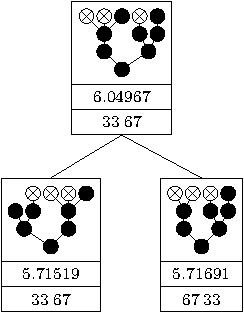
\includegraphics{p3/preemtive/0012233345_nonpreemtive.pdf}
    \caption{Optimal non-preemtive schedule.}
  \end{subfigure}
  \quad
  \begin{subfigure}{.45\linewidth}
    \centering
    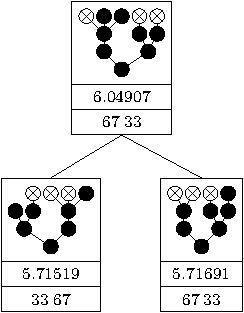
\includegraphics{p3/preemtive/0012233345_preemtive.pdf}
    \caption{A better preemtive schedule.}
  \end{subfigure}
  \caption{Preemtive vs. non-preemtive scheduling for $(0,0,1,1,1,2,2,2)$. Note that the snapshots in the second line are the same, but they are reached with different probabilities due to the fact that we can reschedule in the preemtive case.}
  \label{fig:preemtive-example-00111222}
\end{figure}

Another example that shows nicely that preemtive scheduling yields better results in some cases is the intree $(0,0,1,2,2,3,3,6,8,9,10,11,12,13)$ shown in figure \ref{fig:2-hlf-plus-one-not-optimal}. It is clear that -- if the first 6 steps, always the topmost task is the first task to finish, we at some point reach the intree shown in figure \ref{fig:preemtive-better-bad-case}. If we allowed to reschedule (by possibly interrupting the execution of some tasks) and chose a schedule as shown in figure \ref{fig:preemtive-better-good-case}, we would obviously acchieve a better overal run time. 

\begin{figure}[ht]
  \centering
  \begin{subfigure}{.46\textwidth}
    \centering
    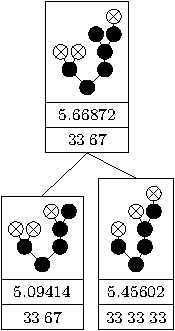
\includegraphics{p3/preemtive/00112556subopt.pdf}
    \caption{Suboptimal schedule. These snapshots are part of the optimal schedule for the intree $(0,0,0,2,3,4,5,7,7,9,10,10,12)$, shown in figure \ref{fig:2-hlf-plus-one-not-optimal}.}
    \label{fig:preemtive-better-bad-case}
  \end{subfigure}
  \quad
  \begin{subfigure}{.46\textwidth}
    \centering
    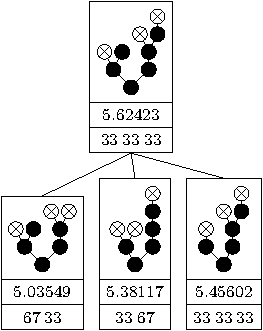
\includegraphics{p3/preemtive/00112556opt.pdf}
    \caption{Optimal schedule for $(0,0,1,1,2,5,5,6)$. This schedule is HLF.}
    \label{fig:preemtive-better-good-case}
  \end{subfigure}
  \caption{Intree $(0,0,1,1,2,5,5,6)$. This intree might result at some point from the intree $(0,0,1,2,2,3,3,6,8,9,10,11,12,13)$ with the two lowest tasks scheduled (see figure \ref{fig:2-hlf-plus-one-not-optimal}). If we allowed for preemting tasks we could improve the overal run time.}
  \label{fig:preemtive-is-better}
\end{figure}

\subsection{Considerations about subtrees}
\label{sec:properties-optimal-schedules-no-implications}

From another point of view, the intree $(0,0,1,2,2,3,3,6,8,9,10,11,12,13)$ shows that an optimal schedule may be forced at some time to process a subtree in a way that it would not process it if the subtree was processed for itself. This means that we can formulate the following:

\begin{theorem}
  There are intrees $T$ and $S$ such that $T$ is a subtree of $S$ and both $T$ and $S$ have the same root such that the optimal (non-preemtive) schedule for $S$ is HLF, but the optimal (non-preemtive) schedule for $T$ is non-HLF.
\end{theorem}

\begin{proof}
  See considerations above.
\end{proof}

\section{Size of the snapshot DAG}
\label{sec:p3-size-of-snapshot-dag-first-attempts}

Similar to the reasoning in section \ref{sec:p2-snapshot-dag}, we can research the size of a snapshot DAG for the P3 case. 
We conducted an experiment and examined the size for snapshot DAGs of intrees containing up to 17 tasks. 
Therefore, we generated all intrees (up to isomorphism) with a certain number of tasks (see section \ref{sec:enumerating-all-intrees} for an algorithm).
Then we computed the following for each intree:
\begin{itemize}
\item Number of distinct (i.e. non-isomorphic) subtrees.
\item Number of snapshots that can be constructed using the LEAF scheduling strategy (i.e. ``try-everything'' scheduling).
\item The size of the \emph{optimal} snapshot DAG.
\end{itemize}

We do so because of the following: It is easily possible to construct an optimal schedule if we take the possible snapshot DAGs of the LEAF scheduler and only leave the choices that yield the best expected run time.

Since the size of the snapshot DAG for an intree with $n$ tasks is at most $n^3$ times as large as the number of subtrees of the original intree, we also computed the number of subtrees for each of these intrees.
That is, we can compare the number of intrees to the number of snapshots to be considered.

The results are summed up in table \ref{tab:num-subtrees-size-of-dags}\todo{Complete!}.

\begin{table}[ht]
  \centering
  \begin{tabular}[ht]{ccccccc}
    \multirow{2}{*}{Tasks} & \multicolumn{2}{c}{Subtrees} & \multicolumn{2}{c}{Snapshots} & \multicolumn{2}{c}{``Optimal DAG''} \\
    & Max & Avg & Max & Avg & Max & Avg \\
    \hline
    3 & 3 & 3.00 & 3 & 3.00 & 3 & 3.00  \\
    4 & 5 & 4.25 & 5 & 4.25 & 5 & 4.25  \\
    5 & 7 & 5.89 & 7 & 5.89 & 7 & 5.89  \\
    6 & 11 & 8.10 & 11 & 8.25 & 11 & 8.05  \\
    7 & 16 & 11.04 & 19 & 11.75 & 16 & 10.81  \\
    8 & 24 &  15.10 & 34 & 17.39 & 22 & 14.37  \\
    9 & 34 &  20.57 & 63 & 26.53 & 31 & 18.76  \\
    10 & 54 &  28.08 & 119 & 41.85 & 41 & 24.16  \\
    11 & 79 &  38.33 & 230 & 67.48 & 55 & 30.67  \\
    12 & 119 & 52.41 & 437 & 112.68 & 71 & 38.41  \\
    13 & 169 &  71.69 & 812 & 184.95 & 89 & 47.49  \\
    14 & 269 &  98.19 & 1510 & 304.41 & 113 & 58.05  \\
    % 15 & 357 &  125.70 & 142 & 67.83  \\
    % 16 & 594 &  171.29 & 184 & 80.55  \\
    % 17 & 850 &  240.39 & 235 & 96.67  \\
  \end{tabular}
  \caption{Number of subtrees, size of the optimized snapshot DAG depending on the number of tasks. ``Subtrees'' denotes the number of distinct subtrees. ``Snapshots'' shows the number of distinct snapshots that have to be examined if we try all possible schedules. The column ``Optimal DAG'' shows the size of the snapshot DAG describing the optimal schedule.}
  \label{tab:num-subtrees-size-of-dags}
\end{table}

As we can see in table \ref{tab:num-subtrees-size-of-dags}, the number of subtrees is (at least for $n\geq  9$) significantly larger than the number of snapshots in the snapshot DAG describing an optimal schedule.

Another interesting fact is that there is no ``strict correlation'' between the number of subtrees and the number of snapshots in the optimal snapshot DAG. That is, there are certain DAGs that have more non-isomorphic subtrees than another DAG, yet -- on the other hand -- more snapshots in the optimal snapshot DAG. As an example, consider the intrees $T_1$ described by 00011111 and $T_2$ described by 00001234: $T_1$ has 19 subtrees and its optimal snapshot DAG contains 13 snapshots, while $T_2$ has only 15 subtrees, but an optimal snapshot DAG containing 14 snapshots.

Moreover, intrees containing $n$ tasks and having the maximal number of subtrees are (at least for $8\leq n \leq 17$) are not the ones having the largest optimal snapshot DAG.

To determine the maximum size of the optimal snapshot DAG for the P3 case, it might be useful to investigate whether the trees that have a large snapshot DAG can be constructed according to a specific pattern. The intrees resulting in snapshot DAGs of maximum size are depicted in figure \ref{fig:intrees-maximum-snapshot-dag-size-p3}. The intrees in this figure seem to behave quite chaotic and we were not able to deduce any pattern according to which they could be generated for general $n$.

\begin{figure}[t]
  \centering
  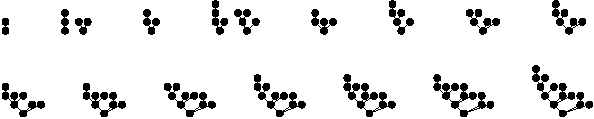
\includegraphics[scale=1.4]{p3/max_unoptimized.pdf}
  \caption{These are the intrees for which the a brute-force algorithm has to generate maximally many snapshots to generate the optimal schedule (maximal compared to all other intrees with the same number $n$ of vertices). We show $2\leq n \leq 14$.}
  \label{fig:intrees-maximum-unoptimized-p3}
\end{figure}

\begin{figure}[t]
  \centering
  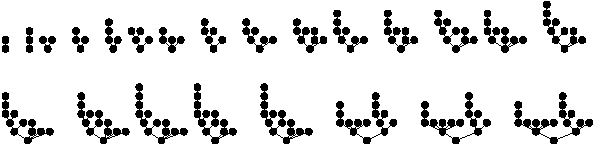
\includegraphics[scale=1.4]{p3/max_snapshot_dag.pdf}
  \caption{These intrees result in \emph{optimal} snapshot DAGs that are larger than all other optimal snapshot DAGs resulting from intrees having the same number of tasks $n$ ($2 \leq n \leq 17$ shown). There seems to be no simple pattern according to which these trees are constructed.}
  \label{fig:intrees-maximum-snapshot-dag-size-p3}
\end{figure}

% \section{Special classes of intrees}
% \label{sec:p3-dag-size-special-class-of-intrees}

% If we consider trees. whose sequence description is of the form $(0, 0, 1, 1, 3, 3, 5, 5, 7,7, 9,9,\dots)$, that have an even number of nodes, then the optimal snapshot DAGs have $\binom{n}{1}+\binom{n}{2}+\binom{n}{3}$ snapshots. \todo{Make this conjecture and nice!}

% \begin{table}[ht]
%   \centering
%   \begin{tabular}{lcc}
%     Class & No. snaps & Opt. size \\
%     $(0,0,1,1,3,3,5,5,\dots)$ & & $\binom{n/2}{1}+\binom{n/2}{2}+\binom{n/2}{3}$ \\
%     $(0,0,0,1,1,1,4,4,4,7,7,7,\dots)$ & & $((n/3)^3 + 2*(n/3))/3$
%   \end{tabular}
%   \caption{Classes and their DAG sizes}
%   \label{tab:special-classes-dag-sizes}
% \end{table}

\section{Degenerate intrees}
\label{sec:p3-degenerate-intrees}

\todo{Definitions: intree, level, suc, adding tasks to trees etc.}

We now focus one one particular class on intrees, namely \emph{degenerate intrees}. A degenerate intree is an intree that consists of one longest chain from the bottom to one leaf, and all other tasks are direct predecessors to one of the tasks within this longest chain. Another characterization is the following: On each level, \emph{at most one task} has predecessors.\todo{Figure zeigen.}

\subsection{Intro: Degenerate binary trees}
\label{sec:p3-degenerate-trees-binary}

We researched degenerate binary trees, i.e. trees whose sequence has the structure
\begin{equation*}
  \left( 0,0,a_0,a_1,a_2,a_3,a_4,\dots,a_n \right),
\end{equation*}
for $n+3$ the total number of tasks within the intree. The values $a_i$ can be recursively defined as follows:
\begin{equation*}
  a_k =
  \begin{cases}
    1, & \text{if } k\leq 1 \\
    a_{k-1}, & \text{if } k>1 \text{ is odd} \\
    a_{k-1}+2, & \text{if } k>1 \text{ is even}
  \end{cases}
\end{equation*}

That is, degenerate binary trees have sequences of the form $(0,0,1,1,3,3,5,5,7,7,9,\dots)$.

We now examine how many snapshots are considered if we compute the optimal P3 schedule by considering \emph{all} possibilities and afterwards discarding the bad ones. The results are summed up in table \ref{tab:p3-degenerate-binary-trees-no-snapshots}. We clearly observe that the number of snapshots grows exponentially (at least within the range for $n$ under consideration). A simple pattern that can be observed from table \ref{tab:p3-degenerate-binary-trees-no-snapshots} is that (at least for $n\leq 26$) that the number of snapshots for a degenerate binary tree with $n$ tasks is greater than twice the number of snapshots for a degenerate binary tree with $n-2$ tasks. If $S(n)$ denotes the number of snapshots for a degenerate binary tree, we can formulate $S(n)>S(n-2)$, which we can (by induction) convert to $S(n) > \sqrt 2 ^ n$.

This can be illustrated by the fact that degenerate binary intrees are fully determined by their profile (please see section \ref{sec:p2-profiles} for the definition of profiles). A degenerate binary tree has a profile of the form
\begin{equation*}
  \profile{a,2,2,2,2,\dots,2,1},
\end{equation*}
where $a$ is either $1$ or $2$. Assume the length of the profile (i.e. the height of the degenerate binary tree) is exactly $l$. Then, we have $2\cdot(l-2)+1+a = 2l-1+a$ tasks in total. Assume for now that $a=2$ (i.e. we are dealing with a complete degenerate binary tree) and $l>2$.

A subtree of a this degenerate binary intree having height $l'$ has a profile of the form
\begin{equation*}
  \profile{a_0,a_1,a_2,\dots,a_{l'-2},1},
\end{equation*}
where $1\leq a_0\leq a$ and $1\leq a_i \leq 2$ for all $i\in\left\{ 1,2,\dots,l-2 \right\}$. Using basic combinatorics, we can tell that there must be
\begin{equation*}
  \sum_{l'=0}^{l-1} 2^{l'} = 2^{l} -1
\end{equation*}
distinct subtrees if $a=2$ for profile length (resp. intree depth) $l$.

If $a=1$ and we have a profile length of $l$, we cann argue that there must be as many subtrees as for the profile without the first item (then of length $l-1$) plus the number of profiles of length exactly $l-1$ with one additional 1 prepended. These are exactly $2^{l-2}$.

This, in total leads to our desired bound for $S(n)$.\todo{Genauer machen.}

\begin{table}[t]
  \centering
  \begin{tabular}[ht]{ccc}
    \multirow{2}{*}{Tasks} & \multicolumn{2}{c}{Snapshots} \\
    & Overall & HLF \\
    \hline
    3  &  3       & 3   \\
    4  &  5       & 5   \\
    5  &  7       & 7   \\
    6  &  11      & 11  \\
    7  &  17      & 14  \\
    8  &  28      & 21  \\
    9  &  48      & 25  \\
    10 &  85      & 36  \\
  \end{tabular}
  \begin{tabular}[ht]{ccc}
    \multirow{2}{*}{Tasks} & \multicolumn{2}{c}{Snapshots} \\
    & Overall & HLF \\
    \hline
    11 &  150     & 41  \\
    12 &  276     & 57  \\
    13 &  477     & 63  \\
    14 &  884     & 85  \\
    15 &  1477    & 92  \\
    16 &  2717    & 121 \\
    17 &  4398    & 129 \\
    18 &  7991    & 166 \\
  \end{tabular}
  \begin{tabular}[ht]{ccc}
    \multirow{2}{*}{Tasks} & \multicolumn{2}{c}{Snapshots} \\
    & Overall & HLF \\
    \hline
    19 &  12600   & 175 \\
    20 &  22594   & 221 \\
    21 &  34883   & 231 \\
    22 &  61774   & 287 \\
    23 &  93775   & 298 \\
    24 &  164187  & 365 \\
    25 &  245852  & 377 \\
    26 &  426089  & 456 \\
  \end{tabular}
  \caption{Number of snapshots for degenerate binary trees in the P3 case. The first column shows the number of tasks. ``Overall'' denotes the number of distinct snapshots that are explored if an optimal schedule is constructed by examining all schedulings. ``HLF'' denotes the number of distinct snapshots for HLF.}
  \label{tab:p3-degenerate-binary-trees-no-snapshots}
\end{table}

Interestingly, degenerate binary intrees, while having a possibly huge amount of snapshots, are probably optimally scheduled by HLF. You can compare the number of HLF snapshots to the number of overal snapshots by looking at table \ref{tab:p3-degenerate-binary-trees-no-snapshots}.

We generalize this fact in the next section.

\subsection{HLF is optimal for degenerate intrees}
\label{sec:p3-degenerate-intrees-hlf-optimal}

\begin{lemma}
  \label{lem:p3-adding-tasks-level-keep-scheduled-same-inequality}
  Let $I$ be a degenerate intree and $x, y$ two (not necessarily distinct) ready tasks within this intree. Let $z_1, z_2$ be two new tasks that will be added to this intree with $level(z_1) > level(z_2)$ in a manner such that $I_1:=I\cup\left\{ z_1 \right\}$ and $I_2:=I\cup\left\{ z_2 \right\}$ are still degenerate intrees. Moreover, the tasks $z_1$ and $z_2$ shall be added in such a way that neither $x$ nor $y$ is a successor of $z_1$ or $z_2$ (i.e. $x,y$ stay ready in $I_1$ resp. $I_2$). 
  
  By $T^*_{t_1,t_2,t_3}(I)$ we denote the optimal expected run time that can be acchieved if we \emph{initially} schedule all tasks from the set $\left\{ t_1,t_2,t_3 \right\}$. \todo{Notation auslagern.} Note that this notation does not necessarily require that we actually have three tasks (e.g. if $t_1=t_2$).
  
  Then, if $x,y$ and $z_1$ resp. $z_2$ are used as initial tasks, we have the following for the best acchievable expected run times (for respective initial tasks):
  \begin{equation}
    \label{eq:lemma-p3-adding-tasks-level-keep-scheduled-same-inequality}
    T^{*}_{x,y,z_1}\left(I\cup\left\{ z_1 \right\}\right) > T^{*}_{x,y,z_2}\left( I\cup\left\{ z_2 \right\} \right)
  \end{equation}

  If we loosen the level condition to $level(z_1)\geq level(z_2)$, we obtain
  \begin{equation*}
    T^{*}_{x,y,z_1}\left(I\cup\left\{ z_1 \right\}\right) \geq T^{*}_{x,y,z_2}\left( I\cup\left\{ z_2 \right\} \right).
  \end{equation*}
\end{lemma}

\begin{proof}
  We focus first on the case where $level(z_1) > level(z_2)$ and prove the claim by induction over the number of nodes:
  
  The induction basis is the case where we have degenerate intrees with 3 tasks\footnote{We start by 3 tasks since these trees are the only ones that allow adding $z_1$ and $z_2$ at different levels such that both $x$ and $y$ stay ready. For an intree with two tasks, the claim can be seen by simply examining that $T(0,0)<T(0,1)$\todo{Improve this footnote.}.} (all of them are depicted in figure \ref{fig:p3-lemma-adding-intrees-induction-start} (only the black nodes)).
  
  \begin{figure}[t]
    \centering
    \begin{tikzpicture}[scale=0.25]
      \newcommand{\treeone}{
        \fill(0,0) circle (0.4);
        \fill(0,1) circle (0.4);
        \fill(0,2) circle (0.4);
        \draw(0,0) -- (0,1);
        \draw(0,1) -- (0,2);
      }
      \newcommand{\treetwo}{
        \fill(0,0) circle (0.4);
        \fill(-.50,1) circle (0.4);
        \fill(.50,1) circle (0.4);
        \draw(0,0) -- (0.5,1);
        \draw(0,0) -- (-.5,1);
      }
      \newcommand{\treethree}{
        \fill(0,0) circle (0.4);
        \fill(0,1) circle (0.4);
        \draw(0,0) -- (0,1);
      }
      % \begin{scope}
      %   \treeone;
      % \end{scope}
      % \begin{scope}[xshift=9cm]
      %   \treetwo;
      % \end{scope}

      \begin{scope}[yshift=-5cm, xshift=-20.5cm]
        \begin{scope}
          \treethree;
          \draw(0,1) -- (0,2);
          \draw[fill=white](0,2) circle (0.4);
          \node at (0,-2) {3};
        \end{scope}
        \node at (2.5,-2) {$>$};
        \begin{scope}[xshift=5cm]
          \treethree;
          \draw(0,0) -- (1,1);
          \draw[fill=white](1,1) circle (0.4);
          \node at (0,-2) {2.5};
        \end{scope}
      \end{scope}

      \begin{scope}[yshift=-5cm, xshift=-3.5cm]
        \begin{scope}
          \treeone;
          \draw(0,2) -- (0,3);
          \draw[fill=white](0,3) circle (0.4);
          \node at (0,-2) {4};
        \end{scope}
        \node at (2.5,-2) {$>$};
        \begin{scope}[xshift=5cm]
          \treeone;
          \draw(0,1) -- (1,2);
          \draw[fill=white](1,2) circle (0.4);
          \node at (0,-2) {3.5};
        \end{scope}
        \node at (8,-2) {$>$};
        \begin{scope}[xshift=11cm]
          \treeone;
          \draw(0,0) -- (1,1);
          \draw[fill=white](1,1) circle (0.4);
          \node at (0,-2) {3.25};
        \end{scope}
        % \node at (4,-1.5) {$4 > 3.5 > 3.25$};
      \end{scope}

      \begin{scope}[yshift=-5cm, xshift=20cm]
        \begin{scope}[xshift=0cm]
          \treetwo;
          \draw(-.5,1) -- (-.5,2);
          \draw[fill=white](-.5,2) circle (0.4);
          \node at (0,-2) {3.25};
        \end{scope}
        \node at (2.5,-2) {$>$};
        \begin{scope}[xshift=5cm]
          \treetwo;
          \draw(0,0) -- (1.5,1);
          \draw[fill=white](1.5,1) circle (0.4);
          \node at (0,-2) {2.83};
        \end{scope}
      \end{scope}
      
    \end{tikzpicture}
    \caption{Adding new tasks to degenerate intrees with less than four nodes such that the resulting intrees are still degenerate. The original (2- resp. 3-node) intrees are drawn black, the newly added tasks are drawn white. Below each intree, we see the corresponding optimal expected run time. The lower the level of the newly added task, the lower the expected run time. This serves as basis for the induction proof for lemma \ref{lem:p3-adding-tasks-level-keep-scheduled-same-inequality}.}
    \label{fig:p3-lemma-adding-intrees-induction-start}
  \end{figure}

  If we add two tasks $z_1$ and $z_2$ with $level(z_1)>level(z_2)$ in a way such that the original ready tasks stay ready and the resulting intrees stay degenerate, we obtain the intrees depicted in figure \ref{fig:p3-lemma-adding-intrees-induction-start} (trees \emph{including} the white nodes). By simply computing the expected optimal run times, we can confirm our claim for intrees with 3 nodes.

  We now do the induction step by considering an intree with $n$ tasks. 
  Let $x,y$ be ready tasks and $z_1$ and $z_2$ to be added with $level(z_1) > level(z_2)$ such that the resulting intrees are degenerate.
  We can now compare the two runs that can occur if $x,y,z_1$ resp. $x,y,z_2$ are initially scheduled. 
  Therefore, we consider what happens in $I_1=I\cup\left\{ z_1 \right\}$ resp. $I_2=I\cup\left\{ z_2 \right\}$ if either $x$, $y$ or $z_1/z_2$ finishes first:

  \begin{itemize}
  \item If $z_1$ resp. $z_2$ is the first task to finish, the resulting intree is exactly $I$. Thus, the remaining run times for these cases are identical if the next task chosen is the same in both trees. We denote the task that may be chosen additionally to $x$ and $y$ by $z'$. If it is the case that only $x$ and $y$ can be scheduled, we set $z'=x$ to simplify notation. The corresponding run time for the resulting intree is then $T^*_{x,y,z'}(I)$.

  \item If $x$ is the first task to finish, then the resulting intrees are 
    \begin{equation*}
      I^x_{1}=I_1\setminus\left\{ x \right\} \quad \text{ resp. } \quad I^x_{2}=I_2\setminus\left\{ x \right\}.
    \end{equation*}

    By $x'$ we denote the task that is scheduled next in the optimal schedule for intree $I_1^x$. 
    If there are only two ready tasks left in $I_1^x$ (which then must be $y$ and $z_1$), we set $x'=y$. The expected optimal runtime for $I_1^x$ in this situaion is then given by $T_{x',y,z_1}^*(I_1^x)$.

    We now examine whether $x'$ is also ready in the intree $I_2^x$:
    \begin{itemize}
    \item If there are only two ready tasks left in $I_1$ (namely $x$ and $y$), we set -- as mentioned before -- $x'=y$. Thus, in $I_2^x$, $x'$ is still ready\footnote{It may even be the case that $I_2^x$ contains some additional ready tasks that are not ready in $I_1^x$.}.
    \item If $x'$ is the direct successor of $x$, then $x$ must have been the \emph{single topmost task} and the \emph{single predecessor} of $x'$ (since $I_1^x$ is a degenerate tree). However, since we assumed that $level(z_2)<level(z_1)$ and $z_1$ can not be a predecessor of $x'$ (since $x'$ is ready in $I_1$), it can not be the case that $z_2$ blocks $x'$ in $I_2^x$. We conclude that in this case $x'$ is ready in $I_2^x$.

      % Moreover, since $x'$ is ready in $I_1^x$, the task $z_1$ can not be a predecessor of $x'$. Since $level(z_2)<level(z_1)$ and since $I_1^x$ and $I_2^x$ are both degenerate intrees, $z_2$ can not block $x'$.\todo{Genauer ausführen. Evtl. auslagern.}
    \item If $x'$ is not the direct successor of $x$, we recognize the fact that $x'$ must reside on a certain level with in the degenerate intree. 

      If $x'$ is \emph{not} in the topmost level, it can not be blocked by $z_2$ because we assumed that $z_2$ is added in a way such that $I\cup\{z_2\}$ is still a degenerate intree.

      Otherwise (if $x'$ is a topmost task), $z_2$ can not be added \emph{above} $x'$ because we assumed $level(z_1)>level(z_2)$.

      Again, $x'$ is ready in $I_2^x$.
      % we still have two subcases:
      % \begin{itemize}
      % \item If there are other tasks at the same level as $x'$ (i.e. at the topmost level), then we can -- without loss of generality\footnote{Because of isomorphism.} -- assume that $z_2$ was added to another task on the same level as $x'$.
      % \item If $x'$ was the \emph{only} topmost task, then it \emph{might} be the case that $z_2$ was chosen in a way such that it is the direct predecessor of $x'$. In this case, we can argue that $level(z_1) > level(z_2)$ and, thus, know that $z_2$ can not block $x'$, because $x'$ is a topmost task.
      % \end{itemize}

      % $x'$ must be on a lower level then $x$ (because we are dealing with a degenerate intree). We assumed that we added $z_2$ in a manner such that $I_2=I\cup\left\{ z_2 \right\}$ is a degenerate subtree. Thus, $z_2$ could not have been added with $x'$ as its successor. Thus, $x'$ is not blocked by $z_2$ in $I_2$.
    \end{itemize}
    We observed that for $I_2^x$, the task $x'$ must be ready.
    
    The intrees $I^x_{1}$ and $I^x_{2}$ have exactly $n$ tasks -- and they have a common subtree, namely
    \begin{equation*}
      I^x := I^x_{1}\setminus\left\{ z_1 \right\}=I^x_{2}\setminus\left\{ z_2 \right\}.
    \end{equation*}

    
    We can now apply the induction hypothesis for the intree $I^x$, since this intree contains only $n-1$ tasks: We have an intree with $n-1$ tasks (namely $I^x$) and two tasks $z_1$ and $z_2$ with $level(z_1)>level(z_2)$, $I^x_1 = I^x\cup\left\{ z_1 \right\}$ and $I^x_2 = I^x\cup\left\{ z_2 \right\}$, implying that $T^*_{x',y,z_1}(I^x_1)>T^*_{x',y,z_2}(I^x_{2})$.
  \item If $y$ is the first task to finish, we argue similar to the $x$ case, thereby considering $I^y_{1},I^y_{2}$ and $I^y$ which are all defined analogously. This finally yields the following inequality: $T^*_{x,y',z_1}(I^y_{1}) > T^*_{x,y',z_2}(I^y_{2})$.
  \end{itemize}

  The above considerations are illustrated in figure 
\ref{fig:p3-adding-tasks-level-keep-scheduled-same-inequality}.\todo{Figure anpassen!}
  
  \begin{figure}[t]
    \centering
    \newcommand{\drawx}{
      \node[draw=black,circle] at (.9,3) {$x$};
    }
    \newcommand{\drawxx}{
      \node[draw=black,circle] at (.7,2) {$x'$};
    }
    \newcommand{\drawy}{
      \node[draw=black,circle] at (-1.5,4) {$y$};
    }
    \newcommand{\drawyy}{
      \node[draw=black,circle] at (-1.5,3) {$y'$};
    }
    \newcommand{\rawtriangle}{
      \draw
      [dotted, very thick,
      %fill=white!90!black, 
      rounded corners]
      (0,0) -- (3,2) -- (3.5,8) -- (-3.5,8) -- (-3,2) -- cycle;
    }
    \newcommand{\treetriangle}{
      \rawtriangle;
      \drawx;
      \drawy;
    }
    \newcommand{\abstand}{7.5cm}
    \begin{tikzpicture}[scale=.4]
      \begin{scope}[xshift=-\abstand]
        \treetriangle
        \node[draw=black,circle] at (0,6.5) {$z_1$};
      \end{scope}
      \begin{scope}[xshift=\abstand]
        \treetriangle
        \node[draw=black,circle] at (1,5) {$z_2$};
      \end{scope}
      
      \begin{scope}[xshift=-2*\abstand, yshift=-9cm]
        \rawtriangle
        \node[draw=black,circle] at (0,6.5) {$z_1$};
        \drawxx;
        \drawy;
      \end{scope}

      \begin{scope}[xshift=-\abstand, yshift=-9cm]
        \rawtriangle
        \node[draw=black,circle] at (0,6.5) {$z_1$};
        \drawx;
        \drawyy;
      \end{scope}

      \begin{scope}[xshift=0, yshift=-9cm]
        \treetriangle
        \node[draw=black,circle] at (.3,5.5) {$z'$};
      \end{scope}
      
      \begin{scope}[xshift=\abstand, yshift=-9cm]
        \rawtriangle
        \node[draw=black,circle] at (1,5) {$z_2$};
        \drawxx;
        \drawy;
      \end{scope}

      \begin{scope}[xshift=2*\abstand, yshift=-9cm]
        \rawtriangle
        \node[draw=black,circle] at (1,5) {$z_2$};
        \drawx;
        \drawyy;
      \end{scope}
      
      \draw[thick,->](-\abstand,0) -- +(0,-.8);
      \draw[thick,->](-\abstand-2cm,1) -- +(-\abstand+4cm,-1.6);
      \draw[thick,->](-\abstand+2cm,1) -- +(\abstand-4cm,-1.6);

      \begin{scope}[xshift=2*\abstand]
        \draw[thick,->](-\abstand,0) -- +(0,-.8);
        \draw[thick,->](-\abstand-2cm,1) -- +(-\abstand+4cm,-1.6);
        \draw[thick,->](-\abstand+2cm,1) -- +(\abstand-4cm,-1.6);
      \end{scope}
      
      % legend      
      \draw[decoration=brace,decorate=true](-11,8.25) --node[above]{$I_1$} +(7,0);
      \draw[decoration=brace,decorate=true](  4,8.25) --node[above]{$I_2$} +(7,0);
      \draw[decoration={brace,mirror},decorate=true](  -18,-9.5) --node[below, yshift=-.2cm]{$I^x_{1}$} +(6,0);
      \draw[decoration={brace,mirror},decorate=true](-10.5,-9.5) --node[below, yshift=-.2cm]{$I^y_{1}$} +(6,0);
      \draw[decoration={brace,mirror},decorate=true](   -3,-9.5) --node[below, yshift=-.2cm]{$I$} +(6,0);
      \draw[decoration={brace,mirror},decorate=true](  4.5,-9.5) --node[below, yshift=-.2cm]{$I^x_{2}$} +(6,0);
      \draw[decoration={brace,mirror},decorate=true](   12,-9.5) --node[below, yshift=-.2cm]{$I^y_{2}$} +(6,0);
    \end{tikzpicture}

    \caption{Proof sketch for lemma \ref{lem:p3-adding-tasks-level-keep-scheduled-same-inequality}. By induction hypothesis, we have that $T^*_{x',y,z_1}(I^x_{1}) > T^*_{x',y,z_2}(I^x_{2})$ and $T^*_{x,y',z_1}(I^y_{1}) > T^*_{x,y',z_2}(I^y_{2})$, from which we deduce $T^*_{x,y,z_1}(I_1) > T^*_{x,y,z_2}(I_2)$. Note that $z_2$ can not block $x'$ or $y'$ since $z_1$ didn't block any of the two and we required that adding $z_1$ resp. $z_2$ still results a degenerate tree.}
    \label{fig:p3-adding-tasks-level-keep-scheduled-same-inequality}
  \end{figure}
  
  Now we argue that the run times for $I_1$ and $I_2$ can be computed as follows:
  \begin{align*}
    T^*_{x,y,z_1}(I_1) & = 
      \frac{1}{3} + 
      \frac{1}{3}\cdot \left( 
        T_{x,y,z'}^*(I) + 
        T^*_{x',y,z_1}(I^x_{1}) +
        T^*_{x,y',z_1}(I^y_{1}) 
      \right)
      \\
    T^*_{x,y,z_2}(I_2) & = 
      \frac{1}{3} + 
      \frac{1}{3}\cdot \left( 
        T_{x,y,z'}^*(I) + 
        T^*_{x',y,z_2}(I^x_{2}) +
        T^*_{x,y',z_2}(I^y_{2}) 
      \right)
  \end{align*}

  We will now use the aforementioned inequalities $T^*_{x',y,z_1}(I^x_{1}) > T^*_{x',y,z_2}(I^x_{2})$ and $T^*_{x,y',z_1}(I^y_{1}) > T^*_{x,y',z_2}(I^y_{2})$:
\begin{align*}
    T^*_{x,y,z_1}(I_1) & = 
      \frac{1}{3} + 
      \frac{1}{3}\cdot \left( 
        T_{x,y,z'}^*(I) + 
        T^*_{x',y,z_1}(I^x_{1}) +
        T^*_{x,y',z_1}(I^y_{1}) 
      \right)
      > 
      \\
      & >
      \frac{1}{3} + 
      \frac{1}{3}\cdot \left( 
        T_{x,y,z'}^*(I) + 
        T^*_{x',y,z_2}(I^x_{2}) +
        T^*_{x,y',z_2}(I^y_{2}) 
      \right) 
      = T^*_{x,y,z_2}(I_2).
  \end{align*}

  This proves our claim for $level(z_1) > level(z_2)$. It is simple to obtain the claim for the version where $level(z_1) \geq level(z_2)$: If the levels are the same, the resulting degenerate intrees $I_1$ and $I_2$ are isomorphic (and there is an isomorphism that maps $z_1$ onto $z_2$), thus the optimal run time is the same. If the levels are different, we argument as in the beginning of the proof.
\end{proof}

\paragraph{Application of lemma \ref{lem:p3-adding-tasks-level-keep-scheduled-same-inequality}}

We presented lemma \ref{lem:p3-adding-tasks-level-keep-scheduled-same-inequality} in a way that involved adding tasks to a certain intree, because this related well to our proof technique. In practice, we can use it to compare two degenerate intrees with $n$ nodes and that have a common subtree containing $n-1$ nodes.

We can now derive the following theorem.

\begin{theorem}
  Degenerate intrees are optimally scheduled by HLF.
\end{theorem}

\begin{proof}
  Consider a degenerate intree with $n=3$ tasks. It is trivially clear that for P3, a HLF schedule is optimal for this intree (see figure \ref{fig:p3-lemma-adding-intrees-induction-start} to see what these intrees look like -- we simply can conclude examine all possible schedules and see that the optimal ones is exactly HLF).
  
  Consider now a degenerate tree $I$ with $n$ nodes and assume that we know that for all degenerate trees with $n-1$ nodes HLF is optimal for three processors. If $I$ has two or less topmost tasks, it is obvious that we have to use HLF (since we can use at most two processors and HLF is known to be optimal for two processors --- see chapter \ref{chap:p2}).

  Thus, we only have to focus on the case where $I$ has at least three ready tasks.

  If we choose three topmost tasks $x,y,z$ of $I$, we can argue as follows: If $x$ is the task that finishes first, for the resulting subtree $I\setminus \left\{ x \right\}$, we can be sure that we can choose the next task such that we adhere to HLF, thus choosing the optimal solution for $I\setminus\left\{ x \right\}$ (by induction hypothesis). The same holds if $y$ or $z$ finishes first.
  
  We now consider a (possibly) non-HLF schedule for $I$ and compare it to the HLF schedule described before.
  Let $x',y',z'$ be the tasks to be chosen such that at least $x\neq x'$ or $y\neq y'$ or $z\neq z'$. We can -- without loss of generality -- assume $level(x')\leq level(x)$, $level(y')\leq level(y')$, $level(z')\leq level(z)$. If $x'$ is the first task to finish, we consider the degenerate intree $I\setminus\left\{ x' \right\}$. Since $I \setminus \left\{ x' \right\}$ is a degenerate intree with $n-1$ tasks, it would be optimal to use HLF. However, using HLF may or may not be possible depending on our previous choices of $y'$ and $z'$. That is, the optimum for $I\setminus\left\{ x' \right\}$ \emph{might} be acchieved if we chose $y'$ and $z'$ accordingly. From this we can conclude that the optimal expected run time is at least $T_{HLF}\left( I\setminus\left\{ x' \right\} \right)$, where $T_{HLF}$ denotes the run time for HLF (which we know, by induction, is optimal).

  Now we compare the run time for $I\setminus\left\{ x' \right\}$ to the optimal run time for $I \setminus\left\{ x \right\}$, which is exactly given by $T_{HLF}\left( I \setminus\left\{ x \right\} \right)$. We recognize that $I\setminus\left\{ x' \right\}$ and $I\setminus\left\{ x \right\}$ have a common subtree, namely $I\setminus\left\{ x,x' \right\}$ with $n-2$ tasks.
  
  Moreover, we know that for both $I\setminus\left\{ x \right\}$ and $I\setminus\left\{ x' \right\}$ HLF is optimal (because of our induction hypothesis) and that for $I\setminus\left\{ x \right\}$ and $I\setminus\left\{ x' \right\}$ both $y$ and $z$ must be in the optimal (i.e. HLF) schedule since $y$ and $z$ are two of the three topmost tasks. At last, we have $level(x) \geq level(x')$.
  Thus, we can apply lemma \ref{lem:p3-adding-tasks-level-keep-scheduled-same-inequality} for the degenerate tree $I\setminus \{x,x'\}$ with tasks $y$ and $z$ and deduce that
  \begin{equation*}
    T_{x',y,z}(I\setminus\{x\}) 
    \leq 
    \underbrace{T_{x,y,z}(I\setminus\{x'\})}_{\text{Optimal for $I\setminus \{x'\}$}}.
  \end{equation*}
  Equality holds if $x$ and $x'$ are on the same level.

  As stated before, for the intree $I\setminus\{x'\}$, the schedule chosen \emph{might} be a non-HLF schedule. In this case, the schedule performs even worse than $T_{x,y,z}(I\setminus\{ x'  \})$, since the optimal schedule would choose $x,y,z$ as scheduled tasks. This means that
  \begin{equation*}
    T_{x,y,z}(I\setminus\{x'\})
    \leq
    T_{x'',y',z'}(I\setminus\{x'\}),
  \end{equation*}
  where $x''$ is the task chosen by the non-HLF schedule, finally implying (by $T_{HLF}(I\setminus\{x\}) \leq T_{x',y,z}\left( I\setminus\left\{ x \right\} \right)$) that
  \begin{equation*}
    T_{HLF}(I\setminus\{x\})
    \leq
    T_{x'',y',z'}(I\setminus\{x'\}).
  \end{equation*}
  %because the HLF schedule is at least as good as the schedule that starts out with tasks $x',y,z$.
  We argue similar for tasks $y$ and $y'$ resp. $z$ and $z'$ and finally obtain the following:

  \begin{eqnarray*}
    T_{x',y,z}(I\setminus\{x\})
    & \leq &
    T_{x'',y',z'}(I\setminus\{x'\}) \\
    T_{x,y',z}(I\setminus\{y\})
    & \leq &
    T_{x',y'',z'}(I\setminus\{y'\}) \\
    T_{x,y,z'}(I\setminus\{z\})
    & \leq &
    T_{x',y',z''}(I\setminus\{z'\}) \\
  \end{eqnarray*}
  Note that if e.g. $x=x'$, the above three equations are still satisfied.
  Combining the above inequalities yields that
  \begin{eqnarray*}
    %T_{HLF}(I) = 
    T_{x,y,z}(I) 
    & \leq & 
    \frac{1}{3} + \frac{1}{3} \cdot 
    \left( 
      T_{x',y,z}(I\setminus\{x\}) +
      T_{x,y',z}(I\setminus\{y\}) +
      T_{x,y,z'}(I\setminus\{z\})
    \right) 
    \leq \\
    & \leq &
    \frac{1}{3} + \frac{1}{3} \cdot 
    \left( 
      T_{x'',y',z'}(I\setminus\{x'\}) +
      T_{x',y'',z'}(I\setminus\{y'\}) +
      T_{x',y',z''}(I\setminus\{z'\})
    \right) \leq \\
    & \leq &
    T_{x',y',z'}(I)
  \end{eqnarray*}

  This finally shows that a HLF schedule is at least as good as an arbitrary other task, meaning that HLF is optimal for three processors on degenerate trees.
\end{proof}

\section{Parallel chains}
\label{sec:p3-parallel-chains}

We will now consider another class of intrees that can be shown to have HLF as optimal schedules.

\begin{definition}[Parallel chain]
  Let $I$ be an intree. We call $I$ a \emph{parallel chain}, if each task except the root has at most one predecessor. The root may have arbitrarily many predecessors.
\end{definition}

\todo{Figure von einer parallel chain.}

We start out by a lemma that we will use later. This lemma is an analogue variant of a lemma described in \cite{chandyreynoldsshortpaper1975}. While their lemma works for two processors and general intrees, our variant is for three processors, but restricted to parallel chains.

\begin{lemma}
  \label{lemma:parallel-chains-flatness}
  Let $I$ be an intree and $x$ and $y$ two ready tasks with $level(x) > level(y)$. Then, $T_{HLF}(I\setminus\{ x \}) < T_{HLF}(I\setminus\{ y \})$, where $T_{HLF}(I)$ denotes the run time that is acchieved if intree $I$ is scheduled according to HLF.
\end{lemma}

\begin{proof}
  \newcommand{\iminus}[1]{I\setminus\{#1\}}

  \todo{Induktionsanfang}

  We consider the HLF schedules on the intrees $I\setminus \{x\}$ and $I \setminus \{y\}$, with variable names as aforementioned. Note that the intrees $I\setminus \{x\}$ and $\setminus \{y\}$ have at least two common HLF-tasks (i.e. tasks that are scheduled by HLF). We call these two tasks $x_1$ and $x_2$. \todo{Erklären, was passiert, wenn es im nächsten Schritt nicht mehr drei, sondern weniger Tasks zur Verfügung gibt.}For the intree $\iminus{x}$, we call the third HLF-task $x_3$ and can compute its expected run time (for HLF) by
  \begin{equation*}
    T_{HLF}(\iminus{x}) = 
    \frac{1}{3} \cdot T(\iminus{x, x_1}) +
    \frac{1}{3} \cdot T(\iminus{x, x_2}) +
    \frac{1}{3} \cdot T(\iminus{x, x_3})
    .
  \end{equation*}
  On the other hand, for the intree $\iminus{y}$, we call the third HLF-task $x'$ and can compute its expected run time analogously by
  \begin{equation*}
    T_{HLF}(\iminus{y}) = 
    \frac{1}{3} \cdot T(\iminus{y, x_1}) +
    \frac{1}{3} \cdot T(\iminus{y, x_2}) +
    \frac{1}{3} \cdot T(\iminus{y, x'})
    .
  \end{equation*}
  We can now compare $T(\iminus{x, x_1})$ with $T(\iminus{y, x_1})$, $T(\iminus{x, x_2})$ with $T(\iminus{x, x_2})$ and $T(\iminus{x, x_3})$ with $T(\iminus{y, x'})$.
  
  The intrees $\iminus{x,x_1}$ and $\iminus{y,x_1}$ have a common subtree, namely $\iminus{x_1}$. By induction ($\iminus{x_1}$ has $n-1$ tasks, $level(x) > level(y)$), we know that the expected HLF run time for $\iminus{x,x_1}$ is less than the expected run time for $\iminus{y,x_1}$. Note that $\iminus{x, x_1}$ has at least as many ready tasks as $\iminus{y,x_1}$. So, if $\iminus{y,x_1}$ has two or less ready tasks, the claim is true, because it has been shown for two processors in \cite{chandyreynoldsshortpaper1975} and we -- moreover -- can use a third processor for$\iminus{x,x_1}$. This consideration can be done for $x_2$ in the same manner. 

  It remains to compare $T(\iminus{x, x_3})$ and $T(\iminus{y, x'})$. If $\iminus{y,x'}$ has fewer ready tasks than $T(\iminus{x, x_3})$, then we trivially have $T(\iminus{x, x_3}) \leq T(\iminus{y, x'})$ (similar to the case before, it has been shown for two processors, and we additionally can use a third processor for $\iminus{x,x_3}$). We, thus, focus on other cases.

  \begin{itemize}
  \item  If $level(x')=level(x_3)$, the intrees $\iminus{x'}$ and $\iminus{x_3}$ are isomorphic (we are dealing with parallel chains only), and can -- thus -- be considered equal in our computations. That is, we can w.l.o.g. assume $x'=x_3$ if the levels of $x'$ and $x_3$ are equal. In this case, we have that $T(\iminus{x, x_3})$ and $T(\iminus{y, x'})$ share a common supertree (namely $\iminus{x_3}=\iminus{x'}$), and we know -- by induction since $level(x)>level(y)$ that $T(\iminus{x, x_3}) < T(\iminus{y, x'})$.
  \item   If $level(x') \neq level(x_3)$, we know that $x_3$ is \emph{not} a HLF task in $\iminus{y}$, but $x'$ is. This means that $x'$ can only be a HLF task since it is not part of $\iminus{y}$. Therefore, we conclude that $y$ must be the same as $x_3$ (implying w.l.o.g. $\iminus{x,y}=\iminus{y,x'}$). This means that $level(x)>level(y)=level(x_3)$. Moreover, because $x'$ is only a HLF task because $x_3$ is not existent in $\iminus{y}$, we know that $level(x') < level(x_3)$. Combining the inequalities yields $level(x)>level(x')$. We can now argue that $\iminus{y}$ is (w.l.o.g.) a common supertree of $\iminus{x,y}=\iminus{x,x_3}$ and $\iminus{y,x'}$ with $n-1$ tasks. Since -- as explained before -- $level(x) > level(x_3)$, we can apply the induction hypothesis and conclude that $T(\iminus{x, x_3}) \leq T(\iminus{y, x'})$.
  \end{itemize}

  We have now shown, that in any case the following hold:
  \begin{eqnarray*} 
    T(\iminus{x, x_1}) \leq T(\iminus{y, x_1}) \\
    T(\iminus{x, x_2}) \leq T(\iminus{x, x_2}) \\
    T(\iminus{x, x_3}) \leq T(\iminus{y, x'})
  \end{eqnarray*}
  These inequalities can be used to derive the desired inequality.
\end{proof}

We now use lemma \ref{lemma:parallel-chains-flatness} to derive the following theorem.

\begin{theorem}
  Parallel chains are optimally scheduled by HLF.
\end{theorem}

\begin{proof}
  \newcommand{\iminus}[1]{I\setminus\{#1\}}
  \todo{Induktionsanfang.}
  We prove the claim by induction and can clearly observe that for any parallel chain with fewer than $5$ tasks, HLF is optimal. \todo{Figure mit allen parallel chains mit weniger als 5 tasks.}
  
  Consider the HLF run time for a parallel chain $I$ with $n$ tasks. Let $x_1,x_2,x_3$ denote the HLF tasks of $I$. We can compute the expected run time by
  \begin{equation*}
    T_{HLF}(I) = 
    \frac{1}{3} \cdot T(\iminus{x_1}) +
    \frac{1}{3} \cdot T(\iminus{x_2}) +
    \frac{1}{3} \cdot T(\iminus{x_3})
    .
  \end{equation*}
  For the parallel chains $\iminus{x_1}, \iminus{x_2}$ and $\iminus{x_3}$ (each having $n-1$ tasks) we know by induction that they are optimally scheduled by HLF. Note that -- if we start in an HLF manner -- we can choose the next tasks in a way such that for each of these intrees we behave according to HLF (because $x_1, x_2$ and $x_3$ are HLF tasks of $I$). This means, we can acchieve optimal run times for each of the three intrees.

  Now consider any other initial choice of tasks $y_1,y_2,y_3$. We can (w.l.o.g.) assume that $level(y_i)\leq level(x_i)$ for $i=1,2,3$ and we can assume (w.l.o.g.) $level(y_1) < level(x_1)$. The optimal expected run time for this initial choice of tasks is given by
  \begin{equation*}
    T_{\{y_1,y_2,y_3\}}(I) = 
    \frac{1}{3} \cdot T_{\{y_2,y_3,z_1\}}(\iminus{y_1}) +
    \frac{1}{3} \cdot T_{\{y_1,y_3,z_2\}}(\iminus{y_2}) +
    \frac{1}{3} \cdot T_{\{y_1,y_2,z_3\}}(\iminus{y_3})
    ,
  \end{equation*}
  where $z_i$ denotes the optimal task to be chosen if $y_i$ is the first task to finish and the expected run times noted above are the optimal ones that can be acchieved. We set $z_i$ to $y_{i+1(\mod 3)}$ if there are only two ready tasks in a subtree.
  
  We now apply lemma \ref{lemma:parallel-chains-flatness}: The parallel chains $\iminus{y_1}$ and $\iminus{x_1}$ share $I$ as common supertree and $level(x_1) > level(y_1)$. Applying the lemma shows that $T_{HLF}(\iminus{y_1}) > T_{HLF}(\iminus{x_1})$. We know by induction that $\iminus{y_1}$ is optimally scheduled by HLF, implying that $T_{y_2,y_3,z_1}(\iminus{y_1}) \geq T_{HLF}(\iminus{y_1})$. Combining the two inequalities gives $T_{y_2,y_3,z_1}(\iminus{y_1}) > t_{HLF}(\iminus{x_1})$.

  Similar to the proof of lemma \ref{lemma:parallel-chains-flatness}, we can argue that the parallel chain $\iminus{x_1}$ has at least as many ready task as $\iminus{y_1}$ and, thus, that $\iminus{x_1}$ has a lower expected HLF run time than $\iminus{y_1}$.

  The arguments work similar for $x_2$ resp. $x_3$ with $y_2$ resp. $y_3$ (where we can even allow the run times to be equal), resulting in our claim.

\end{proof}

%%% Local Variables:
%%% TeX-master: "../thesis.tex"
%%% End: 

\bibliographystyle{plain}
\bibliography{bib}

\end{document}
